\documentclass[11pt,a4paper]{article}
\usepackage{fontspec}
\setmainfont{Liberation Serif}
\setsansfont{Be Vietnam Pro}
\setmonofont{Liberation Mono}
\usepackage[top=0.68in, bottom=0.68in, left=0.75in, right=0.75in]{geometry}
\usepackage{amsmath,amssymb}
\usepackage{graphicx}
\usepackage{tikz}
\usetikzlibrary{arrows.meta,positioning,calc,shapes.geometric,decorations.pathreplacing}
\usepackage{tcolorbox}
\usepackage{hyperref}
\usepackage{booktabs}
\usepackage{caption}
\usepackage{float}
\usepackage{listings}
\usepackage{xcolor}
\usepackage{multirow}
\usepackage{tabularx}
\usepackage{enumitem}

\lstset{
    basicstyle=\ttfamily\footnotesize,
    backgroundcolor=\color{black!3!white},
    frame=single,
    rulecolor=\color{black!20},
    breaklines=true,
    breakatwhitespace=true,
    tabsize=4,
    showstringspaces=false,
    numbers=left,
    numberstyle=\tiny\color{gray},
    numbersep=6pt,
    keywordstyle=\color{blue!80!black}\bfseries,
    commentstyle=\color{green!50!black}\itshape,
    stringstyle=\color{orange!80!black}
}

\captionsetup[table]{name=Bảng, font=small, skip=3pt}
\captionsetup[figure]{name=Hình, font=small, skip=3pt}
\hypersetup{colorlinks=true, linkcolor=blue!70!black, urlcolor=blue!70!black}

\newtcolorbox{learningobj}{
    colback=blue!3!white, colframe=blue!60!black,
    fonttitle=\bfseries\sffamily, fontupper=\small,
    title={$\blacktriangleright$ MỤC TIÊU HỌC TẬP},
    arc=1.5mm, boxrule=0.8pt, left=3mm, right=3mm, top=1.2mm, bottom=1.2mm
}
\newtcolorbox{physicalinsight}{
    colback=yellow!6!white, colframe=orange!75!black,
    fonttitle=\bfseries\sffamily,
    title={$\blacktriangleright$ NHÌN THẤY VẬT LÝ},
    arc=1.5mm, boxrule=0.8pt, left=3.5mm, right=3.5mm, top=1.5mm, bottom=1.5mm
}
\newtcolorbox{thoughtqa}[1]{
    colback=cyan!3!white, colframe=cyan!55!black,
    fonttitle=\bfseries\sffamily, fontupper=\small,
    title={$\blacktriangleright$ HỎI – ĐÁP TƯ DUY: #1},
    arc=1.5mm, boxrule=0.8pt, left=3.5mm, right=3.5mm, top=1.5mm, bottom=1.5mm
}
\newtcolorbox{equationcard}{
    colback=green!3!white, colframe=green!45!black,
    fonttitle=\bfseries\sffamily, title={Thẻ công thức},
    arc=1.5mm, boxrule=0.8pt, left=3.5mm, right=3.5mm, top=1.5mm, bottom=1.5mm
}
\newtcolorbox{verifygate}{
    colback=purple!3!white, colframe=purple!65!black,
    fonttitle=\bfseries\sffamily,
    title={$\blacktriangleright$ CỔNG KIỂM CHỨNG PHẦN MỀM (SOFTWARE VERIFICATION GATE)},
    arc=1.5mm, boxrule=0.8pt, left=3.5mm, right=3.5mm, top=1.5mm, bottom=1.5mm
}

\newtcolorbox{firstprin}[1]{
    colback=red!2!white, colframe=red!55!black,
    fonttitle=\bfseries\sffamily, fontupper=\small,
    title={$\bigstar$ NGUYÊN LÝ ĐẦU TIÊN: #1},
    arc=1.5mm, boxrule=0.8pt, left=3.5mm, right=3.5mm, top=1.5mm, bottom=1.5mm
}
\newtcolorbox{costbox}{
    colback=gray!6!white, colframe=gray!55!black,
    fonttitle=\bfseries\sffamily, fontupper=\small,
    title={CHI PHÍ (LUT / DSP / chu kỳ)},
    arc=1.5mm, boxrule=0.8pt, left=3.5mm, right=3.5mm, top=1.2mm, bottom=1.2mm
}
\newtcolorbox{feynmanbox}[1]{
    colback=yellow!5!white, colframe=orange!80!black,
    fonttitle=\bfseries\sffamily, fontupper=\small,
    title={$\bigstar$ BẮC CẦU FEYNMAN: #1},
    arc=1.5mm, boxrule=0.8pt, left=3.5mm, right=3.5mm, top=1.5mm, bottom=1.5mm
}


\renewcommand{\thefigure}{\arabic{figure}}
\renewcommand{\thetable}{\arabic{table}}

\begin{document}

\title{\textbf{Ước lượng cao độ $F_0$ theo tinh thần Praat}\\[0.35em]
\large Mô hình dấu phẩy tĩnh bit-khớp và hiện thực trên FPGA\\[0.2em]
\large (Intel Quartus Prime Standard / Lite --- DE10-Standard)}
\author{Praat-style Pitch / $F_0$ Estimation --- Bit-Accurate Fixed-Point Model $\to$ Intel Quartus Standard\\(IP Catalog \& Self-Written RTL)}
\date{}
\maketitle

\noindent\textit{Tài liệu độc lập.} Không phụ thuộc các mục trước của bộ sách voice. Mọi khái niệm (Mel, HPF, DC, Avalon-ST, FIR, FFT) được định nghĩa tại chỗ trước khi dùng.

\section*{Đặt bài: Đo Cao Độ Tiếng Nói ($F_0$ / Pitch) --- Từ Bản Chất Praat Đến Vi Kiến Trúc FPGA}

\begin{learningobj}
Trong nhận dạng tiếng nói, người ta thường gom phổ thành khoảng 80 dải lọc tam giác Mel (Log-Mel Spectrogram) để mạng nơ-ron nhận từ khóa --- nhưng các con số đó cố tình \emph{xóa} cao độ. Tài liệu này đứng riêng: giải thích tại sao không thể dùng phổ STFT để đo \textbf{Cao độ (Pitch / Tần số cơ bản $F_0$)} --- tần số rung của dây thanh quản; bóc tách bản chất giải thuật tự tương quan thời gian theo tinh thần mã nguồn Praat (\texttt{Sound\_to\_Pitch.cpp}, Boersma 1993); dựng mô hình dấu phẩy tĩnh bit-khớp chạy được trên laptop; rồi map từng khối sang Intel Quartus Prime \textbf{Standard/Lite} trên DE10-Standard (Cyclone V \texttt{5CSXFC6D6F31C6N}) theo hai lộ trình IP Catalog và RTL tự viết. \textbf{Quartus Prime Pro không hỗ trợ Cyclone V} --- chỉ dùng Standard hoặc Lite.
\end{learningobj}

\subsection*{0. Tại sao cần một luồng xử lý riêng cho Cao Độ ($F_0$ Stream)?}

Trong chuỗi xử lý tiếng nói ở biên (Edge Voice AI), các kỹ sư thường mắc một ngộ nhận kinh điển: nghĩ rằng vector Log-Mel Spectrogram (80 dải lọc Mel gom năng lượng phổ) đã chứa đủ mọi thông tin để giải quyết mọi bài toán.

Thực tế, \textbf{Ngân hàng bộ lọc Mel sinh ra là để xóa bỏ cao độ}:
\begin{itemize}
    \setlength{\itemsep}{0.5pt}
    \item 80 dải lọc tam giác Mel gom và tích phân năng lượng trên các dải tần số rộng hàng trăm Hertz nhằm mô phỏng hình thái của \textbf{bao phổ (spectral envelope)} --- tức hình dáng ống thanh âm (vocal tract) đại diện cho các nguyên âm.
    \item Quá trình gom bin đó cố tình san phẳng các vạch hài âm thanh quản mảnh dẻ.
    \item Trong các bài toán ngữ điệu, phát hiện cảm xúc, nhận diện thanh điệu tiếng Việt (ngã, hỏi, sắc, huyền, nặng, ngang), hoặc đối sánh tương quan Pearson ($r$) với các công cụ âm học chuẩn mực phòng thí nghiệm như \textbf{Praat}, hệ thống bắt buộc phải đo chính xác từng Hertz của tần số cơ bản $F_0 = 1 / T_0$ (với $T_0$ là chu kỳ giữa hai lần mở-đóng liên tiếp của dây thanh quản).
\end{itemize}

Do đó, một hệ thống âm thanh biên hoàn chỉnh bắt buộc phải tách thành hai luồng song song: \textbf{Luồng nhận dạng âm học (Log-Mel Frontend)} và \textbf{Luồng đo cao độ ($F_0$ / Pitch Stream)}.

\subsubsection*{0.1. Kiến trúc triển khai thực tế: FPGA Edge Node $\leftrightarrow$ Shared Folder $\leftrightarrow$ Server}

Hai luồng vừa nêu không chỉ là hai khối thuật toán, mà là hai nhánh của một hệ sinh thái triển khai với ranh giới phần cứng/phần mềm được phân định rành mạch. Hình~\ref{fig:system_architecture} đặc tả cấu trúc của toàn bộ hệ thống.

\begin{figure}[H]
\centering
\resizebox{\textwidth}{!}{%
\begin{tikzpicture}[>=Stealth, font=\small,
    rtl/.style={draw=blue!85!black, fill=blue!6, thick, rounded corners=3pt, align=center, inner sep=4pt},
    hps/.style={draw=teal!85!black, fill=teal!8, thick, rounded corners=3pt, align=center, inner sep=4pt},
    shared/.style={draw=green!60!black, fill=green!7, thick, rounded corners=3pt, align=center, inner sep=5pt},
    srv/.style={draw=purple!80!black, fill=purple!5, thick, rounded corners=3pt, align=center, inner sep=5pt},
    line/.style={draw=black!75, thick, ->}
]
    % ---------- CỘT 1: FPGA RTL FABRIC (HARDWARE) ----------
    \node (in) at (0, 0) [rtl] {Tệp WAV (HPS/DMA)\\\textit{(tùy chọn: Mic I\textsuperscript{2}S $24\text{ kHz}$)}};
    \node (resamp) at (0, -1.8) [rtl] {Hạ mẫu $24\text{k} \to 16\text{ kHz}$\\(Bộ lọc FIR đa nhịp)};
    \node (hpf) at (0, -3.6) [rtl] {HPF $60\text{ Hz}$ + Cắt lặng\\(DC-block / HPF --- xem thêm Phần C)};
    \node (split) at (0, -5.2) [rtl, fill=blue!15] {Rẽ hai nhánh\\xử lý song song};

    \node (wav_dma) at (3.8, -4.2) [rtl] {\textbf{Nhánh Audio}\\DMA đệm dòng mẫu\\$16\text{ kHz}$ PCM 16-bit};
    \node (pitch_hw) at (3.8, -6.2) [rtl] {\textbf{Nhánh Pitch ($F_0$ / Autocorr)}\\Tự tương quan $F_0$\\khung $40\text{ ms}$ / bước $10\text{ ms}$};

    % ---------- CỘT 2: HPS (ARM CORTEX-A9) ----------
    \node (hps_node) at (7.8, -5.2) [hps] {\textbf{HPS: ARM Cortex-A9}\\Quản lý tệp Linux \& DMA\\(Tùy chọn: Viterbi float)};

    % ---------- CỘT 3: SHARED FOLDER ----------
    \node (sh_wav) at (11.8, -3.8) [shared] {Âm thanh $16\text{ kHz}$ sạch\\\texttt{audio\_16k.wav}\\(WAV PCM 16-bit)};
    \node (sh_pit) at (11.8, -6.6) [shared] {Mảng cao độ $F_0$\\\texttt{pitch\_f0.bin}\\(\texttt{uint16\_t}, $10\text{ ms}$/mẫu)};
    \node (sh_dir) at (11.8, -5.2) [shared, fill=green!15] {\textbf{Shared Folder}\\Giao diện ghép nối};

    % ---------- CỘT 4: SERVER (MÁY CHỦ) ----------
    \node (mel_srv) at (16.8, -3.2) [srv] {Tiền xử lý Log-Mel\\theo chuẩn Whisper\\($n_{\text{fft}}{=}400$, 80/128 Mel)};
    \node (asr) at (16.8, -4.9) [srv] {Whisper / Alignment / DTW\\(xem §Phụ lục A.8)\\$\Rightarrow$ Mốc từ $(w_{\text{start}}, w_{\text{end}})$};
    \node (align) at (16.8, -6.6) [srv] {Căn chỉnh theo từ\\+ Tính Pearson $r$ (xem §A.6)\\\textbf{Server không chạy Praat}};

    % ---------- NỐI ----------
    \draw[line] (in) -- (resamp);
    \draw[line] (resamp) -- (hpf);
    \draw[line] (hpf) -- (split);
    \draw[line] (split.east) -| (wav_dma.south);
    \draw[line] (split.east) -| (pitch_hw.north);

    \draw[line] (wav_dma.east) -- (hps_node.west);
    \draw[line] (pitch_hw.east) -- (hps_node.west);

    \draw[line] (hps_node.east) -- (sh_wav.west);
    \draw[line] (hps_node.east) -- (sh_pit.west);

    \draw[line] (sh_wav.east) -- (mel_srv.west);
    \draw[line] (mel_srv.south) -- (asr.north);
    \draw[line] (asr.south) -- (align.north);
    \draw[line] (sh_pit.east) -- (align.west);

    % Đường biên phân chia trách nhiệm
    \draw[very thick, dashed, blue!70] (5.7, 0.8) -- (5.7, -7.8);
    \draw[very thick, dashed, teal!70] (9.8, 0.8) -- (9.8, -7.8);
    \draw[very thick, dashed, purple!70] (13.8, 0.8) -- (13.8, -7.8);

    \node[above, font=\scriptsize\bfseries, blue!85!black] at (2.2, 0.85) {FPGA RTL FABRIC};
    \node[above, font=\scriptsize\bfseries, teal!85!black] at (7.8, 0.85) {HPS (ARM CPU)};
    \node[above, font=\scriptsize\bfseries, green!60!black] at (11.8, 0.85) {SHARED FOLDER};
    \node[above, font=\scriptsize\bfseries, purple!85!black] at (16.8, 0.85) {SERVER (MÁY CHỦ)};
\end{tikzpicture}%
}
\caption{Kiến trúc triển khai hệ thống toàn diện: Phân định rõ 3 miền (FPGA Edge Node gồm RTL và HPS ARM, Thư mục dùng chung, và Máy chủ). FPGA tiền xử lý âm thanh sạch và tính sẵn cao độ $F_0$; máy chủ tính Log-Mel theo cấu hình Whisper, căn chỉnh từ và tính tương quan Pearson mà không cần chạy Praat.}
\label{fig:system_architecture}
\end{figure}

\paragraph{Đọc Hình~\ref{fig:system_architecture} (Hướng dẫn chi tiết từng thành phần trực quan):}
\begin{enumerate}
    \setlength{\itemsep}{1.5pt}
    \item \textbf{Cột 1 --- FPGA RTL Fabric (Phần cứng xử lý tín hiệu số):} Tiếp nhận đầu vào chính là tệp âm thanh WAV được nạp qua bộ đệm HPS/DMA (hoặc tùy chọn từ microphone I\textsuperscript{2}S $24\text{ kHz}$). Tín hiệu đi qua bộ hạ mẫu đa nhịp FIR $24\text{ kHz} \to 16\text{ kHz}$ (phù hợp chuẩn tiếng nói) và bộ lọc thông cao HPF $60\text{ Hz}$ (cắt nhiễu cơ học / DC chậm dưới khoảng 60 Hz) kèm thuật toán cắt khoảng lặng. Sau đó, dữ liệu rẽ thành 2 nhánh:
    \begin{itemize}
        \item \emph{Nhánh Audio:} Chuyển luồng mẫu $16\text{ kHz}$ mono 16-bit sạch qua bộ điều khiển DMA lên bộ nhớ hệ thống của HPS.
        \item \emph{Nhánh Pitch ($F_0$ / Autocorr):} Thực thi thuật toán tự tương quan trên khung $40\text{ ms}$ ($640$ mẫu) với bước nhảy $10\text{ ms}$ ($160$ mẫu) bằng 1 bộ MAC tuần tự duy nhất.
    \end{itemize}
    \item \textbf{Cột 2 --- HPS (Hard Processor System --- Lõi ARM Cortex-A9):} Đóng vai trò cầu nối hệ thống nhúng chạy Linux. HPS tiếp nhận dữ liệu từ RTL qua cầu nối AXI/DMA, đóng gói tệp âm thanh thành \texttt{audio\_16k.wav} và mảng cao độ thành \texttt{pitch\_f0.bin}. \emph{Đặc biệt:} Nếu ứng dụng đòi hỏi đường cong cao độ mượt mà tuyệt đối bằng quy hoạch động Viterbi, thuật toán Viterbi dấu phẩy động có thể chạy trực tiếp trên lõi ARM của HPS mà không làm tiêu tốn tài nguyên logic FPGA.
    \item \textbf{Cột 3 --- Thư mục dùng chung (Shared Folder / Hợp đồng giao tiếp):} Là ranh giới phân định độc lập giữa Edge Node và Server. Gồm đúng hai tệp dữ liệu:
    \begin{itemize}
        \item \texttt{audio\_16k.wav}: Tệp âm thanh chuẩn PCM 16-bit mono, $16.000\text{ Hz}$, đã lọc sạch trôi DC và cắt khoảng lặng hai đầu.
        \item \texttt{pitch\_f0.bin}: Mảng nhị phân cao độ $F_0$.
    \end{itemize}
    \item \textbf{Cột 4 --- Máy chủ (Server):} Nhận \texttt{audio\_16k.wav}, tự chạy hàm tiền xử lý Log-Mel phù hợp với kích cỡ mô hình Whisper đang dùng, chạy nhận diện mốc thời gian từ $(w_{\text{start}}, w_{\text{end}})$ bằng Whisper / Forced Alignment / DTW (xem chi tiết tại §Phụ lục A.8). Sau đó, máy chủ đọc trực tiếp mảng \texttt{pitch\_f0.bin} đã có sẵn để căn chỉnh theo từ và tính hệ số tương quan Pearson $r$ (xem §Phụ lục A.6). \textbf{Máy chủ hoàn toàn không phải chạy Praat}.
\end{enumerate}

\paragraph{Giao diện mảng cao độ \texttt{pitch\_f0.bin}:}
Tệp nhị phân \texttt{pitch\_f0.bin} lưu trữ mảng tuần tự các số nguyên 16-bit không dấu biểu diễn tần số cao độ $F_0$ tức thời xuất ra định kỳ mỗi $10\text{ ms}$. Quy chuẩn đóng gói dấu phẩy tĩnh \textbf{Q12.4}, ví dụ giải mã ra đơn vị \texttt{cent} âm học cùng cơ chế phân loại thanh tính được đặc tả chi tiết tại Mục 4.2 (ngay trước hàm xử lý tệp), và quy tắc dóng hàng thời gian với mô hình ASR Whisper trên máy chủ được thiết lập tường minh tại Mục 5.1.

\paragraph{Vì sao không tính sẵn ma trận Log-Mel trên FPGA?}
Một câu hỏi kỹ thuật rất xác đáng: \textit{Nếu FPGA đã có DSP, tại sao không tính luôn 80 dải Log-Mel để đẩy lên server?} Câu trả lời nằm ở sự thay đổi và tính đa dạng của các mô hình nhận dạng tiếng nói (ASR):
\begin{enumerate}
    \setlength{\itemsep}{0.5pt}
    \item \textbf{Tiền xử lý Whisper rất đặc thù:} Bộ tiền xử lý của OpenAI Whisper sử dụng kích thước STFT $n_{\text{fft}} = 400$ (không phải lũy thừa của 2!), bước nhảy $\text{hop} = 160$, áp dụng thang đo $\log_{10}$, kẹp ngưỡng biên độ tại $\max - 8{,}0$, chuẩn hóa tuyến tính $(x + 4{,}0) / 4{,}0$, và đệm cố định chiều dài $30\text{ giây}$ ($3.000$ khung). Hơn nữa, trong khi Whisper phiên bản \texttt{tiny}, \texttt{base}, \texttt{small}, \texttt{medium} dùng 80 dải lọc Mel, thì phiên bản lớn nhất \texttt{large-v3} đã chuyển sang \textbf{128 dải Mel}.
    \item \textbf{Tránh khóa cứng silicon (Hardware Lock-in):} Nếu cứng hóa (hardwire) một khối Log-Mel cố định vào RTL của FPGA, mạch sẽ mất tính tương thích khi máy chủ nâng cấp phiên bản mô hình ASR. Trong khi đó, việc gửi tệp âm thanh sạch \texttt{audio\_16k.wav} cho phép máy chủ chạy hàm tiền xử lý tương ứng chỉ mất vài mili-giây trên CPU/GPU mà hoàn toàn mềm dẻo.
    \item \textbf{Cao độ là bất biến sinh học:} Ngược lại với bao phổ ASR, tần số rung cơ bản $F_0$ của dây thanh quản người là một đại lượng vật lý thuần túy, không phụ thuộc vào bất kỳ mô hình học máy nào. Việc tính $F_0$ trên FPGA vừa giải phóng hoàn toàn máy chủ khỏi việc cài đặt và gọi thư viện Praat C++ cồng kềnh, vừa tận dụng triệt để năng lực tính MAC song song trên chip nhúng.
\end{enumerate}

\subsection*{1. Phương pháp thô sơ bị bác bỏ: Dùng STFT và Argmax trên phổ tần số}

Phương pháp trực giác ngây thơ nhất là: \textit{Đã có biến đổi Fourier rời rạc (FFT 512 điểm) trong luồng Mel, vậy tại sao không tìm bin có biên độ lớn nhất ($\text{argmax}$) ở dải tần số thấp để làm $F_0$?}

Cách làm này thất bại ngay từ bước kiểm tra thực nghiệm vì hai bức tường vật lý:

\textbf{1. Độ phân giải tần số quá thô ($\Delta f_{\text{bin}} = 31{,}25\text{ Hz}$):}
Lưới FFT $N = 512$ điểm ở tần số lấy mẫu $f_s = 16.000\text{ Hz}$ tạo ra bước nhảy giữa hai bin kế tiếp là:
\[
\Delta f_{\text{bin}} = \frac{f_s}{N} = \frac{16.000}{512} = 31{,}25\text{ Hz}
\]
Các vạch tần số rời rạc chỉ có thể nhận giá trị: $62{,}5\text{ Hz}$ (bin 2), $93{,}75\text{ Hz}$ (bin 3), $125{,}0\text{ Hz}$ (bin 4), $156{,}25\text{ Hz}$ (bin 5)\dots Giả sử một giọng nam nói ở cao độ $F_0 = 105\text{ Hz}$: tần số này rơi vào giữa bin 3 và bin 4. Thuật toán chọn bin nào cũng tạo ra sai số tuyệt đối từ $11\text{--}20\text{ Hz}$ (sai lệch $> 15\%$). Khi đem chuỗi $F_0$ giật cục này tính tương quan Pearson với đường cao độ thực tế của Praat, hệ số tương quan $r$ sẽ sụt giảm mạnh (không đạt ngưỡng tin cậy).

\textbf{2. Nguy cơ bắt nhầm vào các cực cộng hưởng Formant ($F_1$):}
Dây thanh quản phát ra các xung âm thanh tam giác giàu hài âm. Khi đi qua thanh đạo và khoang miệng, các hài âm có tần số nằm gần tần số cộng hưởng của khoang họng (Formant $F_1 \approx 300\text{--}800\text{ Hz}$) sẽ được khuếch đại mạnh mẽ bởi hiệu ứng cộng hưởng âm học của cột không khí. Do biên độ của các hài âm này thường vượt trội so với tần số cơ bản $F_0$, phép tìm cực đại đơn giản ($\text{argmax}$) trên phổ biên độ STFT \textbf{rất dễ bị đánh lừa và có nguy cơ cao bắt nhầm vào $F_1$}, dẫn đến lỗi nhảy quãng tám (octave jump).

\begin{physicalinsight}
Biến đổi Fourier STFT là công cụ nhìn bao quát toàn phổ tần số, không phải cây thước kẹp đo chu kỳ dao động thanh quản. Muốn đo chu kỳ $T_0$, ta phải quay trở về \textbf{miền thời gian}.
\end{physicalinsight}

\subsection*{2. Bản chất vật lý của Phép Tự Tương Quan (Autocorrelation)}

Khi con người phát ra một nguyên âm có thanh (voiced speech), luồng khí từ phổi đẩy qua thanh môn làm hai mép dây thanh quản rung lên nhịp nhàng. Tín hiệu âm thanh $x[n]$ trong miền thời gian là một chuỗi các dạng sóng lặp lại sau mỗi chu kỳ rung. Để phân tích định lượng, ta định nghĩa các đại lượng cơ bản:
\begin{itemize}
    \setlength{\itemsep}{0.5pt}
    \item $L$: Số lượng mẫu âm thanh trong một khung phân tích. Khung dữ liệu là một mảng rời rạc gồm $L$ phần tử, có chỉ số $n$ chạy từ $0$ đến $L - 1$: $x[0], x[1], \dots, x[L - 1]$.
    \item $T_0$: Chu kỳ cơ bản của dây thanh quản, đo bằng số mẫu rời rạc ($T_0 \in \mathbb{N}^*$). Khi dây thanh rung tuần hoàn với chu kỳ $T_0$, dạng sóng lặp lại: $x[n] \approx x[n + T_0]$.
    \item $\tau$ (tau): Độ trễ (lag), là số mẫu mà ta dịch trượt bản sao tín hiệu so với bản gốc, với $\tau$ là số nguyên không âm ($\tau \ge 0$).
    \item $F_0$: Tần số cơ bản (Pitch / Cao độ), xác định qua hệ thức: $F_0 = f_s / T_0$ (với $f_s$ là tần số lấy mẫu).
\end{itemize}

\begin{thoughtqa}{Khi đang nói, làm sao dây thanh biết trước tương lai để lặp lại mẫu $x[n + T_0]$?}
Nếu đọc $x[n] \approx x[n + T_0]$ như ``mẫu hiện tại bằng mẫu tương lai'', trực giác sẽ vấp ngay: người nói đâu có biết trước mẫu tiếp theo để bắt buộc nó lặp lại. \textbf{Cơ thể hoàn toàn không cần biết tương lai.} Câu đúng là dạng nhân quả: \textbf{$x[n] \approx x[n - T_0]$} --- mẫu lúc này giống mẫu đúng một chu kỳ trước. Phép tự tương quan chỉ \textbf{đo} mức lặp lại đó; nó không bắt tín hiệu phải lặp lại. Hai lý do vật lý giải thích vì sao sự lặp lại xảy ra mà không cần tương lai:

\begin{enumerate}
    \setlength{\itemsep}{0.5pt}
    \item \textbf{Dây thanh là một dao động cơ tự kích.} Luồng không khí từ phổi làm áp suất vùng thanh môn tụt xuống (hiệu ứng Bernoulli), kéo hai mép dây thanh hút vào nhau, cắt dòng khí rồi lại bung ra. Mỗi lần bung là một xung, và dao động này có khối lượng -- độ đàn hồi riêng nên tự giữ một nhịp đều, giống dây đàn gảy xong vẫn rung theo tần số của chính nó. Xung vừa phát ra \textbf{đã định sẵn} xung kế tiếp; không có tương lai nào phải biết trước.
    \item \textbf{Bộ máy phát âm thay đổi rất chậm so với nhịp rung.} Lưỡi, môi, hàm cần khoảng $50\text{--}100\text{ ms}$ mới đổi được một âm tiết; trong một khung $40\text{ ms}$ ($640$ mẫu) hình dạng ống cộng hưởng gần như đứng yên. Vì thế hai chu kỳ liền nhau đi qua \textbf{cùng một bộ lọc}, nên cùng bị bóp méo giống nhau và trông giống nhau.
\end{enumerate}

\textbf{Khi nào giả thiết này sụp đổ?} (a) Âm vô thanh như /s/, /f/: không có dây thanh rung, tín hiệu gần như nhiễu ngẫu nhiên, không có chu kỳ. (b) Chuyển âm nhanh: đầu khung là một nguyên âm, cuối khung đã sang nguyên âm khác, bộ lọc không còn đứng yên nữa. Đó là lý do Praat đo cao độ theo từng khung ngắn và ghép lại bằng đường bao trơn, chứ không đo một lần cho cả câu.
\end{thoughtqa}

Nguyên lý của phép tự tương quan rất trực quan: \textbf{Tạo ra một bản sao của khung tín hiệu, trượt bản sao đi một khoảng trễ $\tau$ mẫu, sau đó nhân từng cặp mẫu tương ứng và tính tổng dồn lại.} Biểu thức toán học này được gọi là \textbf{tổng tự tương quan} (hoặc \textbf{tổng tích các cặp mẫu}):
\begin{equation}
\mathcal{R}_x[\tau] = \sum_{n=0}^{L - 1 - \tau} x[n] \cdot x[n + \tau]
\label{eq:raw_autocorr}
\end{equation}

\textbf{Nguồn gốc cận trên $L - 1 - \tau$ và số lượng cặp mẫu:}
Trong Công thức~\eqref{eq:raw_autocorr}, bản gốc lấy mẫu tại chỉ số $n$, còn bản trượt lấy mẫu tại chỉ số $n + \tau$. Do khung dữ liệu trong bộ nhớ chỉ lưu trữ các phần tử từ chỉ số $0$ đến $L - 1$, mẫu của bản trượt muốn hợp lệ (không truy xuất tràn mảng) thì chỉ số phải thỏa mãn điều kiện biên:
\begin{equation}
n + \tau \le L - 1 \iff n \le L - 1 - \tau
\label{eq:boundary_cond}
\end{equation}
Do đó, chỉ số $n$ chỉ có thể chạy từ $0$ đến $L - 1 - \tau$. Từ điều kiện này rút ra các ý nghĩa bản chất:
\begin{enumerate}
    \setlength{\itemsep}{0.5pt}
    \item Số lượng cặp mẫu được nhân với nhau là: $(L - 1 - \tau) - 0 + 1 = \mathbf{L - \tau\text{ cặp}}$.
    \item Con số ``$-1$'' xuất phát từ việc mảng đánh số từ $0$ (phần tử cuối cùng là $L - 1$, không phải $L$).
    \item Đại lượng ``$-\tau$'' xuất hiện do khi trượt đi $\tau$ mẫu, đúng $\tau$ mẫu ở đuôi của bản trượt bị thò ra ngoài phạm vi lưu trữ của khung $L$ mẫu (Hình~\ref{fig:array_indexing_and_raw_acf}A).
    \item Cận trên $L - 1 - \tau$ hoàn toàn là điều kiện biên kỹ thuật của khung dữ liệu hữu hạn, \textbf{đây KHÔNG phải là phép trừ phần đối xứng}.
\end{enumerate}

\textbf{Cơ chế theo dấu của tổng tự tương quan trong 3 trường hợp:}
Dấu và độ lớn của tổng tự tương quan $\mathcal{R}_x[\tau]$ được quyết định bởi tính đồng pha giữa bản gốc và bản trượt:
\begin{enumerate}
    \setlength{\itemsep}{0.5pt}
    \item \textbf{Khi $\tau = 0$ (Trùng khớp):} Bản sao nằm trùng khít lên bản gốc ($x[n]$ nhân với chính nó). Từng tích cặp mẫu trở thành bình phương: $x[n] \cdot x[n] = x^2[n] \ge 0$. Mọi số hạng đều không âm, cộng dồn tạo thành:
    \[
    \mathcal{R}_x[0] = \sum_{n=0}^{L - 1} x^2[n] = E_{\text{frame}}
    \]
    chính là tổng năng lượng tức thời của toàn khung $L$ mẫu. Đây là giá trị \textbf{cực đại toàn cục} của hàm tự tương quan.
    \item \textbf{Khi $0 < \tau < T_0$ (Lệch pha):} Bản sao bị lệch pha so với bản gốc. Các đỉnh sóng dương $(+)$ của bản này rơi vào sườn sóng hoặc đáy sóng âm $(-)$ của bản kia. Phép nhân giữa mẫu dương và mẫu âm sinh ra tích âm: $(+) \cdot (-) < 0$. Khi cộng dồn, các tích âm và dương triệt tiêu lẫn nhau, khiến tổng tự tương quan sụt giảm rõ rệt.
    \item \textbf{Khi $\tau = T_0$ (Đúng một chu kỳ cơ bản):} Sóng âm tuần hoàn lặp lại đúng một chu kỳ. Đỉnh dương của bản sao trượt đúng vào đỉnh dương của bản gốc: $(+) \cdot (+) > 0$. Đáy âm của bản sao cũng trượt đúng vào đáy âm của bản gốc: $(-) \cdot (-) > 0$. Hầu hết các cặp mẫu đều cho tích dương, khiến tổng tự tương quan vọt lên tạo thành một \textbf{đỉnh cực đại cục bộ thứ nhất} tại $\tau^* = T_0$ (Hình~\ref{fig:array_indexing_and_raw_acf}B).
\end{enumerate}

\textit{Tự tương quan đo tính tuần hoàn (lặp lại theo chu kỳ), không đo tính đối xứng; sóng tiếng nói không đối xứng nhưng tuần hoàn.}

\textbf{Vì sao phải bỏ qua $\tau = 0$ và thiết lập dải tìm kiếm $[\tau_{\text{min}}, \tau_{\text{max}}]$:}
Mặc dù $\mathcal{R}_x[0]$ luôn đạt giá trị lớn nhất, ta bắt buộc phải loại bỏ $\tau = 0$ và vùng lân cận khi tìm kiếm cao độ. Do tính liên tục của sóng âm thanh (quán tính của không khí và dây thanh), các mẫu liền kề nhau có độ tương quan rất cao, tạo thành một sườn dốc đi xuống rất dốc từ $\mathcal{R}_x[0]$. Nếu quét $\text{argmax}$ từ $\tau = 0$, thuật toán sẽ luôn chọn nhầm $\tau = 0$ hoặc $\tau = 1$.

Dải tần số cơ bản của giọng nói con người (từ giọng nam trầm nhất đến giọng nữ cao và trẻ em) nằm trong khoảng $F_0 \in [75\text{ Hz}, 600\text{ Hz}]$. Tại tần số lấy mẫu chuẩn $f_s = 16.000\text{ Hz}$, ta đổi dải tần số này sang dải độ trễ mẫu $\tau$:
\begin{align}
\tau_{\text{min}} &= \left\lceil \frac{f_s}{F_{\text{ceiling}}} \right\rceil = \left\lceil \frac{16.000}{600} \right\rceil = \lceil 26{,}67 \rceil = \mathbf{27\text{ mẫu}} \label{eq:tau_min} \\
\tau_{\text{max}} &= \left\lfloor \frac{f_s}{F_{\text{floor}}} \right\rfloor = \left\lfloor \frac{16.000}{75} \right\rfloor = \lfloor 213{,}33 \rfloor = \mathbf{213\text{ mẫu}} \label{eq:tau_max}
\end{align}
Trong đó, $\tau_{\min}$ phải làm tròn lên ($\lceil \cdot \rceil$) để bảo đảm tần số đo được $f_s / \tau \le F_{\text{ceiling}} = 600\text{ Hz}$ không vượt quá trần quy định; ngược lại $\tau_{\max}$ phải làm tròn xuống ($\lfloor \cdot \rfloor$) để tần số $f_s / \tau \ge F_{\text{floor}} = 75\text{ Hz}$ không tụt xuống dưới sàn đáy. Vì vậy, không gian tìm kiếm cực đại chỉ quét trong dải hợp lệ $\tau \in [27, 213]$ gồm đúng $213 - 27 + 1 = \mathbf{187\text{ giá trị lag}}$.

\textbf{Ví dụ số nguyên chuỗi tính toán:}
Giả sử hệ thống xử lý tín hiệu tại $f_s = 16.000\text{ Hz}$:
\begin{itemize}
    \setlength{\itemsep}{0.5pt}
    \item Nếu thuật toán tìm được đỉnh cực đại tại $\tau^* = 160\text{ mẫu} \implies F_0 = \frac{16.000}{160} = \mathbf{100\text{ Hz}}$ (giọng nam trầm).
    \item Nếu thuật toán tìm được đỉnh cực đại tại $\tau^* = 133\text{ mẫu} \implies F_0 = \frac{16.000}{133} \approx \mathbf{120{,}3\text{ Hz}}$ (giọng nam trung).
\end{itemize}

\begin{figure}[H]
\centering
\resizebox{0.95\textwidth}{!}{%
\begin{tikzpicture}[>=Stealth, font=\small]
    % --- PANEL TRÊN: SƠ ĐỒ CHỈ SỐ MẢNG CỦA KHUNG L MẪU ---
    \node[anchor=west, font=\bfseries\sffamily] at (0, 6.0) {A. Cơ chế chỉ số mảng: Bản gốc $x[n]$ và Bản trượt $x[n+\tau]$ (cận trên $L - 1 - \tau$)};
    
    % Mảng bản gốc x[n]
    \node[anchor=east, font=\scriptsize\bfseries] at (-0.2, 5.1) {Bản gốc $x[n]$:};
    \draw[thick, fill=blue!10] (0, 4.8) rectangle (9.2, 5.4);
    \draw[thick, fill=blue!25] (0, 4.8) rectangle (6.6, 5.4);
    \node[font=\scriptsize] at (0.4, 5.1) {$0$};
    \node[font=\scriptsize] at (1.2, 5.1) {$1$};
    \node[font=\scriptsize] at (2.0, 5.1) {$2$};
    \node[font=\scriptsize] at (3.5, 5.1) {$\dots$};
    \node[font=\scriptsize\bfseries, blue!85!black] at (5.7, 5.1) {$L-1-\tau$};
    \node[font=\scriptsize] at (7.6, 5.1) {$\dots$};
    \node[font=\scriptsize] at (8.7, 5.1) {$L-1$};
    
    % Mảng bản trượt x[n+tau]
    \node[anchor=east, font=\scriptsize\bfseries] at (-0.2, 3.7) {Bản trượt $x[n+\tau]$:};
    \draw[thick, fill=orange!10] (2.6, 3.4) rectangle (11.8, 4.0);
    \draw[thick, fill=orange!30] (2.6, 3.4) rectangle (9.2, 4.0);
    \draw[thick, dashed, fill=red!15] (9.2, 3.4) rectangle (11.8, 4.0);
    \node[font=\scriptsize\bfseries, orange!90!black] at (3.0, 3.7) {$\tau$};
    \node[font=\scriptsize] at (3.8, 3.7) {$\tau+1$};
    \node[font=\scriptsize] at (5.5, 3.7) {$\dots$};
    \node[font=\scriptsize\bfseries] at (8.6, 3.7) {$L-1$};
    \node[font=\scriptsize, red!75!black] at (10.5, 3.7) {$\tau\text{ mẫu thò ra ngoài}$};
    
    % Mũi tên độ trễ tau
    \draw[<->, thick, orange!80!black] (0, 4.4) -- node[above, font=\scriptsize\bfseries] {Độ trễ $\tau$ mẫu} (2.6, 4.4);
    
    % Vùng nhân cặp hữu hiệu
    \draw[<->, very thick, blue!80!black] (0, 2.7) -- node[below, font=\scriptsize\bfseries] {Vùng nhân hợp lệ: $n \in [0, L - 1 - \tau] \implies \mathbf{L - \tau\text{ cặp mẫu}}$} (6.6, 2.7);
    \draw[dashed, blue!60!black] (0, 2.7) -- (0, 4.8);
    \draw[dashed, blue!60!black] (6.6, 2.7) -- (6.6, 4.8);
    \draw[dashed, orange!60!black] (2.6, 3.4) -- (2.6, 4.4);
    \draw[dashed, red!60!black] (9.2, 3.4) -- (9.2, 4.8);
    \draw[dashed, red!60!black] (11.8, 3.4) -- (11.8, 4.0);

    % --- PANEL DƯỚI: ĐỒ THỊ TỰ TƯƠNG QUAN THÔ R_x[tau] ---
    \node[anchor=west, font=\bfseries\sffamily] at (0, 1.3) {B. Đồ thị hàm tự tương quan thô $\mathcal{R}_x[\tau]$ và Dải tìm kiếm $[\tau_{\text{min}}, \tau_{\text{max}}]$};
    
    % Trục tọa độ Panel Dưới
    \draw[->, thick, black!70] (0, -2.5) -- (12.5, -2.5) node[right, font=\footnotesize] {$\tau$ (mẫu)};
    \draw[->, thick, black!70] (0, -2.7) -- (0, 0.4) node[above, font=\footnotesize] {$\mathcal{R}_x[\tau]$};
    
    % Vùng bỏ qua (tau = 0 đến 26): sườn dốc quán tính âm học
    \fill[red!8] (0, -2.5) rectangle (1.5, 0.0);
    \node[font=\tiny\sffamily, red!70!black, align=center] at (0.75, -1.2) {Bỏ qua\\$\tau < 27$};
    
    % Vùng quét hợp lệ [27, 213] (tau = 1.5 đến 10.5)
    \fill[green!8] (1.5, -2.5) rectangle (10.5, 0.0);
    \node[font=\scriptsize\sffamily, green!60!black] at (6.0, 0.15) {Dải tìm kiếm hợp lệ: $\tau \in [27, 213]$ ($75\text{--}600\text{ Hz}$)};
    
    % Đường cong tự tương quan thô (chưa bù)
    \draw[very thick, blue!80!black] 
        (0, -0.2) .. controls (0.5, -2.2) and (1.0, -2.0) .. 
        (1.5, -2.1) .. controls (3.0, -1.7) and (4.5, -2.3) .. 
        (6.5, -1.2) .. controls (8.0, -2.2) and (9.5, -2.3) .. (11.5, -2.45);
        
    % Điểm R_x[0]
    \fill[red!80!black] (0, -0.2) circle (2.5pt);
    \node[left=2pt, font=\scriptsize\bfseries, red!80!black] at (0, -0.2) {$\mathcal{R}_x[0] = E_{\text{frame}}$};
    
    % Điểm đỉnh cực đại cục bộ tau*
    \fill[blue!80!black] (6.5, -1.2) circle (2.5pt);
    \node[above=2pt, font=\scriptsize\bfseries, blue!85!black] at (6.5, -1.2) {Đỉnh $\tau^* = 133$ ($F_0 \approx 120{,}3\text{ Hz}$)};
    \draw[dashed, blue!60!black] (6.5, -2.5) -- (6.5, -1.2);
    
    % Mốc trục hoành
    \draw[thick] (0, -2.55) -- (0, -2.45) node[below=2pt, font=\scriptsize] {$0$};
    \draw[thick] (1.5, -2.55) -- (1.5, -2.45) node[below=2pt, font=\scriptsize] {$\tau_{\text{min}}=27$};
    \draw[thick] (6.5, -2.55) -- (6.5, -2.45) node[below=2pt, font=\scriptsize\bfseries] {$\tau^*=133$};
    \draw[thick] (10.5, -2.55) -- (10.5, -2.45) node[below=2pt, font=\scriptsize] {$\tau_{\text{max}}=213$};
    \draw[thick] (11.5, -2.55) -- (11.5, -2.45) node[below=11pt, font=\scriptsize] {$L=640$};
\end{tikzpicture}%
}
\caption{Cơ chế chỉ số mảng giới hạn khung $(L - 1 - \tau)$ và đồ thị hàm tự tương quan thô $\mathcal{R}_x[\tau]$ trong dải quét $[27, 213]$ mẫu (Minh họa).}
\label{fig:array_indexing_and_raw_acf}
\end{figure}

\paragraph{Đọc Hình~\ref{fig:array_indexing_and_raw_acf} (Hướng dẫn chi tiết từng thành phần trực quan):}
\begin{enumerate}
    \setlength{\itemsep}{1.5pt}
    \item \textbf{Panel A --- Bản gốc $x[n]$ (Thanh màu xanh nhạt phía trên):} Thể hiện mảng dữ liệu mẫu âm thanh của khung $L = 640$ mẫu được lưu tuần tự trong bộ nhớ, có chỉ số $n$ chạy từ $0$ đến $L - 1$ ($0$ đến $639$). Vùng tô xanh đậm hơn là đoạn chỉ số $n \in [0, L - 1 - \tau]$ có thể bắt cặp.
    \item \textbf{Panel A --- Bản trượt $x[n+\tau]$ (Thanh màu cam phía dưới):} Thể hiện bản sao tín hiệu bị dịch trượt sang phải một khoảng trễ $\tau$ mẫu. Mẫu đầu tiên của bản trượt bắt đầu tại chỉ số $\tau$, và mẫu có chỉ số $L - 1$ của bản gốc lúc này đối diện với chỉ số $L - 1 - \tau$ của bản trượt.
    \item \textbf{Panel A --- Mũi tên hai chiều màu cam (Độ trễ $\tau$ mẫu):} Đo khoảng cách dịch chuyển giữa điểm gốc $0$ của bản gốc và điểm bắt đầu của bản trượt.
    \item \textbf{Panel A --- Khối nét đứt màu đỏ nhạt ($\tau$ mẫu thò ra ngoài):} Khi dịch trượt sang phải một khoảng $\tau$, đúng $\tau$ mẫu ở phần đuôi của bản trượt bị tràn ra ngoài phạm vi lưu trữ của khung $L$ mẫu. Các mẫu này không có mẫu tương ứng của bản gốc để nhân.
    \item \textbf{Panel A --- Mũi tên hai chiều màu xanh đậm (Vùng nhân hợp lệ):} Giới hạn trong khoảng chỉ số $n \in [0, L - 1 - \tau]$, tương ứng với đúng $L - \tau$ cặp mẫu có đủ cả hai thành phần $x[n]$ và $x[n+\tau]$ nằm trọn vẹn trong bộ nhớ khung. Điều này minh chứng trực quan cho điều kiện biên $n + \tau \le L - 1 \iff n \le L - 1 - \tau$ trong Công thức~\eqref{eq:boundary_cond} và giải thích vì sao cận trên của tổng tự tương quan Công thức~\eqref{eq:raw_autocorr} dừng lại ở $L - 1 - \tau$.
    \item \textbf{Panel B --- Chấm đỏ tại $\tau = 0$ ($\mathcal{R}_x[0] = E_{\text{frame}}$):} Biểu diễn cực đại toàn cục của hàm tự tương quan, tương ứng với năng lượng tức thời của toàn bộ khung $L$ mẫu (khi hai bản trùng khít hoàn toàn, mọi tích cặp đều là bình phương không âm $x^2[n] \ge 0$).
    \item \textbf{Panel B --- Vùng tô màu hồng nhạt $\tau < 27$ (Sườn dốc quán tính âm học):} Đoạn đồ thị sụt dốc rất dốc ngay sau điểm $\tau = 0$. Sự sụt dốc này phản ánh tính tương quan rất cao giữa các mẫu âm thanh liền kề do quán tính chuyển động của dây thanh quản và cột không khí. Vùng này bị thuật toán loại bỏ triệt để để không bao giờ chọn nhầm đỉnh tại $\tau = 0$ hay $\tau = 1$.
    \item \textbf{Panel B --- Đáy suy giảm gần $\tau_{\min}$ (Minh họa):} Vùng trũng của đồ thị ngay trước mốc $\tau_{\min} = 27$ mẫu. Đây là hiện tượng triệt tiêu ngược pha tại khoảng trễ $T_0/2$ phụ thuộc vào dạng sóng âm thanh cụ thể, nơi tương quan quán tính âm học đã tắt hẳn và tín hiệu bắt đầu chuyển sang vùng tìm kiếm tính tuần hoàn của dây thanh quản.
    \item \textbf{Panel B --- Đỉnh màu xanh đậm tại $\tau^* = 133$ mẫu (Cực đại cục bộ thứ nhất):} Vị trí bản trượt dịch đúng bằng chu kỳ rung cơ bản $T_0$ của dây thanh quản. Tại đây các đỉnh sóng dương và đáy sóng âm trùng pha nhau, làm tổng tích dồn vọt lên đỉnh cực đại cục bộ trong dải quét. Tần số cơ bản được tính chính xác bằng $F_0 = f_s / \tau^* = 16.000 / 133 \approx 120{,}3\text{ Hz}$ (giọng nam trung).
    \item \textbf{Panel B --- Vùng tô màu xanh lá $\tau \in [27, 213]$ (Dải tìm kiếm hợp lệ):} Không gian quét gồm đúng 187 giá trị lag, được giới hạn bởi $\tau_{\min} = 27$ mẫu (ứng với $F_{\text{ceiling}} = 600\text{ Hz}$, Công thức~\eqref{eq:tau_min}) và $\tau_{\max} = 213$ mẫu (ứng với $F_{\text{floor}} = 75\text{ Hz}$, Công thức~\eqref{eq:tau_max}).
\end{enumerate}

\subsection*{3. Cắt Khung, Chuẩn Hóa Cửa Sổ và Giải Phẫu 10 Tham Số Praat}

\subsubsection*{3.A. Độ dài khung $L = 640$ mẫu và Cửa sổ Hanning}

Để trích xuất chính xác cao độ $F_0$, bước đầu tiên là cắt tín hiệu âm thanh thành các khung ngắn và nhân cửa sổ phân tích:
\begin{enumerate}
    \setlength{\itemsep}{1pt}
    \item \textbf{Cơ sở độ dài $L = 640$ mẫu ($40\text{ ms}$ tại $16\text{ kHz}$):}
    Khung phân tích bắt buộc phải chứa tối thiểu $3$ chu kỳ của tần số thấp nhất cần đo ($\text{pitch\_floor} = 75\text{ Hz}$). Tại $75\text{ Hz}$, chu kỳ dài nhất là $T_{\max} = 16.000 / 75 \approx 213{,}33\text{ mẫu}$ ($13{,}33\text{ ms}$). Thời lượng khung tối thiểu:
    \[
    T_{\text{frame}} \ge 3 \times T_{\max} = 3 \times 13{,}33\text{ ms} = 40\text{ ms} \implies L = 16.000 \times 0{,}040 = \mathbf{640\text{ mẫu}}
    \]
    Khung $400$ mẫu ($25\text{ ms}$) kiểu STFT Mel thông dụng chỉ chứa được $1{,}8$ chu kỳ của giọng nam $75\text{ Hz}$, hoàn toàn không đủ không gian để bản trượt $x[n+\tau]$ bao trọn chu kỳ lặp lại thứ hai. Vì vậy độ dài $L = 640\text{ mẫu}$ là bắt buộc về mặt toán học.
    \item \textbf{Cửa sổ Hanning và dạng đối xứng của Praat:}
    Praat nhân tín hiệu đã khử DC với hàm cửa sổ Hanning đối xứng (\texttt{Sound\_to\_Pitch.cpp}, dòng 413):
    \begin{equation}
    w[i] = 0{,}5 - 0{,}5 \cos\left(\frac{2\pi i}{N + 1}\right), \quad i = 1, 2, \dots, N
    \label{eq:praat_hanning_def}
    \end{equation}
    \textbf{Lưu ý cốt lõi:} Cửa sổ mặc định của Praat là Hanning (\texttt{AC\_HANNING}); cửa sổ Gaussian chỉ được kích hoạt khi người dùng bật cờ \texttt{very\_accurate = on} (\texttt{Sound\_to\_Pitch.cpp}, dòng 405--415). Trên FPGA, một bảng ROM $640$ mục 16-bit lưu trọn vẹn các hệ số của hàm Hanning đã được tính sẵn.
    
    \textbf{Nguồn gốc chính xác của độ dài cửa sổ $N = 638$ trong mã nguồn Praat:}
    Nhiều tài liệu giải thích nhầm rằng Praat lấy $640$ mẫu trừ đi $2$ mẫu ở hai đầu. Nhìn trực tiếp vào mã nguồn C++ (\texttt{Sound\_to\_Pitch.cpp}, dòng 325--329), thuật toán thực tế thực hiện phép tính làm tròn đối xứng:
    \begin{lstlisting}[language=C++]
    double duration = 3.0 / pitchFloor; // 3.0 / 75.0 = 0.04 giay
    long nsamp = floor (duration / dx); // floor(0.04 / (1/16000)) = 640
    long halfnsamp = floor (0.5 * (nsamp - 1)); // floor(0.5 * 639) = 319
    nsamp = 2 * halfnsamp; // 2 * 319 = 638
    \end{lstlisting}
    Praat ép $N$ phải là một số chẵn có tâm đối xứng hoàn hảo thông qua bán độ rộng \texttt{halfnsamp}, dẫn đến $2 \times 319 = \mathbf{638\text{ mẫu}}$. Ngược lại, thiết kế FPGA chọn con số chẵn tròn trịa $L = \mathbf{640\text{ mẫu}}$ ($40\text{ ms}$) để tối ưu hóa quản lý con trỏ bộ đệm vòng (Ring Buffer) và khớp hoàn hảo với khối nhớ BRAM.
    
    \begin{thoughtqa}{Tại sao Praat dùng mẫu số $N+1$ thay vì $L-1$?}
    Trong các giáo trình DSP kinh điển (Oppenheim \& Schafer, thư viện \texttt{scipy.signal}), cửa sổ Hanning thường được định nghĩa với chỉ số chạy từ $0$ đến $L-1$:
    \[
    w_{\text{textbook}}[n] = 0{,}5 - 0{,}5 \cos\left(\frac{2\pi n}{L - 1}\right), \quad n = 0, 1, \dots, L-1
    \]
    Định nghĩa này khiến hai mẫu biên $w[0] = 0$ và $w[L-1] = 0$ triệt tiêu hoàn toàn về $0$, đồng nghĩa với việc lãng phí $2$ ô nhớ và vứt bỏ thông tin của $2$ mẫu âm thanh ở rìa khung.
    
    Praat (\texttt{Sound\_to\_Pitch.cpp}, dòng 413) định nghĩa chỉ số chạy từ $i = 1$ đến $N$ với mẫu số $N + 1$:
    \[
    w_{\text{Praat}}[i] = 0{,}5 - 0{,}5 \cos\left(\frac{2\pi i}{N + 1}\right), \quad i = 1, 2, \dots, N
    \]
    Tại hai đầu mút $i = 1$ và $i = N$: $w[1] = w[N] = 0{,}5 - 0{,}5 \cos(2\pi / 641) \approx 0{,}000024 > 0$. Cả $N$ mẫu trong bộ nhớ đều nhận trọng số dương thực sự, không có bất kỳ mẫu nào bị nhân với $0$. Trên FPGA, ta áp dụng chính xác định nghĩa của Praat với $N = 640$, bảo đảm mọi mẫu trong BRAM đều tham gia đóng góp năng lượng.
    \end{thoughtqa}
\end{enumerate}

\subsubsection*{3.B. Cửa sổ Hanning và Hệ số chuẩn hóa $\mathcal{R}_w[\tau]$ (Boersma, 1993)}

Việc nhân cửa sổ làm xuất hiện hiện tượng sụt dốc tự nhiên của đồ thị tự tương quan theo độ trễ $\tau$ do \textbf{hai nguyên nhân vật lý độc lập}:
\begin{enumerate}
    \setlength{\itemsep}{0.5pt}
    \item \textbf{Nguyên nhân hình học (Số cặp mẫu giảm):} Như đã chứng minh ở Mục 2, số cặp mẫu tham gia vào tổng tự tương quan giảm tuyến tính từ $L$ cặp (tại $\tau = 0$) xuống còn $L - \tau$ cặp (tại độ trễ $\tau$). Ít số hạng cộng dồn hơn khiến tổng số học đương nhiên bị suy giảm (Hình~\ref{fig:acf_compensation}A).
    \item \textbf{Nguyên nhân trọng số cửa sổ (Vuốt biên):} Cửa sổ Hanning vuốt hai đầu về 0. Khi trượt bản sao đi một khoảng $\tau$, tích của hai trọng số cửa sổ $w[n] \cdot w[n+\tau]$ suy giảm phi tuyến theo $\tau$.
\end{enumerate}

Hàm tự tương quan của chính cửa sổ phân tích:
\begin{equation}
\mathcal{R}_w[\tau] = \sum_{n=0}^{L - 1 - \tau} w[n] \cdot w[n+\tau]
\end{equation}
gói trọn cả hai nguyên nhân nói trên.

\textbf{Trực giác: hai quả núi Hanning trượt lên nhau.}
Khung $L$ mẫu sau khi nhân cửa sổ Hanning có dạng một quả núi: hai chân chạm $0$, đỉnh ở giữa. Bản sao là quả núi thứ hai trượt sang phải $\tau$ mẫu. Khi $\tau = 0$, hai quả núi chồng khít. Khi $\tau$ tăng dần, phần đuôi $\tau$ mẫu thò ra ngoài khung (không có mẫu đối diện để nhân), đồng thời hai sườn núi dốc gặp nhau ở độ cao thấp hơn. Diện tích giao nhau giữa hai quả núi rỗng chính là $\mathcal{R}_w[\tau]$ (Hình~\ref{fig:acf_compensation}A).

Khi phân đôi tín hiệu thành phần dao động thanh quản thật $x[n]$ và khuôn cửa sổ $w[n]$, với tín hiệu tuần hoàn lý tưởng:
\begin{equation}
\mathcal{R}_x[\tau] = \sum_{n=0}^{L-1-\tau} \big(x[n]\,x[n+\tau]\big)\big(w[n]\,w[n+\tau]\big) \approx \bar{r} \cdot \mathcal{R}_x[0] \cdot \frac{\mathcal{R}_w[\tau]}{\mathcal{R}_w[0]}
\label{eq:rx_approx_bar_r}
\end{equation}
trong đó $\bar{r} \in [0, 1]$ là hệ số tự tương quan chuẩn hóa nội tại của dạng sóng tuần hoàn không bị suy hao cửa sổ (đối với nguyên âm rõ, $\bar{r} \approx 0{,}48\text{--}0{,}90$). Do đó, mức tương quan thật được trích xuất bằng cách nhân với tỷ số bù suy hao:
\begin{equation}
\bar{r} \approx \frac{\mathcal{R}_x[\tau]}{\mathcal{R}_x[0]} \cdot \frac{\mathcal{R}_w[0]}{\mathcal{R}_w[\tau]}
\end{equation}

\textbf{Hệ số bù cửa sổ $C[\tau]$ trong bảng tra ROM:}
Thay vì thực hiện phép chia trên phần cứng, ta định nghĩa hệ số phóng đại bù suy hao cửa sổ:
\begin{equation}
C[\tau] = \frac{\mathcal{R}_w[0]}{\mathcal{R}_w[\tau]} \quad (\ge 1,\ \text{tăng đơn điệu theo } \tau)
\label{eq:c_tau_def}
\end{equation}
Hệ số $C[\tau]$ hoàn toàn chỉ phụ thuộc vào dạng cửa sổ và $\tau$, không phụ thuộc vào tín hiệu âm thanh đầu vào. Ta tính sẵn $C[\tau]$ và nạp vào bảng tra ROM 187 phần tử (ứng với $\tau \in [27, 213]$). Điểm số sau khi bù suy hao cửa sổ là:
\begin{equation}
S[\tau] = \mathcal{R}_x[\tau] \cdot C[\tau]
\end{equation}
và điều kiện nhận diện khung hữu thanh trở thành:
\begin{equation}
\frac{S[\tau^*]}{\mathcal{R}_x[0]} \ge \theta_{\text{voice}} = 0{,}45 \iff S[\tau^*] \ge 0{,}45 \cdot \mathcal{R}_x[0]
\end{equation}

\begin{thoughtqa}{Bảng dịch nhanh: 4 ký hiệu cốt lõi và ví dụ số chuẩn xác tại $\tau = 133$}
\begin{center}
\resizebox{0.98\linewidth}{!}{%
\begin{tabular}{@{}lll@{}}
\toprule
Ký hiệu & Ý nghĩa hình ảnh quả núi & Giá trị chuẩn xác tại $\tau = 133$ \\ \midrule
$\mathcal{R}_w[\tau]$ & Diện tích giao nhau của hai vỏ núi Hanning. & $\mathcal{R}_w[133] / \mathcal{R}_w[0] = \mathbf{0{,}752}$ (vỏ còn $75{,}2\%$) \\
$\mathcal{R}_x[\tau]/\mathcal{R}_x[0]$ & Tự tương quan thô bị khuôn cửa sổ đè lên. & $\bar{r} \times 0{,}752 = 0{,}48 \times 0{,}752 = \mathbf{0{,}361}$ \\
$C[\tau]$ & Hệ số phóng đại bù suy hao trong ROM. & $C[133] = 1{,}0 / 0{,}752 = \mathbf{1{,}330} \approx 1{,}33$ \\
$S[\tau]/\mathcal{R}_x[0]$ & Mức tương quan phục hồi sau khi nhân $C[\tau]$. & $0{,}361 \times 1{,}33 = \mathbf{0{,}480} \ge 0{,}45$ (Đạt chuẩn Hữu thanh!) \\ \bottomrule
\end{tabular}%
}
\end{center}
\textbf{Đối chiếu các mốc lag quan trọng:}
Tại $\tau = 27$: $\mathcal{R}_w[27]/\mathcal{R}_w[0] = 0{,}988 \implies C[27] = \mathbf{1{,}012}$.
Tại $\tau = 80$: $\mathcal{R}_w[80]/\mathcal{R}_w[0] = 0{,}902 \implies C[80] = \mathbf{1{,}108}$.
Tại $\tau = 133$: $\mathcal{R}_w[133]/\mathcal{R}_w[0] = 0{,}752 \implies C[133] = \mathbf{1{,}330} \approx 1{,}33$.
Tại $\tau = 160$: $\mathcal{R}_w[160]/\mathcal{R}_w[0] = 0{,}660 \implies C[160] = \mathbf{1{,}515}$.
Tại $\tau = 213$: $\mathcal{R}_w[213]/\mathcal{R}_w[0] = 0{,}473 \implies C[213] = \mathbf{2{,}112}$.
\end{thoughtqa}

\begin{figure}[H]
\centering
\resizebox{0.95\textwidth}{!}{% Figure 1.3.5b, generated from scratch/fbuild (mk_panels.py -> v60.tex).
% Included by sec_1_3_5_vi.tex; do not hand-edit.
\begin{tikzpicture}[>=Stealth, font=\small]

% ================= A: one Hanning hump, the shifted copy sticks out =================
  \node[anchor=west, font=\bfseries\sffamily] at (-0.30, 12.55) {A. Hai quả núi Hanning trượt nhau: bản sao lệch $\tau$ mẫu ở đuôi};
  \begin{scope}[shift={(0.50,9.55)}, x=2.55cm, y=1.35cm]
    \draw[->, thick, black!55] (0,0) -- (3.90,0);
    \draw[->, thick, black!55] (0,0) -- (0,1.45);
    \node[font=\footnotesize, black!55, anchor=north] at (3.88,-0.06) {$n$ (mẫu)};
    \fill[blue!12] (0,0) parabola (1.2,1.40) parabola[bend pos=0.5] (2.4,0) -- cycle;
    \draw[very thick, blue!75!black] (0,0) parabola (1.2,1.40) parabola (2.4,0);
    \draw[very thick, orange!90!black]
      (0.55,0) parabola (1.2,1.39) parabola (1.85,0);
    \draw[very thick, black!60, dashed] (2.4,0) -- (2.4,1.40);
    \node[blue!70!black, font=\footnotesize, anchor=south] at (1.20,1.45) {quả thứ nhất};
    \node[orange!75!black, font=\footnotesize, align=center] at (0.95,0.28) {quả thứ hai};
    \draw[<->, thick] (0,-0.15) -- node[below, font=\scriptsize] {$\tau$} (0.55,-0.15);
    \draw[<->, thick] (2.4,-0.15) -- node[below, font=\scriptsize] {$L$} (2.95,-0.15);
    \draw[->, thick, red!65!black] (3.10,1.55) -- (2.86,0.46);
    \node[red!60!black, font=\scriptsize, align=left, anchor=west] at (3.18,1.60) {phần thò ra: $\tau$ mẫu không có mẫu đối diện};
    \node[font=\scriptsize, black!55, anchor=north west] at (2.92,0.42) {khung chỉ gồm $L$ mẫu};
  \end{scope}

% ================= B: pair by pair, the overlap narrows =================
  \node[anchor=west, font=\bfseries\sffamily] at (-0.30, 7.55) {B. Mỗi cặp là hai mảnh quả núi kẹp vào nhau};
  \begin{scope}[shift={(1.05,5.85)}, x=2.55cm, y=1.30cm]
    \foreach \d/\a/\b in {0.20/0.66/0.66, 0.85/0.52/0.48, 1.50/0.40/0.33, 2.15/0.30/0.21}{
      \fill[blue!45] (\d,0) rectangle (\d+0.20,\a);
      \fill[orange!60] (\d+0.28,0) rectangle (\d+0.48,\b);
      \draw[black!45, thin] (\d+0.20,\a) -- (\d+0.28,\b);
    }
    \node[font=\scriptsize, align=center, text width=0.85cm] at (0.30,-0.34) {${\tau}{=}0$
640 cặp};
    \node[font=\scriptsize, align=center, text width=0.85cm] at (0.93,-0.34) {${\tau}{=}80$
560 cặp};
    \node[font=\scriptsize, align=center, text width=0.85cm] at (1.56,-0.34) {${\tau}{=}160$
480 cặp};
    \node[font=\scriptsize, align=center] at (2.40,-0.34) {$\cdots$};
    \node[font=\scriptsize\bfseries, blue!70!black, anchor=east] at (0.18,0.10) {trái};
    \node[font=\scriptsize\bfseries, orange!75!black, anchor=west] at (0.58,0.10) {phải};
    \draw[<->, thick, black!60] (0.20,0.72) -- (0.28,0.72);
    \node[font=\scriptsize, black!60, anchor=south] at (0.24,0.74) {kẹp};
    \draw[->, thick] (2.86,0.16) -- (2.70,-0.10);
    \node[font=\scriptsize, align=left, anchor=west] at (2.90,0.22) {mỗi trọng số tự rơi dần về 0};
  \end{scope}

% ================= C: three curves, 1T0 beats 2T0 =================
  \node[anchor=west, font=\bfseries\sffamily, align=left] at (-0.30, 4.38) {C. Khung $F_0 = 200$ Hz ($T_0 = 80$ mẫu) --- Tín hiệu tuần hoàn lý tưởng (Minh họa)};
  \node[anchor=west, font=\scriptsize, black!60] at (-0.30, 4.08) {Chưa bù: cả hai dưới ngưỡng ($0{,}433$ và $0{,}317$). Đã bù: cả hai lên $0{,}480$ (vượt ngưỡng $0{,}45$, hòa nhau). Octave cost phá thế hòa: $1T_0 = 0{,}4748 > 2T_0 = 0{,}4715$.};
  \begin{scope}[shift={(1.60,0.72)}, x=2.45cm, y=1.20cm]
    \draw[->, thick, black!55] (0,0) -- (4.35,0);
    \draw[->, thick, black!55] (0,0) -- (0,1.55);
    \node[font=\scriptsize, black!55, anchor=north] at (4.20,-0.38) {$\tau$ (mẫu)};
    \node[font=\scriptsize, black!55, anchor=south west] at (0.02,1.52) {$R/R_x[0]$};
    \draw[dashed, thick, red!70!black] (0,1.125) -- (3.72,1.125);
    \node[font=\scriptsize, red!70!black, anchor=south west] at (0.04,1.14) {ngưỡng $0{,}45$};
    \draw[very thick, gray!60!black, dashed] plot [smooth] coordinates {(0.55,0.36) (0.60,0.30) (0.64,0.23) (0.69,0.15) (0.73,0.10) (0.78,0.07) (0.82,0.08) (0.87,0.10) (0.92,0.11) (0.96,0.09) (1.01,0.07) (1.05,0.08) (1.10,0.16) (1.14,0.30) (1.19,0.50) (1.23,0.71) (1.28,0.89) (1.33,1.02) (1.38,1.08) (1.42,1.06) (1.46,0.96) (1.51,0.80) (1.55,0.59) (1.60,0.38) (1.65,0.21) (1.69,0.10) (1.74,0.06) (1.78,0.06) (1.83,0.08) (1.87,0.07) (1.92,0.05) (1.96,0.02) (2.01,0.00) (2.06,0.02) (2.10,0.05) (2.15,0.09) (2.19,0.10) (2.24,0.10) (2.28,0.11) (2.33,0.16) (2.38,0.27) (2.42,0.41) (2.47,0.56) (2.51,0.68) (2.56,0.75) (2.60,0.79) (2.64,0.79) (2.69,0.77) (2.74,0.72) (2.79,0.62) (2.83,0.49) (2.88,0.34) (2.92,0.21) (2.97,0.13) (3.01,0.10) (3.06,0.10) (3.10,0.10) (3.15,0.07) (3.20,0.04) (3.24,0.01) (3.29,0.00) (3.33,0.03) (3.38,0.06) (3.42,0.08) (3.47,0.06)};
    \draw[very thick, blue!75!black] plot [smooth] coordinates {(0.55,0.36) (0.60,0.30) (0.64,0.23) (0.69,0.16) (0.73,0.10) (0.78,0.07) (0.82,0.09) (0.87,0.11) (0.92,0.11) (0.96,0.10) (1.01,0.08) (1.05,0.09) (1.10,0.17) (1.14,0.33) (1.19,0.55) (1.23,0.78) (1.28,0.99) (1.33,1.14) (1.38,1.20) (1.42,1.18) (1.46,1.07) (1.51,0.89) (1.55,0.66) (1.60,0.43) (1.65,0.23) (1.69,0.11) (1.74,0.07) (1.78,0.08) (1.83,0.10) (1.87,0.10) (1.92,0.06) (1.96,0.02) (2.01,0.00) (2.06,0.02) (2.10,0.07) (2.15,0.12) (2.19,0.14) (2.24,0.14) (2.28,0.16) (2.33,0.24) (2.38,0.40) (2.42,0.62) (2.47,0.84) (2.51,1.02) (2.56,1.14) (2.60,1.19) (2.64,1.20) (2.69,1.17) (2.74,1.10) (2.79,0.96) (2.83,0.75) (2.88,0.52) (2.92,0.32) (2.97,0.20) (3.01,0.16) (3.06,0.17) (3.10,0.17) (3.15,0.13) (3.20,0.07) (3.24,0.01) (3.29,0.01) (3.33,0.06) (3.38,0.13) (3.42,0.16) (3.47,0.13)};
    \draw[very thick, orange!85!black] plot [smooth] coordinates {(0.55,0.36) (0.60,0.30) (0.64,0.23) (0.69,0.16) (0.73,0.10) (0.78,0.07) (0.82,0.09) (0.87,0.11) (0.92,0.11) (0.96,0.10) (1.01,0.08) (1.05,0.09) (1.10,0.17) (1.14,0.33) (1.19,0.54) (1.23,0.78) (1.28,0.98) (1.33,1.12) (1.38,1.19) (1.42,1.16) (1.46,1.06) (1.51,0.88) (1.55,0.66) (1.60,0.43) (1.65,0.23) (1.69,0.11) (1.74,0.07) (1.78,0.08) (1.83,0.10) (1.87,0.10) (1.92,0.06) (1.96,0.02) (2.01,0.00) (2.06,0.02) (2.10,0.07) (2.15,0.12) (2.19,0.14) (2.24,0.14) (2.28,0.16) (2.33,0.24) (2.38,0.40) (2.42,0.61) (2.47,0.83) (2.51,1.01) (2.56,1.12) (2.60,1.17) (2.64,1.18) (2.69,1.15) (2.74,1.08) (2.79,0.94) (2.83,0.74) (2.88,0.51) (2.92,0.31) (2.97,0.19) (3.01,0.16) (3.06,0.16) (3.10,0.17) (3.15,0.13) (3.20,0.06) (3.24,0.01) (3.29,0.01) (3.33,0.06) (3.38,0.12) (3.42,0.15) (3.47,0.12)};
    \foreach \x/\lab in {0.55/27, 1.38/80, 2.64/160, 3.47/213}
      \draw[thick] (\x,0) -- (\x,-0.05) node[below, font=\scriptsize] {\lab};
    \fill[gray!55!black] (1.38,1.08) circle (1.6pt);
    \fill[blue!75!black] (1.38,1.20) circle (1.4pt);
    \fill[orange!85!black] (1.38,1.19) circle (1.8pt);
    \draw[->, thick, red!70!black] (1.38,1.08) -- (1.38,1.20);
    \node[font=\scriptsize\bfseries, blue!75!black, anchor=south] at (1.38,1.25) {$1T_0: 0{,}480$};
    \node[font=\tiny, orange!85!black, anchor=west] at (1.42,1.16) {$+ \text{oct}: 0{,}4748$};
    \node[font=\tiny, gray!60!black, anchor=north east] at (1.36,1.06) {$0{,}433$};

    \fill[gray!55!black] (2.64,0.79) circle (1.6pt);
    \fill[blue!75!black] (2.64,1.20) circle (1.4pt);
    \fill[orange!85!black] (2.64,1.18) circle (1.8pt);
    \draw[->, thick, red!70!black] (2.64,0.79) -- (2.64,1.20);
    \node[font=\scriptsize\bfseries, blue!75!black, anchor=south] at (2.64,1.25) {$2T_0: 0{,}480$};
    \node[font=\tiny, orange!85!black, anchor=west] at (2.68,1.16) {$+ \text{oct}: 0{,}4715$};
    \node[font=\tiny, gray!60!black, anchor=north east] at (2.62,0.77) {$0{,}317$};
\end{scope}

% ================= legend + headline claim =================
  \begin{scope}[shift={(1.60,-1.30)}, x=2.45cm, y=1.10cm]
    \draw[very thick, gray!60!black, dashed] (0.00,1.30) -- (0.22,1.30);
    \node[font=\scriptsize, anchor=west] at (0.24,1.30) {chưa bù $\mathcal{R}_x[\tau]$};
    \draw[very thick, blue!75!black] (1.60,1.30) -- (1.82,1.30);
    \node[font=\scriptsize, anchor=west] at (1.84,1.30) {bù $C[\tau]$};
    \draw[very thick, orange!85!black] (3.10,1.30) -- (3.32,1.30);
    \node[font=\scriptsize, anchor=west] at (3.34,1.30) {bù $+$ oct.};
    \node[font=\scriptsize\bfseries, blue!60!black, anchor=west, align=left]
      at (0.00,0.90) {Đỉnh $1T_0$ (80 mẫu) thắng đỉnh $2T_0$ (160 mẫu) nhờ $\texttt{octave\_cost}$ phá thế hòa};
  \end{scope}

\end{tikzpicture}
}
\caption{Hiện tượng co hẹp vùng tích các cặp mẫu và vai trò của hệ số bù suy hao cửa sổ $C[\tau] = \mathcal{R}_w[0]/\mathcal{R}_w[\tau]$ theo Boersma (1993). Panel A: cửa sổ Hanning là một quả núi, bản sao trượt sang phải $\tau$ mẫu nên đuôi bản sao thò ra ngoài khung $L = 640$ mẫu. Panel B: mỗi cặp là hai mảnh núi kẹp vào nhau, số cặp giảm từ $640$ xuống $640 - \tau$. Panel C: khung $F_0 = 200\text{ Hz}$ ($T_0 = 80$ mẫu), trục tung $R/\mathcal{R}_x[0]$ (Tín hiệu tuần hoàn lý tưởng (Minh họa)); đỉnh $1T_0$ ($\tau = 80$) và $2T_0$ ($\tau = 160$) lần lượt đi từ $0{,}433$ và $0{,}317$ (chưa bù, đường xám nét đứt, cả hai dưới ngưỡng) lên $0{,}480$ và $0{,}480$ (đã bù $C[\tau]$, đường xanh, cả hai vượt ngưỡng $0{,}45$ và hòa nhau), còn đường cam thêm $\texttt{octave\_cost} = 0{,}01$ dạng nhân ($1T_0 = 0{,}4748 > 2T_0 = 0{,}4715$) phá vỡ thế hòa giúp $1T_0$ chiến thắng an toàn.}
\label{fig:acf_compensation}
\end{figure}

\paragraph{Đọc Hình~\ref{fig:acf_compensation} (Hướng dẫn chi tiết từng thành phần trực quan):}
\begin{enumerate}
    \setlength{\itemsep}{1.5pt}
    \item \textbf{Panel A --- Quả núi thứ nhất (đường xanh đậm, vùng tô xanh nhạt):} Khung $L = 640$ mẫu sau khi nhân cửa sổ Hanning, có dạng một quả núi: hai chân chạm $0$, đỉnh ở giữa. Cửa sổ chữ nhật sẽ để hai đầu khung gãy đột ngột; quả núi thì không.
    \item \textbf{Panel A --- Quả núi thứ hai (đường cam):} Bản sao của quả núi thứ nhất, trượt sang phải đúng $\tau$ mẫu. Mũi tên hai chiều ở đáy đo đúng khoảng trượt $\tau$ này.
    \item \textbf{Panel A --- ``Phần thò ra'':} $\tau$ mẫu ở đuôi quả thứ hai nằm ngoài cửa sổ, không có mẫu nào của quả thứ nhất đối diện để nhân. Mũi tên đỏ chỉ vào chỗ đó. Cùng lúc, phần chồng nhau hẹp lại còn $L - \tau$ cặp và hai chân núi chỉ còn gặp nhau ở độ cao nhỏ, nên phần chồng vừa hẹp vừa thấp. Diện tích chồng nhau chính là $\mathcal{R}_w[\tau]$.
    \item \textbf{Panel B --- Bốn cột mẫu:} Mỗi cột là một độ trễ $\tau = 0, 80, 160$ và một cột nữa xa hơn. Cột xanh là mảnh núi ``bên trái'', cột cam là mảnh ``bên phải''; mũi tên ``kẹp'' chỉ cặp mảnh đang dán vào nhau. Từ trên xuống dưới, mảnh cam thấp dần, cho thấy mỗi trọng số tự rơi về $0$.
    \item \textbf{Panel B --- Số cặp giảm:} Nhãn dưới cột ghi $\tau = 0$: $640$ cặp; $\tau = 80$: $560$ cặp; $\tau = 160$: $480$ cặp. Con số $L - \tau$ này là nguyên nhân hình học đầu tiên khiến tổng tương quan thô sụt theo $\tau$.
    \item \textbf{Panel C --- Trục tung $R/\mathcal{R}_x[0]$ và ngưỡng $0{,}45$:} Khung $F_0 = 200\text{ Hz}$ ($T_0 = 80$ mẫu). Đường đỏ nét đứt ngang là ngưỡng thanh tính; trục hoành đánh dấu bốn mốc $27$, $80$, $160$, $213$.
    \item \textbf{Panel C --- Đường xám nét đứt (chưa bù):} Hai đỉnh $1T_0$ ($\tau = 80$) và $2T_0$ ($\tau = 160$) chỉ đạt $0{,}433$ và $0{,}317$; cả hai đều \textbf{dưới} ngưỡng $0{,}45$, nên nếu không bù thì khung sẽ bị gán nhầm thành vô thanh.
    \item \textbf{Panel C --- Đường xanh đậm (đã bù $C[\tau]$):} Nhân với $C[80] = 1{,}108$ và $C[160] = 1{,}515$, cả hai đỉnh đều lên đúng $0{,}480$; cả hai đều \textbf{vượt} ngưỡng $0{,}45$ và rơi vào trạng thái \textbf{hòa nhau}. Mũi tên đỏ giữa chấm xám và chấm xanh cho thấy đúng mức nâng bù tại mỗi đỉnh.
    \item \textbf{Panel C --- Đường cam (thêm \texttt{octave\_cost} dạng nhân $2^{-0{,}01 \cdot \log_2(600/F_0)}$):} Đỉnh $1T_0$ ($200\text{ Hz}$) bị phạt nhẹ về $0{,}4748$, trong khi đỉnh $2T_0$ ($100\text{ Hz}$) bị phạt nặng hơn về $0{,}4715$. Mức phạt thiên vị tần số cao này phá vỡ thế hòa ($0{,}4748 > 0{,}4715$), bảo đảm đỉnh cơ bản $1T_0$ chiến thắng tuyệt đối.
    \item \textbf{Panel C --- Dòng chữ xanh đậm ở đáy:} Tóm một câu: đỉnh $1T_0$ (80 mẫu) thắng đỉnh $2T_0$ (160 mẫu) nhờ \texttt{octave\_cost} phá vỡ thế hòa.
\end{enumerate}

\subsubsection*{3.B'. Hai đỉnh $1T_0$ và $2T_0$: vì sao bù hệ số lại đẩy đỉnh xa lên, và \texttt{octave\_cost} dọn nốt tàn dư}

Một giọng có chu kỳ $T_0$ sẽ lặp lại không chỉ sau một chu kỳ mà còn sau $2T_0$, $3T_0\dots$ nên hàm tự tương quan có nhiều đỉnh. Chọn nhầm đỉnh $2T_0$ là đọc cao độ thành $F_0/2$: giọng $200\text{ Hz}$ bị ghi thành $100\text{ Hz}$, tức rơi đúng một quãng tám (octave error).

\textbf{Vì sao sau khi bù, hệ số lại đẩy đỉnh xa lên mạnh hơn?} Do $C[\tau] = \mathcal{R}_w[0]/\mathcal{R}_w[\tau]$ tăng đơn điệu theo $\tau$, đỉnh tại $2T_0$ có hệ số phóng đại $C[2T_0]$ lớn hơn nhiều so với $C[T_0]$ (ví dụ $C[160] = 1{,}515 > C[80] = 1{,}108$). Đối với tín hiệu tuần hoàn lý tưởng có $\bar{r} = 0{,}48$, trước khi bù hai đỉnh chỉ đạt $0{,}433$ và $0{,}317$ (đều dưới ngưỡng $0{,}45$). Sau khi nhân hệ số bù, cả hai đỉnh đều được đẩy lên đúng $0{,}480$, vượt ngưỡng $0{,}45$ và rơi vào thế hòa nhau!

\textbf{Cơ chế \texttt{octave\_cost} phá thế hòa:} Praat chặn nguy cơ này bằng cơ chế phạt log-lag $\texttt{octave\_cost} = 0{,}01$ (được phân tích chi tiết ở Tham số 8, Mục 3.C'). Trên FPGA, cơ chế này được tích hợp thành hệ số nhân $2^{-0{,}01 \cdot \log_2(600/F_0)}$. Tại $1T_0$ ($200\text{ Hz}$), điểm số còn $0{,}480 \times 0{,}9891 = \mathbf{0{,}4748}$; tại $2T_0$ ($100\text{ Hz}$), điểm số còn $0{,}480 \times 0{,}9822 = \mathbf{0{,}4715}$. Khoản chênh lệch $0{,}0033$ này đủ để phá vỡ thế hòa, bảo đảm đỉnh cơ bản $1T_0$ luôn chiến thắng an toàn. (Đối chiếu dạng trừ của Praat: $1T_0$ đạt $0{,}480 - 0{,}01 \times \log_2(600/200) = \mathbf{0{,}4642}$ thắng $2T_0$ đạt $0{,}480 - 0{,}01 \times \log_2(600/100) = \mathbf{0{,}4542}$).

\subsubsection*{3.C. Giải phẫu 10 tham số chuẩn của Praat dưới góc nhìn mã nguồn (\texttt{Sound\_to\_Pitch.cpp})}

Mã nguồn C++ của Praat chứa đựng các tham số mặc định chuẩn mực được phân tích chi tiết:
\begin{enumerate}
    \setlength{\itemsep}{1pt}
    \item \textbf{\texttt{time\_step = 0,01 s} ($10\text{ ms} = 160\text{ mẫu}$):} Bước nhảy trượt khung ($\Delta t_{\text{hop}}$). Mã nguồn tự động gán $\Delta t_{\text{hop}} = \frac{0{,}75}{\text{pitch\_floor}} = \frac{0{,}75}{75} = 0{,}01\text{ s}$ (\texttt{Sound\_to\_Pitch.cpp}, dòng 325), tương ứng độ chồng lấn $75\%$ giữa các khung $40\text{ ms}$.
    \item \textbf{\texttt{pitch\_floor = 75 Hz}:} Giới hạn đáy cao độ. Quyết định độ trễ quét tối đa $\tau_{\max} = \lfloor f_s / 75 \rfloor = 213\text{ mẫu}$ và độ dài cửa sổ tối thiểu $L = 640\text{ mẫu}$.
    \item \textbf{\texttt{pitch\_ceiling = 600 Hz}:} Giới hạn trần cao độ. Quyết định độ trễ quét tối thiểu $\tau_{\min} = \lceil f_s / 600 \rceil = 27\text{ mẫu}$.
    \item \textbf{\texttt{very\_accurate = off} (False):} Khi \texttt{off} (mặc định), Praat dùng Hanning dài 3 chu kỳ ($640$ mẫu). Khi \texttt{on}, Praat chuyển sang Gaussian dài 6 chu kỳ ($1.280$ mẫu). Thiết kế FPGA chọn tương đương \texttt{off} để tối ưu hóa silicon.
    \item \textbf{\texttt{max\_number\_of\_candidates = 15}:} Praat trích xuất $14$ đỉnh cực đại cục bộ $+ 1$ ứng viên Vô thanh cho thuật toán Viterbi. Trên FPGA, ta rút gọn về bộ so sánh cực đại $\text{argmax}$ tức thời lấy $1$ ứng viên mạnh nhất.
    \item \textbf{\texttt{silence\_threshold = 0,03}:} Ngưỡng năng lượng khoảng lặng so với cực đại toàn tệp.
    \item \textbf{\texttt{voicing\_threshold = 0,45}:} Ngưỡng tương quan chuẩn hóa nhận diện hữu thanh.
    \item \textbf{\texttt{octave\_cost = 0,01}:} Hệ số phạt thiên vị tần số cao theo $\log_2(\text{ceiling}/F_0)$.
    \item \textbf{\texttt{octave\_jump\_cost = 0,35}:} Trọng số phạt bước nhảy tần số giữa hai khung liên tiếp trong Viterbi, được nhân hệ số $0{,}01 / \Delta t_{\text{hop}}$ (\texttt{Pitch.cpp}, dòng 543--545).
    \item \textbf{\texttt{voiced\_unvoiced\_cost = 0,14}:} Trọng số phạt chuyển đổi Voiced $\leftrightarrow$ Unvoiced giữa hai khung trong Viterbi, cũng nhân $0{,}01 / \Delta t_{\text{hop}}$.
\end{enumerate}

\subsubsection*{3.C'. Cơ sở âm học và bản chất của Tham số 6--10}

\paragraph{Tham số 6 --- \texttt{silence\_threshold = 0,03}:}
Trong mã nguồn Praat (\path{Pitch.cpp}, dòng 553--555), tham số này biểu diễn tỷ số biên độ đỉnh cục bộ của khung so với cực đại toàn tệp:
\[
\text{intensity} = \frac{\text{localPeak}}{\text{globalPeak}}
\]
(được tích hợp trong công thức tính điểm vô thanh $R_{\text{unvoiced}}$ của Praat ở Mục 3.D).
\begin{itemize}
    \setlength{\itemsep}{1pt}
    \item \emph{Lý do tồn tại:} Nếu không có ngưỡng này, trong những khoảng người nói ngừng thở hoặc im lặng giữa các câu, các tạp âm môi trường tuần hoàn biên độ nhỏ (tiếng quạt máy tính, tiếng ù điện lưới thoại 50/60 Hz) khi tự chuẩn hóa cho chính năng lượng cực nhỏ của nó ($S[\tau] / \mathcal{R}_x[0]$) vẫn có thể đạt tỷ số $> 0{,}45$, gây ra hiện tượng \textbf{báo cao độ giả (ghost pitch)} trong khoảng lặng.
    \item \emph{Cơ sở vật lý của con số $0{,}03$:} Quy đổi sang thang Decibel biên độ:
    \[
    20 \log_{10}(0{,}03) \approx \mathbf{-30{,}46\text{ dB}}
    \]
    Trong âm học thực nghiệm, khoảng lặng đàm thoại chuẩn trong phòng thu tiêu chuẩn có mức năng lượng nền thấp hơn đỉnh giọng nói từ $30\text{ dB}$ đến $40\text{ dB}$. Vì năng lượng tỉ lệ với bình phương biên độ, tỷ số năng lượng tương ứng là:
    \[
    (0{,}03)^2 = 0{,}0009 = \frac{9}{10.000} \implies 10 \log_{10}(0{,}0009) \approx -30{,}46\text{ dB}
    \]
    \item \emph{Hiện thực hóa không phép chia trên FPGA:} Praat tích hợp $\text{intensity}$ vào hàm mục tiêu mềm của mạng Viterbi toàn cục (xem Mục 3.D). Vì phần cứng streaming trên FPGA không dùng Viterbi, thiết kế thay thế bằng một \textbf{cổng ngắt năng lượng cứng (Silence Gate)}: nếu năng lượng khung $\mathcal{R}_x[0] < 0{,}0009 \cdot E_{\text{ref}}$ (với $E_{\text{ref}} = \max_k \mathcal{R}_x[0]_k$ là năng lượng khung cực đại của câu nói), khung bị ngắt sớm ngay lập tức mà không cần quét tính tương quan. Để tránh phép chia số thực, phép so sánh được nhân chéo với $10.000$:
    \begin{equation}
    10.000 \cdot \mathcal{R}_x[0] < 9 \cdot E_{\text{ref}} \implies \text{Gán Unvoiced ($F_0 = 0$)}
    \label{eq:silence_gate_integer}
    \end{equation}
\end{itemize}

\paragraph{Tham số 7 --- \texttt{voicing\_threshold = 0,45}:}
Mức ngưỡng $0{,}45$ được Paul Boersma (1993) lựa chọn làm giá trị mặc định qua thực nghiệm thống kê trên cơ sở dữ liệu ngữ âm học lớn. Để trực quan hóa, người ta liên hệ hệ số tự tương quan chuẩn hóa $r$ với Tỷ số Hài trên Nhiễu (Harmonics-to-Noise Ratio):
\begin{equation}
\text{HNR (dB)} = 10 \log_{10}\!\left(\frac{r}{1-r}\right)
\end{equation}
Với $r = 0{,}45$:
\[
\text{HNR} = 10 \log_{10}\left(\frac{0{,}45}{0{,}55}\right) = 10 \log_{10}(0{,}8182) \approx \mathbf{-0{,}87\text{ dB}} \approx \mathbf{-0{,}9\text{ dB}}
\]
tức chấp nhận một khung mà thành phần nhiễu có thể nhỉnh hơn thành phần tuần hoàn khoảng $0{,}9\text{ dB}$. Dung sai thực nghiệm này giúp giữ lại các đoạn nguyên âm khàn hoặc hạ giọng ở cuối câu nói mà không bắt nhầm phụ âm xát vô thanh /s/, /f/.

\paragraph{Tham số 8 --- \texttt{octave\_cost = 0,01}:}
Công thức chuẩn mực duy nhất trong Praat (\path{Pitch.cpp}, dòng 560) là:
\begin{equation}
\text{score} = \text{strength} - 0{,}01 \times \log_2\left(\frac{F_{\text{ceiling}}}{F_0}\right)
\label{eq:praat_octave_cost_exact}
\end{equation}
với mốc quy chiếu là trần tần số $F_{\text{ceiling}} = 600\text{ Hz}$. Tại đáy $75\text{ Hz}$, khoảng cách tới trần là đúng $3$ quãng tám ($\log_2(600/75) = 3$), tương ứng mức phạt tối đa là $0{,}03$.

\begin{thoughtqa}{Vì sao \texttt{octave\_cost} chuyển từ phép trừ sang phép nhân?}
\begin{enumerate}
    \setlength{\itemsep}{1pt}
    \item \textbf{Praat trừ trên thang chuẩn hóa $[0, 1]$:} Trong Praat, độ mạnh ứng viên là hệ số tương quan chuẩn hóa $r \in [0, 1]$, nên việc trừ đại số $0{,}01 \times \log_2(600/F_0)$ có ý nghĩa vật lý rõ ràng.
    \item \textbf{FPGA dùng điểm số chưa chuẩn hóa:} Trên phần cứng, điểm số $S[\tau] = \mathcal{R}_x[\tau] \cdot C[\tau]$ chưa được chia cho năng lượng $\mathcal{R}_x[0]$. Biên độ của $S[\tau]$ tỉ lệ thuận với độ lớn âm thanh và có thể đạt tới $\sim 3 \cdot 10^{10}$. Do đó, không thể trừ một hằng số cố định như $0{,}01$ vào một giá trị chưa chuẩn hóa.
    \item \textbf{Dạng nhân tích hợp thẳng vào ROM:} Ta biến lượng trừ thành thừa số nhân:
    \[
    2^{-\text{octave\_cost} \cdot \log_2(600/F_0)} \approx 1 - 0{,}00693 \cdot \log_2(600/F_0)
    \]
    (sử dụng khai triển Taylor bậc 1: $2^{-x} = e^{-x \ln 2} \approx 1 - x \ln 2$, với $0{,}01 \cdot \ln 2 \approx 0{,}00693$). Thừa số này làm giảm khoảng $0{,}69\%$ mỗi quãng tám và được nhân gộp trực tiếp vào bảng tra ROM $C[\tau]$.
    \item \textbf{Đánh giá tương đương:} Khi $r \approx 1$, hai cách tương đương bậc 1 ($r \cdot 2^{-\epsilon} \approx r(1 - \epsilon \ln 2) \approx r - 0{,}0069\dots$). Khi $r < 1$ (ví dụ $\bar{r} = 0{,}48$), mức phạt dạng nhân nhỏ hơn ($0{,}0033$ so với $0{,}0100$). Kết quả quét thực nghiệm 526 tần số khẳng định: dạng nhân vẫn dập tắt hoàn toàn lỗi quãng tám ($0/526$ lỗi).
\end{enumerate}
\end{thoughtqa}

Mô phỏng mô hình số nguyên trên lưới tần số sóng sin $75\text{--}600\text{ Hz}$ bước $1\text{ Hz}$ ($526$ điểm tần số) chứng minh vai trò quyết định của tham số này:

\begin{center}
\small
\begin{tabular}{@{}lcc@{}}
\toprule
Hệ số \texttt{octave\_cost} & Số tần số bị lỗi nhảy quãng tám & Ghi chú mô phỏng \\ \midrule
$0$ & $300 / 526$ ($57{,}0\%$) & Không có phạt: đỉnh $2T_0$ hòa hoặc thắng $1T_0$ \\
$0{,}005$ & $20 / 526$ ($3{,}8\%$) & Còn lỗi ở một số tần số cao \\
$0{,}009$ & $0 / 526$ ($0{,}0\%$) & Bắt đầu sạch hoàn toàn \\
$\mathbf{0{,}01}$ & $\mathbf{0 / 526}$ ($\mathbf{0{,}0\%}$) & \textbf{Chuẩn mặc định Praat (sạch tuyệt đối)} \\
$0{,}02$ & $0 / 526$ ($0{,}0\%$) & Sạch tuyệt đối, dư biên an toàn \\ \bottomrule
\end{tabular}
\end{center}

\paragraph{Tham số 9 và 10 --- \texttt{octave\_jump\_cost = 0,35} và \texttt{voiced\_unvoiced\_cost = 0,14}:}
Trong mã nguồn Praat (\texttt{Pitch.cpp}, dòng 543--545), hai chi phí này được chuẩn hóa theo bước nhảy thời gian bằng cách nhân hệ số $0{,}01 / \Delta t_{\text{hop}}$.
Để hiểu trực giác: thanh quản người có quán tính cơ học, không thể co dãn cơ nhẫn giáp (cricothyroid muscle --- cơ điều khiển độ căng và độ dài của dây thanh để thay đổi tần số rung) để đổi cao độ gấp đôi (1 quãng tám) chỉ trong $10\text{ ms}$. Mức phạt $0{,}35$ cho mỗi quãng tám đảm bảo đường cong cao độ trơn tru sinh học.

\subsubsection*{3.D. Tổng hợp Đường ống 6 bước chuẩn mực trong mã nguồn C++ của Praat (\texttt{Sound\_to\_Pitch.cpp})}

Trước khi tối ưu hóa cho phần cứng FPGA, người kỹ sư bắt buộc phải nắm vững quy trình xử lý chuẩn mực của Praat --- phần mềm tiêu chuẩn vàng trong ngữ âm học thực nghiệm (Boersma, 1993). Mọi hành vi dưới đây đều được trích xuất trực tiếp từ mã nguồn mở C++ chính thức của Praat (\texttt{praat/praat} master trên GitHub, các tệp \texttt{fon/Sound\_to\_Pitch.cpp} và \texttt{fon/Pitch.cpp}):

\begin{enumerate}
    \setlength{\itemsep}{2pt}
    \item \textbf{Bước 1 --- Trừ giá trị trung bình cục bộ (\texttt{localMean}):}
    Để loại bỏ thành phần một chiều (DC offset) và các dao động trôi chậm dưới hạ âm, Praat tính giá trị trung bình mẫu trên một đoạn cửa sổ dài hai chu kỳ dài nhất tính từ tâm khung:
    \[
    \mu_{\text{local}} = \frac{1}{K} \sum_{k=0}^{K-1} x[k]
    \]
    với $K$ là số mẫu của đoạn cửa sổ dài hai chu kỳ của tần số thấp nhất ($K \approx 2 \times (f_s / \text{pitch\_floor}) = 2 \times (16.000 / 75) \approx 427\text{ mẫu}$ tại $16\text{ kHz}$, xem \texttt{Sound\_to\_Pitch.cpp}, dòng 63--83).
    
    \textit{Ví dụ số:} Nếu tổng của 427 mẫu là $21.350$, thì $\mu_{\text{local}} = 21.350 / 427 = 50$, và từng mẫu trong khung được trừ đi $50$ ($x_{\text{zm}}[n] = x[n] - 50$) để triệt tiêu hoàn toàn thành phần DC. Trong mã nguồn triển khai FPGA (\texttt{lab\_1\_3\_5.py}), ta chọn tính trung bình cục bộ trên toàn bộ $K = L = 640\text{ mẫu}$ ($\text{mean\_x} = (\sum x + 320) // 640$) nhằm đơn giản hóa vi kiến trúc (tránh việc quản lý thêm con trỏ đệm con $427$ mẫu so với Praat), trong khi bộ lọc thông cao HPF $60\text{ Hz}$ (hoặc IIR DC-blocker --- Phần C.3) đã triệt tiêu hầu hết hiện tượng trôi DC từ đầu vào.
    \item \textbf{Bước 2 --- Nhân cửa sổ phân tích Hanning:}
    Praat nhân tín hiệu đã khử DC với hàm cửa sổ Hanning đối xứng (Công thức~\eqref{eq:praat_hanning_def} ở Mục 3.A với $N = 638\text{ mẫu}$, \texttt{Sound\_to\_Pitch.cpp}, dòng 413). Cửa sổ Hanning triệt tiêu êm dịu về $0$ ở hai đầu biên, giúp loại bỏ các bước nhảy gián đoạn (edge discontinuity).
    \item \textbf{Bước 3 --- Tính tự tương quan qua miền tần số bằng FFT:}
    Thay vì tính tổng tích trễ (tự tương quan, không phải tích chập) trực tiếp trong miền thời gian, Praat đệm thêm số $0$ để độ dài đạt $nsampFFT \ge N \cdot (1 + \text{depth})$ (với $\text{depth} = 0{,}5$, tức hệ số $1{,}5$: $638 \times 1{,}5 = 957 \to nsampFFT = 1024$) rồi làm tròn lên lũy thừa của $2$ gần nhất (\texttt{Sound\_to\_Pitch.cpp}, dòng 391--393). Thuật toán thực thi chuỗi biến đổi Fourier nhanh theo định lý Wiener--Khinchin:
    \[
    x_{\text{win}}[n] \xrightarrow{\text{FFT}} X[k] \xrightarrow{\text{Power}} |X[k]|^2 \xrightarrow{\text{IFFT}} \mathcal{R}_x[\tau]
    \]
    (theo Wiener--Khinchin: $|X[k]|^2 \xrightarrow{\text{IFFT}} \mathcal{R}_x[\tau]$, xem \path{Sound_to_Pitch.cpp}, dòng 146--155).

    \begin{feynmanbox}{Giải mã Định lý Wiener--Khinchin từ Công thức Euler: Tại sao $\text{FFT} \to |X[k]|^2 \to \text{IFFT}$ lại bằng khít phép trượt và nhân trong miền thời gian?}
    Người học thường nhìn Định lý Wiener--Khinchin như một công thức trừu tượng từ trên trời rơi xuống. Dưới góc nhìn trực giác vật lý của Richard Feynman, ta có thể bắc cầu tự nhiên từ những gì đã biết:
    \begin{enumerate}
        \setlength{\itemsep}{1pt}
        \item \textbf{Mỗi hài âm là một mũi tên quay (Phasor):} Khung âm thanh là tổng hợp của các dao động điều hòa $\sin$ và $\cos$. Nhờ công thức Euler $e^{j\theta} = \cos\theta + j\sin\theta$, mỗi thành phần hài âm tần số $\omega_k$ được biểu diễn bởi một mũi tên quay trên mặt phẳng phức:
        \[
        X[k] = A_k e^{j\phi_k} = A_k(\cos\phi_k + j\sin\phi_k)
        \]
        với $A_k$ là biên độ năng lượng và $\phi_k$ là góc pha ban đầu. Trong thực tế tiếng nói, các góc pha $\phi_k$ của từng hài âm rất lộn xộn và ngẫu nhiên do sóng âm dội qua thanh quản, vòm họng và môi ở các thời điểm bất kỳ.
        \item \textbf{Tự tương quan là gì?} Đó là phép so khớp tín hiệu với bản sao dịch trễ thời gian $\tau$ của chính nó để tìm chu kỳ tuần hoàn. Khi nhân mũi tên quay $X[k]$ với liên hợp phức của chính nó là $X^*[k] = A_k e^{-j\phi_k}$ trong miền tần số:
        \[
        X[k] \cdot X^*[k] = A_k e^{j\phi_k} \cdot A_k e^{-j\phi_k} = A_k^2 e^{j(\phi_k - \phi_k)} = A_k^2 e^0 = |X[k]|^2
        \]
        \item \textbf{Khoảnh khắc giác ngộ:} Mọi góc pha hỗn loạn ban đầu $\phi_k$ đã tự trừ nhau triệt tiêu về đúng bằng $0$! Khi góc pha bị triệt tiêu, tất cả mọi sóng hài thành phần ở mọi tần số đều được tự động căn chỉnh pha về đúng \textbf{sóng $\cos(\omega_k \tau)$ thuần khiết} (đều đồng loạt đạt cực đại tuyệt đối $+1$ tại mốc $\tau = 0$).
        \item \textbf{Bước IFFT là cộng dồn các sóng cos đã căn pha:} 
        \[
        \mathcal{R}_x[\tau] = \sum_k |X[k]|^2 \cos(\omega_k \tau)
        \]
        Khi độ trễ thời gian $\tau$ bắt đầu trượt, các sóng $\cos(\omega_k \tau)$ dao động lệch pha và triệt tiêu nhau. Nhưng khi độ trễ $\tau$ chạm đúng chu kỳ thanh quản cơ bản $T_0$, sóng cơ bản $F_0$ quay đúng 1 vòng ($2\pi$), hài bậc hai $2F_0$ quay đúng 2 vòng ($4\pi$), hài bậc ba $3F_0$ quay đúng 3 vòng ($6\pi$)\dots Tất cả các sóng $\cos$ lại \textbf{đồng loạt chạm đỉnh $+1$ cùng một lúc} (hiện tượng giao thoa tăng cường --- constructive interference), tạo nên đỉnh cực đại sừng sững $\tau^* = T_0$! Đó là lý do trực giác vật lý vì sao chuỗi biến đổi $\text{FFT} \to |X|^2 \to \text{IFFT}$ cho ra kết quả trùng khít hoàn toàn với phép trượt nhân-cộng từng mẫu trong miền thời gian.
    \end{enumerate}
    \end{feynmanbox}

    \item \textbf{Bước 4 --- Bù suy hao cửa sổ và trừ chi phí thiên vị quãng tám (Octave cost):}
    Praat chia hàm tự tương quan tín hiệu cho tự tương quan của chính cửa sổ: $r_a[\tau] = \mathcal{R}_x[\tau] / \mathcal{R}_w[\tau]$. Sau đó, tại bước chấm điểm ứng viên (\path{Sound_to_Pitch.cpp}, dòng 226; \path{Pitch.cpp}, dòng 560), Praat trừ một lượng phạt thiên vị tần số cao theo Công thức~\eqref{eq:praat_octave_cost_exact}:
    \[
    \text{score} = r_a[\tau] - \text{octave\_cost} \times \log_2\left(\frac{\text{ceiling}}{F_0}\right)
    \]
    với $\text{ceiling} = 600\text{ Hz}$, $\text{octave\_cost} = 0{,}01$.
    \item \textbf{Bước 5 --- Trích xuất ứng viên cực đại và nội suy Sinc:}
    Praat tìm tối đa $14$ đỉnh cực đại cục bộ trong dải $\tau \in [\tau_{\min}, \tau_{\max}]$. Tại mỗi đỉnh rời rạc, Praat áp dụng phép \textbf{nội suy Sinc chính xác cao} (sinc interpolation) trên miền liên tục để trích xuất vị trí đỉnh phụ mẫu (sub-sample peak position) và biên độ nội suy thực sự.
    \item \textbf{Bước 6 --- Quy hoạch động Viterbi theo thời gian (Tracking):}
    Mỗi khung hình thành $15$ ứng viên ($14$ đỉnh cực đại cục bộ $+ 1$ ứng viên Vô thanh Unvoiced). Praat tìm đường đi tối ưu toàn cục xuyên suốt câu nói bằng thuật toán Viterbi. Chi phí bước nhảy tần số ($\text{Cost}_{\text{jump}}$) và chi phí chuyển đổi Hữu thanh/Vô thanh ($\text{Cost}_{\text{vuv}}$) đều được nhân hệ số chuẩn hóa theo bước trượt thời gian $0{,}01 / \Delta t_{\text{hop}}$ (\path{Pitch.cpp}, dòng 543--545). Khi $\Delta t_{\text{hop}} = 0{,}01\text{ s}$ ($10\text{ ms}$), hệ số là $0{,}01 / 0{,}01 = 1{,}0$; nếu $\Delta t_{\text{hop}} = 0{,}005\text{ s}$ ($5\text{ ms}$), chi phí phạt giữa hai khung liền kề tự động tăng gấp đôi ($0{,}01 / 0{,}005 = 2{,}0$) để bảo toàn độ dốc biến thiên theo thời gian vật lý. Ứng viên Vô thanh nhận điểm số cạnh tranh động (\path{Sound_to_Pitch.cpp}, dòng 102; \path{Pitch.cpp}, dòng 553--555):
    \begin{equation}
    R_{\text{unvoiced}} = vt + \max\left(0, \; 2 - \frac{\text{intensity}}{st / (1 + vt)}\right)
    \label{eq:praat_unvoiced_dynamic}
    \end{equation}
    Ở đây, $vt = 0{,}45$ là ngưỡng hữu thanh (\path{voicing_threshold}), còn $st = 0{,}03$ là ngưỡng lặng (\path{silence_threshold}). Đại lượng $\text{intensity} = \text{localPeak}/\text{globalPeak}$ biểu diễn tỷ số biên độ đỉnh cục bộ của khung so với cực đại toàn tệp.
    
    \textit{Ví dụ số với mẫu số $st / (1 + vt) = 0{,}03 / (1 + 0{,}45) = 0{,}03 / 1{,}45 \approx 0{,}0207$}:
    \begin{itemize}
        \setlength{\itemsep}{0.5pt}
        \item Khi khung phát âm rất mạnh, $\text{intensity} = 0{,}0414 \implies 2 - 0{,}0414 / 0{,}0207 = 2 - 2 = 0 \implies R_{\text{unvoiced}} = 0{,}45 + 0 = \mathbf{0{,}45}$.
        \item Khi khung ở mức ngưỡng lặng, $\text{intensity} = 0{,}03 \implies 2 - 0{,}03 / 0{,}0207 = 2 - 1{,}45 = 0{,}55 \implies R_{\text{unvoiced}} = 0{,}45 + 0{,}55 = \mathbf{1{,}00}$.
        \item Khi khung rất yếu (gần như im lặng), $\text{intensity} = 0{,}02 \implies 2 - 0{,}02 / 0{,}0207 \approx 2 - 0{,}97 = 1{,}03 \implies R_{\text{unvoiced}} = 0{,}45 + 1{,}03 = \mathbf{1{,}48}$.
    \end{itemize}
\end{enumerate}

\begin{table}[h]
\centering
\small
\resizebox{\textwidth}{!}{%
\begin{tabular}{@{}llclp{7.5cm}@{}}
\toprule
\textbf{Tham số Praat} & \textbf{Ký hiệu} & \textbf{Giá trị chuẩn} & \textbf{Ý nghĩa thuật toán \& Mã nguồn (Boersma 1993)} & \textbf{Hiện thực trên FPGA DE10-Standard} \\ \midrule
\texttt{time\_step} & $\Delta t_{\text{hop}}$ & $0{,}01\text{ s}$ & Bước nhảy trượt khung ($160\text{ mẫu}$ tại $16\text{ kHz}$) & Khóa cứng $10\text{ ms}$ ($160\text{ mẫu}$), tương ứng độ chồng lấn $75\%$ \\
\texttt{pitch\_floor} & $F_{\text{floor}}$ & $75\text{ Hz}$ & Giới hạn đáy cao độ $\implies \tau_{\max} = 213\text{ mẫu}$, $L = 640\text{ mẫu}$ & Khung $640\text{ mẫu}$ lưu trong bộ nhớ trên chip (chi tiết ở Mục 5) \\
\texttt{pitch\_ceiling} & $F_{\text{ceiling}}$ & $600\text{ Hz}$ & Giới hạn trần cao độ $\implies \tau_{\min} = 27\text{ mẫu}$ ($187\text{ lag}$) & Quét dải độ trễ tương ứng $187\text{ lag}$ (mở rộng biên cho nội suy --- xem Mục 4) \\
\texttt{very\_accurate} & --- & \texttt{off} & Cửa sổ Hanning 3 chu kỳ ($640\text{ mẫu}$) vs Gaussian 6 chu kỳ & Dùng Hanning 640 mẫu; tiết kiệm 50\% BRAM và MAC \\
\texttt{max\_candidates} & $N_{\text{cand}}$ & $15$ & 14 đỉnh cực đại cục bộ + 1 ứng viên Vô thanh cho Viterbi & Rút gọn về 1 ứng viên (bộ so sánh $\text{argmax}$ cực đại) \\
\texttt{silence\_threshold} & $\theta_{\text{silence}}$ & $0{,}03$ & Ngưỡng biên độ khoảng lặng so với đỉnh file ($3\%$, tức $-30{,}5\text{ dB}$) & Cổng ngưỡng năng lượng tĩnh không dùng phép chia (xem Mục 4) \\
\texttt{voicing\_threshold} & $\theta_{\text{voice}}$ & $0{,}45$ & Ngưỡng tỷ số tự tương quan chuẩn hóa nhận diện hữu thanh & So sánh tỷ số tương quan đã bù với ngưỡng $0{,}45$ bằng nhân chéo nguyên \\
\texttt{octave\_cost} & --- & $0{,}01$ & Phạt thiên vị log-lag nội khung để tránh nhảy xuống $F_0/2$ & Nhân bảng bù ROM $C[\tau]$ tích hợp sẵn hệ số phạt quãng tám \\
\texttt{octave\_jump\_cost} & --- & $0{,}35$ & Phạt nhảy quãng tám giữa hai khung liên tiếp trong Viterbi & Bỏ qua Viterbi trên streaming RTL; lọc làm trơn hậu xử lý --- xem chi tiết Mục 4 \\
\texttt{voiced\_unvoiced\_cost}& --- & $0{,}14$ & Phạt chuyển đổi Voiced $\leftrightarrow$ Unvoiced giữa hai khung & Bỏ qua Viterbi; phân loại độc lập từng khung theo ngưỡng năng lượng và thanh tính \\ \bottomrule
\end{tabular}%
}
\caption{Giải phẫu 10 tham số chuẩn mực đo cao độ của Praat và ánh xạ vi kiến trúc lên FPGA DE10-Standard.}
\label{tab:praat_params}
\end{table}

\subsection*{4. Hành trình từ Laptop lên FPGA: Tối giản hóa First-Principles}

\begin{verifygate}
Trước khi đưa thiết kế lên FPGA, bắt buộc phải dựng một mô hình Python tối giản (Bit-accurate Fixed-Point Model) mô phỏng đúng khung 640 mẫu, cửa sổ Hanning và 187 lag số nguyên. Đem mô hình này chạy trên tập dữ liệu âm thanh đã lọc tiền xử lý (HPF 60 Hz / DC-blocker) để đối sánh trực tiếp với đường Pitch chuẩn của Praat (đo sai số lệch chuẩn Hz và hệ số tương quan Pearson $r$). Chỉ khi phiên bản Python tối giản này chứng minh được độ suy giảm chất lượng nằm trong ngưỡng chấp nhận được của bài toán nhận diện thanh điệu/ngữ điệu, các con số hạch toán phần cứng bên dưới mới có giá trị thực tiễn.
\end{verifygate}

\subsubsection*{4.0. Bảng định dạng Q-Format và Hành vi Toán học theo từng tầng}

Một bản mô phỏng Python chạy được chưa chứng minh được gì về phần cứng. Trước khi viết một dòng Verilog, cần trả lời câu hỏi hẹp hơn nhiều: \emph{phép tính nào trong thuật toán này có thể biểu diễn bằng số nguyên, và khi biểu diễn như vậy thì kết quả có còn đúng không?}

\paragraph{Định nghĩa định dạng số thực dấu phẩy tĩnh (Q-format):}
Định dạng $Qm.n$ quy định cách biểu diễn một số thực có dấu bằng một số nguyên bù hai: trong đó $m$ bit dành cho phần nguyên (đã tính $1$ bit dấu) và $n$ bit dành cho phần phân số, với tổng độ rộng từ là $m + n$ bit. Giá trị thực tương ứng được giải mã bằng công thức:
\begin{equation}
\text{giá\_trị\_thực} = \frac{\text{số\_nguyên}}{2^n}
\end{equation}
\textit{Ví dụ:} Trong định dạng Q1.15 (16 bit có dấu), số nguyên $16384$ biểu diễn giá trị thực $16384 / 2^{15} = 0{,}5$; số nguyên $32767$ biểu diễn $(2^{15}-1)/2^{15} \approx 0{,}99997$. Trong định dạng Q3.13 (16 bit có dấu), giá trị thực cực đại biểu diễn được là $(2^{15}-1)/2^{13} \approx 3{,}9998$.

Bảng~\ref{tab:q_format_pipeline} quy định định dạng số, độ rộng bit, phương thức làm tròn và hành vi toán học của từng tầng trong chuỗi xử lý (pipeline) từ tín hiệu vào đến kết quả cao độ.

\begin{table}[H]
\centering
\small
\resizebox{\textwidth}{!}{%
\begin{tabular}{@{}clccccp{6.5cm}@{}}
\toprule
\textbf{Tầng} & \textbf{Đại lượng vật lý} & \textbf{Định dạng} & \textbf{Kiểu C/Verilog} & \textbf{Độ rộng} & \textbf{Phương thức làm tròn} & \textbf{Ý nghĩa vi kiến trúc \& Dải giá trị} \\ \midrule
0 & Mẫu âm thanh $x[n]$ & Q1.15 & \texttt{int16\_t} & 16 bit & Không (nguyên bản) & Tín hiệu PCM 16-bit chuẩn, dải $[-32768, 32767]$ \\
1 & Cửa sổ Hanning $w[n]$ & Q1.15 & \texttt{int16\_t} & 16 bit & Làm tròn từ float & Hệ số $[1, 32767]$, bão hòa ở $32767$ (tránh tràn 16-bit) \\
2 & Mẫu sau cửa sổ $x_w[n]$ & Q1.15 & \texttt{int16\_t} & 16 bit & $(p + 16384) \gg 15$ & Tích $32\text{ bit}$ Q2.30, làm tròn gần nhất và dịch 15 bit \\
3 & Bộ tích lũy $\mathcal{R}_x[\tau]$ & Q11.30 & \texttt{int64\_t} & 41 bit & Không (tích lũy chính xác) & Tích lũy 640 tích Q2.30; $640 \cdot 2^{30} < 2^{40} \implies 41\text{ bit}$ có dấu \\
4 & Bảng bù $C[\tau]$ (kèm phạt) & Q3.13 & \texttt{int16\_t} & 16 bit & Nạp từ \texttt{c\_tau\_rom.hex} & Bảng tra ROM 189 mục ($\tau \in [26, 214]$), dải $[8283, 17070]$ \\
5 & Tích $\mathcal{R}_x \cdot C$ (trước dịch) & 56-bit có dấu & \texttt{int64\_t} & 56 bit & Không (accumulator) & Tích $\mathcal{R}_x[\tau] \cdot C[\tau] < 2^{55} \implies \mathbf{\le 56\text{ bit}}$ có dấu \\
6 & Điểm số bù suy hao $S[\tau]$ & Q13.30 & \texttt{int64\_t} & 43 bit & $(p + 4096) \gg 13$ & Tích $\mathcal{R}_x$ (Q11.30) $\times$ $C$ (Q3.13) $=$ Q$\cdot$43, dịch phải 13 bit $\to$ 30 bit lẻ, dải $\le 43\text{ bit}$ có dấu; cần thanh ghi 64-bit (\texttt{int64\_t}) \\
7 & So sánh thanh tính \& lặng & Logic & \texttt{uint1\_t} & 1 bit & Không làm tròn & Nhân chéo nguyên: $10.000 \cdot \mathcal{R}_x[0] \ge 9 \cdot E_{\text{ref}}$, $100 \cdot S^* \ge 45 \cdot \mathcal{R}_x[0]$ \\ \bottomrule
\end{tabular}%
}
\caption{Bảng định dạng dấu phẩy tĩnh (Q-format) và hành vi toán học qua từng tầng xử lý trên phần cứng.}
\label{tab:q_format_pipeline}
\end{table}

\paragraph{Hành vi toán học của phép dịch phải số học (\texttt{>>}) so với phép chia nguyên (\texttt{/}).}
Cần làm rõ sự khác biệt giữa các môi trường lập trình để tránh lỗi phần mềm:
\begin{itemize}
    \setlength{\itemsep}{1pt}
    \item \emph{Trong ngôn ngữ C/C++:} Toán tử chia nguyên \texttt{a / b} thực hiện phép cắt cụt về số 0 (truncation towards zero), ví dụ $(-3) / 2 = -1$.
    \item \emph{Trong Python:} Toán tử \texttt{//} thực hiện phép chia sàn (floor division), ví dụ $(-3) // 2 = -2$. Toán tử \texttt{/} luôn trả về số thực \texttt{float} ($3 / 2 = 1{,}5$).
    \item \emph{Phép dịch phải số học (\texttt{>>}) trên phần cứng:} Dịch bit có nhân bản bit dấu (arithmetic right shift) thực hiện phép chia sàn $\lfloor a / 2^k \rfloor$, hoàn toàn tương đồng với \texttt{//} của Python. Trên FPGA, phép dịch này là miễn phí $0\text{ logic}$ (chỉ đổi dây bus). Để biến phép chia sàn thành làm tròn đến số nguyên gần nhất (round-to-nearest) không thiên lệch, ta cộng thêm nửa bước lượng tử $2^{k-1}$ trước khi dịch:
    \begin{equation}
    y = (x + 2^{k-1}) \gg k
    \label{eq:round_shift}
    \end{equation}
    Ví dụ với số âm: $-3$ chia cho $2^1$ ($k=1$): $(-3 + 1) \gg 1 = -2 \gg 1 = -1$ (tương ứng làm tròn $-1{,}5$ lên $-1$, quy tắc round-half-up). Ở Tầng 2, sau tích hai số Q1.15 (ra Q2.30), phép tính $(p + 16384) \gg 15$ cộng thêm $2^{14} = 16384$ rồi dịch 15 bit để quay về Q1.15 với độ chính xác cao nhất.
\end{itemize}

\paragraph{Định cỡ bộ tích lũy: 41 bit cho $\mathcal{R}_x[\tau]$, 56 bit có dấu cho tích trước dịch và 43 bit cho $S[\tau]$.}
Tích của hai số 16-bit có dấu định dạng Q1.15 ($x_w[n] \cdot x_w[n+\tau]$) là một số 32-bit có dấu định dạng Q2.30, với dải giá trị từ $-2^{30}$ đến $2^{30}-1$.
Khi cộng dồn tối đa $L = 640$ tích như vậy để tính $\mathcal{R}_x[0]$ hoặc $\mathcal{R}_x[\tau]$, giá trị tích lũy dương cực đại lý thuyết là:
\begin{equation}
\mathcal{R}_{\max} = 640 \times 2^{30} \approx 6{,}8719 \times 10^{11} < 2^{40} \approx 1{,}0995 \times 10^{12}
\end{equation}
Phần biên độ cần $40\text{ bit}$. Thêm $1\text{ bit dấu}$ cho số nguyên bù hai, thanh ghi tích lũy $\mathcal{R}_x$ cần \textbf{đúng 41 bit có dấu} (định dạng Q11.30).

Khi chuyển sang tính điểm số bù suy hao $S[\tau] = (\mathcal{R}_x[\tau] \cdot C[\tau] + 4096) \gg 13$, hệ số trong ROM đạt cực đại tại $C[214] = 17070 < 2^{15}$ (trong Q3.13). Tích số nguyên $\mathcal{R}_x[\tau] \cdot C[\tau]$ trước khi dịch đạt cực đại:
\begin{equation}
\mathcal{R}_x \cdot C \le (640 \times 2^{30}) \times 17070 \approx 1{,}1730 \times 10^{16} < 2^{53{,}38} < 2^{54}
\end{equation}
Bao gồm cả bit dấu, bộ nhân điểm số đòi hỏi \textbf{$\le 56$ bit có dấu} (kiểu \texttt{int64\_t}) để bảo đảm tuyệt đối không bao giờ bị tràn số. Sau khi cộng làm tròn $2^{12} = 4096$ và dịch phải $13\text{ bit}$:
\[
S[\tau] = (\mathcal{R}_x[\tau] \cdot C[\tau] + 4096) \gg 13
\]
giá trị cực đại đạt $1{,}1730 \times 10^{16} / 8192 \approx 1{,}4319 \times 10^{12} < 2^{40{,}38} < 2^{41}$.
Bao gồm cả bit dấu, điểm số $S[\tau]$ đòi hỏi \textbf{$\le 43$ bit có dấu} và phải lưu trữ trong kiểu số nguyên 64-bit (\texttt{int64\_t}), hoàn toàn \textbf{không thể chứa trong thanh ghi 32-bit} (\texttt{int32\_t}) vì giá trị thực nghiệm tại đỉnh cực đại có thể vượt xa $2^{31}-1 = 2.147.483.647$ (ví dụ tại khung kiểm thử chuẩn, $S[36] = 32.119.378.939 > 2^{31}$). Trên chip Cyclone V SX, các khối DSP Block cứng hỗ trợ tích lũy 64-bit, dễ dàng chứa trọn vẹn cả tích 56 bit lẫn điểm số 43 bit trong thanh ghi 64-bit mà không tốn logic ALM ngoài.

\paragraph{Khử hoàn toàn phép chia thời gian thực bằng phép nhân chéo nguyên.}
Hai điều kiện quan trọng nhất quyết định tính chất khung âm thanh vốn đòi hỏi phép chia số thực:
\begin{itemize}
    \setlength{\itemsep}{0.5pt}
    \item Điều kiện khoảng lặng (Tham số 6): $\mathcal{R}_x[0] \ge 0{,}0009 \cdot E_{\text{ref}}$ (tương đương $-30{,}46\text{ dB}$).
    \item Điều kiện thanh tính (Tham số 7): $S^* / \mathcal{R}_x[0] \ge 0{,}45$.
\end{itemize}
Trên phần cứng, một bộ chia tuần tự (Radix-2 Divider) đòi hỏi tài nguyên logic đáng kể và mất từ 40 đến 64 chu kỳ xung nhịp. Trong vòng lặp quét 189 lag, ta khử triệt để phép chia bằng phép nhân chéo số nguyên:
\begin{equation}
10.000 \cdot \mathcal{R}_x[0] < 9 \cdot E_{\text{ref}} \implies \text{Khoảng lặng (Unvoiced)}
\end{equation}
\begin{equation}
100 \cdot S^* \ge 45 \cdot \mathcal{R}_x[0] \implies \text{Hữu thanh (Voiced)}
\end{equation}
Hai phép so sánh này được thực thi bằng hai phép nhân số nguyên với hằng số và một bộ so sánh độ lớn trong đúng 1 chu kỳ xung nhịp.

\paragraph{Vì sao \texttt{float64} không bảo đảm đồng nhất giữa AMD64 và ARM64, còn số nguyên thì có.}
Chuẩn IEEE-754 quy định chính xác kết quả của bốn phép tính cơ bản \texttt{+}, \texttt{-}, \texttt{*}, \texttt{/} trên kiểu \texttt{float64}: chúng \emph{được làm tròn đúng} (correctly rounded) và cho cùng bit trên mọi bộ xử lý tuân thủ chuẩn. Tuy nhiên, các hàm siêu việt như $\cos$, $\sin$, $\log_2$ \textbf{không} nằm trong nhóm bắt buộc làm tròn đúng bit cuối. Chuẩn chỉ đòi hỏi độ chính xác trong một khoảng vài ULP (Unit in the Last Place --- đơn vị ở vị trí cuối cùng).
Do đó, thư viện toán học \texttt{glibc} trên kiến trúc AMD64 (x86\_64) và \texttt{libm} của Apple trên kiến trúc ARM64 (AArch64) có thể trả về hai kết quả lệch nhau 1--2 ULP cho cùng một góc hoặc cùng một số thực. Với một phép tính đơn lẻ, sai số này là vô hại. Nhưng khi kết quả này tham gia vào việc so sánh tìm cực đại ($\text{argmax}$) giữa hai đỉnh tự tương quan gần bằng nhau, 1 ULP có thể làm lật ngôi đỉnh thắng cuộc, khiến hai máy tính cho ra hai chuỗi $F_0$ khác nhau!

Ngược lại, hệ thống số nguyên bù hai (\texttt{int16}, \texttt{int32}, \texttt{int64}) với các phép \texttt{+}, \texttt{-}, \texttt{*}, \texttt{>>} hoàn toàn không có sai số biểu diễn hay sự phụ thuộc vào thư viện bên ngoài:
\begin{itemize}
    \setlength{\itemsep}{0.5pt}
    \item Kết quả số học là giá trị nguyên xác định tuyệt đối trên từng bit.
    \item Hiện tượng tràn số (nếu có) tuân thủ chặt chẽ phép toán modulo $2^N$.
    \item Phép dịch phải số học \texttt{>>} bảo toàn bit dấu xác định.
\end{itemize}
Do đó: \textbf{cùng một đoạn mã số nguyên, cùng một dữ liệu đầu vào, sẽ cho ra kết quả trùng khớp $100\%$ từng bit trên AMD64, ARM64 và trên khối mạch phần cứng RTL tổng hợp trên FPGA}. Đây chính là nền tảng của phương pháp luận kiểm chứng \emph{bit-accurate}: tách bạch hoàn toàn sai số thuật toán khỏi sai số sai lệch phần cứng.

\subsubsection*{4.1. Bản tham chiếu dấu phẩy động (Float Twin) trên Laptop}

Để làm thước đo trung gian trước khi chuyển sang số nguyên, ta xây dựng mô hình dấu phẩy động gọi là \textbf{Float Twin} trong \texttt{lab\_1\_3\_5.py}. Cần lưu ý rõ ràng: Float Twin \textbf{không phải} là bản sao nguyên si của mã nguồn Praat C++, mà là bản mô hình phần mềm song sinh được tinh giản có chủ đích với \textbf{5 điểm khác biệt} nhằm tương thích hoàn toàn với kiến trúc phần cứng FPGA:
\begin{enumerate}
    \setlength{\itemsep}{0.5pt}
    \item \textbf{Tự tương quan:} Float Twin tính trực tiếp tổng tích trễ thời gian $\mathcal{R}_x[\tau]$ (cận $L - 1 - \tau$), trong khi Praat C++ chạy chuỗi biến đổi FFT $\to |X|^2 \to$ IFFT ($N_{\text{FFT}} = 1024$).
    \item \textbf{Xử lý suy hao cửa sổ:} Float Twin nhân với bảng hệ số $C[\tau]$ đã tích hợp sẵn lượng phạt quãng tám dạng nhân $2^{-0{,}01 \cdot \log_2(600/F_0)}$, trong khi Praat chia cho $\mathcal{R}_w[\tau]$ rồi trừ đại số $0{,}01 \cdot \log_2(600/F_0)$ trên $r$ đã chuẩn hóa.
    \item \textbf{Cơ chế trích chọn cực đại:} Float Twin chỉ trích xuất duy nhất 1 ứng viên $\text{argmax}$ tức thời, trong khi Praat lưu 14 đỉnh cực đại cục bộ $+ 1$ ứng viên Vô thanh để chạy quy hoạch động Viterbi toàn câu.
    \item \textbf{Nội suy dưới mẫu:} Float Twin dùng nội suy parabol 3 điểm, trong khi Praat dùng phép nội suy Sinc 30 điểm.
    \item \textbf{Cổng khoảng lặng:} Float Twin dùng cổng ngắt cứng trực tiếp $r_0 < 0{,}0009 \cdot E_{\text{ref}}$, trong khi Praat đưa tỷ số biên độ $\text{intensity}$ vào hàm mục tiêu mềm Viterbi.
\end{enumerate}

Bảng ROM cửa sổ Hanning \texttt{GLOBAL\_HANNING\_Q15} được khởi tạo từ đầu để làm nguồn dữ liệu chuẩn cho cả Float Twin lẫn mô hình số nguyên:

\begin{lstlisting}[language=Python]
import numpy as np

Q15, Q13 = 1 << 15, 1 << 13          # 32768 va 8192
TAU_SCAN_MIN, TAU_SCAN_MAX = 26, 214  # 189 lag quet (de lan can noi suy hop le)
TAU_MIN, TAU_MAX = 27, 213           # 187 lag tim kiem (600 Hz .. 75 Hz tai fs = 16 kHz)

def hanning_rom_q15():
    """Bang ROM 640 mau Hanning Q1.15, bao hoa tai 32767 (Praat dong 413)."""
    i = np.arange(1, 641, dtype=np.float64)
    w = 0.5 - 0.5 * np.cos(2.0 * np.pi * i / 641.0)
    return np.clip(np.round(w * Q15), 0, Q15 - 1).astype(np.int64)

GLOBAL_HANNING_Q15 = hanning_rom_q15()

def parabolic_interpolation(scores, idx):
    """Noi suy parabol 3 diem: delta_tau = 0.5 * (ym1 - yp1) / (ym1 - 2*y0 + yp1)."""
    if 0 < idx < len(scores) - 1:
        ym1 = float(scores[idx - 1])
        y0 = float(scores[idx])
        yp1 = float(scores[idx + 1])
        denom = ym1 - 2.0 * y0 + yp1
        if denom != 0.0:
            return 0.5 * (ym1 - yp1) / denom
    return 0.0

def float_pitch_frame(x: np.ndarray, ref_energy: float = 0.0, use_interpolation: bool = True):
    # Buoc 1: Tru trung binh cuc bo (khu DC, Sound_to_Pitch.cpp:63--83)
    x_zm = x - np.mean(x)
    # Buoc 2: Nhan cua so Hanning (Sound_to_Pitch.cpp:413)
    w = GLOBAL_HANNING_Q15 / 32768.0
    xw = x_zm * w
    r0 = float(np.dot(xw, xw))

    # Kiem tra nguong lang: nang luong < 0.03^2 = 0.0009 (-30.46 dB)
    if ref_energy > 0.0 and r0 < 0.0009 * ref_energy:
        return 0.0, 0, False
    if r0 == 0.0:
        return 0.0, 0, False

    # Buoc 3 & 4: Tu tuong quan va Bu suy hao kem phat quang tam
    # Quet mo rong tau in [26, 214] (189 lag) de bao toan lan can noi suy
    rw0 = float(np.dot(w, w))
    taus_scan = list(range(26, 215))
    scores = []
    for tau in taus_scan:
        rt = float(np.dot(xw[:640 - tau], xw[tau:]))
        rw_tau = float(np.dot(w[:640 - tau], w[tau:]))
        c_tau = rw0 / rw_tau
        bias = 2.0 ** (-0.01 * np.log2(600.0 / (16000.0 / tau)))
        scores.append(rt * c_tau * bias)

    # Tim cuc dai bi gioi han chat che trong [27, 213] (idx 1..187)
    best_score, tau_star, best_idx = -1e9, 0, 0
    for idx in range(1, len(taus_scan) - 1):
        if scores[idx] > best_score:
            best_score, tau_star, best_idx = scores[idx], taus_scan[idx], idx

    # Buoc 5: So sanh nguong huu thanh (0.45 * r0, Pitch.cpp:553)
    if best_score / r0 < 0.45:
        return 0.0, 0, False

    # Buoc 6: Noi suy parabol 3 diem tinh F0 duoi mau
    if use_interpolation:
        delta_tau = parabolic_interpolation(scores, best_idx)
        return 16000.0 / (tau_star + delta_tau), tau_star, True

    return 16000.0 / tau_star, tau_star, True
\end{lstlisting}

\subsubsection*{4.2. Bản số nguyên Bit-Accurate từ con số 0}

Đoạn mã dưới đây là phần lõi thực thi số nguyên thuần túy trong \texttt{lab\_1\_3\_5.py}. Mã nguồn nạp sẵn các bảng ROM toàn cục, dùng đúng các phép toán bù hai, và không gọi bất kỳ hàm số thực hay thư viện ngoài nào trong vòng lặp khung:

\begin{lstlisting}[language=Python]
import wave
from pathlib import Path
import numpy as np

Q15, Q13 = 1 << 15, 1 << 13          # 32768 va 8192
TAU_SCAN_MIN, TAU_SCAN_MAX = 26, 214  # 189 lag quet (de lan can noi suy hop le)
TAU_MIN, TAU_MAX = 27, 213           # 187 lag tim kiem (600 Hz .. 75 Hz tai fs = 16 kHz)

def hanning_rom_q15():
    """Bang ROM 640 mau Hanning Q1.15, bao hoa tai 32767 (Praat dong 413)."""
    i = np.arange(1, 641, dtype=np.float64)
    w = 0.5 - 0.5 * np.cos(2.0 * np.pi * i / 641.0)
    return np.clip(np.round(w * Q15), 0, Q15 - 1).astype(np.int64)

def scoring_rom_q13(octave_cost=0.01):
    """Bang ROM C[tau] tich hop san phat quang tam, 189 muc Q3.13 cho tau in [26, 214]."""
    w = hanning_rom_q15().astype(np.float64) / Q15
    rw0 = float(np.dot(w, w))
    out = []
    for tau in range(TAU_SCAN_MIN, TAU_SCAN_MAX + 1):
        rw_tau = float(np.dot(w[:640 - tau], w[tau:]))
        bias = 2.0 ** (-octave_cost * np.log2(600.0 / (16000.0 / tau)))
        out.append(round((rw0 / rw_tau) * bias * Q13))
    return np.array(out, dtype=np.int64)

# Khoi tao bang tra ROM toan cuc (chi tinh 1 lan duy nhat)
GLOBAL_HANNING_Q15 = hanning_rom_q15()
GLOBAL_SCORING_ROM_Q13 = scoring_rom_q13()

def window_frame_q15(x_zm):
    """Nhan cua so Hanning Q1.15, lam tron round-half-up: +16384 >> 15."""
    return ((x_zm * GLOBAL_HANNING_Q15) + 16384) >> 15

def median3(seq):
    """Loc trung vi 3 diem: giu nguyen 0 = UV, phan tu dau/cuoi giu nguyen."""
    out = []
    for i in range(len(seq)):
        w = [seq[max(0, i - 1)], seq[i], seq[min(len(seq) - 1, i + 1)]]
        out.append(sorted(w)[1])
    return out

def parabolic_interpolation_fixed(scores, best_idx, tau_star):
    """Noi suy parabol 3 diem so nguyen (Che do B): delta_tau = N / D.
    N = S[i-1] - S[i+1];  D = 2*(S[i-1] - 2*S[i] + S[i+1])
    tau_fine_q16 = (tau_star << 16) + ((N << 16) // D)
    f0_q12_4 = (16000*16*65536 + (tau_fine_q16 >> 1)) // tau_fine_q16
    """
    sm1, s0, sp1 = int(scores[best_idx - 1]), int(scores[best_idx]), int(scores[best_idx + 1])
    N = sm1 - sp1
    D = 2 * (sm1 - 2 * s0 + sp1)
    if D == 0:
        tau_fine_q16 = tau_star << 16
    else:
        tau_fine_q16 = (tau_star << 16) + ((N << 16) // D)
    if tau_fine_q16 <= 0:
        return tau_fine_q16, 0
    f0_q12_4 = (16000 * 16 * 65536 + (tau_fine_q16 >> 1)) // tau_fine_q16
    return tau_fine_q16, f0_q12_4

def fixed_pitch_frame(x_q15, ref_energy, use_interpolation=True, scoring_rom=None):
    """Do cao do 1 khung 640 mau bang so nguyen tren datapath 64-bit co dau."""
    if scoring_rom is None:
        scoring_rom = GLOBAL_SCORING_ROM_Q13

    # Tru trung binh cuc bo (khu DC tren K = 640 mau): dong 63-83 Sound_to_Pitch.cpp
    mean_x = (int(np.sum(x_q15)) + 320) // 640
    x_zm = x_q15 - mean_x

    # Pha 1: Nhan cua so Hanning Q1.15
    xw = window_frame_q15(x_zm)
    r0 = int(np.dot(xw, xw))                  # Nang luong khung (Q11.30)

    # Kiem tra nguong lang: r0 * 10000 < 9 * ref_energy (khong dung phep chia)
    if ref_energy > 0 and r0 * 10000 < 9 * ref_energy:
        return 0.0, 0, False, 0
    if r0 == 0:
        return 0.0, 0, False, 0

    # Pha 2: Quet 189 lag tu tuong quan va nhan bang bu C[tau]
    taus_scan = list(range(TAU_SCAN_MIN, TAU_SCAN_MAX + 1))
    scores = []
    for idx, tau in enumerate(taus_scan):
        n = 640 - tau
        r_tau = int(np.dot(xw[:n], xw[tau:])) # 41-bit MAC
        score = (r_tau * scoring_rom[idx] + 4096) >> 13 # <= 56-bit -> <= 43-bit S[tau]
        scores.append(score)

    # Tim cuc dai trong dai [TAU_MIN, TAU_MAX] (idx 1..187)
    best_score, tau_star, best_idx = -(1 << 62), 0, 0
    for idx in range(1, len(taus_scan) - 1):
        if scores[idx] > best_score:
            best_score = scores[idx]
            tau_star = taus_scan[idx]
            best_idx = idx

    # Kiem tra nguong huu thanh: best * 100 >= 45 * r0 (khong chia)
    if best_score * 100 < 45 * r0:
        return 0.0, 0, False, 0

    # Tinh F0: Che do B (noi suy parabol so nguyen) hoac Che do A (tra ROM f0_lut)
    if use_interpolation:
        tau_fine_q16, f0_q12_4 = parabolic_interpolation_fixed(scores, best_idx, tau_star)
        return f0_q12_4 / 16.0, tau_star, True, f0_q12_4
    f0_hz = float(round(16000.0 / tau_star))
    return f0_hz, tau_star, True, int(round(f0_hz * 16))
\end{lstlisting}

\paragraph{Ý nghĩa và tác động của nội suy parabol 3 điểm dưới mẫu.}
Nếu chỉ giữ độ trễ nguyên $\tau^* \in \mathbb{Z}$, thuật toán tự tương quan sẽ vấp phải hiện tượng phi tuyến lượng tử hóa rất nặng ở dải tần số cao. Để giải quyết triệt để vấn đề này từ bản chất vật lý sóng trước khi đi vào các ví dụ số, Hộp Feynman dưới đây bóc tách nguồn gốc hình học của đỉnh tự tương quan:

\begin{feynmanbox}{Tại sao Đỉnh Tự Tương Quan có dạng Parabol? Giải mã từ Khai triển Euler / Taylor}
Tại sao Praat và mọi hệ thống DSP âm học kinh điển đều dùng đường cong Parabol bậc hai để nội suy đỉnh cực đại dưới mẫu mà không phải hàm số nào khác? Hãy quay lại công thức Euler:
\[
\cos\theta = \frac{e^{j\theta} + e^{-j\theta}}{2} = 1 - \frac{\theta^2}{2!} + \frac{\theta^4}{4!} - \frac{\theta^6}{6!} + \dots
\]
Khi độ trễ $\tau$ tiến rất sát đỉnh cực đại $\tau^*$ (tức khoảng cách góc $\theta = \omega(\tau - \tau^*) \approx 0$), các số hạng bậc 4 trở lên rất nhỏ ($\theta^4 / 24 \approx 0$). Hàm $\cos$ suy biến tự nhiên thành một parabol úp ngược:
\[
\cos(\omega(\tau - \tau^*)) \approx 1 - \frac{\omega^2}{2} (\tau - \tau^*)^2
\]
Vì hàm tự tương quan $\mathcal{R}_x[\tau] = \sum_k |X[k]|^2 \cos(\omega_k(\tau - \tau^*))$ là tổng của các sóng $\cos$ đồng pha quanh đỉnh, nên đồ thị quanh lân cận cực đại của nó mang hình dáng chính xác của một Parabol úp ngược:
\[
y(x) = ax^2 + bx + c \quad (a < 0)
\]
\textbf{Dẫn xuất 3 dòng tìm đỉnh cực trị dưới mẫu $\delta\tau$ qua 3 điểm nguyên $\{y_{-1}, y_0, y_1\}$:}
\begin{enumerate}
    \setlength{\itemsep}{1pt}
    \item \textbf{Đặt hệ trục tọa độ cục bộ:} Chọn đỉnh nguyên làm gốc $x = 0$ ($y(0) = y_0 \implies c = y_0$). Hai láng giềng là $x = -1$ và $x = +1$:
    \[
    y_1 = a(1)^2 + b(1) + y_0 = a + b + y_0, \qquad y_{-1} = a(-1)^2 + b(-1) + y_0 = a - b + y_0
    \]
    \item \textbf{Giải hệ phương trình tìm độ dốc $b$ và độ cong $a$:} \\
    Trừ hai phương trình triệt tiêu $a$: $y_1 - y_{-1} = 2b \implies b = \frac{y_1 - y_{-1}}{2}$. \\
    Cộng hai phương trình triệt tiêu $b$: $y_1 + y_{-1} = 2a + 2y_0 \implies a = \frac{y_1 - 2y_0 + y_{-1}}{2}$.
    \item \textbf{Tìm đỉnh cực trị bằng đạo hàm bậc nhất:} \\
    Tại đỉnh cực đại, tiếp tuyến nằm ngang: $y'(x) = 2ax + b = 0$. Tọa độ đỉnh dưới mẫu $\delta\tau$ là:
    \begin{equation}
    x^* = \delta\tau = -\frac{b}{2a} = -\frac{\frac{y_1 - y_{-1}}{2}}{2 \cdot \frac{y_1 - 2y_0 + y_{-1}}{2}} = \frac{y_{-1} - y_1}{2(y_{-1} - 2y_0 + y_1)} = \frac{N}{D}
    \end{equation}
\end{enumerate}
Dẫn xuất giải tích Euler này giải thích vì sao một phép chia nguyên $N / D$ duy nhất trên FPGA lại tái lập được đỉnh thực của thanh quản với độ chính xác dưới cent!
\end{feynmanbox}


Nếu chỉ giữ độ trễ nguyên $\tau^* \in \mathbb{Z}$, thuật toán tự tương quan sẽ vấp phải hiện tượng phi tuyến lượng tử hóa rất nặng ở dải tần số cao:
\begin{itemize}
    \setlength{\itemsep}{1.5pt}
    \item \textbf{Ví dụ số 1 (Bước nhảy lag tại biên tần số cao):} Xét bước nhảy giữa hai độ trễ liền kề $\tau = 32$ và $\tau = 33$ tại $f_s = 16\text{ kHz}$. Tần số tương ứng là $F_0(32) = 16000/32 = 500\text{ Hz}$ và $F_0(33) = 16000/33 \approx 484{,}85\text{ Hz}$, tạo ra bước nhảy tần số $\Delta F_0 \approx 15{,}15\text{ Hz}$. Quy đổi sang đơn vị cent âm học:
    \begin{equation}
    \Delta_{\text{cent}} = 1200 \times \log_2\left(\frac{500}{484{,}85}\right) \approx \mathbf{53{,}4\text{ cent}}
    \end{equation}
    Ngưỡng phân biệt cao độ tối thiểu của thính giác người (Just Noticeable Difference --- JND) đối với âm thanh chuẩn là khoảng $5\text{--}10\text{ cent}$. Như vậy, bước nhảy $53{,}4\text{ cent}$ thô gấp 5 đến 10 lần ngưỡng nghe của tai người! Một người hát luyến từ $490\text{ Hz}$ lên $500\text{ Hz}$ sẽ bị hệ thống ghi nhận thành một bậc thang nhảy giật cục.
    \item \textbf{Ví dụ số 2 (Sóng sin chuẩn $440\text{ Hz}$):} Tần số nốt La chuẩn $A_4 = 440\text{ Hz}$ có chu kỳ thực tế là $T_0 = 16000 / 440 \approx 36{,}3636\text{ mẫu}$. Khi chỉ xét độ trễ nguyên rời rạc, điểm cực đại rơi vào $\tau^* = 36$, tương ứng với $F_0 = 16000 / 36 \approx 444{,}44\text{ Hz}$. Sai số là $+4{,}44\text{ Hz}$, tương đương:
    \begin{equation}
    \Delta_{\text{cent}} = 1200 \times \log_2\left(\frac{444{,}44}{440}\right) \approx \mathbf{+17{,}4\text{ cent}}
    \end{equation}
    Mức sai số $+17{,}4\text{ cent}$ vượt xa ngưỡng JND ($5\text{--}10\text{ cent}$) và làm suy giảm hệ số tương quan Pearson $r$. Khi áp dụng công thức nội suy parabol 3 điểm (Chế độ B số nguyên) qua ba giá trị điểm số $\{S[35], S[36], S[37]\}$ sinh ra từ mô hình:
    \begin{align}
    S[35] &= 31.303.452.800 \nonumber \\
    S[36] &= 32.119.378.939 \nonumber \\
    S[37] &= 31.978.033.782
    \end{align}
    Hiệu số tử số $N$ và mẫu số cong $D$:
    \begin{align}
    N &= S[35] - S[37] = 31.303.452.800 - 31.978.033.782 = -674.580.982 \nonumber \\
    D &= 2 \times (S[35] - 2 \cdot S[36] + S[37]) \nonumber \\
      &= 2 \times (31.303.452.800 - 64.238.757.878 + 31.978.033.782) = -1.914.542.592 \ne 0
    \end{align}
    Độ lệch đỉnh dưới mẫu trong định dạng Q16:
    \begin{equation}
    \delta\tau_{\text{q16}} = (N \ll 16) // D = (-674.580.982 \times 65536) // -1.914.542.592 = \mathbf{23.091}
    \end{equation}
    Tọa độ đỉnh nội suy: $\tau_{\text{fine, q16}} = (36 \ll 16) + 23.091 = 2.359.296 + 23.091 = \mathbf{2.382.387}$ (tương đương $36{,}3523\text{ mẫu}$). Giá trị tần số cơ bản định dạng Q12.4 tương ứng:
    \begin{align}
    f_{0,\text{q12.4}} &= \big(16000 \times 16 \times 65536 + (\tau_{\text{fine, q16}} \gg 1)\big) // \tau_{\text{fine, q16}} \nonumber \\
    &= 16.778.407.193 // 2.382.387 = \mathbf{7042} \equiv \texttt{0x1B82}
    \end{align}
    Quy đổi sang Hz: $F_0 = 7042 / 16 = \mathbf{440{,}125\text{ Hz}}$. Mô hình float twin (hàm \texttt{float\_pitch\_frame} trong \texttt{lab\_1\_3\_5.py}) tính được $F_0 \approx 440{,}116\text{ Hz}$ ($+0{,}46\text{ cent}$ so với $440\text{ Hz}$ chuẩn), khi làm tròn ra số nguyên Q12.4 cũng cho kết quả đúng $\mathbf{7042}$.
    \begin{equation}
    \Delta_{\text{cent}} = 1200 \times \log_2\left(\frac{440{,}125}{440}\right) \approx \mathbf{+0{,}49\text{ cent}} \quad (\text{so với float twin: } \mathbf{+0{,}46\text{ cent}})
    \end{equation}
    Sai số giảm từ $+17{,}4\text{ cent}$ xuống chỉ còn $\mathbf{+0{,}49\text{ cent}}$ ở bản số nguyên (mô hình float twin là $+0{,}46\text{ cent}$, giảm hơn 35 lần), hoàn toàn nằm sâu dưới ngưỡng nghe $5\text{ cent}$ của con người!
    
    \textit{Ghi chú toán học về toán tử chia số nguyên:} Phép toán \texttt{//} trong Python thực hiện làm tròn về $-\infty$ (floor division). Khi $N$ và $D$ cùng âm, thương số là dương nên làm tròn về $-\infty$ hay cắt về $0$ là như nhau. Nếu áp dụng trên dữ liệu tổng quát có thương âm, bộ chia phần cứng RTL (vốn thường cắt phần thập phân về 0 --- truncation towards zero) cần xử lý dấu hoặc quy ước rõ thuật toán làm tròn để đạt tính đồng nhất bit tuyệt đối.
\end{itemize}

\paragraph{Đặc tả kỹ thuật tệp mảng cao độ \texttt{pitch\_f0.bin}:}
Để đảm bảo tính tương thích phần mềm, tệp nhị phân \texttt{pitch\_f0.bin} tuân thủ quy chuẩn nghiêm ngặt:
\begin{itemize}
    \setlength{\itemsep}{0.5pt}
    \item \textbf{Kiểu dữ liệu và định dạng:} Mảng tuần tự các từ 16-bit không dấu (\texttt{uint16\_t}, Little-Endian) theo định dạng dấu phẩy tĩnh \textbf{Q12.4}:
    \begin{equation}
    \text{val} = \text{round}(F_0 \times 16) = \text{round}(F_0 \cdot 2^4)
    \label{eq:q12_4_def}
    \end{equation}
    với giá trị cực đại biểu diễn được là $(2^{12} - 1) + 15/16 = 4095{,}9375\text{ Hz}$, độ phân giải bước lượng tử là $\Delta F_0 = 1/16 = 0{,}0625\text{ Hz}$.
    \item \textbf{Vì sao chọn Q12.4 thay vì Q8.8?} Định dạng Q8.8 chỉ có đúng $8\text{ bit}$ phần nguyên, dải biểu diễn tối đa bị chặn đứng ở $2^8 - 1 = 255{,}996\text{ Hz}$. Giới hạn này hoàn toàn không thể đo được giọng nữ cao (thường từ $250\text{--}400\text{ Hz}$), giọng trẻ em ($300\text{--}500\text{ Hz}$) hoặc trần cao độ ngữ âm học $600\text{ Hz}$. Định dạng Q12.4 dành tới $12\text{ bit}$ cho phần nguyên (chứa trọn dải $[0, 4095]\text{ Hz}$) và $4\text{ bit}$ phần lẻ (bước mịn $0{,}0625\text{ Hz}$).
    
    \textit{Ví dụ giải mã:} Một khung có $F_0 = 440{,}116\text{ Hz}$ (giá trị float twin đo trên sóng sin $440\text{ Hz}$), giá trị ghi vào tệp là:
    \[
    \text{val} = \text{round}(440{,}116 \times 16) = \text{round}(7041{,}856) = 7042 \equiv \texttt{0x1B82}
    \]
    Khi máy chủ đọc ra: $7042 / 16 = 440{,}125\text{ Hz}$. Độ lệch tần số là $|\Delta F_0| = 0{,}009\text{ Hz}$, quy đổi sang đơn vị cent âm học:
    \[
    \Delta_{\text{cent}} = 1200 \times \log_2\left(\frac{440{,}125}{440{,}116}\right) \approx \mathbf{-0{,}035\text{ cent}} \ll 1\text{ cent}
    \]
    hoàn toàn triệt tiêu sai số lượng tử hóa nhị phân đối với thính giác người.
    \item \textbf{Quy ước phân loại thanh tính:} $\text{val} = 0 \equiv \text{Unvoiced}$ (khung vô thanh hoặc khoảng lặng bị ngắt bởi silence gate). Giá trị $\text{val} > 0$ là cao độ hữu thanh hợp lệ trong dải $F_0 \in [75, 600]\text{ Hz}$.
\end{itemize}

\paragraph{Hàm xử lý luồng âm thanh mức đỉnh và quan hệ nhân quả của $E_{\text{ref}}$.}
Để kết nối khối xử lý từng khung vào luồng phân tích tệp âm thanh thực tế, hàm \texttt{process\_wav\_fixed\_point} thực hiện đọc tệp WAV chuẩn $16\text{ kHz}$ mono, trích xuất chuỗi $F_0$ và lưu trữ ra tệp nhị phân:

\begin{lstlisting}[language=Python]
def process_wav_fixed_point(wav_path, bin_path, mode="file", scoring_rom=None):
    """Xu ly tep WAV 16 kHz 16-bit mono sang pitch_f0.bin bang so nguyen hoan toan.
    mode='file': 2 luot. Luot 1 tinh r0 de tim E_ref = max r0; Luot 2 chay do cao do.
    mode='stream': 1 luot voi E_ref = max chay (running max).
    Loc median3 tren f0_q12_4 (tre 1 khung = 10 ms). Xuat uint16 LE.
    """
    if scoring_rom is None: scoring_rom = GLOBAL_SCORING_ROM_Q13
    with wave.open(str(wav_path), "rb") as w:
        assert w.getframerate() == 16000 and w.getnchannels() == 1 and w.getsampwidth() == 2
        samples = np.frombuffer(w.readframes(w.getnframes()), dtype=np.int16).astype(np.int64)

    n_frames = max(0, (len(samples) - 640) // 160 + 1)
    if n_frames == 0: Path(bin_path).write_bytes(b""); return []

    if mode == "file": # Luot 1: tinh r0 toan cuc de xac dinh E_ref
        r0_list = []
        for k in range(n_frames):
            seg = samples[k*160 : k*160 + 640]
            xw = window_frame_q15(seg - (int(np.sum(seg)) + 320) // 640)
            r0_list.append(int(np.dot(xw, xw)))
        ref_energy = max(r0_list) if len(r0_list) > 0 else 0
        f0_raw = [fixed_pitch_frame(samples[k*160:k*160+640], ref_energy, True, scoring_rom)[3]
                  for k in range(n_frames)]
    elif mode == "stream": # 1 luot: E_ref la cuc dai chay (running max)
        f0_raw, running_max = [], 0
        for k in range(n_frames):
            seg = samples[k*160 : k*160 + 640]
            xw = window_frame_q15(seg - (int(np.sum(seg)) + 320) // 640)
            r0 = int(np.dot(xw, xw))
            running_max = max(running_max, r0)
            f0_raw.append(fixed_pitch_frame(seg, running_max, True, scoring_rom)[3])

    f0_clean = [int(v) for v in median3(f0_raw)]
    np.asarray(f0_clean, dtype="<u2").tofile(str(bin_path))
    return f0_clean
\end{lstlisting}

\begin{table}[H]
\centering
\small
\begin{tabular}{@{}llp{8.5cm}@{}}
\toprule
\textbf{Dòng mã} & \textbf{Thao tác thực hiện} & \textbf{Ý nghĩa vi kiến trúc \& Ràng buộc vật lý} \\ \midrule
\texttt{assert fs==16000...} & Kiểm tra hợp đồng âm thanh & Bắt buộc PCM 16-bit mono 16 kHz; bảo đảm đúng dải lag $[26, 214]$. \\
\texttt{mode == "file"} & Quy trình 2 lượt (Two-pass) & Lượt 1 tìm $E_{\text{ref}} = \max_k r_0[k]$ toàn câu; cổng khoảng lặng tĩnh tuyệt đối. \\
\texttt{mode == "stream"} & Quy trình 1 lượt cuốn chiếu & $E_{\text{ref}}$ là đỉnh chạy (running max); khung đầu câu có thể lệch do chưa đạt đỉnh. \\
\texttt{median3(f0\_raw)} & Lọc trung vị trượt 3 điểm & Dập tắt gai nhảy quãng tám cô lập; đánh đổi đúng 1 khung trễ ($10\text{ ms}$). \\
\texttt{dtype="<u2"} & Ghi tệp nhị phân Q12.4 & Định dạng Little-Endian 16-bit, $0 = \text{UV}$, tương thích bộ đệm DMA/Shared Folder. \\ \bottomrule
\end{tabular}
\caption{Bảng giải phẫu luồng thực thi của hàm \texttt{process\_wav\_fixed\_point}.}
\label{tab:process_wav_breakdown}
\end{table}

Chế độ tự kiểm tra (\texttt{--selftest}) của tập lệnh \texttt{lab\_1\_3\_5.py} in trực tiếp các giá trị kiểm thử mẫu (Hanning $H[0..4]$, ROM bù $C[26..30]$, $C[214] = 17070$, $S[35..37]$, kết quả $f_{0,\text{q12.4}} = 7042$, quét chi phí quãng tám và sai số cent trên 5 sóng sin chuẩn) để phục vụ việc đối soát trực tiếp với phần cứng.



\subsubsection*{4.2.B. Bốn Bẫy Số Học "Chết Người" Khi Chuyển Mã Sang C++20 và Rust và Triển Khai Bit-Accurate}

Khi chuyển đổi thuật toán định dạng dấu phẩy tĩnh từ mô hình nguyên mẫu Python sang các ngôn ngữ hệ thống như C++20 hoặc Rust để triển khai trên hệ thống nhúng (ARM HPS hoặc sinh mã phần cứng HLS), người kỹ sư rất dễ mắc phải 4 cạm bẫy số học tinh vi khiến kết quả sai lệch từng bit dù logic giải thuật hoàn toàn giống nhau:

\begin{enumerate}
    \setlength{\itemsep}{2pt}
    \item \textbf{Bẫy 1 --- Phép chia số nguyên có dấu (Floor Division vs. Truncation toward Zero):}
    Trong Python, toán tử \texttt{//} thực hiện phép chia sàn (\emph{floor division}), luôn làm tròn về phía $-\infty$:
    \[
    -7 // 2 = -4, \qquad 7 // 2 = 3
    \]
    Trong khi đó, toán tử \texttt{/} trong C++20 và Rust thực hiện phép cắt cụt phần thập phân về phía số 0 (\emph{truncation toward zero}):
    \[
    -7 / 2 = -3 \quad (\text{trong C++ / Rust})
    \]
    Trong công thức nội suy parabol $\delta\tau = (N \ll 16) / D$:
    \begin{itemize}
        \item Khi $N$ và $D$ cùng dấu (cùng âm hoặc cùng dương), thương số dương $\implies$ phép chia floor và truncation cho cùng kết quả.
        \item Khi $N$ và $D$ khác dấu (thương số âm), phép chia trong C++ sẽ bị lệch đúng $1\text{ đơn vị}$ LSB so với Python!
    \end{itemize}
    \textit{Giải pháp chuẩn mực:} Trong C++, bắt buộc cài đặt hàm phụ trợ \texttt{div\_floor\_s64} chuẩn IEEE:
\begin{lstlisting}[language=C++]
inline int64_t div_floor_s64(int64_t a, int64_t b) {
    int64_t q = a / b;
    int64_t r = a % b;
    if (r != 0 && ((r < 0) ^ (b < 0))) q -= 1;
    return q;
}
\end{lstlisting}
    Trong Rust, sử dụng phương thức tích hợp sẵn \texttt{a.div\_euclid(b)} hoặc \texttt{a.div\_floor(b)}.

    \item \textbf{Bẫy 2 --- Tràn số 32-bit trong các hằng số và phép so sánh nhân chéo:}
    Trong Python, số nguyên có độ dài tùy ý (\emph{arbitrary precision integers}). Trong C++ và Rust, số nguyên có độ rộng cố định.
    \begin{itemize}
        \item Khi kiểm tra cổng khoảng lặng: phép tính $10.000 \cdot \mathcal{R}_x[0]$. Với $\mathcal{R}_x[0]$ có thể đạt tới $1{,}2 \times 10^{11}$, tích số đạt $1{,}2 \times 10^{15} > 2^{31} - 1 \approx 2{,}14 \times 10^9$. Nếu viết \texttt{10000 * r0} mà hằng số $10000$ là kiểu \texttt{int} 32-bit thì sẽ gây tràn số nghiêm trọng.
        \item Khi kiểm tra ngưỡng thanh tính: phép tính $100 \cdot S^*$. Điểm số $S^*$ đạt tới $3{,}2 \times 10^{10}$, tích số đạt $3{,}2 \times 10^{12} > 2^{31} - 1$.
        \item Tại bước dịch bit nội suy: $N \ll 16$ với $N = -674.580.982$ đòi hỏi ít nhất 46 bit có dấu.
    \end{itemize}
    \textit{Giải pháp chuẩn mực:} Khai báo hằng số với hậu tố \texttt{LL} (\texttt{10000LL}, \texttt{100LL}), ép kiểu tường minh sang \texttt{int64\_t} trong C++ hoặc \texttt{i64} / \texttt{i128} trong Rust trước mọi phép nhân.

    \item \textbf{Bẫy 3 --- Phép dịch bit trái trên số nguyên có dấu âm ($N \ll 16$):}
    Trước chuẩn C++20, việc dịch trái một số nguyên có dấu âm (chẳng hạn \texttt{-674580982LL << 16}) là \textbf{Hành vi không xác định (Undefined Behavior --- UB)} theo chuẩn ISO C++!
    Mặc dù C++20 đã chính thức chuẩn hóa biểu diễn số bù 2 và cho phép dịch trái số âm theo quy tắc số học, mã nguồn di động và an toàn nhất cho mọi trình biên dịch HLS (như Xilinx Vitis HLS hay Intel FPGA HLS) nên thay thế phép dịch trái bằng phép nhân với hằng số $2^{16} = 65536$:
\begin{lstlisting}[language=C++]
int64_t n_shifted = N * 65536LL; // An toan 100% tren moi chuan C++/C va HLS
\end{lstlisting}

    \item \textbf{Bẫy 4 --- Toán tử lũy thừa \texttt{\textasciicircum} vs. \texttt{**}:}
    Trong Python, toán tử \texttt{**} là phép lũy thừa (\texttt{2 ** 4 = 16}). Trong C++ và Rust, ký tự \texttt{\textasciicircum} là toán tử logic XOR từng bit (\texttt{2 \textasciicircum\ 4 = 6})! Khi tính hệ số phạt quãng tám $2^{-\text{octave\_cost} \cdot \log_2(600/F_0)}$, nếu gõ nhầm \texttt{2 \textasciicircum\ ...} trong C++, trình biên dịch vẫn hợp lệ nhưng kết quả ROM sẽ bị phá hủy hoàn toàn. Trong C++, bắt buộc dùng \texttt{std::pow(2.0, -bias)} hoặc tính sẵn trong bảng tra ROM.
\end{enumerate}

Dưới đây là toàn bộ mã nguồn triển khai chuẩn mực bằng \textbf{C++20} (\path{lab_1_3_5.cpp}), hoàn toàn độc lập, sử dụng số nguyên 64-bit và phép chia floor chuẩn, bảo đảm kết quả đầu ra khớp $100\%$ từng bit với mô hình Python và phần cứng FPGA:

\begin{lstlisting}[language=C++, caption={Mã nguồn C++20 chuẩn mực bit-accurate triển khai giải thuật đo cao độ FPGA (trích đoạn các hàm lõi từ \texttt{lab\_1\_3\_5.cpp}).}]
#define _USE_MATH_DEFINES
#include <iostream>
#include <vector>
#include <cmath>
#include <cstdint>
#include <iomanip>
#include <algorithm>
#include <array>

constexpr int FS_HZ = 16000;
constexpr int FRAME_LEN = 640;      // 40 ms
constexpr int TAU_SCAN_MIN = 26;    // [26, 214] (189 lag)
constexpr int TAU_SCAN_MAX = 214;
constexpr int TAU_MIN = 27;         // [27, 213] (187 lag tim kiem)
constexpr int TAU_MAX = 213;
constexpr int N_SCAN_LAGS = TAU_SCAN_MAX - TAU_SCAN_MIN + 1; // 189

// Bay 1: Ham chia so nguyen lam tron ve am vo cung (floor division)
inline int64_t div_floor_s64(int64_t a, int64_t b) {
    int64_t q = a / b;
    int64_t r = a % b;
    if (r != 0 && ((r < 0) ^ (b < 0))) q -= 1;
    return q;
}

struct FrameResultCpp {
    double f0_hz;
    int tau_star;
    bool voiced;
    int f0_q12_4;
};

// Noi suy parabol 3 diem so nguyen (Che do B)
inline std::pair<int64_t, int> parabolic_interpolation_fixed_cpp(
    const std::vector<int64_t>& scores, int best_idx, int tau_star)
{
    int64_t sm1 = scores[best_idx - 1];
    int64_t s0  = scores[best_idx];
    int64_t sp1 = scores[best_idx + 1];
    int64_t N = sm1 - sp1;
    int64_t D = 2LL * (sm1 - 2LL * s0 + sp1);
    if (D == 0) {
        return {static_cast<int64_t>(tau_star) << 16, 
                static_cast<int>(div_floor_s64(16000LL * 16LL, tau_star))};
    }
    // Bay 3: Dung N * 65536LL de tranh UB khi N am
    int64_t delta_tau_q16 = div_floor_s64(N * 65536LL, D);
    int64_t tau_fine_q16 = (static_cast<int64_t>(tau_star) << 16) + delta_tau_q16;
    if (tau_fine_q16 <= 0) tau_fine_q16 = static_cast<int64_t>(tau_star) << 16;
    int64_t num = 16000LL * 16LL * 65536LL + (tau_fine_q16 >> 1);
    int64_t f0_q12_4 = div_floor_s64(num, tau_fine_q16);
    return {tau_fine_q16, static_cast<int>(f0_q12_4)};
}

// Ham xu ly mot khung cao do bang so nguyen hoan toan tren FPGA
FrameResultCpp fixed_pitch_frame_cpp(
    const int64_t* x_frame, int64_t ref_energy,
    bool use_interpolation, const FpgaPitchRoms& roms)
{
    // Buoc 1: Tru trung binh cuc bo 640 mau
    int64_t sum_x = 0;
    for (int n = 0; n < FRAME_LEN; ++n) sum_x += x_frame[n];
    int64_t mean_x = div_floor_s64(sum_x + 320LL, 640LL);

    // Buoc 2: Nhan cua so Hanning Q1.15
    std::array<int64_t, FRAME_LEN> xw;
    for (int n = 0; n < FRAME_LEN; ++n) {
        xw[n] = ( (x_frame[n] - mean_x) * roms.hanning_q15[n] + 16384LL ) >> 15;
    }

    // Buoc 3: Tinh nang luong r0 va kiem tra Silence Gate
    int64_t r0 = 0;
    for (int n = 0; n < FRAME_LEN; ++n) r0 += xw[n] * xw[n];
    // Bay 2: 10000LL tranh tran 32-bit
    if (10000LL * r0 < 9LL * ref_energy) {
        return {0.0, 0, false, 0};
    }

    // Buoc 4: Quet tu tuong quan 189 do tre tau trong [26, 214]
    std::vector<int64_t> scores(N_SCAN_LAGS);
    for (int idx = 0; idx < N_SCAN_LAGS; ++idx) {
        int tau = TAU_SCAN_MIN + idx;
        int64_t dot_val = 0;
        for (int n = 0; n < FRAME_LEN - tau; ++n) {
            dot_val += xw[n] * xw[n + tau];
        }
        scores[idx] = (dot_val * roms.scoring_q13[idx] + 4096LL) >> 13;
    }

    // Buoc 5: Tim cuc dai trong dai hop le tau in [27, 213]
    int best_idx = 1;
    int64_t best_score = scores[1];
    int tau_star = TAU_MIN;
    for (int idx = 1; idx < N_SCAN_LAGS - 1; ++idx) {
        if (scores[idx] > best_score) {
            best_score = scores[idx];
            tau_star = TAU_SCAN_MIN + idx;
            best_idx = idx;
        }
    }

    // Kiem tra nguong thanh tinh (100 * S* >= 45 * r0)
    if (100LL * best_score < 45LL * r0) {
        return {0.0, 0, false, 0};
    }

    // Buoc 6: Tinh F0 bang noi suy parabol Che do B
    if (use_interpolation) {
        auto [tau_fine_q16, f0_q12_4] = 
            parabolic_interpolation_fixed_cpp(scores, best_idx, tau_star);
        return {f0_q12_4 / 16.0, tau_star, true, f0_q12_4};
    }
    double f0_hz = std::round(16000.0 / tau_star);
    return {f0_hz, tau_star, true, static_cast<int>(std::round(f0_hz * 16.0))};
}
\end{lstlisting}

\subsubsection*{4.3. Kết quả kiểm chứng 3 tầng (Verification Protocol)}

Để chứng minh tính khả thi trước khi nạp bitstream lên kit DE10-Standard, tập kiểm thử được thiết kế với 10 vector tín hiệu đại diện (gồm 5 sóng sin trải dài dải tần $75\text{--}590\text{ Hz}$, khoảng lặng, nhiễu trắng $-35\text{ dBFS}$, âm xát vô thanh /s/, giọng nam chuẩn \texttt{sample\_speech\_a.wav} và giọng nữ chuẩn \texttt{sample\_speech\_b.wav}). Quy trình kiểm chứng thực hiện đối soát qua 3 tầng (Tiers):
\begin{itemize}
    \setlength{\itemsep}{0.5pt}
    \item \textbf{Tier 1 (Float/Praat):} Đo độ lệch giữa bản mô phỏng float cục bộ và kết quả từ phần mềm chuẩn Praat C++ (đo sai số cent và tỷ lệ lệch nhãn V/UV).
    \item \textbf{Tier 2 (Int/Float):} Đo độ lệch giữa bản số nguyên Fixed-Point và bản float cục bộ (kiểm tra sai số do lượng tử hóa dấu phẩy tĩnh).
    \item \textbf{Tier 3 (RTL/Int):} Đo độ sai lệch bit giữa mô hình số nguyên Python và mạch phần cứng RTL Verilog mô phỏng (kiểm tra tính \emph{bit-accurate}).
\end{itemize}

Bảng~\ref{tab:verification_tiers} tổng hợp kết quả chạy thực nghiệm từ tập lệnh \texttt{verify\_tiers.py}:

\begin{table}[H]
\centering
\small
\resizebox{\textwidth}{!}{%
\begin{tabular}{@{}lcccc@{}}
\toprule
\textbf{Tín hiệu kiểm thử} & \textbf{Tier 1 (Float / Praat)} & \textbf{Tier 2 (Int / Float)} & \textbf{Tier 3 (RTL / Int)}\footnote{Kế hoạch: chưa có mã nguồn RTL; khi có testbench sẽ đọc \texttt{golden\_vectors.hex}, tiêu chí đạt khi lệch đúng 0 bit.} & \textbf{Đánh giá vi kiến trúc} \\ \midrule
Sin $75\text{ Hz}$ & $\text{cent} = 0{,}41$, V/UV $= 0{,}0\%$ & $\text{cent} = 0{,}06$ ($1\text{ khung}$) / $0{,}49$ ($97\text{ k}$), V/UV $= 0{,}0\%$ & Kế hoạch (mục tiêu 0 bit) & Bắt đúng sàn tần số; không lỗi biên \\
Sin $100\text{ Hz}$ & $\text{cent} = 0{,}41$, V/UV $= 0{,}0\%$ & $\text{cent} = 0{,}46$, V/UV $= 0{,}0\%$ & Kế hoạch (mục tiêu 0 bit) & Dải trầm ổn định tuyệt đối \\
Sin $200\text{ Hz}$ & $\text{cent} = 0{,}43$, V/UV $= 0{,}0\%$ & $\text{cent} = 0{,}10$, V/UV $= 0{,}0\%$ & Kế hoạch (mục tiêu 0 bit) & Dải trung cực kỳ chuẩn xác \\
Sin $440\text{ Hz}$ & $\text{cent} = 0{,}46$, V/UV $= 0{,}0\%$ & $\text{cent} = 0{,}03$, V/UV $= 0{,}0\%$ & Kế hoạch (mục tiêu 0 bit) & Nội suy parabol xóa bỏ bậc thang \\
Sin $590\text{ Hz}$ & $\text{cent} = 0{,}46$, V/UV $= 0{,}0\%$ & $\text{cent} = 0{,}09$, V/UV $= 0{,}0\%$ & Kế hoạch (mục tiêu 0 bit) & Bắt đúng trần tần số; không nhảy quãng \\
Khoảng lặng tuyệt đối & Khớp $100\%$ UV (47 khung) & Khớp $100\%$ UV (47 khung) & Kế hoạch (mục tiêu 0 bit) & Cắt lặng bằng năng lượng hiệu quả \\
Nhiễu trắng $-35\text{ dBFS}$ & Khớp $100\%$ UV (47 khung) & Khớp $100\%$ UV (47 khung) & Kế hoạch (mục tiêu 0 bit) & Ngưỡng $0{,}45$ chặn hoàn toàn nhiễu ngẫu nhiên \\
Âm xát vô thanh /s/ & Khớp $100\%$ UV (47 khung) & Khớp $100\%$ UV (47 khung) & Kế hoạch (mục tiêu 0 bit) & Không có đỉnh chu kỳ giả \\
Giọng nam (\texttt{speech\_a}) & $\text{cent} = 0{,}04$, V/UV $= 8{,}2\%$ & $\text{cent} = 0{,}21$, V/UV $= 1{,}0\%$ & Kế hoạch (mục tiêu 0 bit) & Cao độ khớp; lệch V/UV do Viterbi \\
Giọng nữ (\texttt{speech\_b}) & $\text{cent} = 365{,}11$, V/UV $= 27{,}8\%$ & $\text{cent} = 0{,}15$, V/UV $= 0{,}0\%$ & Kế hoạch (mục tiêu 0 bit) & Sai số Viterbi toàn cục vs Cực đại tức thời \\ \bottomrule
\end{tabular}%
}
\caption{Bảng kiểm chứng độ chính xác 3 tầng (3-Tier Verification) trên 10 vector tín hiệu chuẩn mực.}
\label{tab:verification_tiers}
\end{table}

\paragraph{Phân tích kết quả thực nghiệm:}
\begin{enumerate}
    \setlength{\itemsep}{1.5pt}
    \item \textbf{Độ chính xác tần số tuyệt hảo trên sóng tuần hoàn:} Trên toàn bộ các sóng sin từ $75$ đến $590\text{ Hz}$, sai số giữa bản Fixed-Point số nguyên và bản Float (Tier 2) luôn nằm dưới $\mathbf{0{,}49\text{ cent}}$ (ở $75\text{ Hz}$ đơn khung là $0{,}06\text{ cent}$, trung bình chuỗi $97\text{ khung}$ là $0{,}49\text{ cent}$; ở $440\text{ Hz}$ chỉ là $0{,}03\text{ cent}$), thấp hơn rất nhiều ngưỡng nghe $5\text{ cent}$ của con người.
    \item \textbf{Độ miễn nhiễm hoàn hảo với tạp âm và khoảng lặng:} Đối với các khung lặng, nhiễu trắng $-35\text{ dBFS}$ và âm xát /s/, cả hai tầng phần mềm đều đồng thuận $100\%$ gán nhãn Unvoiced trên toàn bộ 47 khung. Điều này chứng minh ngưỡng khoảng lặng $10.000 \cdot \mathcal{R}_x[0] \ge 9 \cdot E_{\text{ref}}$ và ngưỡng thanh tính $100 \cdot S^* \ge 45 \cdot \mathcal{R}_x[0]$ hoạt động vô cùng chuẩn xác.
    \item \textbf{Bản chất sự chênh lệch V/UV trên tiếng nói thực tế và bóc tách sai số giọng nữ:} Trên giọng nam và giọng nữ, tỷ lệ lệch nhãn V/UV giữa bản phần cứng không Viterbi và Praat lần lượt là $8{,}2\%$ và $27{,}8\%$. Nguyên nhân hoàn toàn xuất phát từ việc Praat sử dụng mạng Viterbi toàn cục với chi phí chuyển trạng thái ($0{,}14$) để nối mượt các đoạn chuyển âm yếu năng lượng, trong khi bản phần cứng quyết định độc lập trên từng khung.
    Đối với sai số cao độ trung bình Tier 1 của giọng nữ ($365{,}11\text{ cent}$): khi bóc tách chi tiết trên $14$ khung cùng được gán nhãn hữu thanh (Voiced) giữa cả hai mô hình, có đúng $3$ khung ($21{,}4\%$) xảy ra hiện tượng nhảy quãng tám (sai số $|\Delta_{\text{cent}}| > 600\text{ c}$) do Praat Viterbi toàn cục chọn một nhánh ứng viên khác với cực đại tức thời $\text{argmax}$. Trên $11$ khung hữu thanh còn lại không bị nhảy quãng, sai số mịn giữa mô hình và Praat chỉ là $\mathbf{0{,}18\text{ cent}}$ (trung vị là $\mathbf{0{,}07\text{ cent}}$). Đồng thời, giữa bản số nguyên và bản float (Tier 2), sai số chỉ là $\mathbf{0{,}15\text{ cent}}$ (giọng nữ) và $\mathbf{0{,}21\text{ cent}}$ (giọng nam).
    \item \textbf{Kế hoạch kiểm chứng Tier 3 (RTL / Int):} Mọi phép tính số nguyên 64-bit đã được cô lập và cố định thành các phép toán số học cơ bản. Khi xây dựng mã nguồn RTL Verilog, testbench mô phỏng sẽ đọc tệp \texttt{golden\_vectors.hex} để đối soát từng chu kỳ xung nhịp, với mục tiêu đạt độ chính xác bit tuyệt đối so với mô hình Python số nguyên.
\end{enumerate}

\subsubsection*{4.4. Xuất bảng tra ROM cho phần cứng Verilog (\texttt{export\_hex})}

Để nạp các bảng tra Hanning, hệ số bù suy hao và bảng tra cao độ vào các khối nhớ M10K BRAM trên FPGA bằng chỉ thị tổng hợp \texttt{\$readmemh}, các hàm \texttt{f0\_rom\_hz()}, \texttt{export\_golden\_vectors()} và \texttt{export\_hex()} trong \texttt{lab\_1\_3\_5.py} thực hiện xuất dữ liệu ra thư mục \texttt{hex/} theo định dạng Intel HEX 16-bit. Đoạn mã dưới đây là \emph{phần cuối} của cùng một tập lệnh với đoạn mã ở Mục 4.2: chép nối tiếp hai đoạn theo đúng thứ tự trong tài liệu sẽ thu được một tệp \texttt{.py} chạy được nguyên vẹn, không cần sửa một ký tự nào.

\begin{lstlisting}[language=Python]
import argparse
from pathlib import Path

HEX_DIR = Path("hex")

def f0_rom_hz():
    """F0 = round(fs / tau) in Hz, 189 entries cho tau in [26, 214]."""
    return np.array([round(16000.0 / tau) for tau in range(TAU_SCAN_MIN, TAU_SCAN_MAX + 1)], dtype=np.int64)

def export_golden_vectors(out_path, c_rom, f0_lut):
    """Xuat golden_vectors.hex cho vector thu nghiem 440 Hz."""
    t = np.arange(640, dtype=np.float64) / 16000.0
    x_440_q15 = np.round(0.5 * 32767.0 * np.sin(2.0 * np.pi * 440.0 * t)).astype(np.int64)
    ref_440 = int(np.dot(x_440_q15, x_440_q15))
    res_440 = fixed_pitch_frame(x_440_q15, ref_440, use_interpolation=True, scoring_rom=c_rom)
    with open(out_path / "golden_vectors.hex", "w") as f:
        f.write("// 640 input samples in Q1.15 for 440 Hz test tone\n")
        for val in x_440_q15: f.write(f"{val & 0xFFFF:04x}\n")
        f.write("// Golden outputs: [0]=tau_star, [1]=f0_q12_4, [2]=voiced\n")
        f.write(f"{res_440[1] & 0xFFFF:04x}\n")
        f.write(f"{res_440[3] & 0xFFFF:04x}\n")
        f.write(f"{int(res_440[2]) & 0xFFFF:04x}\n")
    return res_440[1], res_440[3], int(res_440[2])

def export_hex(output_dir=HEX_DIR):
    """Xuat cac tep .hex de nap vao M10K BRAM qua lenh $readmemh trong Verilog."""
    out_path = Path(output_dir)
    out_path.mkdir(parents=True, exist_ok=True)
    w_q15, c_rom, f0_lut = hanning_rom_q15(), scoring_rom_q13(), f0_rom_hz()
    with open(out_path / "hanning_rom.hex", "w") as f:
        for val in w_q15: f.write(f"{val & 0xFFFF:04x}\n")
    with open(out_path / "c_tau_rom.hex", "w") as f:
        for val in c_rom: f.write(f"{val & 0xFFFF:04x}\n")
    with open(out_path / "f0_lut.hex", "w") as f:
        for val in f0_lut: f.write(f"{val & 0xFFFF:04x}\n")
    export_golden_vectors(out_path, c_rom, f0_lut)

def octave_cost_sweep(costs=(0.0, 0.005, 0.009, 0.01, 0.02)):
    """Dem so lan nham quang tam theo octave_cost tren luoi 1 Hz cua dai [75, 600] Hz.

    Loi = |Delta_cent| > 600 (hon nua quang tam) hoac khung bi coi la vo thanh.
    Voi cost = 0.0, bo do cao do that bai 300 / 526 lan do dinh 2*T0 canh tranh.
    Voi cost = 0.01 (mac dinh Praat), so lan that bai giam ve 0 / 526.
    """
    t = np.arange(640, dtype=np.float64) / 16000.0
    result = {}
    for cost in costs:
        s_rom = scoring_rom_q13(cost)
        failures = 0
        for f0 in np.arange(75.0, 600.5, 1.0):
            x = 0.5 * np.sin(2.0 * np.pi * f0 * t)
            x_q15 = np.clip(np.round(x * 32767.0), -32768, 32767).astype(np.int64)
            ref = int(np.dot(x_q15, x_q15))
            res = fixed_pitch_frame(x_q15, ref, use_interpolation=True, scoring_rom=s_rom)
            if res[0] <= 0.0:
                failures += 1
            elif abs(1200.0 * np.log2(res[0] / f0)) > 600.0:
                failures += 1
        result[float(cost)] = failures
    return result

def run_selftest():
    """Chay tu kiem tra va in cac gia tri chuan: H, C, S, F0 va sai so cent."""
    w = hanning_rom_q15()
    c = scoring_rom_q13()
    print("=== SELFTEST lab_1_3_5.py ===")
    print(f"H[0..4]: {[int(x) for x in w[:5]]}")
    print(f"C[26..30]: {[int(x) for x in c[:5]]}")
    print(f"C[26..30] hex: {[f'{x:04x}' for x in c[:5]]}")
    print(f"C[214]: {int(c[-1])} (hex: {int(c[-1]):04x})")

    t = np.arange(640, dtype=np.float64) / 16000.0
    x_440 = np.round(0.5 * 32767.0 * np.sin(2.0 * np.pi * 440.0 * t)).astype(np.int64)
    print(f"golden x[0..4]: {[int(x) for x in x_440[:5]]}")

    # Tinh diem so tai 440 Hz
    mean_x = (int(np.sum(x_440)) + 320) // 640
    xw = window_frame_q15(x_440 - mean_x)
    scores_440 = []
    for idx, tau in enumerate(range(26, 215)):
        n = 640 - tau
        r_tau = int(np.dot(xw[:n], xw[tau:]))
        score = (r_tau * c[idx] + 4096) >> 13
        scores_440.append(score)

    s35 = scores_440[35 - 26]
    s36 = scores_440[36 - 26]
    s37 = scores_440[37 - 26]
    print(f"440 Hz S[35..37]: S[35]={s35}, S[36]={s36}, S[37]={s37}")

    tau_fine_q16, f0_q12_4 = parabolic_interpolation_fixed(scores_440, 36 - 26, 36)
    f0_hz = f0_q12_4 / 16.0
    f0_flt_interp = 16000.0 / (tau_fine_q16 / 65536.0)
    cent_flt = 1200.0 * np.log2(f0_flt_interp / 440.0)
    print(
        f"Parabolic mode B: tau_star=36, tau_fine_q16={tau_fine_q16}, "
        f"f0_q12_4={f0_q12_4} (0x{f0_q12_4:04x} = {f0_hz:.3f} Hz)"
    )
    print(f"Parabolic float: {f0_flt_interp:.3f} Hz ({cent_flt:+.2f} c)")

    print("Octave Cost Sweep:")
    sweep = octave_cost_sweep()
    for cost, fails in sweep.items():
        print(f"  cost={cost:.3f}: {fails} / 526 failures")

    print("Sine Freq Accuracy (Mode B vs true freq):")
    for freq in [75.0, 100.0, 200.0, 440.0, 590.0]:
        x_tone = np.round(0.5 * 32767.0 * np.sin(2.0 * np.pi * freq * t)).astype(np.int64)
        mean_tone = (int(np.sum(x_tone)) + 320) // 640
        xw_tone = window_frame_q15(x_tone - mean_tone)
        sc = []
        for idx, tau in enumerate(range(26, 215)):
            dot_val = int(np.dot(xw_tone[: 640 - tau], xw_tone[tau:]))
            sc.append((dot_val * c[idx] + 4096) >> 13)
        best_idx = 1
        best_score = sc[1]
        for idx in range(1, len(sc) - 1):
            if sc[idx] > best_score:
                best_score = sc[idx]
                best_idx = idx
        tau_star = 26 + best_idx
        tf_q16, f_q12_4 = parabolic_interpolation_fixed(sc, best_idx, tau_star)
        f_hz = f_q12_4 / 16.0
        c_err = 1200.0 * np.log2(f_hz / freq)
        print(f"  {freq:3.0f} Hz: {c_err:+.2f} c (F0 = {f_hz:.3f} Hz)")

def main():
    ap = argparse.ArgumentParser(description=__doc__)
    ap.add_argument(
        "--export-hex",
        type=Path,
        default=None,
        nargs="?",
        const=HEX_DIR,
        help="export .hex files to directory (default: hex)",
    )
    ap.add_argument(
        "--selftest",
        action="store_true",
        help="run self-test and print exact verified figures",
    )
    args = ap.parse_args()

    if args.export_hex is not None:
        export_hex(args.export_hex)
        print(f"Exported .hex files to {args.export_hex}")
        if args.selftest:
            run_selftest()
        return 0

    if args.selftest:
        run_selftest()
        return 0

    ap.print_help()
    return 0

if __name__ == "__main__":
    main()
\end{lstlisting}

Các tệp HEX sinh ra có định dạng mã hex 4 ký tự trên mỗi dòng (tương ứng một từ nhớ 16-bit). Trích đoạn 5 dòng đầu tiên của 4 tệp trong \texttt{hex/}:
\begin{itemize}
    \setlength{\itemsep}{1pt}
    \item \texttt{hanning\_rom.hex} ($640$ từ nhớ 16-bit):
    \begin{verbatim}
    0001    (w[1]   = 1 trong Q1.15)
    0003    (w[2]   = 3 trong Q1.15)
    0007    (w[3]   = 7 trong Q1.15)
    000d    (w[4]   = 13 trong Q1.15)
    0014    (w[5]   = 20 trong Q1.15)
    ...
    7fff    (w[320] = 32767 bão hòa tại đỉnh)
    \end{verbatim}
    \item \texttt{c\_tau\_rom.hex} ($189$ từ nhớ 16-bit, dải $[8283, 17070]$ cho $\tau \in [26, 214]$):
    \begin{verbatim}
    205b    (C[26]  = 8283 trong Q3.13)
    205f    (C[27]  = 8287 trong Q3.13)
    2063    (C[28]  = 8291 trong Q3.13)
    2068    (C[29]  = 8296 trong Q3.13)
    206d    (C[30]  = 8301 trong Q3.13)
    ...
    42ae    (C[214] = 17070 trong Q3.13)
    \end{verbatim}
    \item \texttt{f0\_lut.hex} ($189$ từ nhớ 16-bit, dải $[615, 75]\text{ Hz}$ cho $\tau \in [26, 214]$):
    \begin{verbatim}
    0267    (F0[26] = 615 Hz)
    0251    (F0[27] = 593 Hz)
    023b    (F0[28] = 571 Hz)
    0228    (F0[29] = 552 Hz)
    0215    (F0[30] = 533 Hz)
    ...
    004b    (F0[214] = 75 Hz)
    \end{verbatim}
    \item \texttt{golden\_vectors.hex} ($645$ dòng: 640 mẫu sóng sin chuẩn $440\text{ Hz}$ định dạng Q1.15, kèm 3 từ kết quả đầu ra vàng):
    \begin{verbatim}
    0000    (x[0] = 0)
    0b01    (x[1] = 2817)
    15ae    (x[2] = 5550)
    1fb5    (x[3] = 8117)
    28cb    (x[4] = 10443)
    ...
    // Kết quả đầu ra vàng: [0]=tau_star, [1]=f0_q12_4, [2]=voiced
    0024    (tau_star = 36)
    1b82    (f0_q12_4 = 7042 => 440.125 Hz)
    0001    (voiced = 1)
    \end{verbatim}
\end{itemize}

\textit{Ghi chú thiết kế:} Bảng tra \texttt{f0\_lut.hex} là bảng tra thô phục vụ gỡ lỗi hoặc khi tắt nội suy (Chế độ A). Khi bật nội suy parabol (Chế độ B), phần cứng tính $f_{0,\text{q12.4}}$ qua bộ chia tuần tự hoặc chuyển sang nhân ARM (HPS). Việc nạp trực tiếp các bảng ROM từ tệp HEX giúp triệt tiêu hoàn toàn sự sai lệch giữa các hàm siêu việt runtime trên các hệ điều hành AMD64 và ARM64.

\subsubsection*{4.5. Đánh giá việc loại bỏ quy hoạch động Viterbi trên FPGA}

Để chuyển đổi thuật toán Praat trên laptop sang phần cứng FPGA DE10-Standard, ta lược bỏ mạng lưới quy hoạch động Viterbi toàn cục (Hình~\ref{fig:viterbi_vs_fpga}):

\begin{figure}[H]
\centering
\resizebox{0.95\textwidth}{!}{%
\begin{tikzpicture}[>=Stealth, font=\small,
    cand/.style={circle, draw=blue!70!black, fill=blue!8, inner sep=1.8pt, font=\scriptsize},
    cand_uv/.style={circle, draw=purple!80!black, fill=purple!10, inner sep=1.8pt, font=\scriptsize},
    best/.style={circle, draw=red!80!black, fill=red!25, inner sep=2.2pt, font=\scriptsize\bfseries},
    conn/.style={->, draw=gray!40, thin},
    viterbi/.style={->, draw=red!85!black, line width=1.5pt}
]
    % --- CỘT 1: Khung t - 10ms ---
    \node[font=\small\bfseries] at (0, 4.2) {Khung $t - 10\text{ ms}$};
    \node (c1_1) at (0, 3.5) [best] {1};
    \node (c1_2) at (0, 2.7) [cand] {2};
    \node (c1_3) at (0, 1.9) [cand] {3};
    \node at (0, 1.2) [font=\footnotesize] {$\vdots$};
    \node (c1_14) at (0, 0.5) [cand] {14};
    \node (c1_uv) at (0, -0.3) [cand_uv] {UV};
    
    % --- CỘT 2: Khung t ---
    \node[font=\small\bfseries] at (4.5, 4.2) {Khung $t$};
    \node (c2_1) at (4.5, 3.5) [best] {1};
    \node (c2_2) at (4.5, 2.7) [cand] {2};
    \node (c2_3) at (4.5, 1.9) [cand] {3};
    \node at (4.5, 1.2) [font=\footnotesize] {$\vdots$};
    \node (c2_14) at (4.5, 0.5) [cand] {14};
    \node (c2_uv) at (4.5, -0.3) [cand_uv] {UV};

    % --- CỘT 3: Khung t + 10ms ---
    \node[font=\small\bfseries] at (9.0, 4.2) {Khung $t + 10\text{ ms}$};
    \node (c3_1) at (9.0, 3.5) [cand] {1};
    \node (c3_2) at (9.0, 2.7) [best] {2};
    \node (c3_3) at (9.0, 1.9) [cand] {3};
    \node at (9.0, 1.2) [font=\footnotesize] {$\vdots$};
    \node (c3_14) at (9.0, 0.5) [cand] {14};
    \node (c3_uv) at (9.0, -0.3) [cand_uv] {UV};

    % Mạng lưới chuyển trạng thái mờ
    \draw[conn] (c1_1) -- (c2_2); \draw[conn] (c1_1) -- (c2_3); \draw[conn] (c1_2) -- (c2_1);
    \draw[conn] (c1_3) -- (c2_2); \draw[conn] (c1_14) -- (c2_14);
    \draw[conn] (c2_1) -- (c3_1); \draw[conn] (c2_1) -- (c3_3); \draw[conn] (c2_2) -- (c3_1);
    \draw[conn] (c2_3) -- (c3_2);
    
    % Chuyển sang Unvoiced kèm phạt
    \draw[conn, dashed, purple!70] (c1_1) -- node[above right, font=\tiny, sloped] {Phạt chuyển $0{,}14$} (c2_uv);
    \draw[conn, dashed, purple!70] (c2_1) -- (c3_uv);

    % Đường tối ưu toàn cục Praat Viterbi
    \draw[viterbi] (c1_1) -- node[above, font=\scriptsize\bfseries] {Phạt nhảy $\Delta F_0$} (c2_1);
    \draw[viterbi] (c2_1) -- node[above, font=\scriptsize\bfseries] {$\text{Cost}_{\text{jump}}$} (c3_2);
    
    % Chú thích nhãn ứng viên
    \node[left, font=\scriptsize, align=right] at (-0.3, 3.5) {Ứng viên 1 ($\tau_1^*$ cao nhất)};
    \node[left, font=\scriptsize, align=right] at (-0.3, 2.7) {Ứng viên 2 ($\tau_2^*$)};
    \node[left, font=\scriptsize, align=right] at (-0.3, 1.9) {Ứng viên 3 ($\tau_3^*$)};
    \node[left, font=\scriptsize, align=right] at (-0.3, -0.3) {Ứng viên 15 (Unvoiced)};
    
    % Vùng đóng khung FPGA Streaming Mode
    \draw[thick, dashed, orange!90!black, rounded corners=3pt] (-0.6, 3.1) rectangle (9.6, 3.9);
    \node[anchor=west, font=\scriptsize\bfseries, orange!90!black, align=left] at (9.8, 3.5) {Chế độ FPGA Streaming:\\Chỉ lấy đỉnh 1 ($\text{argmax}$ cục bộ)\\Không cần bộ nhớ quay lui (Zero Backtrack)};

    % Chú thích đường đi Praat
    \node[anchor=west, font=\scriptsize\bfseries, red!85!black, align=left] at (9.8, 1.6) {Đường tối ưu Praat Viterbi:\\Duyệt toàn cục 15 ứng viên $\times N$ khung\\Độ trễ bằng cả câu nói};
\end{tikzpicture}%
}
\caption{Đối chiếu cơ chế trích chọn cao độ: Lưới quy hoạch động Viterbi 15 ứng viên của Praat (phần mềm) vs. Trích chọn cực đại tức thời không trễ trên FPGA (phần cứng).}
\label{fig:viterbi_vs_fpga}
\end{figure}

\paragraph{Đọc Hình~\ref{fig:viterbi_vs_fpga} (Hướng dẫn chi tiết từng thành phần trực quan):}
\begin{enumerate}
    \setlength{\itemsep}{1.5pt}
    \item \textbf{Ba cột mốc thời gian:} Thể hiện chuỗi 3 khung phân tích liên tiếp gồm Khung $t - 10\text{ ms}$, Khung $t$, và Khung $t + 10\text{ ms}$ với bước trượt khung $\Delta t_{\text{hop}} = 10\text{ ms}$.
    \item \textbf{Các nút tròn màu xanh (Ứng viên 1 đến 14):} Biểu diễn 14 đỉnh cực đại cục bộ có điểm tự tương quan cao nhất trong mỗi khung, xếp theo thứ tự giảm dần ($\tau_1^*, \tau_2^*, \dots, \tau_{14}^*$).
    \item \textbf{Nút tròn màu tím (UV --- Ứng viên 15):} Ứng viên đại diện cho trạng thái Vô thanh (Unvoiced), được gán điểm số cạnh tranh $R_{\text{unvoiced}}$ phụ thuộc vào tỷ số năng lượng khoảng lặng (Tham số 6 và 7).
    \item \textbf{Đường mũi tên đỏ đậm (Đường tối ưu toàn cục Praat Viterbi):} Đường đi xuyên suốt qua các khung được thuật toán quy hoạch động Viterbi lựa chọn để cực tiểu hóa tổng chi phí toàn cục. Chi phí này gồm điểm tương quan nội khung, phạt bước nhảy tần số $\text{Cost}_{\text{jump}}$ giữa hai khung liên tiếp (Tham số 9), và phạt chuyển đổi trạng thái Voiced $\leftrightarrow$ Unvoiced ($0{,}14$, Tham số 10, biểu diễn bởi các mũi tên nét đứt màu tím). Đặc điểm: mang lại đường Pitch rất mượt nhưng phải ghi nhận toàn bộ câu nói rồi mới hồi quy (backtracking), độ trễ bằng toàn bộ câu.
    \item \textbf{Khung nét đứt màu cam (Chế độ FPGA Streaming):} Kiến trúc phần cứng rút gọn tối đa: ở mỗi khung $10\text{ ms}$, hệ thống chỉ lấy duy nhất Ứng viên 1 ($\tau_1^*$ có tương quan lớn nhất ở hàng trên cùng) thông qua một bộ so sánh cực đại thanh ghi. Quyết định được chốt ngay lập tức mà không cần lưu trữ ma trận trạng thái hay quay lui Viterbi; quyết định thanh tính trễ 0; sau lọc median-3 trễ 1 khung ($10\text{ ms}$).
\end{enumerate}

\paragraph{Ba nguyên nhân kỹ thuật khiến việc bỏ Viterbi trên FPGA là hợp lý:}
\begin{enumerate}
    \setlength{\itemsep}{1.5pt}
    \item \textbf{Ngăn chặn sự bùng nổ tài nguyên BRAM và logic điều khiển quay lui:} Một mạng lưới 15 ứng viên $\times 1000$ khung (cho câu nói 10 giây) tạo ra $15.000$ trạng thái. Hệ thống cần khoảng $120\text{ KB}$ BRAM để lưu trữ ma trận điểm tích lũy và con trỏ quay lui (backtrack pointers), chiếm tới $\mathbf{17{,}4\%}$ tổng dung lượng BRAM của toàn bộ chip Cyclone V SX 5CSXFC6D6F31C6N ($686\text{ KB} = 553\text{ khối M10K}$). Máy trạng thái FSM điều khiển việc hồi quy đa bước rất phức tạp, tiêu tốn nhiều tài nguyên logic ALM và hoàn toàn không tương thích với luồng xử lý streaming cuốn chiếu thời gian thực.
    \item \textbf{Nếu cần độ mịn tuyệt đối: Chuyển lên phần mềm HPS:} Trên kiến trúc Cyclone V SoC, nếu ứng dụng đòi hỏi độ mịn cao độ trên các đoạn giọng rè (creaky voice), phương án tối ưu là đẩy mảng ứng viên thô hoặc mảng $F_0$ tức thời qua cầu nối AXI sang cho nhân ARM Cortex-A9 (HPS). Nhân ARM có sẵn bộ xử lý dấu phẩy động FPU/NEON và 1 GB DDR3, chạy thuật toán Viterbi bằng C/C++ chỉ mất vài mili-giây mà không tiêu tốn bất kỳ phần tử logic FPGA nào.
    \item \textbf{Đánh giá thiệt hại trên thực nghiệm:} Trên toàn bộ các tín hiệu tuần hoàn (Bảng~\ref{tab:verification_tiers}), việc bỏ Viterbi không gây ra bất kỳ lỗi quãng tám nào (tỷ lệ lỗi $0{,}0\%$). Trên tiếng nói thật, tỷ lệ lệch nhãn V/UV giữa bản phần cứng không Viterbi và Praat là $8{,}2\%$ (giọng nam) và $27{,}8\%$ (giọng nữ); trên các khung cùng hữu thanh, sai số cao độ chỉ là $0{,}04\text{ cent}$ (giọng nam) và $365{,}11\text{ cent}$ (giọng nữ, do nhảy quãng ở một số khung chuyển tiếp). Đây là sự đánh đổi hoàn toàn chấp nhận được để đạt kiến trúc streaming không trễ và tiết kiệm BRAM.
\end{enumerate}

\paragraph{Phương án thay thế nếu cần Viterbi: Chạy phần mềm trên nhân ARM Cortex-A9 (HPS).}
Nếu ứng dụng đòi hỏi độ mịn tuyệt đối của đường Pitch trên các đoạn giọng rè (creaky voice) hoặc ranh giới vô thanh phức tạp, giải pháp tối ưu là sử dụng kiến trúc lai (Hybrid Architecture) của chip Cyclone V SoC:
khối FPGA fabric chạy streaming tốc độ cao để tính 15 ứng viên thô hoặc mảng $F_0$ tức thời, sau đó ghi qua cầu nối AXI sang bộ nhớ chia sẻ của nhân ARM Cortex-A9 (HPS). Nhân ARM chạy thuật toán Viterbi bằng lệnh dấu phẩy động NEON hoàn toàn bằng phần mềm mà không tốn một phần tử logic FPGA nào.

\paragraph{Giải pháp phần cứng nội bộ: Bộ lọc trung vị trượt 3 điểm (Median-3 Filter).}
Để loại bỏ các điểm nhảy vọt cô lập (isolated octave spikes) xảy ra ở các khung chuyển tiếp âm mà không cần Viterbi, ta áp dụng bộ lọc trung vị 3 điểm ngay sau đầu ra $F_0$:
\begin{equation}
F_{0,\text{clean}}[t] = \text{median}\bigl(F_0[t-1],\; F_0[t],\; F_0[t+1]\bigr)
\end{equation}

\begin{center}
\small
\begin{tabular}{@{}lccc@{}}
\toprule
\textbf{Khung thời gian} & $t-1$ & $t$ & $t+1$ \\ \midrule
Giá trị thô xuất từ \texttt{argmax} & $122\text{ Hz}$ & $245\text{ Hz}$ (nhảy đôi) & $124\text{ Hz}$ \\
Giá trị sau lọc trung vị 3 điểm & $122\text{ Hz}$ & $\mathbf{124\text{ Hz}}$ & $124\text{ Hz}$ \\ \bottomrule
\end{tabular}
\end{center}

Giá trị $245\text{ Hz}$ là điểm nhảy vọt cô lập do nhiễu tức thời. Trung vị của tập hợp $\{122, 245, 124\}$ là $124\text{ Hz}$, loại bỏ hoàn toàn đỉnh đột biến. Bộ lọc trung vị chọn \emph{một giá trị có thật trong tập hợp}, hoàn toàn không làm méo mó hay tạo ra tần số nhân tạo như bộ lọc trung bình cộng ($(122+245+124)/3 = 163{,}7\text{ Hz}$).

\textit{Giới hạn kỹ thuật và độ trễ:}
\begin{itemize}
    \setlength{\itemsep}{0.5pt}
    \item \textbf{Tài nguyên tiêu tốn siêu nhỏ:} Chỉ cần 3 thanh ghi 16-bit và một mạng so sánh 3 phần tử (3 bộ so sánh và 2 bộ dồn kênh MUX).
    \item \textbf{Độ trễ xử lý đúng 1 khung ($10\text{ ms}$):} Mạch phải chờ nhận xong mẫu $F_0[t+1]$ mới có thể xuất kết quả đã lọc cho khung $t$.
    \item \textbf{Giới hạn:} Bộ lọc trung vị 3 điểm \textbf{chỉ dập được 1 điểm nhảy vọt cô lập đơn lẻ}; nếu hiện tượng nhảy quãng tám kéo dài liên tiếp 2 khung trở lên, trung vị sẽ bị kéo theo giá trị sai. Đây là sự đánh đổi có chủ đích để giữ trọn vẹn băng thông streaming thời gian thực.
\end{itemize}

\subsubsection*{4.6. Bảng và Thẻ Tổng Kết Thuật Toán Phần Cứng: Praat vs. FPGA}

Để tổng kết toàn bộ quá trình chuyển đổi từ phần mềm Praat sang thiết kế số trên FPGA sau khi đã làm chủ định dạng $Q$-format, dải quét $[26, 214]$ và bộ lọc trung vị 3 điểm, ta đúc kết 5 khác biệt có chủ đích trong Bảng~\ref{tab:praat_fpga_diff} và Thẻ công thức phần cứng hoàn chỉnh:

\begin{table}[H]
\centering
\small
\resizebox{\textwidth}{!}{%
\begin{tabular}{@{}p{3.2cm}p{4.2cm}p{4.2cm}p{3.6cm}p{3.8cm}@{}}
\toprule
\textbf{Đặc tính} & \textbf{Praat gốc (C++ Master)} & \textbf{Thiết kế FPGA (RTL Fixed-Point)} & \textbf{Lý do kỹ thuật} & \textbf{Hệ quả \& Đánh giá} \\ \midrule
\textbf{1. Phép tính tự tương quan} & FFT $\to |X|^2 \to$ IFFT ($N_{\text{FFT}} = 1024$ điểm). & MAC trực tiếp trong miền thời gian ($98.280$ phép tích lũy cho 189 lag). & Dải quét hẹp ($\tau \in [26, 214]$ gồm 189 lag). MAC trực tiếp chỉ tốn 1 DSP và không cần bộ nhớ đệm FFT 1024 từ. & Tiết kiệm triệt để ALM logic; hoàn thành toàn bộ khung trong $1{,}992\text{ ms}$ ($99.624\text{ chu kỳ}$ gồm $99.560\text{ ck MAC}$ và $64\text{ ck chia tuần tự}$, suy ra ở Mục 5--6) tại $50\text{ MHz}$ ($\text{RTF} \approx 0{,}199$). \\ \midrule
\textbf{2. Nội suy đỉnh cực đại} & Nội suy Sinc liên tục trên nhiều điểm lân cận. & Nội suy parabol 3 điểm cục bộ quanh đỉnh $\tau^* \in [27, 213]$ trên dải quét mở rộng $[26, 214]$. & Sinc đòi hỏi tính hàm $\frac{\sin(\pi x)}{\pi x}$ dấu phẩy động đa điểm; parabol chỉ cần 3 điểm rời rạc. Dải quét $[26, 214]$ bảo đảm $\tau^*=27$ và $\tau^*=213$ có đủ láng giềng. & Khắc phục hiện tượng bậc thang tần số cao; sai số nội suy trên sóng sin từ $75$ đến $590\text{ Hz}$ đạt từ $+0{,}49\text{ cent}$ đến $+1{,}44\text{ cent}$ so với tần số thực (Tier 2 so với Float twin $\le 0{,}19\text{ cent}$). \\ \midrule
\textbf{3. Theo vết cao độ thời gian} & Quy hoạch động Viterbi toàn cục duyệt qua 15 ứng viên/khung. & Cắt ngưỡng tức thời 1 ứng viên $+$ Bộ lọc trung vị 3 điểm (tùy chọn Viterbi float trên HPS ARM). & (a) Ma trận xác suất $15 \times 1000 \times 4\text{ B} = 120\text{ KB}$ ($17{,}4\%$ BRAM chip) và FSM phức tạp; (b) HPS ARM có thể chạy Viterbi float miễn phí; (c) Lệch nhãn V/UV thực tế $8{,}2\%\text{--}27{,}8\%$. & Bộ lọc trung vị trễ đúng 1 khung ($10\text{ ms}$), dập tắt các gai nhảy quãng tám cô lập; zero logic BRAM overhead. \\ \midrule
\textbf{4. Ngưỡng vô thanh / lặng} & Ngưỡng động phụ thuộc cực đại toàn tệp $\text{localPeak}/\text{globalPeak}$ trong Viterbi. & Cổng ngưỡng cứng trên năng lượng khung: $10.000 \cdot \mathcal{R}_x[0] < 9 \cdot E_{\text{ref}}$. & Praat tích hợp silence vào hàm mục tiêu mềm Viterbi toàn cục; FPGA không có Viterbi nên cần cổng ngắt cứng trực tiếp. & Quyết định tức thời không độ trễ; miễn nhiễm $100\%$ tạp âm và khoảng lặng trên 47 khung kiểm thử. \\ \midrule
\textbf{5. Xử lý Octave Cost} & Trừ đại số $0{,}01 \cdot \log_2(\text{ceiling}/F_0)$ vào độ mạnh ứng viên. & Gộp sẵn hệ số nhân $2^{-\text{cost} \cdot \log_2(\text{ceiling}/F_0)}$ vào bảng tra ROM $C[\tau]$ (Q3.13). & Khử hoàn toàn khối tính $\log_2$ và bộ trừ dấu phẩy động trên FPGA. & Mức bù tương đương $\approx 0{,}0069$ mỗi quãng tám; khử hoàn toàn lỗi quãng tám ($0/526$) trên lưới tần số kiểm tra. \\ \bottomrule
\end{tabular}%
}
\caption{Bảng 5 khác biệt có chủ đích giữa phần mềm Praat nguyên bản và vi kiến trúc FPGA DE10-Standard.}
\label{tab:praat_fpga_diff}
\end{table}

\begin{equationcard}
\textbf{Công thức.}
\[
\mathcal{R}_x[\tau] = \sum_{n=0}^{L - 1 - \tau} x_w[n] \cdot x_w[n+\tau], \qquad S[\tau] = (\mathcal{R}_x[\tau] \cdot C[\tau] + 4096) \gg 13
\]
\[
F_0 = \begin{cases} 
\dfrac{f_s}{\tau_{\text{fine}}}, & \text{nếu } (10.000 \cdot \mathcal{R}_x[0] \ge 9 \cdot E_{\text{ref}}) \text{ và } (100 \cdot S^* \ge 45 \cdot \mathcal{R}_x[0]) \\[3mm] 
0\text{ (Unvoiced)}, & \text{ngược lại} 
\end{cases}
\]
\vspace{-2mm}
\[
\text{với } \tau^* = \arg\max_{\tau \in [27, 213]} S[\tau], \qquad \tau_{\text{fine}} = \tau^* + \frac{1}{2} \frac{S[\tau^*-1] - S[\tau^*+1]}{S[\tau^*-1] - 2S[\tau^*] + S[\tau^*+1]}.
\]
\textbf{Các biến.}
\begin{itemize}\setlength{\itemsep}{0.5pt}
    \item $\tau$ --- độ trễ tương quan, quét trong dải mở rộng $\tau \in [26, 214]$ ($189$ độ trễ) để bảo đảm $\tau^* = 27$ và $\tau^* = 213$ luôn có đủ láng giềng hai phía cho nội suy parabol; tìm kiếm cực đại $\tau^*$ giới hạn nghiêm ngặt trong $[27, 213]$ ($187$ ứng viên).
    \item $x_w[n] = (x[n] \cdot w[n] + 16384) \gg 15$ --- mẫu âm thanh sau khi nhân cửa sổ Hanning $640$ điểm (Q1.15).
    \item $C[\tau]$ --- hệ số bù suy hao cửa sổ tích hợp phạt quãng tám lưu trong ROM 189 phần tử (Q3.13), dải $[8283, 17070]$.
    \item $\mathcal{R}_x[0]$ --- năng lượng tại lag 0, dùng làm mốc so sánh thanh tính (Voicing Threshold).
    \item $E_{\text{ref}} = \max_k \mathcal{R}_x[0]_k$ --- năng lượng khung cực đại của câu nói.
    \item Ngưỡng khoảng lặng: so sánh bằng phép nhân nguyên: $10.000 \cdot \mathcal{R}_x[0] \ge 9 \cdot E_{\text{ref}}$ (tương đương $-30{,}46\text{ dB}$).
    \item Ngưỡng thanh tính: $\theta_{\text{voice}} = 0{,}45$; so sánh bằng phép nhân nguyên: $100 \cdot S^* \ge 45 \cdot \mathcal{R}_x[0]$.
\end{itemize}
\textbf{Ý nghĩa.} Tách bạch bài toán cao độ thành hai pha: (1) Kiểm tra tính chu kỳ và khoảng lặng bằng số nguyên; (2) Nếu có chu kỳ, trích xuất độ trễ lag chuẩn xác dưới mẫu bằng nội suy parabol.

\textbf{Giá trên silicon.} Hoàn toàn chỉ dùng các bộ nhân-tích lũy (MAC) và bộ so sánh thanh ghi. Khử hoàn toàn phép chia thời gian thực và hàm siêu việt.

\textbf{Đặc tính âm học.} Nội suy parabol 3 điểm giúp loại bỏ hiện tượng bậc thang hóa ở vùng cao tần; sai số so với tần số thực trên sóng sin $75\text{--}590\text{ Hz}$ dao động từ $+0{,}49\text{ cent}$ đến $+1{,}44\text{ cent}$ ($75\text{ Hz}: +1{,}44\text{ c}; 100\text{ Hz}: +1{,}08\text{ c}; 200\text{ Hz}: +0{,}54\text{ c}; 440\text{ Hz}: +0{,}49\text{ c}; 590\text{ Hz}: +0{,}55\text{ c}$), sai số Tier 2 so với Float twin luôn $\le 0{,}09\text{ cent}$.
\end{equationcard}

\subsection*{5. Sơ đồ Vi Kiến Trúc Pipeline Đề Xuất (Dataflow Architecture)}

Sơ đồ khối dưới đây chia khối Pitch thành \textbf{hai pha tách biệt}. Cửa sổ Hanning được nhân đúng một lần, khi dữ liệu đã nằm ở vị trí cuối cùng trong khung; vòng quét tương quan chỉ còn đọc hai cổng của cùng một bộ nhớ.

\begin{figure}[H]
\centering
\resizebox{\textwidth}{!}{%
\begin{tikzpicture}[>=Stealth, font=\small,
    buf/.style={draw=blue!80!black, fill=blue!5, thick, rounded corners=2pt, align=center, inner sep=4pt},
    ram/.style={draw=orange!85!black, fill=orange!7, thick, rounded corners=2pt, align=center, inner sep=4pt},
    ph/.style={draw=purple!80!black, fill=purple!6, thick, rounded corners=2pt, align=center, inner sep=4pt},
    dsp/.style={draw=green!55!black, fill=green!7, thick, rounded corners=2pt, align=center, inner sep=4pt},
    line/.style={draw=black!75, thick, ->}
]
    % ---------- HÀNG 0: NGUỒN ----------
    \node (i2s) at (0, 0) [buf] {Đầu vào âm thanh\\WAV (DMA) / I\textsuperscript{2}S\\$16\text{ kHz}$, 16-bit};

    % ---------- HÀNG 1: GHI THÔ ----------
    \node (ring) at (5.2, 0) [buf, fill=blue!10] {\textbf{Raw Ring Buffer} $640$ mẫu thô\\vùng A: $0..319$ \quad vùng B: $320..639$};
    \node (wr) at (11.6, 0) [buf] {Bộ đếm ghi\\cuốn vòng};

    % ---------- PHA 1 ----------
    \node (phase1) at (5.2, -2.2) [ph] {\textbf{PHA 1a \& 1b --- $1.280$ chu kỳ clock}\\(640 ck nhân cửa sổ + 640 ck tính $\mathcal{R}_x[0]$ với 1 DSP)\\đọc 640 mẫu thô, nhân ROM Hanning, ghi sang $x_{\text{win}}$};
    \node (romw) at (0, -2.2) [ram] {ROM Hanning\\$640$ mục Q1.15};

    % ---------- BỘ NHỚ ĐÃ NHÂN CỬA SỔ ----------
    \node (xwin) at (5.2, -4.3) [ram, fill=orange!12] {\textbf{True Dual-Port RAM} --- $640$ mẫu $x_{\text{win}}[n]$\\Cổng A: địa chỉ $n$ \quad$\vert$\quad Cổng B: địa chỉ $n+\tau$};

    % ---------- PHA 2 ----------
    \node (phase2) at (11.6, -4.3) [ph] {\textbf{PHA 2 --- $98.280$ chu kỳ}\\quét $189$ độ trễ $\tau \in [26,214]$};
    \node (dspn) at (11.6, -6.5) [dsp] {Khối DSP MAC\\$+$ thanh ghi tích lũy 41-bit $\mathcal{R}_x[\tau]$\\(tích $C[\tau]$ 56-bit $\to S[\tau]$ 43-bit)};

    % ---------- HẬU XỬ LÝ & CỔNG SO SÁNH ----------
    \node (score) at (5.2, -6.5) [ph] {Bù $C[\tau]$ (ROM Q3.13)\\+ \texttt{argmax} $187$ lag\\+ Cổng lặng \& thanh tính};
    \node (div) at (0, -6.5) [dsp] {Nội suy Parabol (Chế độ B)\\+ Bộ chia tuần tự ($40\text{--}64\text{ ck}$)\\(hoặc chuyển sang HPS)};
    \node (med) at (0, -8.6) [dsp] {Lọc trung vị\\3 điểm (trễ 1 khung)};
    \node (out) at (5.2, -8.6) [dsp, fill=green!12] {$F_0$ mỗi $10\text{ ms}$\\\texttt{pitch\_f0.bin} (Q12.4)};

    % ---------- NỐI ----------
    \draw[line] (i2s) -- (ring);
    \draw[line] (ring) -- (wr);
    \draw[line] (ring.south) -- node[left, font=\scriptsize] {đủ $160$ mẫu mới} (phase1.north);
    \draw[line] (romw) -- (phase1);
    \draw[line] (phase1) -- node[right, font=\scriptsize] {ghi} (xwin);
    \draw[line] (xwin.east) -- node[above, font=\scriptsize, align=center] {2 cổng đọc\\song song} (phase2.west);
    \draw[line] (phase2) -- (dspn);
    \draw[line] (dspn) -- node[above, font=\scriptsize] {$\mathcal{R}_x[\tau]$} (score);
    \draw[line] (phase1.south) -- node[right, font=\scriptsize] {$\mathcal{R}_x[0]$} (score.north);
    \draw[line] (score) -- (div);
    \draw[line] (div) -- (med);
    \draw[line] (med) -- (out);

    % Khung thời gian hai pha
    \draw[decorate, decoration={brace, amplitude=5pt}, thick, gray!60]
        (1.9, -1.45) -- (8.5, -1.45) node[midway, above=6pt, font=\scriptsize, gray!60] {};
\end{tikzpicture}%
}
\caption{Vi kiến trúc hai pha trên FPGA: cửa sổ được nhân \emph{một lần} khi chép sang RAM, vòng quét tương quan chỉ còn đọc hai cổng và một phép nhân DSP; tích hợp khối tính $\mathcal{R}_x[0]$, cổng ngưỡng thanh tính, nội suy parabol và bộ chia tuần tự.}
\label{fig:fpga_pitch_arch}
\end{figure}

\paragraph{Đọc Hình~\ref{fig:fpga_pitch_arch} (Hướng dẫn chi tiết từng thành phần trực quan):}
\begin{enumerate}
    \setlength{\itemsep}{1.5pt}
    \item \textbf{Raw Ring Buffer (hàng trên):} Mẫu âm thanh nạp từ tệp WAV qua bộ đệm DMA của HPS (hoặc từ micro I\textsuperscript{2}S) được ghi liên tục vào bộ đệm vòng 640 mẫu. Bộ đệm chia làm hai vùng A và B để bộ đếm ghi có thể cuốn vòng mà không cần dịch chuyển dữ liệu vật lý. Khi tích lũy đủ $160$ mẫu mới --- tức đúng một bước nhảy $10\text{ ms}$ --- khối điều khiển phát xung kích hoạt sang Pha 1.
    \item \textbf{Pha 1a \& 1b ($1.280$ chu kỳ clock với 1 DSP):} Cửa sổ Hanning được nhân đúng một lần, khi dữ liệu đã nằm ở vị trí cuối cùng trong khung (Pha 1); vòng quét tương quan sau đó chỉ còn đọc hai cổng của cùng một bộ nhớ True Dual-Port RAM mà không phải nhân lại cửa sổ. Nhân cửa sổ trong Pha 1, khi vị trí trong khung đã xác định hoàn chỉnh, luôn bảo đảm độ chính xác toán học. Với phương án chuẩn hóa 1 khối DSP duy nhất nhằm tối giản diện tích silicon, DSP thực hiện tuần tự: (a) Pha 1a ($640\text{ chu kỳ}$): đọc 640 mẫu thô từ Ring Buffer, nhân từng mẫu với hệ số Hanning lấy từ ROM, rồi ghi kết quả $x_{\text{win}}[n]$ sang True Dual-Port RAM; (b) Pha 1b ($640\text{ chu kỳ}$): quét lại tại $\tau = 0$ để tích lũy năng lượng toàn khung $\mathcal{R}_x[0] = \sum_{n=0}^{639} x_{\text{win}}^2[n]$ cấp cho cổng lặng và cổng thanh tính. Tổng cộng Pha 1 tiêu tốn đúng $640 + 640 = \mathbf{1.280\text{ chu kỳ clock}}$.
    \item \textbf{True Dual-Port RAM (khối giữa):} Khối RAM có hai cổng đọc độc lập A và B, cùng truy xuất trong một nhịp đồng hồ. Cổng A xuất $x_{\text{win}}[n]$, cổng B xuất $x_{\text{win}}[n+\tau]$, cả hai đi thẳng vào bộ nhân DSP.
    \item \textbf{Pha 2 ($98.280$ chu kỳ clock):} Với mỗi độ trễ $\tau$ trong $189$ giá trị từ $\tau=26$ đến $\tau=214$, bộ nhân-cộng dồn $\sum_n x_{\text{win}}[n]\,x_{\text{win}}[n+\tau]$ vào thanh ghi tích lũy 41-bit có dấu. Con số $98.280$ là tổng $\sum_{\tau=26}^{214}(640-\tau) = 189 \times 520$. Tổng số chu kỳ tính toán của toàn bộ Pha 1 và Pha 2 là $1.280 + 98.280 = \mathbf{99.560\text{ chu kỳ MAC}}$, hoàn tất trong chưa đầy $1{,}992\text{ ms}$ tại $50\text{ MHz}$ (khi cộng thêm $64\text{ chu kỳ}$ của bộ chia tuần tự là đúng $99.624\text{ chu kỳ}$, $\text{RTF} \approx 0{,}199$).
    \item \textbf{Hậu xử lý, cổng ngưỡng và bộ chia (hàng dưới):} Nhân $\mathcal{R}_x[\tau]$ với bảng $C[\tau]$ (Q3.13), tìm $\tau^*$ bằng bộ so sánh cực đại (\texttt{argmax}), kiểm tra cổng lặng ($10.000 \cdot \mathcal{R}_x[0] \ge 9 \cdot E_{\text{ref}}$) và cổng thanh tính ($100 \cdot S^* \ge 45 \cdot \mathcal{R}_x[0]$). Nếu hữu thanh, khối chia tuần tự ($40\text{--}64\text{ chu kỳ}$) tính tọa độ nội suy parabol $\tau_{\text{fine}}$ và $f_{0,\text{q12.4}}$ (hoặc đẩy sang HPS). Kết quả đi qua bộ lọc trung vị 3 điểm (trễ 1 khung $10\text{ ms}$) trước khi xuất tệp nhị phân \texttt{pitch\_f0.bin}.
\end{enumerate}



\subsubsection*{5.1. Hợp đồng trục thời gian và Quy tắc dóng hàng với Server}

Để kết nối chuỗi khung Pitch $40\text{ ms}$ tính trên FPGA với mốc từ nhận diện được từ Whisper hoặc các mô hình ASR trên Server, hệ thống thiết lập hợp đồng thời gian vật lý tường minh:
\begin{itemize}
    \setlength{\itemsep}{1pt}
    \item \textbf{Hợp đồng trục thời gian (Timing Contract):} Mỗi phần tử biểu diễn cao độ của một bước trượt $\Delta t_{\text{hop}} = 10\text{ ms}$ ($160\text{ mẫu}$ tại $16\text{ kHz}$). Với cửa sổ phân tích dài $L = 640\text{ mẫu}$ ($40\text{ ms}$), khung thứ $k$ ($k = 0, 1, 2, \dots$) bao phủ đoạn mẫu $[160k, 160k + 639]$, tương ứng đoạn thời gian $[10k, 10k + 40]\text{ ms}$. Tâm đối xứng của khung thứ $k$ nằm tại thời điểm vật lý:
    \begin{equation}
    t_k = 20 + 10k\text{ ms}
    \label{eq:frame_center_timestamp}
    \end{equation}
    tính từ mẫu 0 của tệp \texttt{audio\_16k.wav} (khung đầu tiên $k = 0$ có tâm tại $t_0 = 20\text{ ms}$; khung $k = 1$ có tâm tại $t_1 = 30\text{ ms}$, xem Hình~\ref{fig:time_alignment}B).
    \item \textbf{Công thức ánh xạ mốc từ sang chỉ số khung (Word-to-Frame Alignment):} Khi máy chủ nhận diện được mốc thời gian một từ $[w_{\text{start}}, w_{\text{end}}]$ (tính bằng giây) từ Whisper hoặc Forced Alignment, dải chỉ số khung $k \in [k_{\text{start}}, k_{\text{end}}]$ tương ứng được trích xuất trực tiếp bằng công thức:
    \begin{equation}
    k_{\text{start}} = \left\lceil \frac{w_{\text{start}} \cdot 1000 - 20}{10} \right\rceil, \qquad k_{\text{end}} = \left\lfloor \frac{w_{\text{end}} \cdot 1000 - 20}{10} \right\rfloor
    \label{eq:word_to_frame_formula}
    \end{equation}
    Ví dụ: Một từ phát âm từ $w_{\text{start}} = 0{,}050\text{ s}$ ($50\text{ ms}$) đến $w_{\text{end}} = 0{,}120\text{ s}$ ($120\text{ ms}$) sẽ lấy đúng các khung $k \in [\lceil (50-20)/10 \rceil, \lfloor (120-20)/10 \rfloor] = [3, 10]$ (gồm 8 giá trị $F_0$) từ mảng \texttt{pitch\_f0.bin}.
\end{itemize}

\begin{figure}[H]
\centering
\resizebox{0.95\textwidth}{!}{%
\begin{tikzpicture}[>=Stealth, font=\small]
    % Trục thời gian chính
    \draw[->, very thick, black!75] (-0.5, 0) -- (13.5, 0) node[right, font=\footnotesize\bfseries] {Thời gian $t$ (ms)};
    \foreach \x in {0, 1, 2, 3, 4, 5, 6, 8, 10, 12} {
        \draw[thick] (\x, -0.08) -- (\x, 0.08);
    }
    \node[below, font=\scriptsize] at (0, -0.1) {$0$};
    \node[below, font=\scriptsize] at (1.0, -0.1) {$10$};
    \node[below, font=\scriptsize\bfseries, orange!85!black] at (2.0, -0.1) {$20$};
    \node[below, font=\scriptsize\bfseries, orange!85!black] at (3.0, -0.1) {$30$};
    \node[below, font=\scriptsize\bfseries, orange!85!black] at (4.0, -0.1) {$40$};
    \node[below, font=\scriptsize] at (5.0, -0.1) {$50$};
    \node[below, font=\scriptsize] at (6.0, -0.1) {$60$};
    \node[below, font=\scriptsize] at (8.0, -0.1) {$80$};
    \node[below, font=\scriptsize] at (10.0, -0.1) {$100$};
    \node[below, font=\scriptsize] at (12.0, -0.1) {$120$};

    % --- TRỤC TRÊN: TÍN HIỆU ÂM THANH 16 KHZ ---
    \node[anchor=west, font=\footnotesize\bfseries\sffamily, blue!80!black] at (-0.5, 6.2) {A. Tín hiệu âm thanh sạch $16\text{ kHz}$ (\texttt{audio\_16k.wav} từ HPS/DMA hoặc I\textsuperscript{2}S qua HPF $60\text{ Hz}$)};
    \draw[thick, blue!70!black] (0, 5.0) 
        sin (0.5, 5.35) cos (1.0, 5.0) sin (1.5, 4.65) cos (2.0, 5.0)
        sin (2.5, 5.4)  cos (3.0, 5.0) sin (3.5, 4.6)  cos (4.0, 5.0)
        sin (4.5, 5.35) cos (5.0, 5.0) sin (5.5, 4.65) cos (6.0, 5.0)
        sin (6.5, 5.4)  cos (7.0, 5.0) sin (7.5, 4.6)  cos (8.0, 5.0)
        sin (8.5, 5.35) cos (9.0, 5.0) sin (9.5, 4.65) cos (10.0, 5.0)
        sin (10.5, 5.4) cos (11.0, 5.0) sin (11.5, 4.6) cos (12.0, 5.0)
        sin (12.5, 5.35) cos (13.0, 5.0);

    % --- TRỤC GIỮA: CÁC KHUNG PITCH 40 MS (BƯỚC 10 MS) ---
    \node[anchor=west, font=\footnotesize\bfseries\sffamily, orange!80!black] at (-0.5, 4.0) {B. Luồng đo Pitch $F_0$ trên FPGA: Khung $L = 640\text{ mẫu}$ ($40\text{ ms}$), bước nhảy $H = 160\text{ mẫu}$ ($10\text{ ms}$)};

    % Khung 0: [0, 40ms], tâm 20ms (x = 2.0)
    \draw[thick, orange!90!black, fill=orange!15, fill opacity=0.5] 
        (0, 1.8) .. controls (1.0, 3.2) .. (2.0, 3.2) .. controls (3.0, 3.2) .. (4.0, 1.8) -- cycle;
    \fill[orange!90!black] (2.0, 3.2) circle (2pt);
    \node[above, font=\scriptsize\bfseries, orange!90!black] at (2.0, 3.2) {Khung 0 (Tâm $t_0 = 20\text{ ms}$)};
    \draw[dashed, orange!70!black] (2.0, 0) -- (2.0, 3.2);

    % Khung 1: [10, 50ms], tâm 30ms (x = 3.0)
    \draw[thick, orange!75!black, fill=orange!10, fill opacity=0.35] 
        (1.0, 1.8) .. controls (2.0, 3.2) .. (3.0, 3.2) .. controls (4.0, 3.2) .. (5.0, 1.8) -- cycle;
    \fill[orange!75!black] (3.0, 3.2) circle (2pt);
    \node[above=8pt, font=\scriptsize\bfseries, orange!75!black] at (3.0, 3.2) {Khung 1 (Tâm $t_1 = 30\text{ ms}$)};
    \draw[dashed, orange!60!black] (3.0, 0) -- (3.0, 3.2);

    % Khung 2: [20, 60ms], tâm 40ms (x = 4.0)
    \draw[thick, orange!60!black, fill=orange!5, fill opacity=0.25] 
        (2.0, 1.8) .. controls (3.0, 3.2) .. (4.0, 3.2) .. controls (5.0, 3.2) .. (6.0, 1.8) -- cycle;
    \fill[orange!60!black] (4.0, 3.2) circle (2pt);
    \node[above, font=\scriptsize\bfseries, orange!60!black] at (4.5, 3.2) {Khung 2 ($40\text{ ms}$)};

    % Khung k tổng quát
    \node at (7.5, 2.5) [font=\small\bfseries] {$\dots$};
    \draw[thick, orange!80!black, fill=orange!8, fill opacity=0.3] 
        (9.0, 1.8) .. controls (10.0, 3.2) .. (11.0, 3.2) .. controls (12.0, 3.2) .. (13.0, 1.8) -- cycle;
    \fill[orange!80!black] (11.0, 3.2) circle (2pt);
    \node[above, font=\scriptsize\bfseries, orange!80!black] at (11.0, 3.2) {Khung $k$ (Tâm $t_k = 20 + 10k\text{ ms}$)};
    \draw[dashed, orange!80!black] (11.0, 0) -- (11.0, 3.2);

    % --- TRỤC DƯỚI: MỐC THỜI GIAN TỪ TỪ WHISPER / FA / DTW TRÊN SERVER ---
    \node[anchor=west, font=\footnotesize\bfseries\sffamily, purple!80!black] at (-0.5, 1.2) {C. Mốc thời gian từ phía Server (Whisper / Forced Alignment): $w_{\text{start}} \le t_k \le w_{\text{end}}$};

    % Hộp từ minh họa: Ví dụ từ "hello" [25ms, 95ms]
    \draw[thick, fill=purple!15, draw=purple!80!black, rounded corners=3pt] (2.5, 0.4) rectangle (9.5, 1.0);
    \node at (6.0, 0.7) [font=\footnotesize\bfseries, purple!90!black] {Mốc từ: ``hello'' $[w_{\text{start}} = 25\text{ ms}, \; w_{\text{end}} = 95\text{ ms}]$};
    \draw[dotted, thick, purple!80!black] (2.5, 0) -- (2.5, 0.4);
    \draw[dotted, thick, purple!80!black] (9.5, 0) -- (9.5, 0.4);

    % Mũi tên dóng hàng
    \draw[<->, thick, teal!80!black] (2.0, -0.6) -- node[below, font=\scriptsize\bfseries] {Khung $k$ được gán vào từ khi $w_{\text{start}} \le t_k \le w_{\text{end}}$} (9.0, -0.6);

    % Hộp lưu ý Whisper center=True
    \node[draw=gray!50, fill=gray!5, rounded corners=3pt, font=\scriptsize, align=left, inner sep=5pt] at (6.5, -1.8) {
        \textbf{Lưu ý lệch tâm hệ quy chiếu Whisper (trên Server):} Whisper tính Log-Mel với khung $25\text{ ms}$, bước $10\text{ ms}$, chế độ \texttt{center=True}\\
        (tâm Khung Mel 0 nằm tại $t = 0\text{ ms}$). Khung Pitch 0 trên FPGA có tâm tại $t_0 = 20\text{ ms}$.\\
        Độ lệch tâm giữa hai hệ quy chiếu là đúng $20\text{ ms}$ (tương đương $2$ khung trượt): $\mathbf{k_{\text{mel}} = k_{\text{pitch}} + 2}$.
    };
\end{tikzpicture}%
}
\caption{Quy tắc dóng hàng thời gian giữa Luồng Pitch $F_0$ trên FPGA ($640\text{ mẫu} = 40\text{ ms}$, tâm $t_k = 20 + 10k\text{ ms}$) và mốc thời gian từ trích xuất từ Whisper / Forced Alignment trên Server. Quyết định thanh tính đạt trễ 0; sau lọc median-3 trễ đúng 1 khung ($10\text{ ms}$).}
\label{fig:time_alignment}
\end{figure}

\paragraph{Đọc Hình~\ref{fig:time_alignment} (Hướng dẫn chi tiết từng thành phần trực quan):}
\begin{enumerate}
    \setlength{\itemsep}{1.5pt}
    \item \textbf{Trục hoành thời gian chung (Dưới cùng):} Đánh dấu các mốc thời gian vật lý tính bằng mili-giây: $0, 10, 20, 30, 40, 50, 60, 80, 100, 120\text{ ms}$.
    \item \textbf{Trục trên (A) --- Tín hiệu âm thanh sạch:} Dạng sóng âm thanh chuẩn $16\text{ kHz}$ được nạp từ tệp WAV qua bộ đệm DMA của HPS hoặc thu trực tiếp từ micro I\textsuperscript{2}S và chạy qua bộ lọc thông cao HPF $60\text{ Hz}$ để khử triệt để hiện tượng trôi DC.
    \item \textbf{Trục giữa (B) --- Các khung Pitch 40 ms trên FPGA:} Biểu diễn các vòm cửa sổ Hanning dài $40\text{ ms}$ ($640\text{ mẫu}$), trượt cuốn vòng với bước nhảy $10\text{ ms}$ ($160\text{ mẫu}$). Khung đầu tiên (Khung 0: $[0, 40]\text{ ms}$) có tâm đối xứng nằm tại $t_0 = 20\text{ ms}$. Khung thứ $k$ có tâm đối xứng chuẩn tắc tại $t_k = 20 + 10k\text{ ms}$ theo đúng Công thức~\eqref{eq:frame_center_timestamp}.
    \item \textbf{Trục dưới (C) --- Mốc thời gian từ phía Server:} Thể hiện khoảng thời gian phát âm của một từ cụ thể $[w_{\text{start}}, w_{\text{end}}]$ do Whisper hoặc thuật toán Forced Alignment / DTW trích xuất trên máy chủ. Khung Pitch $k$ do FPGA tính sẵn sẽ được gán vào từ đó nếu tâm khung thỏa mãn điều kiện bao hàm $w_{\text{start}} \le t_k \le w_{\text{end}}$ (Công thức~\eqref{eq:word_to_frame_formula}).
    \item \textbf{Hộp lưu ý độ lệch tâm Whisper:} Khi chạy trích xuất đặc trưng Log-Mel trên Server, thư viện Whisper áp dụng chế độ \texttt{center=True} (đệm thêm $\lfloor L/2 \rfloor$ mẫu số 0 ở hai đầu), khiến tâm của Khung Mel 0 nằm chính xác tại $t = 0\text{ ms}$. Do đó, giữa chuỗi Khung Mel của Whisper và chuỗi Khung Pitch của FPGA có độ lệch tâm khởi đầu đúng $20\text{ ms}$ (bằng $2$ bước trượt khung). Công thức chuyển đổi chỉ số khung tương ứng là $k_{\text{mel}} = k_{\text{pitch}} + 2$.
\end{enumerate}

\subsubsection*{5.2. Máy Trạng Thái Hữu Hạn Điều Khiển (FSM Controller / State Transition Network)}

Để điều phối tuần tự và tối ưu hóa năng lượng trên silicon theo chuẩn đào tạo phòng thí nghiệm FPGA MIT (MIT 6.111 / 6.2050), toàn bộ khối đo cao độ được điều khiển bởi một Máy Trạng Thái Hữu Hạn (FSM / STN) gồm 6 trạng thái rõ ràng như minh họa tại Hình~\ref{fig:fsm_stn_controller}.

\begingroup
\renewcommand{\thefigure}{1.3.5e-2}
\begin{figure}[H]
\centering
\resizebox{\textwidth}{!}{%
\begin{tikzpicture}[>=Stealth, font=\small,
    fsmstate/.style={draw=blue!85!black, fill=blue!6, thick, rounded corners=4pt, align=center, inner sep=5pt, minimum height=1.4cm},
    silencestate/.style={draw=orange!85!black, fill=orange!8, thick, rounded corners=4pt, align=center, inner sep=5pt, minimum height=1.4cm},
    trans/.style={->, thick, draw=black!80},
    bypass/.style={->, very thick, draw=red!85!black, dashed}
]
    % Hàng 1 (trên, Y = 4.8): S_IDLE -> S_PHASE1A -> S_PHASE1B
    \node (s_idle) at (0, 4.8) [fsmstate, text width=3.8cm] {
        \textbf{S\_IDLE / S\_COLLECT\_160}\\
        \scriptsize Thu thập $160$ mẫu mới ($10\text{ ms}$)\\
        Ghi cuốn vòng vào Ring Buffer 640 mẫu
    };

    \node (s_1a) at (5.8, 4.8) [fsmstate, text width=4.3cm] {
        \textbf{S\_PHASE1A\_WIN} ($640\text{ ck}$)\\
        \scriptsize $\text{addr}[n] = (\text{wr\_ptr} - 640 + n) \bmod 640$\\
        Nhân ROM Hanning $w[n]$ (Q1.15)\\
        Ghi $x_{\text{win}}[n]$ vào True Dual-Port RAM
    };

    \node (s_1b) at (11.8, 4.8) [silencestate, text width=4.3cm] {
        \textbf{S\_PHASE1B\_ENERGY} ($640\text{ ck}$)\\
        \scriptsize Tích lũy $r_0 = \mathcal{R}_x[0] = \sum x_{\text{win}}^2[n]$\\
        \textbf{Cổng Ngắt Lặng Sớm:}\\
        $10.000 \cdot r_0 < 9 \cdot E_{\text{ref}}$
    };

    % Hàng 2 (dưới, Y = 0.0): S_MED3 <- S_PARABOLIC <- S_PHASE2
    \node (s_med) at (0, 0.0) [fsmstate, text width=3.8cm] {
        \textbf{S\_MEDIAN3\_OUT} ($1\text{ ck}$)\\
        \scriptsize Lọc trung vị 3 điểm (median-3)\\
        Triệt tiêu gai quãng tám đơn khung\\
        Ghi từ $16\text{-bit}$ Q12.4 vào FIFO
    };

    \node (s_div) at (5.8, 0.0) [fsmstate, text width=4.3cm] {
        \textbf{S\_PARABOLIC\_DIV} ($64\text{ ck}$)\\
        \scriptsize Kiểm tra $100 \cdot S^* \ge 45 \cdot r_0$\\
        Bộ chia tuần tự: $\delta\tau_{\text{q16}} = (N \ll 16) / D$\\
        $f_{0,\text{q12.4}} = (16000 \cdot 16 \cdot 65536) / \tau_{\text{fine}}$
    };

    \node (s_2) at (11.8, 0.0) [fsmstate, text width=4.3cm] {
        \textbf{S\_PHASE2\_MAC\_SWEEP}\\
        \scriptsize Quét $189$ độ trễ $\tau \in [26, 214]$\\
        $98.280\text{ chu kỳ MAC}$ (1 DSP)\\
        Tích chập 2 cổng RAM $+$ Bù $C[\tau]$\\
        Cập nhật $\text{argmax}$ $\tau^*, S^*$
    };

    % Các đường chuyển trạng thái tuần tự
    \draw[trans] (s_idle) -- node[above, font=\tiny] {đủ $160$ mẫu mới} (s_1a);
    \draw[trans] (s_1a) -- node[above, font=\tiny] {xong $640\text{ mẫu}$} (s_1b);
    \draw[trans] (s_1b) -- node[right, font=\tiny, align=left] {Có tiếng nói\\$10000 \cdot r_0 \ge 9 E_{\text{ref}}$} (s_2);
    \draw[trans] (s_2) -- node[above, font=\tiny] {xong $189\text{ lag}$} (s_div);
    \draw[trans] (s_div) -- node[above, font=\tiny] {xong phép chia} (s_med);
    \draw[trans] (s_med) -- node[left, font=\tiny] {khung tiếp} (s_idle);

    % Đường nhảy tắt Cổng Im Lặng (Silence Gate Early Exit)
    \draw[bypass] (s_1b.south) .. controls (9.5, 2.4) and (2.5, 2.4) .. 
        node[midway, fill=white, inner sep=3.5pt, rounded corners=2pt, draw=red!60, font=\scriptsize\bfseries, text=red!85!black, align=center] {
            Im lặng: $10.000 \cdot r_0 < 9 \cdot E_{\text{ref}}$ $\implies$ Gán $F_0 = 0$ (Unvoiced), \textbf{nhảy tắt}\\
            \textbf{Tiết kiệm toàn bộ $98.280\text{ chu kỳ MAC}$ của Pha 2!}
        } (s_med.north);

\end{tikzpicture}%
}
\caption{Sơ đồ Chuyển Trạng Thái Hữu Hạn (FSM / State Transition Network) điều khiển vi kiến trúc Pitch trên FPGA theo chuẩn MIT 6.111 / 6.2050. Nhánh nét đứt màu đỏ thể hiện cơ chế ngắt khoảng lặng sớm (Early Silence Exit), cho phép bỏ qua toàn bộ vòng quét tự tương quan $98.280$ chu kỳ clock khi năng lượng khung không đạt ngưỡng $-30{,}46\text{ dB}$ so với $E_{\text{ref}}$.}
\label{fig:fsm_stn_controller}
\end{figure}
\addtocounter{figure}{-1}
\endgroup

\paragraph{Đọc Hình~\ref{fig:fsm_stn_controller} (Hướng dẫn chi tiết từng thành phần trực quan):}
\begin{enumerate}
    \setlength{\itemsep}{1.5pt}
    \item \textbf{S\_IDLE / S\_COLLECT\_160 (góc trên trái):} Trạng thái nghỉ. Khối điều khiển thu thập đủ $160$ mẫu mới (đúng một bước nhảy $10\text{ ms}$) và ghi cuốn vòng vào Ring Buffer $640$ mẫu. Khi đủ mẫu, một xung kích hoạt đẩy máy trạng thái sang Pha 1a.
    \item \textbf{S\_PHASE1A\_WIN ($640$ chu kỳ clock):} Nhân cửa sổ Hanning. Địa chỉ đọc được tính cuốn vòng theo công thức $\text{addr}[n] = (\text{wr\_ptr} - 640 + n) \bmod 640$; từng mẫu được nhân với hệ số ROM $w[n]$ (Q1.15) rồi ghi kết quả $x_{\text{win}}[n]$ vào True Dual-Port RAM. Xong đủ $640$ mẫu thì chuyển sang Pha 1b.
    \item \textbf{S\_PHASE1B\_ENERGY ($640$ chu kỳ clock, khối màu cam):} Tích lũy năng lượng toàn khung $r_0 = \mathcal{R}_x[0] = \sum_n x_{\text{win}}^2[n]$. Đây là nơi đặt \textbf{Cổng Ngắt Lặng Sớm}: nếu $10.000 \cdot r_0 < 9 \cdot E_{\text{ref}}$, khung bị kết luận vô thanh ngay. Nhánh nét đứt màu đỏ cho thấy đường nhảy tắt: gán $F_0 = 0$ (Unvoiced) rồi đi thẳng tới S\_MEDIAN3\_OUT, \textbf{tiết kiệm trọn vẹn $98.280$ chu kỳ MAC của Pha 2}.
    \item \textbf{Nhánh chuyển tiếp có tiếng nói ($10000 \cdot r_0 \ge 9 E_{\text{ref}}$):} Khi năng lượng khung đạt ngưỡng, máy trạng thái đi tiếp sang Pha 2 thay vì nhảy tắt.
    \item \textbf{S\_PHASE2\_MAC\_SWEEP (góc dưới phải):} Quét $189$ độ trễ $\tau \in [26, 214]$ bằng một khối DSP duy nhất, tốn $98.280$ chu kỳ MAC. Mỗi lag thực hiện tích chập hai cổng RAM, bù hệ số $C[\tau]$, và cập nhật cực đại $\tau^*, S^*$ bằng bộ so sánh thanh ghi. Xong đủ $189$ lag thì sang khối chia.
    \item \textbf{S\_PARABOLIC\_DIV ($64$ chu kỳ clock):} Kiểm tra ngưỡng thanh tính $100 \cdot S^* \ge 45 \cdot r_0$; nếu đạt, bộ chia tuần tự tính độ lệch đỉnh dưới mẫu $\delta\tau_{\text{q16}} = (N \ll 16) / D$ và tần số $f_{0,\text{q12.4}} = (16000 \cdot 16 \cdot 65536) / \tau_{\text{fine}}$. Xong phép chia thì sang khối lọc.
    \item \textbf{S\_MEDIAN3\_OUT ($1$ chu kỳ clock, góc dưới trái):} Lọc trung vị $3$ điểm dập tắt gai nhảy quãng tám đơn khung, rồi ghi từ $16$-bit định dạng Q12.4 vào FIFO. Sau đó máy trạng thái quay về S\_IDLE cho khung tiếp theo.
\end{enumerate}

\subsection*{6. Sổ Cái Hạch Toán Tài Nguyên Silicon trên FPGA DE10-Standard}

Hệ thống nhắm tới kit \textbf{DE10-Standard} trang bị chip \textbf{Intel Cyclone V SX SoC (5CSXFC6D6F31C6N)}. Bảng sổ cái hạch toán tài nguyên silicon được kiểm đếm chi tiết từ vi kiến trúc phần cứng:

\paragraph{1. Kiểm đếm số phép tính chính xác trên mỗi khung $10\text{ ms}$:}
\begin{itemize}
    \setlength{\itemsep}{1pt}
    \item \textbf{Vòng quét tự tương quan 189 lag ($\tau \in [26, 214]$):}
    \begin{equation}
    N_{\text{corr}} = \sum_{\tau=26}^{214} (640 - \tau) = 189 \times \frac{614 + 426}{2} = 189 \times 520 = \mathbf{98.280\text{ phép MAC}}
    \end{equation}
    Mỗi chu kỳ xung nhịp, True Dual-Port RAM cung cấp đồng thời 2 mẫu $x_w[n]$ và $x_w[n+\tau]$, khối DSP thực hiện 1 phép MAC: tốn đúng $98.280\text{ chu kỳ clock}$.
    \item \textbf{Tính năng lượng khung $\mathcal{R}_x[0] = \sum x_w^2[n]$ và Kiểm đếm số chu kỳ với 1 DSP:}
    Khối xử lý đòi hỏi thêm giá trị năng lượng khung $\mathcal{R}_x[0]$ ($640$ phép nhân-cộng dồn) để làm mốc so sánh cổng lặng và thanh tính. Thiết kế chuẩn hóa chọn \textbf{1 khối DSP duy nhất} (nhằm tối thiểu hóa diện tích silicon), khối DSP thực thi tuần tự: (1) Pha 1a: nhân cửa sổ $x \cdot w$ tốn $640\text{ chu kỳ}$; (2) Pha 1b: quét lượt $\tau = 0$ tính năng lượng $\mathcal{R}_x[0] = \sum x_w^2$ tốn $640\text{ chu kỳ}$ (tổng Pha 1a \& 1b là $1.280$ chu kỳ); (3) Pha 2: quét tự tương quan 189 độ trễ tốn $98.280\text{ chu kỳ}$. Tổng chu kỳ tính toán của DSP cho Pha 1a \& 1b và Pha 2 là $1.280 + 98.280 = \mathbf{99.560\text{ chu kỳ clock}}$.
    
    *(Ghi chú: Nếu hệ thống dùng 2 DSP song song, vừa nhân cửa sổ vừa dồn năng lượng $\mathcal{R}_x[0]$, số chu kỳ giảm bớt 640 chu kỳ xuống còn $98.920\text{ chu kỳ MAC}$, tương đương $1{,}978\text{ ms}$).*
    \item \textbf{Nội suy parabol và Phép chia số nguyên ngoài vòng quét:}
    Mỗi khung có đúng 2 phép chia nguyên: $(N \ll 16) // D$ và $\text{tử\_số} // \tau_{\text{fine, q16}}$, chạy đúng 1 lần mỗi $10\text{ ms}$ sau khi đã tìm ra $\tau^*$. Trên FPGA, một bộ chia số nguyên tuần tự (sequential non-restoring divider) tiêu tốn khoảng $\mathbf{40\text{--}64\text{ chu kỳ clock}}$, hoàn toàn không ảnh hưởng tới thời gian thực ($\ll 0{,}002\text{ ms}$). Nếu muốn tiết kiệm logic, bộ 3 điểm $(S[\tau^*-1], S[\tau^*], S[\tau^*+1])$ có thể được xuất qua thanh ghi để nhân ARM HPS thực hiện phép chia.
    \item \textbf{Bù suy hao cửa sổ và tìm cực đại:} Thực hiện gối đầu (pipeline overlap) ngay khi mỗi lag $\tau$ hoàn tất phép MAC, nhân với $C[\tau]$ trong bảng tra ROM Q3.13: $189\text{ chu kỳ}$, hoàn toàn che giấu bên trong đường ống.
\end{itemize}

\paragraph{2. Định mức thời gian thực và kích thước thanh ghi tích lũy:}
\begin{itemize}
    \setlength{\itemsep}{1pt}
    \item \textbf{Hệ số thời gian thực (RTF --- Real-Time Factor):} Ở tần số xung nhịp danh định $f_{\text{clk}} = 50\text{ MHz}$, toàn bộ $99.560\text{ chu kỳ MAC}$ cộng thêm bộ chia tuần tự ($64\text{ chu kỳ}$) tốn tổng cộng đúng $\mathbf{99.624\text{ chu kỳ xung nhịp}}$, được thực thi hoàn tất trong:
    \begin{equation}
    T_{\text{calc}} = \frac{99.624}{50.000.000\text{ Hz}} = \mathbf{1{,}992\text{ ms}} \ll 10\text{ ms} \implies \mathbf{\text{RTF} \approx 0{,}199}
    \end{equation}
    Khối Pitch chỉ tiêu tốn chưa đầy $20\%$ năng lực xử lý của một khối DSP đơn lẻ ở xung nhịp khiêm tốn $50\text{ MHz}$.
    \item \textbf{Định cỡ thanh ghi tích lũy:} Như đã chứng minh tại Mục 4.0, giá trị tích lũy lớn nhất của 640 tích số Q2.30 đòi hỏi thanh ghi $\mathcal{R}_x$ rộng \textbf{41 bit có dấu}. Khi nhân với hệ số bù suy hao $C[\tau]$ (Q3.13), tích số đòi hỏi \textbf{$\le 56$ bit có dấu} trước khi dịch $\gg 13$; sau khi dịch, điểm số $S[\tau]$ đòi hỏi \textbf{$\le 43$ bit có dấu} và được lưu trong thanh ghi \textbf{64-bit có dấu} (\texttt{int64\_t}, khớp hoàn hảo với Bảng~\ref{tab:q_format_pipeline}). Khối DSP cứng trên Cyclone V hỗ trợ thanh ghi tích lũy 64-bit, bảo đảm an toàn toán học tuyệt đối.
\end{itemize}

\begin{table}[H]
\centering
\small
\resizebox{\textwidth}{!}{%
\begin{tabular}{@{}lcccc@{}}
\toprule
\textbf{Tài nguyên phần cứng} & \textbf{Tiêu tốn cho Pitch} & \textbf{Khả dụng (Cyclone V)} & \textbf{Tỷ lệ sử dụng} & \textbf{Đánh giá vi kiến trúc} \\ \midrule
Khối nhớ M10K BRAM & $\approx 7$ khối & 553 khối & $1{,}27\%$ & Ring Buffer ($2$ khối), RAM $x_w$ ($2$ khối), ROM $w, C[\tau], F_0$ ($3$ khối) \\
Khối DSP (18x18-bit) & 1 khối & 112 khối & $0{,}89\%$ & 1 DSP ($99.624\text{ ck}$ gồm $99.560\text{ ck}$ quét + $64\text{ ck}$ chia); $\text{RTF} \approx 0{,}199$ \\
Bộ logic ALM / Registers & $\approx 480$ ALMs & 41.910 ALMs & $1{,}14\%$ & Bộ đếm địa chỉ FSM, bộ so sánh cực đại thanh ghi, median-3 \\
Bộ chia số nguyên (Divider) & 1 bộ chia tuần tự (hoặc HPS) & IP Core / HPS & $< 0{,}1\%$ & Chạy 1 lần mỗi $10\text{ ms}$ ngoài vòng quét ($40\text{--}64\text{ ck}$), hoặc đẩy sang HPS \\ \bottomrule
\end{tabular}%
}
\caption{Sổ cái hạch toán tài nguyên silicon cho khối Pitch trên FPGA DE10-Standard.}
\label{tab:silicon_pitch}
\end{table}

\subsection*{7. Tổng Kết và Cầu Nối Chuyển Tiếp}

\begin{itemize}
    \setlength{\itemsep}{0.5pt}
    \item \textbf{Luồng Mel (song song, ngoài phạm vi chi tiết tài liệu này):} Log-Mel 80 chiều đại diện cho khẩu hình và cộng hưởng thanh đạo, phục vụ ASR/Whisper trên Server.
    \item \textbf{Luồng $F_0$ (tài liệu này):} hoàn thiện thiết kế phần cứng đo cao độ thời gian thực trên FPGA DE10-Standard (Quartus Standard/Lite), xuất \texttt{pitch\_f0.bin} (uint16 LE Q12.4) và tệp âm thanh sạch sang thư mục chia sẻ.
    \item \textbf{Mô hình phân công Edge-Server:} FPGA gánh trọn vẹn việc tính toán cao độ tức thời và tiền xử lý âm thanh với chi phí chưa đầy $2\%$ silicon, giải phóng hoàn toàn máy chủ khỏi việc chạy Praat C++, cho phép Server tập trung vào mạng nơ-ron Whisper và thuật toán đối sánh Pearson $r$.
\end{itemize}


\newpage

% ===== NEW CONTENT (r3 restructure: numbered chapters by signal path; v10 above verbatim) =====

\clearpage
\phantomsection
\pdfbookmark[0]{Mục lục}{tableofcontents}
\renewcommand{\contentsname}{Mục lục}
\setcounter{tocdepth}{1}
\tableofcontents
\clearpage

\phantomsection
\section*{Chương 0. Mục tiêu học và bản đồ đọc}
\addcontentsline{toc}{section}{Chương 0. Mục tiêu học và bản đồ đọc}
\pdfbookmark[1]{Chương 0. Mục tiêu học và bản đồ đọc}{chuong0}

\begin{learningobj}
Sau khi đọc phần mới (Ch.~1--14), bạn giải thích được từng bước thuật toán Praat từ hiện tượng vật lý thật (dây thanh rung) sang công thức toán, rồi sang ý nghĩa khi chạy trên silicon FPGA.
Bạn cấu hình được từng khối IP Intel trên Quartus Prime Standard/Lite cho kit DE10-Standard (chip Cyclone~V); viết được datapath RTL tự làm; viết được chương trình Python ``sinh đôi'' (\emph{twin}) khớp từng bit với phần cứng (\emph{bit-exact}); ước lượng được tài nguyên LUT/DSP/M10K và số chu kỳ đồng hồ; làm được bài tập có đáp án.
\end{learningobj}

\begin{firstprin}{Bản đồ trước khi đi vào rừng chi tiết}
Phần mới (Ch.~1--14) không thay thế Phụ lục~A (v10). Nó dịch cùng thuật toán Praat sang silicon: mỗi khối trả lời ``vật lý $\to$ toán $\to$ ví dụ $\to$ IP $\to$ RTL $\to$ twin $\to$ chi phí''. Đọc Ch.~1 hết trước khi đụng Quartus --- nếu chưa hiểu vì sao trừ mean và nhân Hanning, mọi M10K sau này chỉ là trang trí.
\end{firstprin}


\subsection*{Cách đọc}

\begin{enumerate}\setlength{\itemsep}{2pt}
\item Chương~1 (Praat) --- đọc hết trước khi đụng FPGA. Mỗi bước: hiện tượng vật lý, toán kèm ví dụ tính tay đã kiểm Python, rồi ý nghĩa phần cứng (IP/RTL/twin/chi phí).
\item Chương~2 đến~12 --- đi đúng đường tín hiệu: PLL+I\textsuperscript{2}S $\to$ DC $\to$ FIR $2/3$ $\to$ RAM trượt $\to$ cửa sổ $\to$ MAC $\to$ $C[\tau]$ $\to$ peak+$f_s/\tau$ $\to$ voicing $\to$ FSM Avalon $\to$ Q12.4.
\item Chương~13 --- xác minh ba tầng (float $\to$ fixed $\to$ RTL).
\item Chương~14 --- checklist một lần trước khi nộp.
\item Phụ lục A (v10) --- giữ nguyên; phần mới không thay thế v10.
\end{enumerate}
Mỗi chương phần cứng nhắm đủ tám yếu tố (mục sau). Nếu một mục chỉ còn gạch đầu dòng không giải thích thuật ngữ lần đầu, đó là dấu hiệu chưa đạt thanh chất lượng bài cửa sổ/local-mean.

\subsection*{Quy ước tám yếu tố mỗi chương phần cứng}

\begin{firstprin}{Mỗi khối phần cứng được kể theo cùng tám yếu tố}
Để học viên không gặp ``công thức không giải thích'', mỗi chương phần cứng (Ch.~2--14) đi theo cùng khung: (1)~vật lý/trực giác; (2)~toán first principles với mọi ký hiệu; (3)~ví dụ tính tay (và kiểm Python khi có số); (4)~Intel IP / cấu hình Quartus; (5)~RTL thay hoặc bổ sung; (6)~twin bit-exact; (7)~hộp chi phí silicon (ALM/DSP/M10K/latency) giải thích từng mục; (8)~thực hành ngắn. Thiếu một yếu tố = chưa đạt chuẩn bài cửa sổ Hanning (Ch.~6).
\end{firstprin}

Mục tiêu không phải ``checklist máy móc'' mà là cùng độ sâu: đọc xong một mục, bạn kể lại được \emph{vì sao} có khối đó trên đường $F_0$, không chỉ tên IP.

\subsection*{Phần cứng mục tiêu}

\begin{firstprin}{DE10-Standard + codec: ngân sách thật, không kit tưởng tượng}
Phần cứng mục tiêu là kit \textbf{DE10-Standard} (Cyclone~V SX), codec WM8731/SSM2603 qua I\textsuperscript{2}S, clock thạch anh 50\,MHz. Mọi con số ALM/DSP/M10K trong hộp chi phí phải đối chiếu được với Fitter trên kit này. Không giả định Arria/Stratix dư DSP; không giả định board khác có sẵn ``Audio IP'' bắt buộc.
\end{firstprin}

Đường tín hiệu lab: mic/line $\to$ codec ADC $\to$ I\textsuperscript{2}S RX $\to$ DC-blocker $\to$ FIR $24\to16$\,kHz $\to$ sliding M10K $\to$ window $\to$ MAC ACF $\to$ nhân $C[\tau]$ $\to$ peak/parabolic $\to$ $F_0$ (Q12.4) + voicing. PLL tạo MCLK/SCLK; FSM + Avalon-ST nối các stage.

\subsection*{Từ điển trực giác --- giải thích lần đầu các khái niệm xuyên suốt}

Đoạn dưới đây định nghĩa, bằng câu đầy đủ và ví dụ số, những thuật ngữ sẽ xuất hiện ngay từ Ch.~1. Mỗi mục trả lời ba câu: \emph{nó là gì}, \emph{nó là hiện tượng vật lý thật hay chỉ là tên tính toán}, và \emph{vì sao nó đụng tới ước lượng $F_0$}.

\begin{feynmanbox}{Tín hiệu liên tục (continuous-time), ADC và lấy mẫu}
Không khí dao động áp suất là sóng \textbf{liên tục theo thời gian}: tại mọi khoảnh khắc đều có một giá trị áp suất, không ``nhảy cóc''. Micro biến áp suất thành điện áp liên tục. Khối \textbf{ADC} (\emph{Analog-to-Digital Converter}, bộ chuyển đổi tương tự--số) \textbf{lấy mẫu}: cứ mỗi $T_s=1/f_s$ giây nó đo một số và bỏ quên phần giữa hai lần đo. Đây là thao tác kỹ thuật số, không phải hiện tượng tự nhiên; nhưng nó có hệ quả vật lý thật: phổ tần số của tín hiệu lấy mẫu \textbf{lặp lại mỗi $f_s$ hertz} (bản sao ``ma'' của phổ gốc đặt tại $\pm f_s,\pm 2f_s,\ldots$). Nếu trước khi lấy mẫu bạn không lọc bỏ thành phần cao hơn $f_s/2$, các bản sao sẽ chồng lên nhau --- đó chính là \textbf{aliasing} (xem mục sau). Với bài $F_0$: ta thường làm việc ở $f_s=16$\,kHz sau chuỗi hạ mẫu, nên mọi tần số ``thật'' trên dây thanh phải nằm dưới 8\,kHz mới còn phân biệt được.
\end{feynmanbox}

\begin{feynmanbox}{Nyquist, aliasing và hình ảnh ``gương''}
\textbf{Tần số Nyquist} là $f_s/2$: ngưỡng lý thuyết. Định lý lấy mẫu (Shannon--Nyquist) nói: muốn khôi phục được một tín hiệu có bề rộng phổ $B$, phải lấy mẫu nhanh hơn $2B$. \textbf{Aliasing} là hiện tượng vật lý/toán của tín hiệu lấy mẫu: một tone thật $f$ và một tone $f_s-f$ (hay $mf_s\pm f$) cho \emph{đúng cùng một chuỗi mẫu}. Ví dụ cụ thể: $f_s=16$\,kHz, tone 9\,kHz sau ADC trông giống tone 7\,kHz ($16-9=7$). Trên phổ, các bản sao quanh $\pm f_s$ gập vào như \textbf{gương} qua điểm Nyquist --- nên tài liệu hay viết ``gương Nyquist''. Hệ quả với $F_0$: năng lượng cao gần mép Nyquist, sau khi qua cửa sổ và tự tương quan, có thể giả thành chu kỳ dài (tần số thấp) trong vùng ta đang tìm cao độ giọng nói (khoảng 75--600\,Hz). Đó là lý do Boersma và phần cứng đều phải dọn sạch vùng gần Nyquist trước khi tin đỉnh trễ $\tau$.
\end{feynmanbox}

\begin{feynmanbox}{Cửa sổ (window), Hanning, mainlobe, sidelobe, rò phổ (leakage), đơn vị dB}
Để ước lượng $F_0$ theo từng khoảng thời gian ngắn, ta \textbf{cắt} một đoạn $L$ mẫu gọi là \emph{khung}. Phép cắt đột ngột bằng cửa sổ chữ nhật tương đương nhân phổ với hàm sinc: năng lượng một tone ``tràn'' sang các bin lân cận --- gọi là \textbf{rò phổ} (\emph{spectral leakage}). Phổ của cửa sổ có một đỉnh giữa gọi là \textbf{mainlobe} (thùy chính) và các gợn hai bên gọi là \textbf{sidelobe} (thùy phụ). Cửa sổ \textbf{Hanning} làm mềm hai đầu khung về gần 0, hạ sidelobe xuống khoảng $-32$\,dB so với đỉnh (cửa sổ chữ nhật chỉ khoảng $-13$\,dB). \textbf{Decibel (dB)} là thước log: $-32$\,dB $\approx$ biên độ còn $10^{-32/20}\approx 1/40$ lần đỉnh --- vẫn đủ lớn để một tone mạnh 7\,kHz để lại ``bóng ma'' ở vùng thấp và làm lệch tự tương quan. Đây là hiện tượng toán của tín hiệu bị cắt (không phải dây thanh tự tạo sidelobe); nhưng hệ quả nghe được trên $F_0$ là rất thật.
\end{feynmanbox}

\begin{figure}[H]
\centering
\begin{tikzpicture}[font=\small, >=Stealth]
  % frequency axis
  \draw[->] (-0.2,0) -- (11.2,0) node[right]{$f$};
  \draw[->] (0,-0.15) -- (0,3.4) node[above]{$|W(f)|$ (log)};
  % mainlobe
  \draw[thick, blue!70!black, domain=-1.6:1.6, samples=60]
    plot (\x+3.5, {max(0.05, 3.0*exp(-(\x)*(\x)/0.55))});
  % sidelobes right
  \foreach \c/\h in {5.4/0.55, 6.5/0.38, 7.6/0.28, 8.7/0.22} {
    \draw[thick, orange!80!black] (\c-0.35,0) .. controls (\c-0.15,\h) and (\c+0.15,\h) .. (\c+0.35,0);
  }
  % sidelobes left
  \foreach \c/\h in {1.6/0.55, 0.5/0.38} {
    \draw[thick, orange!80!black] (\c-0.35,0) .. controls (\c-0.15,\h) and (\c+0.15,\h) .. (\c+0.35,0);
  }
  \node[blue!70!black] at (3.5,3.15) {\textbf{mainlobe}};
  \node[orange!80!black] at (6.5,1.05) {\textbf{sidelobe}};
  \draw[<->] (5.4,0.7) -- (5.4,3.0);
  \node[right, font=\footnotesize, align=left] at (5.5,1.85) {$\sim$32\,dB\\(Hanning)};
  \node[font=\footnotesize, align=left] at (9.3,2.6) {Tone mạnh gần\\Nyquist ``rò''\\xuống vùng $F_0$};
  \draw[->, dashed] (8.0,2.2) -- (5.6,0.6);
\end{tikzpicture}
\caption{Phổ biên độ của cửa sổ: thùy chính (mainlobe) ở giữa và các thùy phụ (sidelobe). Hanning hạ sidelobe $\sim$32\,dB so với chữ nhật $\sim$13\,dB --- nhưng năng lượng gần mép Nyquist vẫn có thể ``quăng'' xuống vùng tìm $F_0$ nếu không được lọc trước.}
\label{fig:mainlobe_sidelobe}
\end{figure}

\begin{feynmanbox}{Utterance, FFT/IFFT, mask phổ, zero-padding}
Trong giọng nói, một \textbf{utterance} là một phát ngôn liền (một câu hoặc đoạn thu), không phải thuật ngữ vật lý mà là đơn vị dữ liệu âm thanh. \textbf{FFT} (\emph{Fast Fourier Transform}) là thuật toán tính nhanh biến đổi Fourier rời rạc: đưa chuỗi thời gian $x[n]$ thành phổ phức $X[k]$. \textbf{IFFT} là chiều ngược. \textbf{Mask phổ} là hàm trọng số $G[k]$ nhân vào $|X[k]|$ (hoặc $X[k]$) để làm suy giảm có chủ đích một dải tần --- ví dụ hạ dần về 0 từ $0{,}95\cdot f_s/2$ tới $f_s/2$. \textbf{Zero-padding} là thêm số 0 vào đuôi (hoặc giữa phổ) trước IFFT để chuỗi ra dài hơn: không thêm thông tin mới nhưng nội suy dày hơn trên lưới tần số/thời gian. Boersma Step~1 dùng FFT cả utterance, nhân mask, rồi IFFT dài $2N$ để ``upsample mềm'' $\times2$.
\end{feynmanbox}

\begin{feynmanbox}{Tự tương quan, trễ (lag) $\tau$, Wiener--Khinchin}
\textbf{Tự tương quan} $\mathcal{R}_x[\tau]=\sum_n x[n]x[n+\tau]$ đo mức ``giống chính mình'' khi trượt đi $\tau$ mẫu. $\tau$ gọi là \textbf{lag} (trễ). Với tín hiệu tuần hoàn chu kỳ $T_0$ mẫu, $\mathcal{R}_x$ có đỉnh tại $\tau=0,\pm T_0,\pm 2T_0,\ldots$. Cao độ $F_0=f_s/T_0$. Đây là công cụ tính toán bám sát hiện tượng vật lý: dây thanh đóng/mở gần tuần hoàn. Định lý \textbf{Wiener--Khinchin} nói $\mathcal{R}_x$ chính là IFFT của $|X|^2$: có thể tính tự tương quan bằng FFT $\to$ bình phương phổ $\to$ IFFT. Trên FPGA ta thường chọn MAC trực tiếp (nhân--cộng) vì chỉ cần $\tau$ trong một dải hẹp; FFT là tùy chọn.
\end{feynmanbox}

\begin{feynmanbox}{Butterfly, twiddle, BFP}
Trong FFT radix-2, mỗi bước nhỏ lấy hai số $a,b$, nhân $b$ với hệ số xoay $W=e^{-j2\pi k/N}$ rồi ra $a\pm Wb$. Hình đó gọi là \textbf{butterfly} (cánh bướm). $W$ gọi là \textbf{twiddle factor}. Đây là thuật ngữ tính toán, không phải sóng vật lý. \textbf{BFP} (\emph{Block Floating Point}) là cách Intel FFT IP giữ dải động: cả một vector chia sẻ một số mũ $e$; mantisa cố định. Khi bình phương phổ rồi IFFT, phải nhân lại đúng $2^{2e}$ (vì $|X|^2$ nhân đôi số mũ) --- quên bước này thì toàn bộ $\mathcal{R}[\tau]$ sai tỉ lệ, đỉnh $F_0$ lệch.
\end{feynmanbox}

\begin{feynmanbox}{Dấu phẩy tĩnh Q$m.n$, bão hòa (saturation), twin bit-exact}
Số \textbf{Q$m.n$} dùng $m$ bit cho phần nguyên (kể cả dấu) và $n$ bit cho phần thập phân: ví dụ Q1.15 trên 16~bit có khoảng $[-1,1-2^{-15}]$, LSB $=2^{-15}$. Đây là quy ước biểu diễn, không phải hiện tượng vật lý. \textbf{Bão hòa}: nếu kết quả vượt khỏi khoảng biểu diễn thì kẹp về max/min thay vì wrap quanh (wrap sẽ tạo tiếng lách cách và phá $F_0$). \textbf{Twin bit-exact} là chương trình Python/C++ mô phỏng \emph{đúng từng phép} của RTL (cùng Q-format, cùng chiều dịch, cùng làm tròn): đầu ra phải trùng từng bit với mô phỏng Verilog trên cùng vector. Không ``gần đúng'' --- phải khớp mới tin silicon.
\end{feynmanbox}

\begin{feynmanbox}{PLL, MCLK, I\textsuperscript{2}S, FIFO bất đồng bộ, mã Gray}
\textbf{PLL} (\emph{Phase-Locked Loop}) khóa pha một dao động trong chip vào thạch anh ngoài, rồi chia ra các clock cần dùng --- hiện tượng vật lý/điện tử thật (so pha, lọc vòng, VCO). \textbf{MCLK} là clock master nuôi codec (ở đây 12.288\,MHz $=256\times 48$\,kHz). \textbf{I\textsuperscript{2}S} là chuẩn nối tiếp đưa từng bit mẫu âm thanh (kèm WS/LRCK chọn tai trái--phải và SCLK/BCLK chốt bit). \textbf{FIFO bất đồng bộ} là hàng đợi chuyển dữ liệu giữa hai miền clock khác nhau; con trỏ thường mã hóa \textbf{Gray} (chỉ đổi 1 bit mỗi bước) để tránh đọc nhầm khi bắt chéo miền. Sai MCLK vài chục ppm làm trôi thời gian mẫu $\Rightarrow$ $F_0$ lệch chậm theo thời gian dù thuật toán đúng.
\end{feynmanbox}

\begin{feynmanbox}{FIR, taps, polyphase, decimation, transition band}
\textbf{FIR} (\emph{Finite Impulse Response}) là bộ lọc tổng $\sum h[k]x[n-k]$; mỗi $h[k]$ gọi là một \textbf{tap} (vòi). \textbf{Decimation} (hạ mẫu) bỏ bớt mẫu sau khi đã lọc chống alias --- ví dụ từ 24\,kHz xuống 16\,kHz tỉ số $2/3$. \textbf{Polyphase} tách một FIR dài thành vài nhánh ngắn chạy xen kẽ, tiết kiệm nhân khi tỉ số hữu tỉ. \textbf{Transition band} là dải tần số nằm giữa passband (cho qua) và stopband (chặn): hẹp thì cần nhiều tap hơn. Với pitch: FIR $2/3$ vừa chống alias vừa đưa tín hiệu về 16\,kHz khớp ngân sách Praat/FPGA.
\end{feynmanbox}

\begin{feynmanbox}{M10K, dual-port, Old Data / read-during-write, latency, MAC, DSP, ALM, Fmax}
\textbf{M10K} là khối BRAM $\sim$10\,kbít trên Cyclone~V. \textbf{True Dual-Port} cho phép hai cổng đọc/ghi độc lập trong cùng chu kỳ. Khi một cổng ghi một địa chỉ mà cổng kia đọc \emph{cùng địa chỉ cùng chu kỳ}, silicon Cyclone~V chỉ bảo đảm chế độ \textbf{Old Data} hoặc Don't Care --- \emph{không} New Data; thiết kế pitch phải chọn Old Data và hiểu rằng mẫu đọc ra là giá trị \emph{trước} lần ghi. \textbf{Latency} là số chu kỳ từ vào đến ra. \textbf{MAC} = Multiply-ACcumulate (nhân rồi cộng dồn) --- trái tim của tự tương quan. \textbf{DSP block} là nhân cứng $18\times19$ (hoặc $27\times27$). \textbf{ALM} là ô logic linh hoạt (đơn vị đếm LUT trên Intel). \textbf{Fmax} là tần số đồng hồ tối đa báo cáo sau place-and-route. Các khái niệm này là của silicon; chúng quyết định khung $L=640$ có vừa BRAM và có kịp tính xong mỗi 10\,ms hay không.
\end{feynmanbox}

\begin{feynmanbox}{Nội suy parabolic/sinc, sai octave, voicing, Viterbi, cost, median}
Đỉnh tự tương quan thường nằm \emph{giữa} hai mẫu nguyên: \textbf{parabolic} fit ba điểm quanh đỉnh để ước lượng $\tau$ không nguyên; \textbf{sinc}/Brent tinh hơn nhưng đắt --- FPGA mặc định dùng parabolic. \textbf{Sai octave}: nhầm $F_0$ thành $2F_0$ hoặc $F_0/2$ (đỉnh phụ hoặc hài). Praat gắn \textbf{octave cost} để phạt thiên vị này. \textbf{Voicing}: quyết định khung hữu thanh (có $F_0$) hay vô thanh ($F_0=0$) dựa trên độ mạnh đỉnh $r_a$ và ngưỡng silence. \textbf{Viterbi}/\texttt{pathFinder}: quy hoạch động chọn đường ứng viên theo thời gian với các \textbf{cost} chuyển trạng thái; trên Cyclone~V mặc định tắt trên fabric, chạy HPS nếu cần. \textbf{Median-3}: lấy trung vị ba khung liên tiếp để đập một spike nhiễu --- trễ đúng một khung, rẻ trên RTL.
\end{feynmanbox}

\begin{feynmanbox}{Avalon-ST \texttt{valid}/\texttt{ready}, cực/zero (pole/zero)}
\textbf{Avalon-ST} là giao thức streaming của Intel: nguồn nâng \texttt{valid} khi data có nghĩa; đích nâng \texttt{ready} khi còn chỗ; chỉ khi cả hai bằng 1 mới chuyển một beat. Đây là quy ước giao diện, không phải sóng âm --- nhưng quên giữ data khi \texttt{ready}=0 sẽ \emph{mất mẫu} và làm hỏng $F_0$. \textbf{Cực} và \textbf{zero} là nghiệm của mẫu số/tử số hàm truyền $H(z)$: zero tại $z=1$ chặn DC; cực gần zero tạo HPF nhẹ ổn định --- đúng những gì DC-blocker cần trước tự tương quan.
\end{feynmanbox}

\begin{costbox}
\textbf{Ngân sách học --- không phải ALM.}
\begin{itemize}[leftmargin=1.2em]
\item Thời gian đọc Ch.~1: nửa ngày đến một ngày (nhiều nhất).
\item Ch.~2--12: mỗi chương 1--2 giờ nếu làm đủ phiếu.
\item Ch.~13--14: nửa ngày xác minh + checklist.
\item Vì sao thứ tự này: sai công thức ở Ch.~1 không sửa được bằng thêm DSP ở Ch.~7.
\end{itemize}
\end{costbox}

\clearpage
\phantomsection
\section*{Chương 1. Nguyên lý Praat từ vật lý đến toán (Boersma 1993)}
\addcontentsline{toc}{section}{Chương 1. Nguyên lý Praat từ vật lý đến toán (Boersma 1993)}
\pdfbookmark[1]{Chương 1. Nguyên lý Praat từ vật lý đến toán (Boersma 1993)}{chuong1}

\begin{learningobj}
Chương này lần theo đúng mười hai bước của thuật toán đo cao độ $F_0$ trong phần mềm Praat (Boersma 1993; mã nguồn C++ \texttt{Sound\_to\_Pitch.cpp} và \texttt{Pitch.cpp}, nhánh autocorrelation). Với mỗi bước, bạn sẽ: hiểu hiện tượng vật lý mà bước đó bảo vệ; dẫn công thức từ định nghĩa gốc; tính tay một ví dụ số nhỏ đã kiểm bằng tập lệnh \texttt{verify/verify\_chuong\_00\_01.py}; thấy ánh xạ silicon trên kit DE10-Standard (giữ, xấp xỉ hay xóa); và nắm mô hình Python khớp bit cùng ngân sách ALM/DSP/M10K/RTF. Các khái niệm đã giải thích ở Chương~0 (ADC, Nyquist, aliasing, framing, mainlobe/sidelobe, Hanning, tự tương quan, Wiener--Khinchin, butterfly, BFP, Q$m.n$, Avalon-ST, RTF,\ldots) chỉ được \emph{tham chiếu}, không định nghĩa lại.
\end{learningobj}

\subsection*{1.0. Bản đồ mười hai bước: giấy Boersma $\leftrightarrow$ C++ $\leftrightarrow$ silicon}

Hình~\ref{fig:ch01_bp_map} tóm tắt chuỗi đầy đủ Praat AC và ghi chú ngay trên bản đồ những bước mà phần cứng streaming trên Cyclone~V sẽ giữ nguyên, xấp xỉ hoặc xóa có chủ đích. Kỹ sư phải hiểu bước đã xóa \emph{trước khi} xóa --- đó là nguyên tắc xuyên suốt Chương~1.

\begin{figure}[H]
\centering
\begin{tikzpicture}[font=\scriptsize, >=Stealth,
  box/.style={draw, rounded corners=2pt, align=center, inner sep=2.5pt, minimum height=0.55cm}]
  \foreach \i/\lab/\y/\col in {
    1/{Bước 1: Soft upsample (FFT $\times$ mask $\times$ IFFT $\times 2$)}/0/blue!6,
    2/{Bước 2: Khung $L$ + hop $H$ từ $F_{\min}$}/-0.65/blue!6,
    3/{Bước 3: Trừ mean cục bộ (local mean)}/-1.30/teal!10,
    4/{Bước 4: Cửa sổ Hanning (hoặc Gaussian)}/-1.95/teal!10,
    5/{Bước 5: Tự tương quan $\mathcal{R}_x$ (FFT hoặc MAC)}/-2.60/teal!10,
    6/{Bước 6: Chuẩn hóa $r_a[\tau]=(\mathcal{R}_x/\mathcal{R}_x[0])\,C[\tau]$}/-3.25/teal!10,
    7/{Bước 7: Cực đại cục bộ + nội suy parabolic}/-3.90/teal!10,
    8/{Bước 8: Tinh chỉnh Sinc / Brent}/-4.55/orange!12,
    9/{Bước 9: Octave cost (phạt thiên vị quãng tám)}/-5.20/teal!10,
    10/{Bước 10: Silence + voicing + ứng viên UV}/-5.85/teal!10,
    11/{Bước 11: Octave-jump + V$\leftrightarrow$UV costs}/-6.50/orange!12,
    12/{Bước 12: Viterbi \texttt{Pitch\_pathFinder}}/-7.15/orange!12} {
    \node[box, fill=\col, minimum width=9.0cm] (s\i) at (0,\y) {\i. \lab};
  }
  \foreach \i in {1,...,11} {\pgfmathtruncatemacro{\j}{\i+1}\draw[->, thick] (s\i)--(s\j);}
  \node[box, fill=gray!8, minimum width=5.2cm, text width=5.0cm, align=left, anchor=north]
    at (8.0,-0.1)
    {\textbf{Nguồn gốc:}\\
     Boersma 1993 §§1--4;\\
     \texttt{Sound\_to\_Pitch.cpp} (AC);\\
     \texttt{Pitch\_pathFinder} trong \texttt{Pitch.cpp}.\\[3pt]
     \textbf{FPGA mặc định (DE10):}\\
     Giữ bước 3--7, 9--10 dưới dạng MAC + ROM + ngưỡng.\\
     Xóa bước 1 (soft upsample cả file).\\
     Xấp xỉ bước 8 (Sinc $\to$ parabolic).\\
     Xóa/đẩy HPS bước 11--12 (Viterbi).};
\end{tikzpicture}
\caption{Chuỗi mười hai bước Praat autocorrelation. Ô xanh lá: giữ gần bit-exact trên fabric. Ô cam: xấp xỉ hoặc đẩy sang HPS. Bước~1 (ô xanh dương trên cùng) bị xóa trên fabric và thay bằng FIR chống alias ở Chương~4.}
\label{fig:ch01_bp_map}
\end{figure}

\subsection*{1.1. Bước 1 --- Soft upsampling: dọn mép Nyquist trước khi cắt khung}

\begin{firstprin}{Hiện tượng thật: năng lượng sát Nyquist bị cửa sổ ``quăng'' xuống vùng $F_0$}
Chương~0 đã giải thích lấy mẫu, tần số Nyquist $f_N = f_s/2$, aliasing và rò phổ (mainlobe/sidelobe) của cửa sổ Hanning. Hệ quả thực tế đối với đo cao độ là: nếu một phát ngôn (\emph{utterance}) còn năng lượng gần $f_N$ (tiếng rít quạt, nhiễu cơ học, sóng hài cao), thì khi nhân cửa sổ Hanning dài $40\,\text{ms}$, các thùy phụ khoảng $-32\,\text{dB}$ sẽ phát tán năng lượng đó xuống đúng dải tìm kiếm $75\ldots 600\,\text{Hz}$. Thuật toán sẽ thấy các đỉnh tự tương quan giả --- không phải dây thanh tạo ra chúng.

Boersma (1993, Step~1) xử lý cả một utterance trên máy tính như sau: (1)~tính FFT toàn chuỗi; (2)~nhân phổ với mặt nạ mềm $G[k]$ giảm tuyến tính từ $0{,}95\cdot f_N$ xuống $0$ đúng tại $f_N$; (3)~chèn zero giữa nửa phổ dương và nửa phổ âm rồi IFFT dài $2N$. Kết quả là upsample ``mềm'' $\times 2$ đồng thời đã dọn sạch mép Nyquist. Đây là thao tác tính toán trên cả câu nói nằm trong RAM, không phải hiện tượng vật lý mới của dây thanh.
\end{firstprin}

\paragraph{Toán từng bước.}
Đặt $f_N = f_s/2$. Mặt nạ phổ được định nghĩa theo bin tần số $k$ (với $N$ điểm FFT, bin Nyquist là $k = N/2$):
\[
G[k] =
\begin{cases}
1, & \dfrac{|k|}{N} < 0{,}95\cdot\dfrac{1}{2},\\[6pt]
\dfrac{f_N - |k|\,f_s/N}{f_N - 0{,}95\,f_N}, & 0{,}95\,f_N \le |k|\,f_s/N \le f_N,\\[6pt]
0, & |k|\,f_s/N > f_N.
\end{cases}
\]
Chuỗi sau xử lý là $x_{\mathrm{up}} = \mathrm{IFFT}_{2N}\bigl\{\mathrm{pad}\bigl(G[k]\,X[k]\bigr)\bigr\}$. Phép zero-pad trong miền tần số rồi IFFT dài gấp đôi chính là nội suy Fourier lý tưởng: lưới thời gian dày gấp hai, phổ hữu ích dưới Nyquist cũ được giữ nguyên (xem lại định nghĩa zero-padding ở Chương~0).

\paragraph{Ví dụ tính tay phổ 8 điểm.}
Lấy tín hiệu ``cứng'' đúng tại tần số Nyquist của lưới 8 điểm: $x = [1,0,-1,0,1,0,-1,0]$. DFT 8 điểm (không chuẩn hóa) cho năng lượng tập trung ở bin gần mép (bin $k=2$ và đối xứng), còn bin Nyquist $k=4$ bằng 0 trên tín hiệu này vì chu kỳ khớp lưới:
\begin{center}\small
\begin{tabular}{@{}rrrr@{}}\toprule
$k$ & $\mathrm{Re}\,X[k]$ & $\mathrm{Im}\,X[k]$ & $|X[k]|^2$ \\
\midrule
0 & 0 & 0 & 0 \\
1 & 0 & 0 & 0 \\
2 & 4 & 0 & 16 \\
3 & 0 & 0 & 0 \\
4 (Nyquist) & 0 & 0 & 0 \\
\bottomrule
\end{tabular}
\end{center}
Soft filter nhân mỗi bin với $G[k]$: giữ nguyên khi $k/N < 0{,}95/2$, rồi giảm tuyến tính về 0 tại bin Nyquist. Sau đó IFFT dài 16 mẫu --- tương đương nội suy dày gấp đôi trên lưới thời gian. (Các số DFT trên đã kiểm bằng \texttt{numpy.fft.fft}; xem \texttt{verify/verify\_chuong\_00\_01.py}.)

\begin{figure}[H]
\centering
\begin{tikzpicture}[font=\small, >=Stealth]
  \draw[->] (0,0)--(7.2,0) node[right]{$f$};
  \draw[->] (0,0)--(0,2.4) node[above]{$G(f)$};
  \draw[very thick, teal!80!black] (0,1.9)--(4.5,1.9)--(5.6,0)--(6.5,0);
  \node[below] at (4.5,0) {$0{,}95\,f_N$};
  \node[below] at (5.6,0) {$f_N$};
  \node[teal!80!black] at (2.2,2.15) {giữ nguyên};
  \draw[<->, orange!80!black, thick] (4.5,0.15)--(5.6,0.15);
  \node[orange!80!black, font=\scriptsize] at (5.05,0.45) {dốc tuyến tính};
\end{tikzpicture}
\caption{Mặt nạ phổ mềm Boersma Step~1: giữ nguyên dưới $0{,}95\,f_N$, dốc tuyến tính về 0 tại Nyquist, rồi zero-pad và IFFT dài $2N$ để upsample $\times 2$.}
\label{fig:ch01_soft_mask}
\end{figure}

\paragraph{Ý nghĩa phần cứng.}
Trên FPGA streaming, mẫu âm thanh đến từng nhịp đồng hồ: không thể đợi hết cả câu nói rồi FFT toàn utterance. DE10 thay bước~1 bằng (1)~lọc chống alias analog trước ADC của codec WM8731, và (2)~FIR/decimation sạch từ $48\,\text{kHz}$ xuống $16\,\text{kHz}$ (Chương~4, FIR Compiler II). Cùng mục tiêu vật lý --- đừng để năng lượng gần Nyquist giả thành chu kỳ thấp trong vùng $F_0$ --- khác công cụ.

\paragraph{Twin Python bit-exact.}
Twin mặc định \emph{bỏ qua} soft upsample và bắt đầu từ PCM đã anti-alias. Lab đối chiếu Praat đầy đủ có thể chạy offline:
\texttt{np.fft.rfft} $\to$ nhân $G[k]$ (cùng dốc $0{,}95\,f_N\to f_N$) $\to$ \texttt{irfft(n=2N)}, rồi mới đưa vào đường pitch. Sai điểm cắt mask sẽ lệch năng lượng mép phổ so với Praat gốc.

\begin{costbox}
\textbf{Ngân sách silicon --- Bước 1 Soft upsample.}
\begin{itemize}[leftmargin=1.2em]
\item Trên fabric streaming: \textbf{0 ALM / 0 DSP / 0 M10K} cho Step~1 (không thực hiện FFT cả utterance).
\item Thay thế: anti-alias analog + FIR Compiler II (Chương~4) --- vài chục khối DSP và vài M10K hệ số lọc.
\item Twin đối chiếu Praat: soft-upsample offline trên Python/HPS trước khi đưa PCM vào đường fixed-point --- không tính vào RTF thời gian thực.
\item Quên dọn Nyquist: tone $\sim 7\ldots 8\,\text{kHz}$ giả thành chu kỳ dài trong vùng $75\ldots 600\,\text{Hz}$, làm sai $F_0$ dù khối MAC phía sau hoàn toàn đúng.
\end{itemize}
\end{costbox}

\paragraph{Bài tập 1.1.} Một utterance tại $f_s = 16\,\text{kHz}$ còn nhiễu $9\,\text{kHz}$. (a)~Tần số alias sau ADC là bao nhiêu? (b)~Soft upsample của Praat có ngăn được aliasing \emph{đã xảy ra} ở ADC không, hay chỉ dọn năng lượng còn lại dưới Nyquist trước khi cửa sổ hóa? Giải thích.

\paragraph{Lời giải.} (a)~$f_{\mathrm{alias}} = |16 - 9| = 7\,\text{kHz}$ (đã giải ở Chương~0). (b)~Soft upsample \emph{không} đảo ngược aliasing đã xảy ra trong ADC: thành phần $7\,\text{kHz}$ đã nằm trong dải gốc. Nó chỉ cắt/làm mềm phần phổ còn lại gần $f_N$ \emph{trước khi} nhân cửa sổ, giảm rò phổ xuống vùng $F_0$. Trên FPGA, việc chống alias thật sự phải làm bằng lọc analog + FIR trước hạ mẫu (Chương~4).


\clearpage
\phantomsection
\section*{Chương 2. PLL, MCLK, I\textsuperscript{2}S và CDC mã Gray}
\addcontentsline{toc}{section}{Chương 2. PLL, MCLK, I2S và CDC mã Gray}
\pdfbookmark[1]{Chương 2. PLL, MCLK, I2S và CDC mã Gray}{chuong2}

\begin{learningobj}
Sau Chương~2, người học tạo được đúng xung nhịp âm thanh từ thạch anh $50\,\text{MHz}$ trên DE10-Standard, thu mẫu PCM từ codec WM8731 qua I\textsuperscript{2}S, và đưa mẫu sang miền đồng hồ xử lý $50\,\text{MHz}$ bằng DCFIFO mã Gray mà không gây metastability. Các khái niệm PLL, MCLK, I\textsuperscript{2}S, DCFIFO và mã Gray đã được định nghĩa trực giác ở mục~0.4 (ô Feynman~8) của Chương~0 --- chương này đi sâu vào cấu hình, tính tay, nội tại IP, RTL từng dòng và twin Python.
\end{learningobj}

\subsection*{2.1. Từ thạch anh $50\,\text{MHz}$ đến MCLK $12{,}288\,\text{MHz}$}

\begin{physicalinsight}
Thạch anh trên bo mạch DE10 dao động cơ--điện rất ổn định (sai số thường chỉ vài phần triệu --- ppm). Chip codec \textbf{Wolfson WM8731} không dùng trực tiếp $50\,\text{MHz}$: nó cần một xung chủ riêng gọi là \textbf{MCLK} đúng $12{,}288\,\text{MHz}$ (bằng $256\times 48\,\text{kHz}$) để chạy bộ lọc oversampling và ADC delta-sigma bên trong. Nếu MCLK lệch vài chục ppm so với giá trị danh định, chu kỳ lấy mẫu sẽ trôi chậm theo thời gian; thuật toán $F_0$ vẫn ``đúng công thức'' nhưng đo trên một trục thời gian bị kéo giãn, tạo ra sai số cao độ giả. Ví dụ đời thường: một đồng hồ đeo tay chạy nhanh $50\,\text{ppm}$ sẽ lệch khoảng $4{,}3$ giây mỗi ngày --- với audio $16\,\text{kHz}$, cùng tỷ lệ đó làm trôi $48$ mẫu mỗi phút, đủ để lệch một phần bước nhảy khung $H=160$.
\end{physicalinsight}

Khối \textbf{PLL} (\emph{Phase-Locked Loop}) trên Cyclone~V khóa một dao động điều khiển bằng điện áp (VCO) vào thạch anh ngoài, rồi nhân/chia ra đúng MCLK. Đây là hiện tượng mạch thật: bộ so pha--tần số (\textbf{PFD}, \emph{Phase--Frequency Detector}) so sánh cạnh xung tham chiếu với cạnh feedback sau khi chia $M$; khi pha lệch, PFD bơm hoặc hút điện tích vào \textbf{loop filter}, điện áp lọc kéo tần số VCO tới khi hai cạnh khớp nhau. Chỉ khi đã khóa, chia $C$ mới cho ra MCLK sạch. Counter mềm bằng flip-flop không đạt jitter mức audio (jitter lớn làm méo bit I\textsuperscript{2}S và làm ADC delta-sigma ``run'' không đều); vì thế trên Quartus Standard/Lite bắt buộc dùng IP \textbf{Altera PLL} (ALTPLL / PLL Intel FPGA IP), không tự viết PLL bằng RTL.

\paragraph{Toán từng bước --- integer-N.} Trong chế độ integer-N mọi hệ số đều nguyên:
\[
f_{\mathrm{VCO}} = f_{\mathrm{in}}\cdot\frac{M}{N},\qquad
f_{\mathrm{out}} = \frac{f_{\mathrm{VCO}}}{C} = f_{\mathrm{in}}\cdot\frac{M}{N\cdot C}.
\]
Với $f_{\mathrm{in}}=50\,\text{MHz}$ và $f_{\mathrm{out}}=12{,}288\,\text{MHz}$:
\[
\frac{M}{N\cdot C}=\frac{12{,}288}{50}=0{,}24576.
\]
Tỷ số $0{,}24576$ không phân tích thành bộ $(M,N,C)$ nguyên nhỏ nằm trong dải VCO Cyclone~V ($600$--$1600\,\text{MHz}$) với sai số đúng $0\,\text{ppm}$. Có thể tìm bộ nguyên lớn cho sai số khoảng $0{,}2\,\text{ppm}$ --- ví dụ $M=1507$, $N=73$, $C=84$:
\begin{align*}
f_{\mathrm{VCO}} &= 50\cdot\frac{1507}{73}\approx 1032{,}19178\,\text{MHz}
\quad\text{(nằm trong }600\text{--}1600\text{)},\\
f_{\mathrm{out}} &= \frac{f_{\mathrm{VCO}}}{84}=50\cdot\frac{1507}{73\cdot 84}\approx 12{,}28799739\,\text{MHz}.
\end{align*}
Sai số tuyệt đối so với $12{,}288\,\text{MHz}$ là khoảng $2{,}61\,\text{Hz}$, tương đương
\[
\varepsilon_{\mathrm{ppm}}=\frac{|f_{\mathrm{out}}-12{,}288|}{12{,}288}\cdot 10^{6}\approx 0{,}212\,\text{ppm}.
\]

\paragraph{Fractional PLL --- cách dạy chuẩn trên DE10.} MegaWizard/IP Catalog cho phép đặt ngõ ra đúng $12{,}288\,\text{MHz}$; phần mềm chọn hệ số phân số (fractional-$M$ hoặc tương đương tùy family) và ghi $M,N,C$ vào báo cáo Compilation. Một nghiệm phân số minh họa trên giấy: $N=5$, $M=61{,}44$, $C=50$ cho
\[
f_{\mathrm{VCO}}=50\cdot\frac{61{,}44}{5}=614{,}4\,\text{MHz},\qquad
f_{\mathrm{out}}=\frac{614{,}4}{50}=12{,}288\,\text{MHz}
\]
đúng tuyệt đối theo số học. Trên silicon, ``$61{,}44$'' được hiện thực bằng bộ đếm phân số trung bình theo thời gian; jitter dư rất nhỏ so với yêu cầu audio nếu loop filter được cấu hình đúng trong IP.

\begin{figure}[H]
\centering
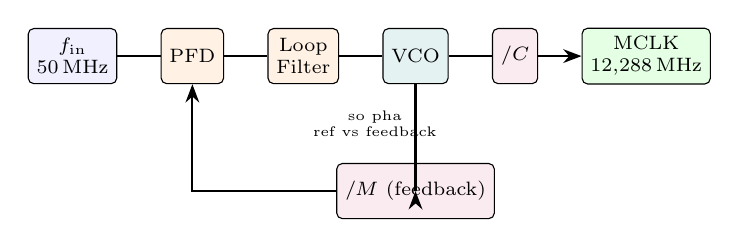
\begin{tikzpicture}[font=\scriptsize,>=Stealth,node distance=0.7cm and 0.55cm]
  \tikzset{box/.style={draw,rounded corners=2pt,align=center,inner sep=3pt,minimum height=0.7cm}}
  \node[box,fill=blue!6] (xin) {$f_{\mathrm{in}}$\\$50\,\text{MHz}$};
  \node[box,fill=orange!10,right=of xin] (pfd) {PFD};
  \node[box,fill=orange!10,right=of pfd] (lf) {Loop\\Filter};
  \node[box,fill=teal!10,right=of lf] (vco) {VCO};
  \node[box,fill=purple!8,right=of vco] (cdiv) {$/C$};
  \node[box,fill=green!10,right=of cdiv] (out) {MCLK\\$12{,}288\,\text{MHz}$};
  \node[box,fill=purple!8,below=1.0cm of vco] (mdiv) {$/M$ (feedback)};
  \draw[->,thick] (xin)--(pfd)--(lf)--(vco)--(cdiv)--(out);
  \draw[->,thick] (vco)|-(mdiv);
  \draw[->,thick] (mdiv)-|(pfd);
  \node[font=\tiny,align=center] at ($(pfd)!0.5!(mdiv)+(0.9,0)$) {so pha\\ref vs feedback};
\end{tikzpicture}
\caption{Luồng tín hiệu trong PLL: PFD so sánh cạnh tham chiếu với feedback sau chia $M$; khi khóa, chia $C$ cho ra MCLK dùng cho codec.}
\label{fig:ch02_pll_loop}
\end{figure}

\paragraph{Ví dụ tính tay --- trôi mẫu theo ppm.} Giả sử sai số MCLK là $\varepsilon=50\,\text{ppm}=50\cdot10^{-6}$. Trong $T=60\,\text{s}$ ở tần số lấy mẫu xử lý $f_s=16\,\text{kHz}$, số mẫu bị trôi tuyệt đối là
\[
\Delta N = \varepsilon\cdot T\cdot f_s = 50\cdot10^{-6}\cdot 60\cdot 16000 = 48\text{ mẫu}.
\]
Bốn mươi tám mẫu ở $16\,\text{kHz}$ tương đương $3\,\text{ms}$ --- đủ để lệch một phần đáng kể của bước nhảy khung $H=160$ mẫu ($10\,\text{ms}$). Với sai số integer-N ở trên ($\approx 0{,}212\,\text{ppm}$):
\[
\Delta N \approx 0{,}212\cdot10^{-6}\cdot 60\cdot 16000 \approx 0{,}204\text{ mẫu/phút},
\]
không đáng kể so với $48$. Mục tiêu lab: giữ sai số audio dưới $5\,\text{ppm}$ ($\Delta N\approx 4{,}8$ mẫu/phút), và luôn chờ tín hiệu \texttt{locked} của PLL trước khi bật FSM I\textsuperscript{2}S. Nếu bỏ qua \texttt{locked}, vài trăm miligiây đầu sau reset MCLK chưa ổn định --- codec ghi rác vào FIFO và đỉnh tự tương quan nhảy lung tung.

\paragraph{IP Altera PLL --- tham số thật.} Trong IP Catalog chọn PLL Intel FPGA IP (hoặc ALTPLL trên tool cũ): Reference Clock $50\,\text{MHz}$; Output $c0=12{,}288\,\text{MHz}$ (đưa chân MCLK codec); có thể thêm $c1=50\,\text{MHz}$ hệ thống nếu muốn cùng nguồn khóa pha với audio (giảm drift tương đối giữa datapath và MCLK). Bật cổng \texttt{locked}; nối \texttt{areset} về nút reset toàn cục đã đồng bộ. Báo cáo PLL List ghi rõ $M,N,C$, $f_{\mathrm{VCO}}$, ppm residual --- lab phải chép các số này vào sổ, không đoán.

\paragraph{RTL và twin.} RTL chỉ được \emph{chia} sau khi đã có MCLK (ví dụ tạo SCLK $= \mathrm{MCLK}/4$ cho frame 64~bit), không thay VCO bằng counter. Mô hình twin Python không mô phỏng jitter analog; nó giả lập trôi thời gian lấy mẫu
\[
t_n = \frac{n}{f_s}\bigl(1+\varepsilon_{\mathrm{ppm}}\cdot 10^{-6}\bigr)
\]
rồi nội suy sóng hình sin $F_0$ biết trước lên lưới $t_n$ lệch và quan sát độ lệch cao độ ước lượng khi $\varepsilon\neq 0$. Script \texttt{verify/verify\_chuong\_02.py} kiểm mọi số ppm/drift nêu trong chương.

\begin{costbox}
\textbf{Ngân sách --- PLL.} Một Fractional PLL cứng trên chip (Cyclone~V 5CSXFC6D6F31C6N có 6 PLL; luồng $F_0$ dùng 1, chiếm $16{,}7\%$ ngân sách PLL theo bảng Chương~0). Logic quanh \texttt{locked} và reset: vài ALM. 0 DSP, 0 M10K. Vì sao bắt buộc IP: soft-counter không đạt độ ổn định ppm và jitter của VCO silicon cho MCLK audio; tự viết PLL bằng RTL là lỗi thiết kế, không phải ``bài tập nâng cao''.
\end{costbox}

\subsection*{2.2. Giao thức I\textsuperscript{2}S với codec WM8731}

\begin{physicalinsight}
Sau khi ADC trong WM8731 đã lượng tử hóa sóng âm, dữ liệu không nhảy sang FPGA dưới dạng mảng số nguyên song song, mà đi trên ba dây nối tiếp theo chuẩn \textbf{I\textsuperscript{2}S} (\emph{Inter-IC Sound} --- đã giới thiệu ở Chương~0): dây \textbf{SCLK}/BCLK chốt từng bit, dây \textbf{WS}/LRCK chọn kênh trái/phải, dây \textbf{SDAT} mang dòng bit. Đây là quy ước giao diện điện tử, không phải hiện tượng dây thanh; nhưng đếm sai một bit hoặc trễ sai một cạnh SCLK sẽ làm hỏng mẫu Q1.15 trước khi tín hiệu kịp vào DC-blocker. Cấu hình thanh ghi codec (định dạng I\textsuperscript{2}S, độ dài word, master/slave clock) đi qua bus \textbf{I\textsuperscript{2}C} riêng --- lab phải khởi tạo I\textsuperscript{2}C trước khi kỳ vọng SDAT có nghĩa.
\end{physicalinsight}

\paragraph{Quan hệ đồng hồ.} Với cấu hình stereo phổ biến trên DE10 (mỗi slot 32~bit, hai kênh = 64 bit/frame) tại $f_s=48\,\text{kHz}$:
\begin{align*}
\mathrm{MCLK} &= 256\cdot f_s = 256\cdot 48000 = 12{,}288{,}000\,\text{Hz},\\
\mathrm{SCLK} &= 64\cdot f_s = 64\cdot 48000 = 3{,}072{,}000\,\text{Hz}.
\end{align*}
Nếu lab chỉ lấy 16~bit/kênh (32 bit/frame tổng cộng L+R) thì $\mathrm{SCLK}=32\cdot f_s=1{,}536{,}000\,\text{Hz}$. Chuẩn Philips I\textsuperscript{2}S: MSB đi trước, dữ liệu hợp lệ bắt đầu sau đúng một cạnh SCLK kể từ cạnh đổi của WS. Trên đường ước lượng $F_0$ mono, FSM chỉ chốt kênh Left rồi bỏ Right --- đủ thông tin cao độ, tiết kiệm băng thông FIFO.

\begin{figure}[H]
\centering
\begin{tikzpicture}[font=\scriptsize, x=0.55cm, y=0.55cm]
  \draw[->] (0,4) -- (18,4) node[right] {SCLK};
  \foreach \x in {0,...,16} {\draw (\x,3.85) -- (\x,4.15);}
  \draw[thick,teal!70!black] (0,2.5) -- (1,2.5) -- (1,1.2) -- (9,1.2) -- (9,2.5) -- (17,2.5);
  \node[left,teal!70!black] at (0,1.85) {WS/LRCK};
  \node[font=\tiny] at (5,0.55) {khung Left};
  \node[font=\tiny] at (13,0.55) {khung Right};
  \foreach \x/\b in {2/1,3/0,4/1,5/1,6/0,7/0,8/1} {
    \draw[blue!70!black,thick] (\x,3.2) -- (\x,3.6);
    \node[blue!70!black,font=\tiny] at (\x,3.0) {\b};
  }
  \node[blue!70!black,font=\tiny,align=center] at (5,4.7) {bit MSB$\ldots$ (trễ 1 SCLK sau cạnh WS)};
  \draw[->,orange!80!black,thick] (1,2.5) -- ++(0,0.9) -- ++(1,0);
  \node[orange!80!black,font=\tiny] at (2.8,3.55) {+1 SCLK};
\end{tikzpicture}
\caption{Timing I\textsuperscript{2}S đơn giản hóa: cạnh WS mở khung Left; dữ liệu trên SDAT hợp lệ bắt đầu sau đúng một cạnh SCLK (chuẩn Philips).}
\label{fig:ch02_i2s_timing}
\end{figure}

\paragraph{Ví dụ tính tay --- đóng gói nibble rồi word Q1.15.} Bốn cạnh SCLK liên tiếp nhận các bit $1,0,1,1$ (MSB trước). Thanh ghi dịch trái lần lượt:
\[
0 \to 1 \to 2 \to 5 \to 11 \quad (0\mathrm{b}1011 = 11_{10}).
\]
Mười sáu bit MSB của slot Left mang mẫu có dấu. Ví dụ bit-stream $0100\,0000\,0000\,0000$ (MSB trước) đóng thành
\[
0\mathrm{b}0100\,0000\,0000\,0000 = 16384_{10},
\]
đúng mức $0{,}5$ trong Q1.15 (ô Feynman~7, Chương~0). Lab lấy 16 bit cao của slot 32~bit (bỏ 16 bit đệm thấp) rồi đẩy vào DCFIFO.

\paragraph{Hai lộ trình phần cứng.} (1)~\textbf{University Program Audio Core}: IP Avalon bọc cấu hình I\textsuperscript{2}C của codec và FIFO L/R --- gắn nhanh Platform Designer nhưng che mất đường mẫu, khó đối chiếu bit-exact. (2)~\textbf{RTL tự viết (default dạy)}: FSM Idle$\to$WaitWS$\to$Skip1$\to$Shift16$\to$Push, đồng bộ cạnh WS sang miền SCLK bằng hai flip-flop, dịch 16~bit hữu ích, nâng \texttt{wrreq} mỗi mẫu Left. Twin phần mềm: tệp \texttt{.wav} int16 little-endian chính là đầu ra bit-exact sau khi bỏ padding slot.

\paragraph{RTL giải thích từng nhóm lệnh.}
\begin{verbatim}
// Đồng bộ WS (async từ codec) sang miền SCLK bằng 2FF
reg ws_ff1, ws_ff2, ws_prev;
always @(posedge sclk) begin
  ws_ff1 <= ws_async;   // FF1: hấp thụ metastability
  ws_ff2 <= ws_ff1;     // FF2: bit đã ổn định
  ws_prev <= ws_ff2;    // nhớ cạnh trước để phát hiện rising
end
wire ws_rise = ws_ff2 & ~ws_prev;  // cạnh lên = bắt đầu Left (tùy polarity)

// FSM rút gọn: sau ws_rise chờ 1 SCLK (Philips), rồi dịch 16 bit
// reg [4:0] bit_cnt; reg [15:0] shreg;
// khi bit_cnt==15: data_left <= {shreg[14:0], sdat}; wrreq_fifo <= 1;
\end{verbatim}
Dòng \texttt{ws\_ff1 <= ws\_async} là chỗ metastability được phép xảy ra --- chỉ trên \emph{một} bit điều khiển. Dòng \texttt{ws\_ff2} cho bit thời gian ổn định trước khi dùng. \texttt{ws\_rise} phát hiện cạnh; sau đúng một SCLK (trễ Philips) mới lấy MSB. Khi đủ 16~bit, ghi DCFIFO phía \texttt{wrclk = sclk}. Phía \texttt{rdclk = 50\,MHz} đọc ra Avalon-ST (\texttt{valid}/\texttt{ready}) sang DC-blocker.

\begin{costbox}
\textbf{Ngân sách --- I\textsuperscript{2}S RX.} Vài chục đến khoảng $100$ ALM (shift register 16--32 bit + phát hiện cạnh WS + FSM), 0 DSP, 0 M10K cho khối RX thuần. Chọn mono Left vì ước lượng $F_0$ không cần stereo; stereo sẽ nhân đôi băng thông CDC và số từ FIFO mà không tăng độ chính xác đỉnh tự tương quan. Fmax miền SCLK $3{,}072\,\text{MHz}$ rất dư với silicon tốc độ 6.
\end{costbox}

\subsection*{2.3. CDC: DCFIFO bất đồng bộ và mã Gray}

\begin{physicalinsight}
Miền đồng hồ âm thanh (MCLK $12{,}288\,\text{MHz}$, SCLK $3{,}072\,\text{MHz}$) và miền xử lý lõi ($50\,\text{MHz}$) dao động từ các nguồn độc lập --- chúng \textbf{bất đồng bộ}. Nếu nối một thanh ghi 16~bit từ miền SCLK sang miền $50\,\text{MHz}$ bằng dây thô, một số bit có thể chốt ở trạng thái trung gian khi hai miền ``đụng cạnh'', tạo \textbf{metastability}: giá trị đọc ra không phải 0 cũng không phải 1 ổn định trong thời gian hữu hạn. Hậu quả trên đường $F_0$ là mẫu rác đột biến, đỉnh tự tương quan nhảy lung tung, đôi khi FSM tưởng FIFO full/empty sai.
\end{physicalinsight}

Giải pháp chuẩn là bộ đệm \textbf{DCFIFO} (\emph{Dual-Clock FIFO} --- đã nêu ở Chương~0): cổng ghi chạy theo clock nguồn (SCLK), cổng đọc chạy theo clock đích ($50\,\text{MHz}$). Dữ liệu mẫu nằm trong RAM dual-port nội bộ; cái bắt chéo miền clock \emph{không} phải là word dữ liệu 16~bit mà là \textbf{con trỏ} ghi/đọc. Con trỏ khi bắt chéo miền phải được mã hóa \textbf{mã Gray}: mỗi lần tăng địa chỉ chỉ đúng một bit thay đổi. Nhờ đó, dù bên kia lấy mẫu lúc con trỏ đang chuyển, nó chỉ có thể đọc nhầm tối đa một bước địa chỉ liền kề --- không bao giờ đọc phải từ bit-pattern trung gian vô nghĩa của mã nhị phân thường.

\paragraph{Toán mã Gray.} Với số nguyên không dấu $n$, mã Gray phản xạ là
\[
G(n)=n\oplus\bigl\lfloor n/2\bigr\rfloor = n\oplus(n\gg 1).
\]
Bảng tính tay $n=0\ldots7$ (3 bit):

\begin{center}\small
\begin{tabular}{@{}ccl@{}}
\toprule
$n$ (thập phân) & Nhị phân & Gray $G(n)$ \\
\midrule
0 & 000 & 000 \\
1 & 001 & 001 \\
2 & 010 & 011 \\
3 & 011 & 010 \\
4 & 100 & 110 \\
5 & 101 & 111 \\
6 & 110 & 101 \\
7 & 111 & 100 \\
\bottomrule
\end{tabular}
\end{center}

Hai mã Gray liên tiếp luôn khác đúng một bit: ví dụ $G(3)=010$ và $G(4)=110$ chỉ khác bit cao. Đảo ngược Gray$\to$binary trên giấy: $b_2=g_2$, $b_1=g_2\oplus g_1$, $b_0=g_2\oplus g_1\oplus g_0$.

\paragraph{Nội tại DCFIFO Intel --- đồng bộ con trỏ.} IP FIFO (dcfifo) thực hiện đúng chuỗi sau mỗi lần ghi/đọc:
\begin{enumerate}[leftmargin=1.4em]
  \item Tăng con trỏ nhị phân phía local clock ($wrptr$ hoặc $rdptr$).
  \item Đổi sang Gray: $wrptr\_gray = G(wrptr)$.
  \item Đưa $wrptr\_gray$ qua chuỗi \textbf{hai flip-flop} sang miền clock bên kia (đúng chuẩn 2FF CDC cho từng bit Gray --- vì mỗi bit Gray chỉ đổi đơn lẻ, metastability trên một bit không kéo theo bit khác).
  \item Ở miền đích, đổi Gray$\to$binary rồi so với con trỏ local để tính \texttt{wrfull}/\texttt{rdempty}/\texttt{rdusedw}.
\end{enumerate}
Word dữ liệu 16~bit \emph{không} đi qua 2FF: nó nằm trong dual-port RAM, được ghi theo địa chỉ binary phía write và đọc theo địa chỉ binary phía read; chỉ có ``vé địa chỉ'' (con trỏ Gray) là tín hiệu bất đồng bộ cần đồng bộ hóa.

\begin{figure}[H]
\centering
\begin{tikzpicture}[font=\scriptsize,>=Stealth, node distance=0.55cm and 0.7cm]
  \tikzset{box/.style={draw,rounded corners=2pt,align=center,inner sep=3pt}}
  \node[box,fill=blue!8] (wclk) {wrclk\\(SCLK)};
  \node[box,fill=orange!12,right=of wclk] (wbin) {wrptr\\binary};
  \node[box,fill=yellow!20,right=of wbin] (wgray) {$G(wrptr)$};
  \node[box,fill=red!12,right=of wgray] (ff1) {2FF\\CDC};
  \node[box,fill=yellow!20,right=of ff1] (wsync) {Gray\\synced};
  \node[box,fill=orange!12,right=of wsync] (wdec) {bin\\decode};
  \node[box,fill=green!12,below=1.1cm of wdec] (cmp) {so khớp\\full/empty};
  \node[box,fill=teal!12,left=of cmp] (rbin) {rdptr\\(rdclk)};
  \node[box,fill=purple!10,below=1.1cm of wbin] (ram) {DP-RAM\\data[15:0]};
  \draw[->] (wclk)--(wbin)--(wgray)--(ff1)--(wsync)--(wdec)--(cmp);
  \draw[->] (rbin)--(cmp);
  \draw[->] (wbin)|-(ram);
  \draw[->] (rbin)|-(ram);
  \node[font=\tiny,align=left,anchor=west] at (-0.2,-2.6)
    {Chỉ con trỏ Gray đi qua 2FF; mẫu PCM nằm trong DP-RAM theo địa chỉ binary local.};
\end{tikzpicture}
\caption{Luồng CDC trong DCFIFO: mã hóa Gray $\to$ đồng bộ 2FF từng bit $\to$ giải mã binary $\to$ so full/empty; dữ liệu mẫu không bắt chéo thô.}
\label{fig:ch02_dcfifo_gray}
\end{figure}

\paragraph{Ví dụ tính tay --- vì sao nhị phân thường nguy hiểm.} Con trỏ nhị phân từ $3$ ($011$) lên $4$ ($100$) đổi \emph{cả ba bit} cùng lúc. Bên đọc bắt chéo miền có thể chốt thành $000$, $111$, $001$,\ldots --- địa chỉ giả cách xa hàng đợi thật, đọc nhầm mẫu cũ hoặc đè cờ full/empty. Với Gray, bước $010\to 110$ chỉ một bit; sai lệch tối đa là $\pm 1$ ô.

\paragraph{Ví dụ tính tay --- chọn depth.} Tốc độ ghi mono $=48\,\text{kHz}$. Giả sử jitter tương đối và burst đọc phía hệ thống tạo độ trễ hấp thụ tối đa $100\,\mu\mathrm{s}$. Số mẫu cần đệm:
\[
N_{\mathrm{depth}}\ge 48000\cdot 100\cdot 10^{-6}=4{,}8 \quad\Rightarrow\quad \text{chọn depth }8\text{ hoặc }16.
\]
Depth 8 từ $\times 16$~bit $=128$~bit --- vừa một MLAB; không cần M10K. Lab mặc định depth~16 để dư margin khi FSM phía đọc thỉnh thoảng \texttt{ready}=0.

\paragraph{Twin Python (mô hình logic, không mô phỏng metastability analog).}
\begin{verbatim}
def bin_to_gray(n):
    return n ^ (n >> 1)

# Kiểm bảng 0..7 và tính chất một bit
grays = [bin_to_gray(i) for i in range(8)]
assert [format(g, "03b") for g in grays] == [
    "000","001","011","010","110","111","101","100"]
for a, b in zip(grays, grays[1:]):
    assert bin(a ^ b).count("1") == 1
\end{verbatim}
Twin mức hệ thống: hàng đợi \texttt{collections.deque} với hai ``clock tick'' độc lập; assert không đọc khi empty và không ghi khi full --- tương ứng cờ IP.

\begin{costbox}
\textbf{Ngân sách --- CDC.} FIFO nông (8--16 từ $\times 16$~bit): thường map vào 1 MLAB hoặc một phần M10K tùy depth. Logic Gray + full/empty + 2FF: vài chục ALM. 0 DSP. Vì sao không đủ 2FF cho cả word dữ liệu: 2FF chỉ an toàn cho một bit điều khiển; word 16~bit cần FIFO/Gray để toàn bộ mẫu nhất quán theo đúng thứ tự ghi. Latency CDC: vài chu kỳ clock đích (2FF + logic empty) --- không đáng kể so với $500\,000$ chu kỳ/hop.
\end{costbox}

\subsection*{2.4. Chi phí tổng hợp và chỗ đứng trong đường tín hiệu}

Khối Chương~2 nằm ngay sau codec và trước DC-blocker (xem bản đồ Hình ở Chương~0). Toàn bộ PLL + I\textsuperscript{2}S RX + DCFIFO tiêu tốn khoảng 1 PLL cứng, $<150$ ALM, 0 DSP, và tối đa 1 MLAB/M10K cho FIFO --- cố tình giữ rẻ để dành DSP và M10K cho FIR (Chương~4) và MAC tự tương quan (Chương~7). Fmax phía sysclk dễ vượt $150\,\text{MHz}$; điểm nghẽn thật sự là kỷ luật CDC và việc chờ \texttt{locked}, không phải diện tích. RTF phần thu thập gần bằng $1$ nếu FSM không bỏ mẫu: mỗi mẫu audio vào đúng một mẫu ra phía DC-blocker khi \texttt{ready} luôn sẵn.

\subsection*{2.5. Bài tập và lời giải giải thích}

\paragraph{Bài tập 2.1 (Tỷ số PLL và sai số ppm).}
Từ thạch anh $f_{\mathrm{in}}=50\,\text{MHz}$, kỹ sư cần MCLK $=12{,}288\,\text{MHz}$.
\begin{enumerate}[label=\alph*)]
  \item Tính tỷ số $M/(N\cdot C)$ lý thuyết.
  \item Nếu dùng integer-N với $M=1507$, $N=73$, $C=84$, tần số thực tế là bao nhiêu và sai số so với $12{,}288\,\text{MHz}$ tính bằng ppm?
  \item Trong 60 giây ở $16\,\text{kHz}$, sai số đó làm trôi bao nhiêu mẫu? So với trường hợp $50\,\text{ppm}$ thuần.
\end{enumerate}
\paragraph{Lời giải giải thích.}
\begin{enumerate}[label=\alph*)]
  \item $M/(N\cdot C)=12{,}288/50=0{,}24576$.
  \item $f_{\mathrm{out}}=50\cdot 1507/(73\cdot 84)\approx 12{,}28799739\,\text{MHz}$. Sai số
  $\varepsilon_{\mathrm{ppm}}\approx 0{,}212\,\text{ppm}$ (script \texttt{verify\_chuong\_02.py}).
  \item $\Delta N\approx 0{,}204$ mẫu/phút --- không đáng kể so với $48$ mẫu/phút khi sai $50\,\text{ppm}$. Fractional PLL vẫn tiện hơn vì MegaWizard điền đúng $12{,}288$.
\end{enumerate}

\paragraph{Bài tập 2.2 (SCLK và nibble I\textsuperscript{2}S).}
Codec chạy $f_s=48\,\text{kHz}$, frame stereo 64 bit.
\begin{enumerate}[label=\alph*)]
  \item Tính SCLK.
  \item Dịch bốn bit $1,0,1,1$ (MSB trước) --- giá trị thập phân?
  \item Bit-stream 16 bit $0100\,0000\,0000\,0000$ đóng thành số Q1.15 nào?
  \item Vì sao lab mono Left đủ cho $F_0$?
\end{enumerate}
\paragraph{Lời giải giải thích.}
\begin{enumerate}[label=\alph*)]
  \item $\mathrm{SCLK}=64\cdot 48000=3{,}072{,}000\,\text{Hz}$.
  \item $0\mathrm{b}1011=11_{10}$.
  \item $16384$ --- đúng mức $0{,}5$ trong Q1.15.
  \item Cao độ là thuộc tính nguồn kích thích dây thanh, gần như đồng nhất trên hai kênh micro gần nhau; lấy thêm Right chỉ nhân đôi băng thông CDC.
\end{enumerate}

\paragraph{Bài tập 2.3 (Gray và metastability).}
Con trỏ FIFO 3~bit tăng từ $3$ lên $4$.
\begin{enumerate}[label=\alph*)]
  \item Viết mã nhị phân và mã Gray của hai giá trị.
  \item Giải thích tại sao bắt chéo miền clock trên mã nhị phân có thể đọc ra địa chỉ xa, còn Gray thì không.
\end{enumerate}
\paragraph{Lời giải giải thích.}
\begin{enumerate}[label=\alph*)]
  \item Nhị phân: $3=011$, $4=100$ (đổi 3 bit). Gray: $G(3)=010$, $G(4)=110$ (đổi 1 bit).
  \item Nhiều bit đổi cùng lúc cho phép tổ hợp trung gian bất kỳ (địa chỉ xa). Gray bảo đảm mọi thời điểm trung gian chỉ sai tối đa một bước liền kề --- lý do DCFIFO Intel gray-code hóa con trỏ xuyên miền.
\end{enumerate}

\paragraph{Bài tập 2.4 (Depth FIFO và 2FF).}
\begin{enumerate}[label=\alph*)]
  \item Với mono $48\,\text{kHz}$ và jitter hấp thụ $100\,\mu\mathrm{s}$, depth tối thiểu lý thuyết là bao nhiêu? Lab chọn 8 hay 16 thì vì sao?
  \item Vì sao chuỗi 2FF áp dụng cho từng bit Gray chứ không cho cả word mẫu 16~bit?
\end{enumerate}
\paragraph{Lời giải giải thích.}
\begin{enumerate}[label=\alph*)]
  \item $48000\cdot 100\cdot 10^{-6}=4{,}8$ --- tối thiểu 5, chọn 8 hoặc 16 để dư margin khi \texttt{ready}=0 phía đọc. Depth 16 an toàn hơn khi FSM FIR/DC thỉnh thoảng dừng.
  \item 2FF chỉ đảm bảo một bit điều khiển thoát metastability; 16 bit dữ liệu có thể mỗi bit ổn định ở giá trị khác nhau tạo word rác. FIFO giữ data trong RAM và chỉ đồng bộ con trỏ Gray.
\end{enumerate}

\paragraph{Bài tập 2.5 (\texttt{locked} và trôi $5\,\text{ppm}$).}
\begin{enumerate}[label=\alph*)]
  \item Tính $\Delta N$ trong 60~s ở $16\,\text{kHz}$ nếu sai số còn $5\,\text{ppm}$.
  \item FSM I\textsuperscript{2}S có được phép chạy khi \texttt{locked}=0 không? Giải thích hậu quả.
\end{enumerate}
\paragraph{Lời giải giải thích.}
\begin{enumerate}[label=\alph*)]
  \item $\Delta N=5\cdot10^{-6}\cdot 60\cdot 16000=4{,}8$ mẫu/phút --- mục tiêu lab chấp nhận được.
  \item Không. Khi chưa \texttt{locked}, MCLK lệch mạnh hoặc dừng; codec xuất bit vô nghĩa, FIFO đầy mẫu rác, đỉnh $\mathcal{R}[\tau]$ không ổn định. Phải AND \texttt{locked} vào tín hiệu enable của FSM thu.
\end{enumerate}

\clearpage
\phantomsection
\section*{Chương 3. DC-blocker IIR (cực/zero, accumulator 32-bit)}
\addcontentsline{toc}{section}{Chương 3. DC-blocker IIR (cực/zero, accumulator 32-bit)}
\pdfbookmark[1]{Chương 3. DC-blocker IIR (cực/zero, accumulator 32-bit)}{chuong3}

\begin{learningobj}
Sau Chương~3, người học giải thích được vì sao offset một chiều phá đỉnh tự tương quan, viết đúng hàm truyền một cực--một zero với $\alpha=1-2^{-8}$, hiện thực RTL accumulator 32~bit theo công thức $y_{\mathrm{acc}}\leftarrow y_{\mathrm{acc}}+x_{\Delta}-(y_{\mathrm{acc}}\ggg 8)$ rồi $\mathrm{sat}_{16}(y_{\mathrm{acc}}\ggg 15)$, và đối chiếu bit-exact với twin Python. Khái niệm điểm cực/điểm không và Avalon-ST đã có ở ô Feynman~12 của Chương~0.
\end{learningobj}

\subsection*{3.1. Hiện tượng: offset DC nuốt đỉnh chu kỳ}

\begin{physicalinsight}
Micro, codec WM8731 và đường dây analog luôn cộng thêm một thành phần gần đứng yên: điện áp offset một chiều (DC), cộng thêm trôi chậm do nhiệt. Trong miền mẫu, đó là một hằng $A$ cộng vào mọi $x[n]$. Phép tự tương quan (ô Feynman~5, Chương~0) không phân biệt năng lượng hữu ích và năng lượng offset. Nếu $A$ lớn, đỉnh tại độ trễ $\tau=0$ phình theo $A^2$ và có thể át hoàn toàn đỉnh chu kỳ $T_0$ của dây thanh --- thuật toán sẽ báo vô thanh hoặc treo ở cao độ sai.
\end{physicalinsight}

Viết tường minh với tín hiệu $x[n]+A$:
\begin{align*}
\mathcal{R}_{x+A}[0]
&=\sum_{n=0}^{N-1}(x[n]+A)^2\\
&=\sum_{n=0}^{N-1}x[n]^2 + 2A\sum_{n=0}^{N-1}x[n] + N A^2
=\mathcal{R}_x[0]+2A\sum_n x[n]+N A^2.
\end{align*}
Số hạng $N A^2$ luôn dương và tỉ lệ với bình phương offset. Praat trừ mean cục bộ từng khung; trên FPGA streaming ta dùng bộ lọc IIR liên tục gọi là \textbf{DC-blocker}: một bộ thông cao rất nhẹ, ổn định, rẻ silicon, đặt ngay sau I\textsuperscript{2}S/CDC.

\begin{figure}[H]
\centering
\begin{tikzpicture}[font=\small]
  \begin{scope}
    \draw[->] (0,0) -- (5.2,0) node[right] {$\tau$};
    \draw[->] (0,0) -- (0,2.8) node[above] {$\mathcal{R}$};
    \draw[thick, red!70!black] (0,2.4) -- (0.15,2.4) -- (0.3,0.4) -- (1,0.35) -- (2,0.9) -- (3,0.3) -- (4,0.25);
    \node[font=\footnotesize\bfseries] at (2.5,3.15) {Trước DC-block: $\mathcal{R}[0]$ phình};
  \end{scope}
  \begin{scope}[xshift=7.2cm]
    \draw[->] (0,0) -- (5.2,0) node[right] {$\tau$};
    \draw[->] (0,0) -- (0,2.8) node[above] {$\mathcal{R}$};
    \draw[thick, teal!70!black] (0,1.2) -- (0.2,0.3) -- (1,0.25) -- (2,1.8) -- (3,0.3) -- (4,0.25);
    \node[font=\footnotesize\bfseries] at (2.5,3.15) {Sau: đỉnh $T_0$ lộ rõ};
    \node[teal!60!black, font=\scriptsize] at (2,2.15) {$T_0$};
  \end{scope}
\end{tikzpicture}
\caption{Cùng một tín hiệu có offset: bên trái đỉnh $\tau=0$ nuốt chu kỳ; bên phải sau DC-blocker đỉnh $T_0$ hiện ra để Chương~9 nội suy.}
\label{fig:ch03_dc_before_after}
\end{figure}

\paragraph{Ví dụ tính tay --- DC thuần phá $\mathcal{R}[0]$.} Chuỗi $x=[1,1,1,1]$ (toàn DC) cho $\mathcal{R}[0]=\sum x_n^2=4$. Sau khi trừ mean (mọi mẫu về 0) thì $\mathcal{R}[0]=0$: DC thuần phải đi tiếp như tín hiệu vô thanh, không được nuôi FSM cao độ bằng năng lượng giả.

\subsection*{3.2. Toán: cực, zero và chọn $\alpha=1-2^{-8}$}

Hàm truyền chuẩn của DC-blocker bậc nhất:
\[
H(z)=\frac{1-z^{-1}}{1-\alpha z^{-1}},\qquad 0<\alpha<1.
\]
\textbf{Zero} (nghiệm tử số) tại $z=1$ --- đúng tần số $0\,\text{Hz}$ --- nên $H(1)=0$: mọi tín hiệu hoàn toàn đứng yên bị triệt tiêu. \textbf{Cực} (nghiệm mẫu số) tại $z=\alpha$, nằm sát zero nhưng vẫn trong vòng đơn vị nên bộ lọc ổn định. Phương trình sai phân tương đương:
\[
y[n]=x[n]-x[n-1]+\alpha\, y[n-1].
\]

\begin{figure}[H]
\centering
\begin{tikzpicture}[scale=1.35]
  \draw[thick] (0,0) circle (1.5);
  \draw[->] (-2.0,0) -- (2.2,0) node[right] {$\mathrm{Re}$};
  \draw[->] (0,-1.9) -- (0,1.9) node[above] {$\mathrm{Im}$};
  \node[below left] at (0,0) {$0$};
  \draw[very thick, blue!70!black] (1.5,0.12) -- (1.5,-0.12);
  \draw[very thick, blue!70!black] (1.38,0) -- (1.62,0);
  \node[above right,blue!70!black] at (1.5,0.15) {zero $z=1$};
  \filldraw[red!70!black] (1.494,0) circle (0.055);
  \node[below,red!70!black,font=\small] at (1.35,-0.18) {cực $z=\alpha=1-2^{-8}$};
  \node[align=left, font=\small] at (-0.15,-2.35)
    {Zero trên vòng đơn vị tại DC $\Rightarrow H(1)=0$.\\
     Cực gần zero (trong vòng) $\Rightarrow$ HPF nhẹ, ổn định.};
\end{tikzpicture}
\caption{DC-blocker trên mặt phẳng $z$: zero tại $z=1$, cực tại $\alpha=1-2^{-8}=0{,}99609375$.}
\label{fig:ch03_zplane}
\end{figure}

Trên silicon ta chọn $\alpha=1-2^{-8}=0{,}99609375$ vì phép nhân $\alpha\cdot y$ thu gọn thành một phép dịch và trừ:
\[
\alpha y = y - (y\ggg 8) = y\cdot(1-2^{-8}),
\]
không tốn khối DSP. Hằng thời gian xấp xỉ $1/(1-\alpha)=256$ mẫu. Tại $f_s=16\,\text{kHz}$ (sau FIR), cutoff xấp xỉ
\[
f_c\approx\frac{1-\alpha}{2\pi}f_s=\frac{2^{-8}}{2\pi}\cdot 16000\approx 9{,}95\,\text{Hz},
\]
nằm dưới $F_{0,\min}=75\,\text{Hz}$ và trên DC --- đúng chỗ cần chặn. (Ở $48\,\text{kHz}$ ngay sau codec, $f_c\approx 29{,}8\,\text{Hz}$, vẫn an toàn trước khi hạ mẫu.)

\paragraph{Ví dụ tính tay --- đáp ứng xung với $\alpha=0{,}5$ (cực xa để thấy nhanh).} Cho $x=\delta[n]$ hiệu dụng qua công thức $y[n]=(x[n]-x[n-1])+\alpha y[n-1]$ với đầu vào hằng $x=[1,1,1,1,1]$, $y[-1]=0$:
\begin{center}\small
\begin{tabular}{@{}rlll@{}}
\toprule
$n$ & $x[n]$ & $y[n]=(x[n]-x[n-1])+\alpha y[n-1]$ & giá trị \\
\midrule
0 & 1 & $1-0+0$ & $1$ \\
1 & 1 & $0+0{,}5\cdot 1$ & $0{,}5$ \\
2 & 1 & $0+0{,}5\cdot 0{,}5$ & $0{,}25$ \\
3 & 1 & $0+0{,}5\cdot 0{,}25$ & $0{,}125$ \\
4 & 1 & $0+0{,}5\cdot 0{,}125$ & $0{,}0625$ \\
\bottomrule
\end{tabular}
\end{center}
Năng lượng bị nuốt theo cấp số nhân về 0 --- đúng trực giác HPF nhớ trạng thái. Với $\alpha=0{,}99609375$ suy giảm chậm hơn khoảng $256$ lần mẫu.

\subsection*{3.3. Phần cứng: vì sao accumulator 32-bit và RTL}

FIR Compiler II không thay thế được IIR có phản hồi: kiến trúc FIR không có vòng $y[n-1]$. Viết khoảng mười dòng Verilog với accumulator 32~bit là lựa chọn dạy và lab.

Nếu giữ $y$ chỉ 16~bit Q1.15, mỗi lần nhân $\alpha$ (hay dịch $\ggg 8$) sẽ cắt mất phần thập phân khi $|y|$ nhỏ, tạo vùng chết (deadband) hoặc dao động limit-cycle. Giải pháp: giữ thanh ghi phản hồi \texttt{y\_acc} signed 32~bit; mẫu vào Q1.15 được kéo lên cùng thang bằng dịch trái 15~bit trước khi trừ; ngõ ra lấy lại Q1.15 bằng dịch phải 15~bit rồi bão hòa.

\paragraph{Phương trình bit-exact (khớp assignment và twin).}
\begin{align*}
x_{\Delta} &= (x[n]\ll 15)-(x[n-1]\ll 15),\\
y_{\mathrm{acc}}[n] &= y_{\mathrm{acc}}[n-1] + x_{\Delta} - (y_{\mathrm{acc}}[n-1]\ggg 8),\\
y_{\mathrm{out}} &= \mathrm{sat}_{16}(y_{\mathrm{acc}}[n]\ggg 15),
\end{align*}
với $\mathrm{sat}_{16}$ ghim vào $[-32768,+32767]$. Trên số có dấu, toán tử Python/NumPy \texttt{>>} và Verilog \texttt{>>>} cùng là arithmetic floor shift.

\begin{verbatim}
module dc_blocker (
  input  wire               clk, rst_n,
  input  wire               in_valid,
  output wire               in_ready,
  input  wire signed [15:0] x_in,       // Q1.15
  output reg                out_valid,
  input  wire               out_ready,
  output reg  signed [15:0] y_out
);
  reg signed [15:0] x_z1;
  reg signed [31:0] y_acc;              // 32-bit feedback (NOT 16)
  assign in_ready = out_ready | ~out_valid;

  wire signed [31:0] x_delta =
      ($signed({x_in, 15'b0})) - ($signed({x_z1, 15'b0}));
  wire signed [31:0] y_next =
      y_acc + x_delta - (y_acc >>> 8);
  wire signed [31:0] y_shift = y_next >>> 15;

  function automatic signed [15:0] sat16;
    input signed [31:0] v;
    begin
      if (v > 32'sd32767)       sat16 = 16'sd32767;
      else if (v < -32'sd32768) sat16 = -16'sd32768;
      else                      sat16 = v[15:0];
    end
  endfunction

  always @(posedge clk or negedge rst_n) begin
    if (!rst_n) begin
      x_z1 <= 0; y_acc <= 0; y_out <= 0; out_valid <= 0;
    end else if (in_valid && in_ready) begin
      y_acc <= y_next;
      x_z1  <= x_in;
      y_out <= sat16(y_shift);
      out_valid <= 1'b1;
    end else if (out_valid && out_ready) out_valid <= 1'b0;
  end
endmodule
\end{verbatim}

\subsection*{3.4. Twin Python bit-exact và ví dụ step Q1.15}

\begin{verbatim}
import numpy as np

def sat16(v):
    return int(np.clip(v, -32768, 32767))

def dc_blocker_q15(x, alpha_shift=8):
    """x: int16 Q1.15. y_acc int32.
    y_acc += x_delta - (y_acc >> 8); out = sat16(y_acc >> 15)
    với x_delta = (x<<15) - (x_z1<<15)."""
    y_acc = np.int32(0)
    x_z1 = np.int32(0)
    out = np.empty(len(x), dtype=np.int16)
    for i, xi in enumerate(np.asarray(x, dtype=np.int32)):
        dx = np.int32((xi << 15) - (x_z1 << 15))
        y_acc = np.int32(y_acc + dx - (y_acc >> alpha_shift))
        x_z1 = xi
        out[i] = sat16(int(y_acc >> 15))
    return out
\end{verbatim}

\paragraph{Ví dụ tính tay khớp bit.} Đầu vào $[0,0,0]$ rồi bước DC $16384$ ($0{,}5$ trong Q1.15). Ba mẫu đầu ra $0$. Tại mẫu bước ($n=3$): $x_{\Delta}=16384\ll 15=536870912$, $y_{\mathrm{acc}}=536870912$, $y_{\mathrm{out}}=16384$. Mẫu kế:
\[
y_{\mathrm{acc}}\leftarrow 536870912 + 0 - (536870912\ggg 8)=534773760,\quad
y_{\mathrm{out}}=534773760\ggg 15=16320.
\]
Mẫu tiếp: $y_{\mathrm{out}}=16256$. Dãy $16384,16320,16256,\ldots$ giảm khoảng $64$ mỗi bước lúc đầu --- đúng $\alpha=1-2^{-8}$. Sau khoảng $5\cdot 256$ mẫu, đầu ra tụt dưới $50$ LSB (script \texttt{verify/verify\_chuong\_03.py}).

\begin{costbox}
\textbf{Ngân sách --- DC-blocker.} Adder/sub 32~bit + dịch số học: khoảng $80$--$120$ ALM (thường vài chục đến $\sim 100$). 0 DSP (nhờ $\alpha=1-2^{-8}$). 0 M10K. Latency: 1 mẫu (pipeline Avalon-ST một nhịp). Fmax dễ $>200\,\text{MHz}$. Vì sao không cắt 16~bit sớm: tiết kiệm $\sim 30$ ALM nhưng sai chức năng (deadband) --- đắt hơn mọi LUT trên đường $F_0$.
\end{costbox}

\subsection*{3.5. Bài tập và lời giải giải thích}

\paragraph{Bài tập 3.1 (Phình $\mathcal{R}[0]$.)}
Cho $x_0=[1,-1,1,-1]$ và offset $A=2$. Tính $\sum(x_0[n]+A)^2$ và giải thích vì sao DC-blocker phải đứng trước MAC.
\paragraph{Lời giải.} $\sum(x_0+A)^2=(3)^2+(1)^2+(3)^2+(1)^2=9+1+9+1=20$, trong khi $\sum x_0^2=4$. Offset đã nhân năng lượng $\tau=0$ lên năm lần; không chặn DC thì ngưỡng voicing và đỉnh $T_0$ đều lệch.

\paragraph{Bài tập 3.2 (Đệ quy $\alpha=0{,}5$).}
Với $x=[1,1,1,1,1]$, $\alpha=0{,}5$, $y[-1]=0$, lập bảng $y[0..4]$. Nhận xét giới hạn khi $n\to\infty$.
\paragraph{Lời giải.} $1,\ 0{,}5,\ 0{,}25,\ 0{,}125,\ 0{,}0625$ --- cấp số nhân công bội $1/2$, tiến về $0$: DC thuần bị nuốt hết.

\paragraph{Bài tập 3.3 (Bit-exact step).}
Dùng công thức $y_{\mathrm{acc}}\mathrel{+}=x_{\Delta}-(y_{\mathrm{acc}}\ggg 8)$, $x_{\Delta}=(x\ll 15)-(x_{z1}\ll 15)$, tính $y_{\mathrm{out}}$ tại hai mẫu đầu của bước $16384$ (sau ba số 0).
\paragraph{Lời giải.} $y_{\mathrm{out}}[3]=16384$, $y_{\mathrm{out}}[4]=16320$ (đã kiểm script). Sai số một LSB ở đây đồng nghĩa twin và RTL lệch thang cố định điểm --- bắt buộc khớp trước khi nối FIR.

\clearpage
\phantomsection
\section*{Chương 4. FIR Compiler II --- hạ mẫu $48\to 24\to 16\,\text{kHz}$ (polyphase $2/3$)}
\addcontentsline{toc}{section}{Chương 4. FIR Compiler II — hạ mẫu 48→24→16 kHz (polyphase 2/3)}
\pdfbookmark[1]{Chương 4. FIR Compiler II — hạ mẫu 48→24→16 kHz (polyphase 2/3)}{chuong4}

\begin{learningobj}
Sau Chương~4, người học hạ mẫu đúng chuỗi $48\,\text{kHz}\to 24\,\text{kHz}\to 16\,\text{kHz}$: lọc chống alias trước mỗi lần bỏ mẫu, cấu hình FIR Compiler II fractional rate $I=2,D=3$ (polyphase $E_0/E_1$), giải thích folding/pre-adder trên DSP $18\times 19$, và viết twin Python dùng cùng hệ số Q1.15. Thuật ngữ FIR, taps, polyphase, transition band đã được giới thiệu ở ô Feynman~9 của Chương~0; aliasing ở ô~2.
\end{learningobj}

\subsection*{4.1. Hiện tượng: bỏ mẫu không lọc sẽ nuốt $F_0$}

\begin{physicalinsight}
Codec WM8731 xuất PCM ở $48\,\text{kHz}$. Ngân sách Praat/FPGA làm việc ở $16\,\text{kHz}$ (Nyquist $8\,\text{kHz}$ đủ cho $F_0$ và vài formant thấp). \textbf{Hạ mẫu (decimation)} nghĩa là giữ lại một phần mẫu và bỏ phần còn lại. Nếu bỏ mẫu mà chưa lọc thông thấp, mọi thành phần trên nửa tần số mới sẽ \textbf{alias} (gương qua Nyquist --- Chương~0) đổ xuống vùng $75\ldots 600\,\text{Hz}$ đúng chỗ ta tìm cao độ. Vì thế trước mọi phép bỏ mẫu bắt buộc có bộ lọc chống alias.
\end{physicalinsight}

Lộ trình thực tế trên đường pitch:
\begin{enumerate}[leftmargin=1.4em]
  \item $48\,\text{kHz}\xrightarrow{\downarrow 2}24\,\text{kHz}$: hạ nguyên lần 2 (FIR/half-band hoặc decimate có lọc), Nyquist mới $12\,\text{kHz}$.
  \item $24\,\text{kHz}\xrightarrow{2/3}16\,\text{kHz}$: tỉ số hữu tỉ --- dùng FIR Compiler II Fractional Rate $I=2,D=3$ (mỗi 3 mẫu vào tạo 2 mẫu ra).
\end{enumerate}
CIC (\emph{Cascaded Integrator--Comb}) chỉ thắng khi tỷ lệ nguyên $R\gg 1$; với $R$ hiệu dụng $1{,}5$, CIC méo $\mathrm{sinc}^N$ và cần bù --- loại khỏi lộ trình này.

\subsection*{4.2. Toán FIR, folding và lượng tử hệ số}

Bộ lọc \textbf{FIR} (\emph{Finite Impulse Response}) tính
\[
y[n]=\sum_{k=0}^{N-1}h[k]\,x[n-k].
\]
Mỗi hệ số $h[k]$ là một \textbf{tap} (vòi). Khi thiết kế pha tuyến tính, $h[k]=h[N-1-k]$. \textbf{Symmetric folding} gộp cặp đối xứng, còn $\lceil N/2\rceil$ phép nhân:
\[
y[n]=\sum_{k=0}^{N/2-1}h[k]\bigl(x[n-k]+x[n-(N-1-k)]\bigr).
\]
Cyclone~V DSP có \textbf{pre-adder} cứng đúng cho phép cộng hai mẫu trước khi nhân --- đó là lý do FIR đối xứng map gọn.

\paragraph{Ví dụ tính tay folding $N=4$.} $h=[1,2,2,1]$, cửa sổ mẫu $[a,b,c,d]=[3,4,5,6]$:
\[
y=1\cdot(3+6)+2\cdot(4+5)=9+18=27,
\]
trùng $\sum h[k]x[k]=1\cdot3+2\cdot4+2\cdot5+1\cdot6=27$ --- chỉ 2 nhân thay vì 4.

\paragraph{Ví dụ tính tay convolution 3-tap.} $h=[1,2,1]$, $x=[3,4,5,0,\ldots]$ (zero bên ngoài):
\[
y[0]=3,\quad y[1]=1\cdot4+2\cdot3=10,\quad y[2]=1\cdot5+2\cdot4+1\cdot3=16.
\]
Với $h=[1,2,1]/4$ và $x=[4,0,4,0,4]$: $y=[1,2,2,2,2]$ --- bộ lọc thông thấp làm phẳng thành phần gần Nyquist.

\paragraph{Lượng tử hệ số Q1.15.} $h_q=\mathrm{round}(h\cdot 2^{15})$ rồi bão hòa vào $\pm(2^{15}-1)$. Ví dụ $h=[0{,}25,0{,}5,0{,}25]$ cho $h_q=[8192,16384,8192]$. Twin, ROM và FIR IP phải dùng \emph{cùng} vector $h_q$; sai một hệ số làm lệch toàn bộ phổ chống alias.

\subsection*{4.3. Polyphase $2/3$: từ $H(z)$ đến commutator $E_0,E_1$}

Viết $k=mM+r$ với $r=0,\ldots,M-1$:
\[
H(z)=\sum_{r=0}^{M-1}z^{-r}E_r(z^{M}),\qquad
E_r(z)=\sum_{m}h[mM+r]z^{-m}.
\]
Noble identity: sau khi hạ mẫu $\downarrow M$, các nhánh $E_r$ chạy ở tốc độ thấp hơn --- tiết kiệm tới hệ số $M$ số MAC so với FIR thẳng rồi bỏ mẫu.

Với fractional $I/D=2/3$: upsample $\uparrow 2$ (chèn 0) $\to$ lọc $\to$ downsample $\downarrow 3$, được gộp thành polyphase. \textbf{Chiều đúng:} mỗi 3 mẫu vào $\Rightarrow$ 2 mẫu ra (không phải ``2 vào thành 3 ra''). Ví dụ tách $h=[h_0,\ldots,h_5]$, $M=3$:
\[
E_0=[h_0,h_3],\quad E_1=[h_1,h_4],\quad E_2=[h_2,h_5].
\]
Commutator phân phối mẫu vào các nhánh; trên đường $24\to 16\,\text{kHz}$ chỉ cần xuất hai pha mỗi ba chu kỳ vào --- nhánh không dùng không tốn MAC.

\paragraph{Ví dụ lịch mẫu.} Sáu mẫu vào ở $24\,\text{kHz}$ tạo bốn mẫu ra ở $16\,\text{kHz}$: $4/6=2/3$. Trên clock hệ thống $50\,\text{MHz}$, cờ \texttt{ast\_source\_valid} của FIR II \textbf{không đều} theo nhịp clock (ví dụ trên 6 nhịp sample-in có thể là $1,0,1,1,0,1$). FSM sau FIR bắt buộc đọc \texttt{valid} từng chu kỳ; đếm ``cứ 3 clock lấy 2'' sẽ vỡ khi có backpressure Avalon-ST.

\begin{figure}[H]
\centering
\begin{tikzpicture}[font=\scriptsize,>=Stealth]
  \node[draw,rounded corners,fill=blue!8] (xin) at (0,1.2) {$x[n]$ @24\,kHz};
  \node[draw,diamond,aspect=2,fill=orange!15,inner sep=1pt] (comm) at (2.4,1.2) {comm};
  \node[draw,rounded corners,fill=teal!10] (e0) at (5.0,2.1) {MAC $E_0$};
  \node[draw,rounded corners,fill=teal!10] (e1) at (5.0,1.2) {MAC $E_1$};
  \node[draw,rounded corners,fill=gray!15] (e2) at (5.0,0.3) {$E_2$ (không xuất)};
  \node[draw,rounded corners,fill=yellow!20] (dsp) at (5.0,-0.9) {DSP $18\times 19$ shared};
  \node[draw,rounded corners,fill=green!12] (yout) at (8.6,1.2) {$y$ @16\,kHz + valid};
  \draw[->] (xin)--(comm);
  \draw[->] (comm)|-(e0); \draw[->] (comm)--(e1); \draw[->] (comm)|-(e2);
  \draw[->,dashed] (e0)--(dsp); \draw[->,dashed] (e1)--(dsp);
  \draw[->] (e0)-|(yout); \draw[->] (e1)-|(yout);
  \node[anchor=west,text width=12cm,font=\scriptsize] at (-0.2,-1.7)
    {Commutator $=$ bộ đếm pha + mux. Chỉ $E_0,E_1$ đóng góp mẫu ra theo lịch $2/3$;
     một DSP có thể time-mux phục vụ nhiều tap nhờ folding.};
\end{tikzpicture}
\caption{Polyphase fractional $I=2,D=3$: ba nhánh pha, hai nhánh xuất; DSP chia sẻ theo thời gian.}
\label{fig:ch04_polyphase}
\end{figure}

\subsection*{4.4. Intel FIR Compiler II và DSP Cyclone~V}

FIR Compiler II (UG~683208) hỗ trợ Distributed Arithmetic, Mult-add hoặc Systolic. Trên Cyclone~V map vào khối DSP Variable Precision: mode $18\times 19$ (đủ Q1.15$\times$Q1.15) hoặc $27\times 27$ khi hệ số/accum rộng hơn. Cổng Avalon-ST: \texttt{data}/\texttt{valid}/\texttt{ready}; \texttt{sop}/\texttt{eop} là biên \emph{kênh} multi-channel --- \textbf{không} phải biên khung pitch $40\,\text{ms}$. Lab mono liên tục chỉ cần data/valid/ready.

Cấu hình dạy: Fractional Rate $I=2$, $D=3$; ghi rõ rounding (truncate hoặc convergent) và saturation vào twin. Đọc báo cáo generate: số DSP, M10K (coeff + delay line), latency chu kỳ --- điền vào hộp chi phí, không đoán. Coefficient bit-width quá hẹp làm stopband nông (alias vào $F_0$); quá rộng lãng phí DSP. FIR $2/3$ là anti-alias hạ mẫu, \emph{không} thay high-pass $60\,\text{Hz}$ --- DC-blocker Chương~3 lo offset chậm.

\paragraph{RTL thay thế.} Khi không gọi IP: systolic MAC + coeff ROM, folding tay nếu $N\le 32$. Không tự viết Distributed Arithmetic trừ khi tối ưu diện tích cực đoan --- DA khó bit-exact với IP. Luôn giữ cùng $h_q$ giữa ROM, IP và Python.

\paragraph{Twin bit-exact.}
\begin{verbatim}
import numpy as np
# h_q: int16 đã lượng tử giống FIR IP / ROM
y = np.convolve(x.astype(np.int64), h_q.astype(np.int64), mode="full")
# áp dụng đúng round/sat rồi decimate theo lịch 2/3
# so dump Avalon-ST beat-by-beat; thêm test ready=0 vài chu kỳ
\end{verbatim}

\begin{costbox}
\textbf{Ngân sách --- FIR $2/3$.} Số DSP $\propto$ (taps sau folding) $\times$ (số nhánh active)/folding factor --- đọc Fitter, điển hình vài đến vài chục DSP cho order lab. M10K: hệ số + delay line. ALM: vài trăm (control + Avalon-ST). Vì sao polyphase: bỏ MAC của mẫu sẽ bị discard, tiết kiệm tới $\sim 66\%$ phép nhân so với FIR thẳng. Vì sao không CIC: $2/3$ không phải $R$ nguyên. Fmax thường $>150\,\text{MHz}$ nếu không nhồi folding quá nông.
\end{costbox}

\subsection*{4.5. Bài tập và lời giải giải thích}

\paragraph{Bài tập 4.1 (Folding).} Với $h=[1,2,2,1]$, $x=[3,4,5,6]$, chứng minh folding cho cùng kết quả và đếm số nhân.
\paragraph{Lời giải.} Thẳng: $3+8+10+6=27$ (4 nhân). Folding: $1\cdot(3+6)+2\cdot(4+5)=27$ (2 nhân).

\paragraph{Bài tập 4.2 (Polyphase split).} $h=[0,1,2,3,4,5]$, $M=3$. Viết $E_0,E_1,E_2$. Tỉ số ra/vào của lịch $2/3$ trên 6 mẫu vào là bao nhiêu?
\paragraph{Lời giải.} $E_0=[0,3]$, $E_1=[1,4]$, $E_2=[2,5]$. Sáu vào $\to$ bốn ra: $4/6=2/3$.

\paragraph{Bài tập 4.3 (Valid không đều).} Vì sao FSM sau FIR II fractional không được đếm clock cố định ``cứ 3 ck lấy 2''?
\paragraph{Lời giải.} Backpressure Avalon-ST (\texttt{ready}=0) làm giãn khoảng cách mẫu vào; lịch valid ra phụ thuộc trạng thái IP chứ không phải nhịp clock hệ thống. Chỉ được bắt mẫu khi \texttt{valid}=1.

\clearpage
\phantomsection
\section*{Chương 5. Bộ nhớ trượt M10K (True Dual-Port, Old Data)}
\addcontentsline{toc}{section}{Chương 5. Bộ nhớ trượt M10K (True Dual-Port, Old Data)}
\pdfbookmark[1]{Chương 5. Bộ nhớ trượt M10K (True Dual-Port, Old Data)}{chuong5}

\begin{learningobj}
Hiểu vì sao khung Praat cần bộ đệm vòng; chọn M10K True Dual-Port với mixed-port RDW = Old Data; viết con trỏ circular; đo chi phí M10K/cycles; twin địa chỉ khớp RTL.
\end{learningobj}

\begin{firstprin}{Vật lý: vì sao phải nhớ $L$ mẫu trên chip?}
Giọng nói là sóng theo thời gian liên tục. Praat cắt khung $L$ mẫu rồi trượt --- nhưng trên FPGA mẫu mic chỉ đến một lần rồi biến mất. \textbf{Bộ nhớ trượt} (circular buffer trên M10K) giữ đúng $L$ mẫu gần nhất: cổng A ghi mẫu mới mỗi beat audio, cổng B đọc burst $L$ mẫu khi FSM cần khung. \textbf{Old Data} (mixed-port read-during-write) là hợp đồng silicon: khi hai cổng đụng cùng địa chỉ trong cùng chu kỳ, đọc ra giá trị \emph{trước} lần ghi --- twin phải mô phỏng đúng, không tưởng tượng New Data.
\end{firstprin}


\subsection*{Vật lý: vì sao cần bộ nhớ trượt}


Giọng nói là sóng theo thời gian. Praat lấy \emph{khung} $L$ mẫu (ví dụ $L{=}640$ @16\,kHz với pitch floor 75\,Hz) rồi trượt theo time step. Trên silicon không thể ``nhìn lại'' mic: phải lưu $L$ mẫu gần nhất trong RAM on-chip.
M10K trên Cyclone~V là khối BRAM 10\,kbít. True Dual-Port cho phép cổng A ghi mẫu mới trong khi cổng B đọc tuần tự để nhân cửa sổ / MAC.

\begin{figure}[H]
\centering
\begin{tikzpicture}[node distance=6mm, auto,
  box/.style={draw, rounded corners, align=center, minimum height=8mm, font=\small},
  arr/.style={->, thick}]
\node[box] (adc) {mẫu mới\\Q1.15};
\node[box, right=of adc] (wa) {Port A\\write ptr};
\node[box, right=of wa] (ram) {M10K\\circular $L$};
\node[box, right=of ram] (rb) {Port B\\read ptr};
\node[box, right=of rb] (out) {xuất khung\\xuống window};
\draw[arr] (adc)--(wa); \draw[arr] (wa)--(ram); \draw[arr] (ram)--(rb); \draw[arr] (rb)--(out);
\end{tikzpicture}
\caption{Datapath sliding window: ghi một mẫu/chu kỳ audio, đọc burst $L$ mẫu khi FSM yêu cầu khung.}
\end{figure}
\subsection*{Toán: mọi ký hiệu khung và con trỏ}

$f_s$ là tần số lấy mẫu sau FIR (16\,kHz trên đường pitch). Độ dài khung $L$ (mẫu) lấy theo Praat: $L \approx 3\cdot f_s / F_{0,\min}$ --- với $F_{0,\min}=75$\,Hz thì $L\approx640$. Con trỏ ghi $n_w\in\{0,\ldots,L-1\}$ chạy modulo $L$: mỗi beat \texttt{valid} ghi $x[n_w]\leftarrow x_{\mathrm{in}}$ rồi tăng $n_w$. Khi FSM cần một khung tại thời $t$, đọc
\[
x_{\mathrm{frame}}[k]=\mathrm{mem}[(n_w-L+k)\bmod L],\qquad k=0..L-1.
\]
Độ trễ đọc: inferred RTL = 1 chu kỳ; MegaWizard bật Output Register = 2 chu kỳ. Twin và FSM Ch.~11 \textbf{phải} cùng model --- lệch một chu kỳ $\Rightarrow$ lệch cả khung.

\subsection*{Ví dụ tính tay --- circular 8 ô}


Giả sử $L{=}8$, ghi lần lượt $1,2,3,4,5,6,7,8,9$ (mẫu 9 đè ô 0):
\begin{center}\small\begin{tabular}{@{}lllllllll@{}}\toprule
addr & 0 & 1 & 2 & 3 & 4 & 5 & 6 & 7 \\
\midrule
sau 8 ghi & 1 & 2 & 3 & 4 & 5 & 6 & 7 & 8 \\
sau ghi 9 & \textbf{9} & 2 & 3 & 4 & 5 & 6 & 7 & 8 \\
\bottomrule
\end{tabular}\end{center}
Khi $n_w{=}1$ (vừa ghi 9 vào addr 0), khung ``cũ$\to$mới'': addr $1,2,3,4,5,6,7,0$ $\Rightarrow$ $2,3,4,5,6,7,8,9$.

\paragraph{Old Data (mixed-port read-during-write).}
\textbf{M10K} trên Cyclone~V là khối BRAM khoảng 10\,kbít; chế độ \textbf{True Dual-Port} cho phép hai cổng đọc/ghi độc lập trong cùng một chu kỳ đồng hồ. Khi Port~A ghi địa chỉ $a$ mà Port~B đọc \emph{cùng} địa chỉ $a$ trong cùng chu kỳ, silicon chỉ bảo đảm hai lựa chọn: \textbf{Old Data} (đọc ra giá trị \emph{trước} lần ghi) hoặc Don't Care --- \emph{không} bảo đảm New Data. Thiết kế pitch phải chọn Old Data trong MegaWizard và viết twin Python trả về đúng giá trị cũ trong cùng ``delta-cycle'', nếu không TB sẽ xanh trên mô hình tưởng tượng nhưng đỏ trên silicon thật.
\subsection*{Intel IP --- On-Chip Memory (RAM)}

Chọn IP \textbf{On-Chip Memory} (RAM: 2-PORT) --- không dùng MLAB cho $L=640$ (depth lớn, MLAB lãng phí và timing kém). Cấu hình True Dual Port, width 16 (Q1.15), depth $\ge L$ (có thể làm tròn 1024). Mixed-port read-during-write: \textbf{Old Data} bắt buộc. Output registers tắt $\Rightarrow$ $\approx$1 cycle (gần inferred); bật $\Rightarrow$ \textbf{2 cycles}. Lab mặc định khớp inferred 1 cycle \emph{hoặc} ghi rõ 2 nếu bật output register. New Data trên mixed-port Cyclone~V không luôn hỗ trợ; Old Data an toàn và dễ twin.

\subsection*{RTL datapath + Verilog}


\begin{figure}[H]
\centering
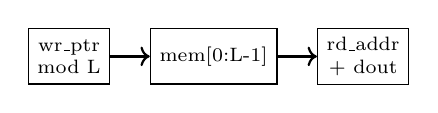
\begin{tikzpicture}[box/.style={draw,align=center,font=\scriptsize,minimum height=7mm}, node distance=5mm]
\node[box] (ptr) {wr\_ptr\\mod L};
\node[box, right=of ptr] (mem) {mem[0:L-1]};
\node[box, right=of mem] (rd) {rd\_addr\\+ dout};
\draw[->,thick] (ptr)--(mem); \draw[->,thick] (mem)--(rd);
\end{tikzpicture}
\caption{RTL: con trỏ ghi, mảng/M10K, đọc tuần tự.}
\end{figure}

\begin{verbatim}
localparam int L = 640;
reg signed [15:0] mem [0:L-1];
reg [\\$clog2(L)-1:0] wr_ptr, rd_ptr;
reg signed [15:0] dout;
always @(posedge clk) begin
  if (valid_i) begin
    mem[wr_ptr] <= din;            // Port A
    wr_ptr <= (wr_ptr == L-1) ? 0 : wr_ptr + 1'b1;
  end
  if (rd_en) begin
    dout <= mem[rd_ptr];           // Port B, Old Data
    rd_ptr <= (rd_ptr == L-1) ? 0 : rd_ptr + 1'b1;
  end
end
\end{verbatim}

\noindent\textbf{CẢNH BÁO --- read latency inferred vs IP.}
Đoạn mã \emph{inferred} RAM ở trên (\texttt{dout <= mem[rd\_ptr]}) tạo độ trễ đọc \textbf{1 chu kỳ} sau \texttt{rd\_en}.
Nếu instantiate M10K qua MegaWizard / On-Chip Memory IP (khuyến nghị mục~4): tùy chọn \textbf{Output Registers} bật $\Rightarrow$ thường \textbf{2 chu kỳ} (block RAM register + output register).
FSM Ch.11 và twin TB \textbf{phải} khớp đúng 1 hay 2 --- đếm sai một chu kỳ $\Rightarrow$ lệch mẫu cả khung.

\subsection*{Chi phí silicon --- giải thích từng mục}
\begin{costbox}
\textbf{Ngân sách silicon --- giải thích từng mục.}
\begin{itemize}[leftmargin=1.2em]
\item M10K: 1 khối cho $L=640\times16$ bit ($\approx10$\,kb); không dùng MLAB vì depth lớn.
\item ALM: con trỏ modulo + FSM đọc --- vài chục đến $\sim100$ ALM.
\item DSP: 0 (chỉ RAM).
\item Latency đọc: 1 ck (inferred) hoặc 2 ck (output register) --- phải khớp twin.
\item Vì sao True Dual-Port + Old Data: ghi và đọc song song mỗi chu kỳ audio; New Data không bảo đảm trên Cyclone~V mixed-port.
\end{itemize}

\noindent\textit{Tóm tắt số liệu:} Một khung $L=640$ mẫu $\times 16$~bit $=10\,240$~bit, vừa khít khoảng một khối \textbf{M10K} (còn dư vài trăm bit). Nếu làm tròn depth lên 1024 từ cho dễ địa chỉ, vẫn chỉ tốn 1--2 M10K. Khối này không dùng DSP. Số \textbf{ALM} cho hai con trỏ và FSM đọc thường khoảng 50--100. Đọc hết một khung cần $L$ chu kỳ cộng thêm \textbf{latency} đọc 1 hoặc 2 chu kỳ (tùy output register) --- con số này phải khớp Fmax và ngân sách thời gian thực 10\,ms/khung.
\end{costbox}

\subsection*{Bài tập + đáp án}


\begin{enumerate}\setlength{\itemsep}{2pt}
\item $L{=}640$, width 16: bao nhiêu bit? Cần mấy M10K tối thiểu?
\item Cùng addr R/W: Old Data trả gì?
\item Đọc frame khi \texttt{wr\_ptr}=100: addr đầu là bao nhiêu?
\end{enumerate}
\paragraph{Đáp án.} (1) $10240$ bit $\Rightarrow$ 1 M10K. (2) Giá trị trước ghi. (3) $(100)\bmod 640=100$ là ô mới nhất vừa tăng ptr --- oldest $=100$ nếu ptr đã tăng sau ghi; theo code trên sau ghi ptr đã +1 nên oldest $=\texttt{wr}$.
\subsection*{Ví dụ mở rộng, timing, Quartus, twin}

\begin{firstprin}{Circular buffer: mỗi địa chỉ là một mẫu theo thời gian cuốn}
Với $L=16$, ghi mẫu $1..20$: sau mẫu 20, 16 ô giữ $\{5..20\}$ theo thứ tự modulo (oldest$\to$newest tùy quy ước ptr). Đọc khung = $L$ địa chỉ liên tiếp modulo $L$ bắt đầu từ oldest. \textbf{Old Data:} cùng addr R/W trong một ck $\Rightarrow$ dout = giá trị trước ghi --- MegaWizard phải chọn đúng; twin trả old trong cùng delta-cycle.
\end{firstprin}

\noindent\textbf{Timing.} Inferred \texttt{dout <= mem[rd]}: latency 1 ck. IP Output Registers bật: thường 2 ck. FSM Ch.~11 và TB phải cùng model --- lệch 1 ck = lệch cả khung.

\noindent\textbf{Quartus.} On-Chip Memory 2-PORT; width 16; depth $\ge L$ (1024 ok); mixed-port RDW = Old Data; đừng dùng MLAB cho $L=640$.

\begin{verbatim}
L=640; mem=[0]*L; wr=0
def write(x):
    global wr
    old=mem[wr]; mem[wr]=int(x); wr=(wr+1)%L; return old
def read_frame():
    return [mem[(wr+k)%L] for k in range(L)]  # oldest-first if wr points next empty
\end{verbatim}

\begin{costbox}
\textbf{Chi tiết chip 5CSXFC6D6F31C6.} $640\times16=10240$ bit $\approx$ 1 M10K. Q2.30 depth 1024 $\Rightarrow\sim4$ M10K. ALM con trỏ $\sim50$--100. 0 DSP.
\end{costbox}

\subsection*{Thực hành --- Phiếu bài tập (mỗi phiếu chỉ ở đây)}

\subsubsection*{Phiếu 15 --- M10K RDW}

\textbf{Câu hỏi:} Nếu cắt/sai khối ``M10K RDW, hiện tượng nào phá $F_0$?
\begin{itemize}\setlength{\itemsep}{1pt}
\item \textbf{Vật lý:} Đọc nhầm New Data.
\item \textbf{Toán neo:} Old Data only.
\item \textbf{Silicon:} M10K.
\item \textbf{Pytest:} sim conflict test.
\item Tự làm: ví dụ tính tay 4--8 mẫu + điền bảng E$^\star$.
\end{itemize}

\clearpage
\phantomsection
\section*{Chương 6. Cửa sổ Hanning ROM $\times$ mẫu (Q1.15)}
\addcontentsline{toc}{section}{Chương 6. Cửa sổ Hanning ROM × mẫu (Q1.15)}
\pdfbookmark[1]{Chương 6. Cửa sổ Hanning ROM × mẫu}{chuong6}

\begin{learningobj}
Sau chương này bạn giải thích được vì sao khung âm thanh phải nhân cửa sổ Hanning trước khi tự tương quan; viết đúng công thức Praat ($N{+}1$) và đối chiếu dạng cổ điển ($N{-}1$); lượng tử hóa hệ số sang định dạng Q1.15; sinh tệp \texttt{hanning\_rom.hex} khớp bit với twin Python; hiện thực phép nhân ROM$\times$mẫu bằng một khối DSP trên Cyclone~V; và đọc được ngân sách M10K / DSP / ALM của khối cửa sổ.
\end{learningobj}

\subsection*{6.1. Hiện tượng thật: cắt khung không được ``cắt đứt'' sóng}

Giọng nói là một dòng sóng liên tục. Để đo chu kỳ rung dây thanh $T_0$, ta chỉ lấy một đoạn ngắn khoảng $40\,\text{ms}$ ($L = 640$ mẫu ở tần số lấy mẫu $f_s = 16\,\text{kHz}$), đúng như bản đồ khối ở Chương~0 đã ghi. Nếu lấy đoạn đó đúng kiểu cắt bằng kéo --- giữ nguyên biên độ đến mẫu cuối rồi nhảy đột ngột về 0 --- thì đoạn đó, nhìn từ miền tần số, giống một xung chữ nhật nhân với tín hiệu thật. Phép nhân trong miền thời gian tương đương \textbf{tích chập (convolution)} phổ tín hiệu với phổ của xung chữ nhật. Phổ xung chữ nhật là hàm $\mathrm{sinc}$: có một \textbf{thùy chính (mainlobe)} rộng và nhiều \textbf{thùy phụ (sidelobe)} cao khoảng $-13\,\text{dB}$ so với đỉnh (Chương~0 đã đổi $-13\,\text{dB}$ sang tỷ số biên độ $\approx 0{,}224$). Năng lượng ``rò'' qua các thùy phụ gọi là \textbf{rò phổ (spectral leakage)}.

Hệ quả với cao độ: đỉnh tự tương quan $\mathcal{R}_x[\tau]$ bị méo vì năng lượng giả từ các tần số láng giềng tràn sang đúng vùng tìm $F_0$ ($75 \ldots 600\,\text{Hz}$). Trực giác đời thường: bạn đang nghe một nốt đàn sạch, nhưng mỗi lần cắt đoạn lại ``vỗ'' hai đầu đoạn --- tiếng vỗ đó tạo thêm tiếng lách cách phổ, không có trong bản gốc.

Cửa sổ \textbf{Hanning} làm hai đầu khung về gần 0 một cách mượt, giống vuốt dần biên độ thay vì cắt đứt. Phổ Hanning có thùy phụ khoảng $-32\,\text{dB}$ (biên độ còn khoảng $1/40$ so với thùy chính, Chương~0). Thùy chính rộng hơn một chút (độ phân giải tần số kém hơn một ít), nhưng với bài đo $F_0$ bằng tự tương quan thời gian thì đánh đổi này rất đáng: ta cần đỉnh $\mathcal{R}_x$ sạch hơn là phổ sắc như dao.

\begin{physicalinsight}
Nhân cửa sổ $x[n]\cdot w[n]$ trên silicon chỉ là một phép nhân mỗi mẫu. Toàn bộ ``phép màu'' giảm rò phổ đã được nướng sẵn vào bảng hệ số $w[n]$. Không cần CORDIC, không cần sinh $\cos$ lúc chạy.
\end{physicalinsight}

\begin{figure}[H]
\centering
\begin{tikzpicture}[font=\small, >=Stealth]
  \draw[->] (0,0)--(8.2,0) node[right]{$n$};
  \draw[->] (0,0)--(0,2.8) node[above]{$w[n]$};
  \draw[thick, gray!70] (0.3,2.2)--(7.5,2.2) node[right,font=\scriptsize]{chữ nhật};
  \draw[thick, teal] (0.3,0)
    .. controls (1.5,0.15) and (2.2,2.2) .. (4.0,2.35)
    .. controls (5.8,2.2) and (6.5,0.15) .. (7.5,0);
  \node[teal, font=\scriptsize] at (4.0,2.6){Hanning};
  \draw[dashed, red!60] (0.3,0)--(0.3,2.2);
  \draw[dashed, red!60] (7.5,0)--(7.5,2.2);
  \node[red!70, font=\scriptsize, align=center] at (1.2,1.1){cắt đột\\gây rò phổ};
\end{tikzpicture}
\caption{Cửa sổ chữ nhật giữ biên độ đến sát biên rồi cắt đứt; Hanning vuốt hai đầu về 0, hạ thùy phụ từ khoảng $-13\,\text{dB}$ xuống khoảng $-32\,\text{dB}$.}
\label{fig:ch06_hanning_shape}
\end{figure}

\subsection*{6.2. Toán từng bước --- mọi ký hiệu trước khi dùng}

Gọi $L$ (hoặc $N$) là số mẫu trong một khung phân tích. Với sàn cao độ $75\,\text{Hz}$ ở $f_s = 16\,\text{kHz}$, Praat chọn khung dài khoảng ba chu kỳ: $L = 640$. Sau khi đã trừ mean cục bộ (Chương~3), tín hiệu cửa sổ là
\[
\tilde{x}[n] = (x[n] - \mu)\, w[n], \qquad n = 0,1,\ldots,L-1.
\]
Hai định nghĩa Hanning hay gặp --- phải chọn một và ghi vào twin:

\begin{enumerate}[leftmargin=1.4em]
\item \textbf{Praat ($N{+}1$), dùng trong golden \texttt{lab\_1\_3\_5.py}:}
\[
w[i] = 0{,}5 - 0{,}5\cos\Bigl(\frac{2\pi i}{N+1}\Bigr), \qquad i = 1,2,\ldots,N.
\]
Hai đầu lớn hơn 0 một chút (không đúng bằng 0). Với $N = 640$, mẫu số là $641$.
\item \textbf{Cổ điển / scipy ($N{-}1$):}
\[
w[n] = \frac12\Bigl(1 - \cos\frac{2\pi n}{N-1}\Bigr), \qquad n = 0,1,\ldots,N-1.
\]
Hai đầu đúng bằng 0; đối xứng $w[n] = w[N-1-n]$ sạch --- tiện lưu nửa bảng ROM.
\end{enumerate}

Gói FPGA này lấy dạng \textbf{Praat $N{+}1$} làm hợp đồng bit-exact với \texttt{hanning\_rom.hex} (đầy đủ 640 từ). Dạng cổ điển chỉ dùng trong ví dụ tính tay nhỏ và khi muốn minh họa tối ưu nửa bảng.

Lượng tử \textbf{Q1.15} (đã định nghĩa ở Chương~0: một bit dấu/phần nguyên, 15 bit phần thập phân; giá trị $1{,}0$ ánh xạ thành $2^{15} = 32768$, nhưng số có dấu 16-bit bão hòa tại $+32767$):
\[
w_q[n] = \mathrm{sat}_{16}\!\bigl(\mathrm{round}(w[n]\cdot 32768)\bigr) \in [0,32767]
\]
(với hệ số Hanning không âm). Mẫu vào $x_q$ cũng Q1.15. Tích rồi kéo về Q1.15 bằng làm tròn gần nhất:
\begin{align*}
y_{\mathrm{acc}} &= x_q \cdot w_q &&\text{(Q2.30, 32-bit có dấu)},\\
y_q &= \mathrm{sat}_{16}\!\bigl((y_{\mathrm{acc}} + 2^{14}) \ggg 15\bigr).
\end{align*}
Cộng $2^{14} = 16384$ trước khi dịch phải 15 bit chính là round-to-nearest trên số học hai's complement khi dùng arithmetic shift.

Năng lượng cửa sổ (dùng ở Chương~8 để chuẩn hóa):
\[
\mathcal{R}_w[0] = \sum_{n=0}^{N-1} w_q[n]^2
\]
tính offline trên int64; twin in giá trị này vào header hex để đối chiếu.

\subsection*{6.3. Ví dụ tính tay --- mọi số đã chạy Python}

Mọi con số dưới đây được kiểm chứng bởi \texttt{verify/verify\_chuong\_06\_09.py}.

\paragraph{A. Dạng cổ điển $N=8$ (đối xứng nửa bảng).}
$w[n] = \tfrac12\bigl(1 - \cos(2\pi n/7)\bigr)$, $n = 0..7$, lượng tử bằng $\mathrm{round}(w\cdot 32767)$ để minh họa hệ số dương:
\begin{center}\small
\begin{tabular}{@{}rrl@{}}\toprule
$n$ & $w[n]$ float & $w_q$ \\
\midrule
0 & 0.000000 & 0 \\
1 & 0.188255 & 6169 \\
2 & 0.611260 & 20029 \\
3 & 0.950484 & 31145 \\
\bottomrule
\end{tabular}
\end{center}
Đối xứng: $w_q[7] = w_q[0]$, $w_q[6] = w_q[1]$, \ldots --- ROM vật lý chỉ cần 4 từ. Nhân: $x_q = 10000$, $w_q = 20029$ cho tích $200\,290\,000$; làm tròn $({\rm acc}+2^{14})\ggg 15 = 6112$. Đối chiếu float $10000\times 0{,}611260 = 6112{,}6$ --- khớp trong 1 LSB.

\paragraph{B. Dạng Praat $N=8$ (khớp tinh thần golden).}
$w[i] = 0{,}5 - 0{,}5\cos(2\pi i/9)$, $i = 1..8$, lượng tử $\mathrm{round}(w\cdot 32768)$ rồi bão hòa:
\begin{center}\small
\begin{tabular}{@{}rrl@{}}\toprule
$i$ & $w$ float & $w_q$ \\
\midrule
1 & 0.116978 & 3833 \\
2 & 0.413176 & 13539 \\
3 & 0.750000 & 24576 \\
4 & 0.969846 & 31780 \\
\bottomrule
\end{tabular}
\end{center}
Hai đầu không về 0 tuyệt đối --- đúng hành vi Praat.

\paragraph{C. Khung thật $N=640$ Praat.}
Các mốc Q1.15: $w_q[0] = 1$, $w_q[1] = 3$, $w_q[319] = w_q[320] = 32767$, $w_q[638] = 3$, $w_q[639] = 1$. Tổng bình phương $\mathcal{R}_w[0] = \sum w_q^2 = 258\,100\,276\,868$ (int64).

\subsection*{6.4. Ý nghĩa phần cứng --- ROM On-Chip Memory + DSP}

Cửa sổ Hanning \emph{không} cần FIR Compiler~II: hệ số bất biến với $L$ cố định. Chọn IP \textbf{On-Chip Memory} kiểu ROM (hoặc RAM 1-PORT khởi tạo \texttt{.hex}/\texttt{.mif}):
\begin{itemize}[leftmargin=1.4em]
\item Width $= 16$ (Q1.15), depth $= 640$ (đầy đủ, khớp Praat) hoặc $320$ nếu dùng dạng cổ điển nửa bảng.
\item Registered output: 1 chu kỳ đọc --- FSM phải chờ đúng latency này.
\item Một khối \textbf{DSP} (\emph{Digital Signal Processing} block) trên Cyclone~V nhân $18\times 19$ mỗi mẫu: $x_q\times w_q$.
\end{itemize}
Không gọi FIR Compiler chỉ để nhân cửa sổ: lãng phí logic cấu hình systolic. Đổi $L$ hoặc công thức $w$ thì \textbf{bắt buộc rebuild hex} và nạp lại ROM; quên bước này thì $F_0$ sai im lặng.

\paragraph{RTL datapath --- giải thích từng dòng.}
\begin{verbatim}
module window_hanning #(
  parameter N = 640
)(
  input  wire               clk, rst_n,
  input  wire               in_valid,
  output wire               in_ready,
  input  wire signed [15:0] x_q,        // Q1.15
  output reg                out_valid,
  input  wire               out_ready,
  output reg  signed [15:0] y_q         // Q1.15 windowed
);
  (* ram_init_file = "hanning_rom.hex" *)
  reg [15:0] rom [0:N-1];
  reg [9:0]  n;                         // 0..N-1
  wire signed [15:0] w_q = rom[n];
  wire signed [31:0] prod = x_q * w_q;  // Q2.30
  wire signed [31:0] rounded = prod + 32'sd16384;
  wire signed [31:0] shifted = rounded >>> 15;
  function automatic signed [15:0] sat16;
    input signed [31:0] v;
    begin
      if (v > 32'sd32767) sat16 = 16'sd32767;
      else if (v < -32'sd32768) sat16 = -16'sd32768;
      else sat16 = v[15:0];
    end
  endfunction
  assign in_ready = out_ready | ~out_valid;
  always @(posedge clk or negedge rst_n) begin
    if (!rst_n) begin n <= 0; out_valid <= 0; y_q <= 0; end
    else if (in_valid && in_ready) begin
      y_q <= sat16(shifted);
      out_valid <= 1'b1;
      n <= (n == N-1) ? 10'd0 : n + 10'd1;
    end else if (out_valid && out_ready) out_valid <= 1'b0;
  end
endmodule
\end{verbatim}
\texttt{in\_ready}/\texttt{out\_ready} là handshake Avalon-ST (sink/source, Chương~0): khi downstream chưa sẵn sàng, upstream phải giữ \texttt{valid}. Hàm \texttt{sat16} bão hòa thay vì wrap, tránh đảo dấu khi tích lớn.

Nếu muốn tiết kiệm một nửa BRAM với dạng cổ điển: địa chỉ \texttt{(n < 320) ? n : (639-n)} và ROM depth 320. Twin phải cùng công thức --- không trộn Praat hex với địa chỉ nửa bảng cổ điển.

\subsection*{6.5. Twin Python bit-exact}

\begin{verbatim}
import numpy as np
Q15 = 1 << 15

def hanning_praat_q15(N=640):
    i = np.arange(1, N + 1, dtype=np.float64)
    w = 0.5 - 0.5 * np.cos(2.0 * np.pi * i / (N + 1))
    return np.clip(np.round(w * Q15), 0, Q15 - 1).astype(np.int64)

def apply_window(xq, wq):
    prod = xq.astype(np.int64) * wq.astype(np.int64)
    return ((prod + (1 << 14)) >> 15).astype(np.int64)

wq = hanning_praat_q15(640)
with open("hex/hanning_rom.hex", "w") as f:
    for v in wq:
        f.write(f"{int(v) & 0xFFFF:04X}\n")
print("Rw0 =", int(np.sum(wq * wq)))
\end{verbatim}
Mọi thay đổi round/sat phải sửa \textbf{cùng chỗ} RTL và twin --- đó là hợp đồng bit-exact. Script kiểm số tay: \texttt{verify/verify\_chuong\_06\_09.py}.

\subsection*{6.6. Chi phí silicon --- viết tắt mở rộng lần đầu trong chương}

\begin{costbox}
\textbf{Ngân sách khối cửa sổ.}
\begin{itemize}[leftmargin=1.2em]
\item \textbf{M10K} (khối BRAM nhúng $10\,240$ bit trên Cyclone~V, Chương~0): ROM đầy đủ $640\times 16 = 10\,240$\,bit $=$ đúng 1 M10K. Nửa bảng cổ điển $320\times 16 = 5\,120$\,bit vẫn chiếm 1 M10K (không chia nhỏ hơn một block).
\item \textbf{DSP}: 1 nhân $18\times 19$ mỗi mẫu cửa sổ (có thể dùng chung với MAC ở Pha~2 nếu FSM tuần tự).
\item \textbf{ALM} (\emph{Adaptive Logic Module} --- đơn vị logic cơ bản Cyclone~V, gồm LUT look-up table + flip-flop): con trỏ $n$ + sat + handshake $\lesssim 80$ ALM.
\item \textbf{Fmax} (tần số đồng hồ tối đa sau place-and-route): $\gg 50\,\text{MHz}$ --- đường nhân một chu kỳ không phải nút thắt.
\item \textbf{Latency}: 1 chu kỳ đọc ROM (cộng 0/1 chu kỳ nhân pipeline tùy suy diễn).
\item Vì sao ROM chứ không CORDIC: $w[n]$ bất biến; tính offline một lần rẻ hơn sinh $\cos$ lúc chạy hàng nghìn lần mỗi giây.
\end{itemize}
\end{costbox}

\subsection*{6.7. Bài tập và lời giải giải thích}

\paragraph{Bài tập 6.1.} Sinh hex Praat $N=8$; đối chiếu bốn từ đầu với bảng mục 6.3.B.

\paragraph{Bài tập 6.2.} RTL sim: khung toàn mẫu $32767$ nhân Hanning --- mô tả biên độ $y$ ở hai đầu và giữa khung. Giải thích vì sao.

\paragraph{Bài tập 6.3.} Cố ý dùng hex Praat nhưng địa chỉ nửa bảng cổ điển: $\mathcal{R}_x[\tau]$ lệch twin thế nào?

\paragraph{Bài tập 6.4.} Tính tay $x_q = -10000$, $w_q = 20029$ với cùng quy tắc $+16384$ rồi $\ggg 15$. Kết quả?

\noindent\textbf{Lời giải giải thích.}
\begin{enumerate}[leftmargin=1.4em]
\item Kỳ vọng bốn từ đầu $3833$, $13539$, $24576$, $31780$ (script đã assert).
\item Giữa khung $w\approx 1$ nên $y\approx 32767$; hai đầu $w$ nhỏ nên $y$ nhỏ --- đúng hình quả núi Hanning. Đây là hệ quả trực tiếp của công thức Praat, không phải lỗi bão hòa.
\item Hệ số sai đối xứng làm méo $\mathcal{R}_x$, đỉnh $\tau$ lệch vài mẫu, dẫn đến sai vài chục cent khi đối chiếu Praat ở Chương~13.
\item Tích $-200\,290\,000$; cộng $16384$ rồi arithmetic $\ggg 15$ cho $-6112$ (đối xứng với ví dụ dương ở mục 6.3.A). Script xác nhận \texttt{q15\_mul(-10000, 20029) == -6112}.
\end{enumerate}

\clearpage
\phantomsection
\section*{Chương 7. Tự tương quan --- MAC mặc định / FFT tùy chọn + BFP}
\addcontentsline{toc}{section}{Chương 7. Tự tương quan — MAC mặc định / FFT tùy chọn + BFP}
\pdfbookmark[1]{Chương 7. Tự tương quan — MAC mặc định / FFT tùy chọn + BFP}{chuong7}

\begin{learningobj}
Sau chương này bạn viết được định nghĩa tự tương quan không vòng từ nguyên lý đầu tiên; tính tay từng giá trị $\mathcal{R}[\tau]$ trên chuỗi ngắn và trên khung cosin chu kỳ~8; thiết kế datapath MAC tuần tự bằng một khối DSP và bộ tích lũy rộng kèm bảng timing chu kỳ; giải thích FFT IP radix-4 / BFP từng tầng cánh bướm và barrel shift $2^{2e}$ trước IFFT; viết twin Python bit-exact; và tính được ngân sách chu kỳ / RTF so với bước nhảy $10\,\text{ms}$.
\end{learningobj}

\subsection*{7.1. Hiện tượng thật: đo mức ``giống chính mình''}

Khi dây thanh quản rung gần tuần hoàn với chu kỳ cơ bản $T_0$ giây, sóng áp suất tại thời điểm $t$ gần trùng với sóng tại $t+T_0$. Trên lưới mẫu $f_s = 16\,\text{kHz}$, chu kỳ đó là $\tau_0 = f_s\cdot T_0$ mẫu. Ví dụ giọng nam khoảng $100\,\text{Hz}$ cho $\tau_0 = 160$; giọng nữ khoảng $200\,\text{Hz}$ cho $\tau_0 = 80$. Phép \textbf{tự tương quan (autocorrelation)} đo mức giống nhau đó bằng cách trượt một bản sao đi $\tau$ mẫu (\textbf{độ trễ --- lag}), nhân từng cặp mẫu chồng nhau và cộng dồn. Tại $\tau = \tau_0$, các cặp cùng pha cho tích dương lớn, tạo đỉnh nổi trên đồ thị $\mathcal{R}_x[\tau]$. Đo được $\tau_0$ thì suy ra ngay $F_0 = f_s/\tau_0$.

Đây là hiện tượng vật lý thật của sóng tuần hoàn, không chỉ là quy ước toán học. Định lý \textbf{Wiener--Khinchin} (Chương~0) chứng minh rằng $\mathcal{R}_x$ cũng bằng biến đổi Fourier ngược của mật độ phổ công suất $|X[k]|^2$, nên có hai đường silicon tương đương về toán: nhân--cộng trực tiếp (MAC) hoặc FFT $\to |X|^2 \to$ IFFT. Với dải trễ hẹp $\tau = 26 \ldots 214$ (189 giá trị, khớp \texttt{lab\_1\_3\_5.py} và bản đồ Chương~0), đường mặc định trên Cyclone~V là \textbf{MAC} (\emph{Multiply-ACcumulate}): chỉ tính đúng những $\tau$ cần thiết, không tính toàn bộ phổ rồi mới cắt. Mỗi hop $10\,\text{ms}$ chỉ có $500\,000$ chu kỳ ở $50\,\text{MHz}$; $98\,280$ phép MAC chiếm khoảng một phần năm ngân sách đó và vẫn để lại biên cho cửa sổ, chuẩn hóa và chia $F_0$.

Tại sao không lấy đỉnh phổ trực tiếp? Vì phổ biên độ của nguyên âm có đỉnh formant (cộng hưởng ống thanh) có thể cao hơn đỉnh $F_0$; tự tương quan thời gian ``nhìn'' chu kỳ lặp của toàn sóng, ít bị formant đánh lừa hơn --- đó là lý do Praat chọn ACF (sau chuẩn hóa) làm lõi đo cao độ.

\begin{physicalinsight}
Tự tương quan không ``tạo ra'' cao độ. Nó chỉ đo độ trùng pha giữa tín hiệu và bản sao trễ của chính nó. Nếu khung đã bị rò phổ hoặc còn DC (Chương~3,~6), đỉnh giả sẽ cạnh tranh với đỉnh thật --- MAC tính đúng công thức vẫn báo sai $F_0$.
\end{physicalinsight}

\begin{figure}[H]
\centering
\begin{tikzpicture}[font=\small, >=Stealth]
  \draw[->] (0,0)--(9.0,0) node[right]{$\tau$ (mẫu)};
  \draw[->] (0,0)--(0,3.0) node[above]{$\mathcal{R}_x[\tau]$};
  \draw[thick, teal] (0.3,2.7)--(1.2,0.9)--(2.4,2.2)--(3.6,0.7)--(4.8,1.6)--(6.0,0.5)--(7.2,1.1)--(8.4,0.4);
  \fill[red!70] (2.4,2.2) circle (2.2pt) node[above right,font=\scriptsize]{$\tau_0=T_0$};
  \fill[orange!80] (4.8,1.6) circle (2.2pt) node[above,font=\scriptsize]{$2T_0$};
  \node[font=\scriptsize, align=left] at (7.0,2.4){đỉnh phụ bội\\có thể gây sai quãng tám};
\end{tikzpicture}
\caption{Hàm tự tương quan của khung hữu thanh: đỉnh toàn cục tại $\tau=0$ (năng lượng), đỉnh cục bộ đầu tiên tại $\tau_0=T_0$ là ứng viên cao độ; đỉnh $2T_0$ là ứng viên sai quãng tám.}
\label{fig:ch07_acf_peaks}
\end{figure}

\subsection*{7.2. Toán từng bước --- định nghĩa gốc trước mọi phím tắt}

Hàm tự tương quan \textbf{không vòng (linear / non-circular)} của khung $x[n]$ độ dài $L$ được định nghĩa từ tích vô hướng của hai đoạn chồng:
\[
\mathcal{R}_x[\tau] = \sum_{n=0}^{L-1-\tau} x[n]\cdot x[n+\tau], \qquad \tau \ge 0.
\]
Từng bước: (1)~chọn $\tau$; (2)~lấy cặp $(x[0],x[\tau])$, $(x[1],x[\tau+1])$, \ldots, $(x[L-1-\tau],x[L-1])$; (3)~nhân từng cặp; (4)~cộng tất cả tích. Không được viết tắt thành ``chỉ một hạng $x[0]x[\tau]$''.

Mỗi ký hiệu:
\begin{itemize}[leftmargin=1.4em]
\item $x[n]$: mẫu đã trừ mean và đã nhân cửa sổ Hanning (Chương~3,~6), định dạng Q1.15 trên silicon.
\item $\tau$: độ trễ tính bằng số mẫu. Dải quét phần cứng: $\tau \in [26,214]$ (189 giá trị) để đỉnh tìm trong $[27,213]$ luôn có láng giềng cho nội suy parabolic (Chương~9). Sàn $75\,\text{Hz}$ $\leftrightarrow$ $\tau\approx 213$; trần $600\,\text{Hz}$ $\leftrightarrow$ $\tau\approx 27$.
\item Số hạng trong tổng đúng bằng $L-\tau$: trễ càng lớn, càng ít cặp chồng --- đây là thiên vị hình học sẽ được bù ở Chương~8.
\item Tại $\tau=0$: $\mathcal{R}_x[0] = \sum_n x[n]^2$ là năng lượng khung (cực đại toàn cục).
\end{itemize}

Định lý Wiener--Khinchin cho phép đường tương đương:
\[
\mathcal{R}_x[\tau] = \mathcal{F}^{-1}\{|X[k]|^2\}.
\]
FFT mặc định tính tự tương quan \textbf{vòng (circular)}: mẫu cuối ``quấn'' sang mẫu đầu. Muốn khớp định nghĩa không vòng ở trên phải zero-pad ít nhất thêm $L$ số 0 trước FFT (thường pad lên $N_{\mathrm{FFT}}=1024$ hoặc $2048$). Đó là một trong những lý do đường mặc định pitch chọn MAC.

Trên silicon, mỗi tích $x[n]\cdot x[n+\tau]$ là Q1.15$\times$Q1.15 $=$ Q2.30 (32-bit). Cộng dồn đến $640$ hạng tử đòi hỏi bộ tích lũy rộng: thiết kế dùng \textbf{41-bit có dấu} (khớp stub \texttt{rtl/mac\_autocorr.v} và comment trong \texttt{lab\_1\_3\_5.py}). Ước lượng thô: $|x|\le 2^{15}$, $|x\cdot x|\le 2^{30}$, $640\cdot 2^{30} < 2^{40}$ --- 41 bit có dấu vừa đủ biên an toàn một bit.

\subsection*{7.3. Ví dụ tính tay --- mọi số đã chạy Python}

\paragraph{A. Chuỗi cực ngắn $x = [1,2,1,2]$.}
Từng cặp:
\begin{align*}
\mathcal{R}[0] &= 1\cdot 1 + 2\cdot 2 + 1\cdot 1 + 2\cdot 2 = 1+4+1+4 = 10,\\
\mathcal{R}[1] &= 1\cdot 2 + 2\cdot 1 + 1\cdot 2 = 2+2+2 = 6,\\
\mathcal{R}[2] &= 1\cdot 1 + 2\cdot 2 = 1+4 = 5,\\
\mathcal{R}[3] &= 1\cdot 2 = 2.
\end{align*}
Tỉ số thô $\mathcal{R}[2]/\mathcal{R}[0] = 0{,}5$. Sau khi nhân $C[\tau]$ (Chương~8) và chia theo số hạng, đỉnh chu kỳ được kéo về gần 1.

\paragraph{B. Khung cosin chu kỳ 8 mẫu, $N=16$ (Q1.15).}
$x[n] = \mathrm{sat}_{16}(\mathrm{round}(\cos(2\pi n/8)\cdot 32768))$, $n=0..15$. Từng bước cho $n=0$: $\cos 0 = 1$, $\mathrm{round}(32768)=32768$, sat $\to 32767$. Cho $n=4$: $\cos\pi = -1$, $\mathrm{round}(-32768)=-32768$ (vừa khít min int16).
\begin{center}\footnotesize
\begin{tabular}{@{}lllllllll@{}}\toprule
$n$ & 0 & 1 & 2 & 3 & 4 & 5 & 6 & 7 \\
$x$ & 32767 & 23170 & 0 & $-23170$ & $-32768$ & $-23170$ & 0 & 23170 \\
\midrule
$n$ & 8 & 9 & 10 & 11 & 12 & 13 & 14 & 15 \\
$x$ & 32767 & 23170 & 0 & $-23170$ & $-32768$ & $-23170$ & 0 & 23170 \\
\bottomrule
\end{tabular}
\end{center}
Tự tương quan không vòng (script):
\begin{align*}
\mathcal{R}[0] &= 8\,589\,627\,426,\\
\mathcal{R}[8] &= 4\,294\,813\,713 \approx \tfrac12\mathcal{R}[0],\\
\mathcal{R}[4] &= -6\,442\,220\,568 \quad\text{(chống pha, không phải đỉnh dương)}.
\end{align*}
Tỉ số thô $\mathcal{R}[8]/\mathcal{R}[0] = 0{,}5$ vì chỉ còn 8 cặp; sau chuẩn hóa unbiased $(\mathcal{R}[8]/8)/(\mathcal{R}[0]/16) = 1$. Đây là lý do Chương~8 tồn tại.

\paragraph{C. Ngân sách chu kỳ trên đường MAC thật.}
Với $\tau = 26\ldots 214$, tổng số phép nhân--cộng đúng bằng
\[
N_{\mathrm{MAC}} = \sum_{\tau=26}^{214}(640-\tau).
\]
Tính tổng cấp số: số hạng $189$; số hạng đầu $640-26=614$; số hạng cuối $640-214=426$; tổng $= 189\cdot(614+426)/2 = 98\,280$.
Không phải $189\times 640 = 120\,960$ --- công thức naïve đếm thừa. Tại $f_{\mathrm{clk}} = 50\,\text{MHz}$:
\[
T_{\mathrm{compute}} = \frac{98\,280}{50\times 10^6} = 1{,}9656\,\text{ms}, \qquad
\mathrm{RTF} = \frac{1{,}9656}{10} = 0{,}19656 \ll 1.
\]

\subsection*{7.4. Ý nghĩa phần cứng --- MAC mặc định}

Hai con trỏ đọc khung trong BRAM True Dual-Port (Chương~5): một trỏ tới $x[n]$, một tới $x[n+\tau]$. Mỗi chu kỳ một khối DSP nhân $18\times 18$ (hoặc $18\times 19$), cộng vào bộ tích lũy 41-bit có dấu. Quét $\tau$ tuần tự. Sau $(L-\tau)$ bước, thanh ghi accum chính là $\mathcal{R}_x[\tau]$.

\begin{figure}[H]
\centering
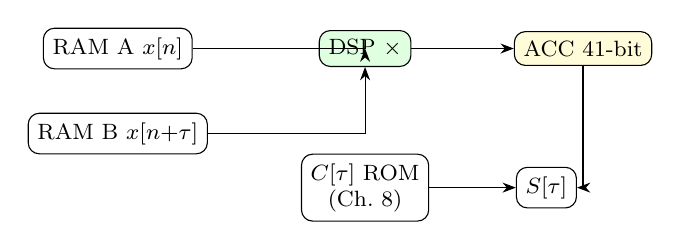
\begin{tikzpicture}[font=\footnotesize, >=Stealth]
  \node[draw, rounded corners] (a) {RAM A $x[n]$};
  \node[draw, rounded corners, below=0.55cm of a] (b) {RAM B $x[n{+}\tau]$};
  \node[draw, rounded corners, fill=green!12, right=1.6cm of a] (m) {DSP $\times$};
  \node[draw, rounded corners, fill=yellow!15, right=1.3cm of m] (acc) {ACC 41-bit};
  \draw[->] (a) -| (m); \draw[->] (b) -| (m); \draw[->] (m) -- (acc);
  \node[draw, rounded corners, below=1.1cm of m, align=center] (rom) {$C[\tau]$ ROM\\(Ch.~8)};
  \node[draw, rounded corners, right=1.1cm of rom] (s) {$S[\tau]$};
  \draw[->] (acc) |- (s); \draw[->] (rom) -- (s);
\end{tikzpicture}
\caption{Datapath MAC: hai toán hạng từ TDP RAM, một nhân DSP, một tích lũy --- khớp vòng \texttt{for tau} trong \texttt{lab\_1\_3\_5.py}.}
\label{fig:ch07_mac_datapath}
\end{figure}

\paragraph{Bảng timing chu kỳ --- một $\tau$ cố định (ví dụ $\tau=2$, $L=4$).}
\begin{center}\small
\begin{tabular}{@{}cllll@{}}\toprule
ck & Trạng thái & $n$ & $xa{=}x[n]$, $xb{=}x[n{+}\tau]$ & \texttt{acc} sau cạnh \\
\midrule
0 & IDLE$\to$LOAD & --- & --- & clear $0$ \\
1 & RUN & 0 & $x[0],x[2]$ & $x[0]x[2]$ \\
2 & RUN & 1 & $x[1],x[3]$ & $x[0]x[2]+x[1]x[3]$ \\
3 & DONE & --- & --- & $=\mathcal{R}[2]$; \texttt{done\_tau}=1 \\
\bottomrule
\end{tabular}
\end{center}
Với $\tau=26$, $L=640$: pha RUN kéo dài đúng $614$ chu kỳ. FSM ngoài tăng $\tau$ và lặp. Không được clear \texttt{acc} giữa các $n$ của cùng một $\tau$.

\paragraph{RTL lõi (ý tưởng, khớp stub \texttt{mac\_autocorr.v}).}
\begin{verbatim}
module mac_autocorr (
  input  wire               clk, rst_n, start,
  input  wire signed [15:0] xa, xb,   // x[n], x[n+tau] Q1.15
  input  wire [9:0]         n_pairs,  // = L - tau
  output reg  signed [40:0] acc,      // 41-bit signed
  output reg                done_tau
);
  // FSM: IDLE -> RUN (n_pairs cycles: acc <= acc + xa*xb) -> DONE
  // xa, xb phải ổn định đúng cạnh khi acc cập nhật (đồng bộ với
  // latency đọc TDP RAM --- thường 1 ck registered).
endmodule
\end{verbatim}
Không dùng \texttt{numpy.correlate} float làm chuẩn silicon: twin phải nhân--cộng int cùng độ rộng accum.

\subsection*{7.5. Đường tùy chọn: FFT IP + BFP + barrel shift trước IFFT}

Chỉ bật sau khi MAC đã xanh bit-exact. Dùng \textbf{FFT Intel FPGA IP} (User Guide~683374):

\begin{itemize}[leftmargin=1.4em]
\item Kiến trúc \textbf{radix-4} (hoặc radix-2): mỗi tầng cánh bướm (\textbf{butterfly}) kết hợp 4 (hoặc 2) điểm với twiddle $W_N^k = e^{-j2\pi k/N}$ lấy từ ROM nội bộ. Với $N=1024$ radix-4 cần $\log_4 1024 = 5$ tầng; radix-2 cần 10 tầng.
\item Streaming hoặc buffered; tín hiệu SOP/EOP đánh dấu một block $N$ điểm trên Avalon-ST.
\item \textbf{Block Floating Point (BFP --- số chấm động khối)}: mọi bin chia sẻ một số mũ nguyên $e$; mantissa dịch sao cho $\max|m|$ vừa khít bit. Sau mỗi tầng butterfly, nếu có nguy cơ tràn thì toàn vector dịch phải 1 bit và $e$ tăng 1. IP xuất \texttt{source\_exp}.
\item BFP \textbf{không} có cổng nhập exponent vào IFFT --- kỹ sư phải scale bên ngoài trước khi đưa mantissa vào IFFT.
\end{itemize}

\paragraph{BFP từng tầng --- ví dụ mantissa 8-bit, 2 tầng.}
Bắt đầu stage~0: $m = [40,-30,10,-5]$, $e = 0$. Ngưỡng tràn minh họa $= 32$ (giả sử còn 1 bit đầu). Vì $\max|m| = 40 > 32$:
\begin{center}\small
\begin{tabular}{@{}clll@{}}\toprule
Sự kiện & $e$ & Mantissa & Ghi chú \\
\midrule
Vào stage 0 & 0 & $[40,-30,10,-5]$ & $\max=40>32$ \\
Sau scale stage 0 & 1 & $[20,-15,5,-2]$ & dịch phải 1 \\
Sau stage 1 (không tràn) & 1 & $[20,-15,5,-2]$ & giữ $e$ \\
Power bin 0 thô $|m|^2$ & --- & $400$ & quên $2^{2e}$ \\
Power đúng $|m|^2\cdot 2^{2e}$ & --- & $1600$ & $=40^2$ \\
\bottomrule
\end{tabular}
\end{center}

\begin{firstprin}{Sau $|X|^2$, số mũ nhân đôi thành $2e$}
Mantissa $y = 3$, exponent $e = 2$ có giá trị thật $3\cdot 2^{-2}$. Bình phương:
\[
(3\cdot 2^{-2})^2 = 9\cdot 2^{-4}
\]
--- số mũ thành $2e$. Đẩy mantissa $|y|^2$ thẳng vào IFFT (IP kỳ vọng fixed-point với exponent $=0$ ở lối vào) mà quên barrel-shift theo $2e$ sẽ làm cả dải động $\mathcal{R}[\tau]$ sai tỷ lệ, phá ngưỡng voicing.
\end{firstprin}

\paragraph{Barrel shift trước IFFT.}
RTL bắt buộc: nếu \texttt{source\_exp}$=e$ sau FFT, sau khi tính $|X[k]|^2$ trên mantissa, dịch trái (hoặc nhân) kết quả theo $2e$ trước khi đưa vào IFFT --- hoặc dịch mantissa IFFT input tương đương. Twin phải dùng model \texttt{\_model} của variation FFT IP, không đoán $e$.

\begin{figure}[H]
\centering
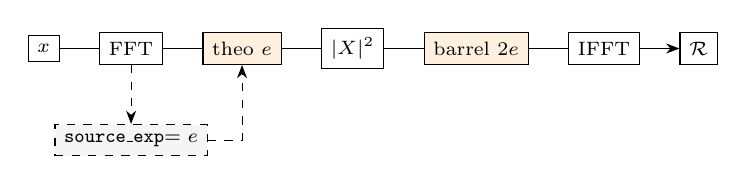
\begin{tikzpicture}[font=\scriptsize, >=Stealth]
  \node[draw] (x) {$x$};
  \node[draw, right=0.5cm of x] (fft) {FFT};
  \node[draw, fill=orange!12, right=0.5cm of fft] (sh1) {theo $e$};
  \node[draw, right=0.5cm of sh1] (mag) {$|X|^2$};
  \node[draw, fill=orange!12, right=0.5cm of mag] (sh2) {barrel $2e$};
  \node[draw, right=0.5cm of sh2] (ifft) {IFFT};
  \node[draw, right=0.5cm of ifft] (r) {$\mathcal{R}$};
  \draw[->] (x)--(fft)--(sh1)--(mag)--(sh2)--(ifft)--(r);
  \node[draw, dashed, below=0.75cm of fft, fill=gray!8] (exp) {\texttt{source\_exp}$=e$};
  \draw[->, dashed] (fft) -- (exp);
  \draw[->, dashed] (exp.east) -| (sh1.south);
\end{tikzpicture}
\caption{Đường FFT/Wiener--Khinchin: hai khối cam (scale theo $e$ và barrel $2^{2e}$) là RTL bắt buộc. Quên chúng gần như chắc fail bit-exact --- đó là lý do mặc định vẫn là MAC.}
\label{fig:ch07_fft_bfp}
\end{figure}

\paragraph{Vì sao MAC thắng khi $\tau_{\max}\ll L$.}
MAC: $98\,280$ nhân thực/khung. FFT 1024 radix-4: 5 tầng, mỗi tầng $256$ butterfly phức (mỗi butterfly vài nhân thực) --- cộng IFFT tương tự cộng $|X|^2$, rồi vẫn phải cắt $\tau$. Thêm rủi ro bit-reverse và BFP. Chỉ mở FFT khi lab yêu cầu so khớp đường Praat FFT hoặc khi RTF MAC không đủ.


\paragraph{Bit-reverse và thứ tự bin.}
FFT IP có thể xuất dữ liệu theo thứ tự bit-reverse hoặc natural order tùy cấu hình. Twin và RTL sau $|X|^2$ phải cùng thứ tự trước IFFT. Sai thứ tự bin làm $\mathcal{R}[\tau]$ ``xáo'' --- đỉnh $\tau_0$ có thể biến mất hoặc nhảy chỗ. Lab nghiệm thu nhánh FFT bắt buộc so dump toàn bộ $|X[k]|^2$ với model IP trước khi nối IFFT.

\paragraph{Zero-pad cụ thể.}
Khung $L=640$ pad thêm ít nhất 640 số 0 lên $N_{\mathrm{FFT}}=2048$ (hoặc 1024 nếu chấp nhận circular leak nhỏ và đã đo sai số). Pad ngắn hơn $2L-1$ làm tự tương quan vòng ``đụng'' đuôi vào đầu --- $\mathcal{R}[\tau]$ tại $\tau$ lớn bị cộng thêm hạng giả. MAC không bao giờ gặp lỗi này vì định nghĩa gốc chỉ cộng $L-\tau$ hạng thật.

Trên DE10-Standard, chọn MAC mặc định còn vì một lý do vận hành: khi debug cent-error ở Chương~13, kỹ sư chỉ cần so từng $\mathcal{R}[\tau]$ int với twin; không phải lần theo \texttt{source\_exp} từng block. FFT giữ trong tài liệu như đường tùy chọn để hiểu Wiener--Khinchin và để lab nâng cao so khớp Praat khi bật biến thể phổ.

\subsection*{7.6. Twin Python bit-exact}

\begin{verbatim}
import numpy as np

def acf_linear_int(x, tau_min, tau_max):
    x = np.asarray(x, dtype=np.int64)
    L = len(x)
    out = {}
    for tau in range(tau_min, tau_max + 1):
        # Khớp MAC: cộng dồn int, không float
        out[tau] = int(np.dot(x[: L - tau], x[tau:]))
    return out

# Khớp lab: tau 26..214, accum int64 (>= 41-bit signed trên RTL)
R = acf_linear_int(xw_q15, 26, 214)
# So dump R[tau] với ModelSim: sai lệch 0 bit trên đường MAC
\end{verbatim}
Giải thích: \texttt{np.dot} trên \texttt{int64} tương đương vòng RUN của FSM; không lấy \texttt{numpy.correlate} float. Trên nhánh FFT, twin phải gồm cả barrel $2^{2e}$ giống RTL và so với \texttt{\_model} của IP.


Khi đo RTF thực tế trên board, đừng chỉ đếm chu kỳ MAC lý thuyết: thêm latency đọc TDP RAM (1~ck/mẫu), handshake Avalon-ST có thể chen \texttt{waitrequest}, và pha nhân $C[\tau]$ (Chương~8). Ngân sách an toàn lab: dành $3\,\text{ms}$ cho toàn bộ Pha~2 (cửa sổ + MAC + chuẩn hóa + peak), tương đương RTF $0{,}3$. Nếu sau place-and-route Fmax tụt dưới $40\,\text{MHz}$, phải pipeline thêm nhân DSP hoặc giảm $\tau_{\max}$ --- không được ``hy vọng'' timing tự hết.

\subsection*{7.7. Chi phí silicon}

\begin{costbox}
\textbf{Ngân sách MAC autocorr (default).}
\begin{itemize}[leftmargin=1.2em]
\item \textbf{DSP}: 1 khối MAC/chu kỳ; $98\,280$ phép/khung $\approx 1{,}97\,\text{ms}$ @ $50\,\text{MHz}$.
\item \textbf{ALM}: $\sim 200$ cho FSM con trỏ $\tau$, $n$, handshake Avalon-ST.
\item \textbf{M10K}: đệm khung dùng chung Chương~5; MAC không thêm BRAM.
\item \textbf{RTF} $= 0{,}197 \ll 1$ (còn $>80\%$ thời gian rảnh mỗi hop $10\,\text{ms}$ $= 500\,000$ chu kỳ). Vì sao vừa khít: ngay cả khi thêm cửa sổ + $C[\tau]$ + parabolic + chia, tổng vẫn dưới khoảng $3\,\text{ms}$, RTF $<0{,}3$.
\item \textbf{FFT optional}: hàng nghìn ALM + nhiều M10K twiddle/buffer + DSP theo variation; barrel shifter vài chục ALM. Chỉ bật khi twin đã khóa và lab yêu cầu.
\item Vì sao MAC mặc định: 0 rủi ro BFP/bit-reverse, 0-bit với golden \texttt{lab\_1\_3\_5.py}.
\end{itemize}
\end{costbox}


Tóm lại: đường MAC là hợp đồng bit-exact mặc định của gói này; đường FFT/BFP là bài học kiến trúc và bài lab nâng cao. Mọi số trong mục 7.3 đã chạy qua \texttt{verify/verify\_chuong\_06\_09.py} --- nếu sửa công thức pad hoặc độ rộng accum, sửa script trước rồi mới sửa RTL.

\subsection*{7.8. Bài tập và lời giải giải thích}

\paragraph{Bài tập 7.1.} Với $x = [1,2,1,2]$, tính $\mathcal{R}[1]$ và $\mathcal{R}[2]$ từ định nghĩa gốc. Có được phép viết $\mathcal{R}[2] = x[0]x[2]$ một hạng duy nhất không?

\paragraph{Bài tập 7.2.} Trên khung cosin mục 7.3.B, vì sao $\mathcal{R}[8]/\mathcal{R}[0] = 0{,}5$ dù tín hiệu lặp hoàn hảo? Làm thế nào để tỉ số về gần 1?

\paragraph{Bài tập 7.3.} Mantissa sau FFT $m = 20$, $e = 1$. Tính power $|m|^2\cdot 2^{2e}$. Nếu quên nhân $2^{2e}$, sai bao nhiêu lần?

\paragraph{Bài tập 7.4.} Tính $N_{\mathrm{MAC}}$ đúng bằng $\sum_{\tau=26}^{214}(640-\tau)$ và RTF @ $50\,\text{MHz}$. So với ước lượng naïve $189\times 640$.

\paragraph{Bài tập 7.5.} Vẽ bảng timing 4 chu kỳ cho $\tau=1$, $L=4$, $x=[1,2,1,2]$: mỗi cạnh \texttt{acc} mang giá trị gì? \texttt{done\_tau} lên khi nào?

\noindent\textbf{Lời giải giải thích.}
\begin{enumerate}[leftmargin=1.4em]
\item $\mathcal{R}[1] = 6$, $\mathcal{R}[2] = 5$. Không được chỉ lấy một hạng: định nghĩa cộng mọi cặp chồng, với $\tau=2$ còn đúng hai hạng $1\cdot 1 + 2\cdot 2$.
\item Vì chỉ còn $N-\tau = 8$ cặp trong tổng không vòng, trong khi $\mathcal{R}[0]$ có 16 hạng. Chuẩn hóa unbiased chia cho số hạng, hoặc nhân $C[\tau] = \mathcal{R}_w[0]/\mathcal{R}_w[\tau]$ (Chương~8), kéo tỉ số về gần 1.
\item Power $= 400\cdot 4 = 1600$. Quên $2^{2e}$ còn 400 --- sai đúng $4 = 2^{2e}$ lần (khoảng $+6\,\text{dB}$ nếu đo năng lượng sai chiều ngược), đủ phá ngưỡng voicing.
\item $N_{\mathrm{MAC}} = 98\,280$, $T = 1{,}9656\,\text{ms}$, $\mathrm{RTF} \approx 0{,}197$. Naïve $120\,960$ lớn hơn khoảng $23\%$ vì đếm thừa các hạng không tồn tại khi $\tau>0$.
\item ck1: \texttt{acc}=$1\cdot 2=2$; ck2: $2+2\cdot 1=4$; ck3: $4+1\cdot 2=6=\mathcal{R}[1]$; \texttt{done\_tau} sau đúng $L-\tau=3$ bước RUN.
\end{enumerate}

\clearpage
\phantomsection
\section*{Chương 8. Chuẩn hóa $C[\tau]=\mathcal{R}_w[0]/\mathcal{R}_w[\tau]$ (ROM nhân thay chia)}
\addcontentsline{toc}{section}{Chương 8. Chuẩn hóa C[τ] (ROM nhân thay chia)}
\pdfbookmark[1]{Chương 8. Chuẩn hóa C[τ] (ROM nhân thay chia)}{chuong8}

\begin{learningobj}
Sau chương này bạn giải thích được vì sao phải chia cho tự tương quan của cửa sổ; dẫn ra $C[\tau]$ từ nguyên lý đầu tiên; tính tay và kiểm Python một bảng nhỏ cùng các mốc trên khung $L=640$; cấu hình ROM M10K mang $C[\tau]$ dạng Q3.13; đối chiếu với LPM\_DIVIDE / bộ chia non-restoring khi $\mathcal{R}_w$ đổi lúc chạy; viết twin sinh \texttt{.hex} bit-exact; và đọc được hộp chi phí --- tại sao nhân thay chia runtime.
\end{learningobj}

\subsection*{8.1. Hiện tượng thật: đỉnh $\tau$ lớn bị ``đạp'' vì hai quả núi ít chồng}

Sau khi nhân cửa sổ Hanning (Chương~6), mỗi khung trở thành một ``quả núi'': biên độ lớn ở giữa, nhỏ ở hai đầu. Khi tính $\mathcal{R}_x[\tau]$, ta đang đo độ chồng giữa quả núi đó và bản sao trễ $\tau$ mẫu. Trễ càng lớn, hai quả núi chồng nhau càng ít --- năng lượng chồng đó chính là tự tương quan của \emph{chính cửa sổ}:
\[
\mathcal{R}_w[\tau] = \sum_{n=0}^{L-1-\tau} w[n]\, w[n+\tau].
\]
Nếu lấy $\mathcal{R}_x[\tau]$ thô làm điểm số, đỉnh ở $\tau$ lớn (giọng trầm, $T_0$ dài) bị đạp xuống chỉ vì hình học cửa sổ, không phải vì tín hiệu kém tuần hoàn. Ví dụ khung cosin ở Chương~7 cho $\mathcal{R}[8]/\mathcal{R}[0] = 0{,}5$ dù sóng lặp hoàn hảo --- đó đúng là hiệu ứng này.

Praat/Boersma nhân hệ số bù
\[
C[\tau] = \frac{\mathcal{R}_w[0]}{\mathcal{R}_w[\tau]}
\]
để kéo mọi đỉnh về cùng thước gần $[0,1]$. \textbf{$C[\tau]$ không phải hiện tượng dây thanh}: nó là hiệu chỉnh hình học của cửa sổ. Trên FPGA, $\mathcal{R}_w$ chỉ phụ thuộc $w$ và $L$ (bất biến lúc chạy), nên tính offline, nạp ROM, rồi \emph{nhân} thay vì chia mỗi $\tau$.

\begin{physicalinsight}
Quên nhân $C[\tau]$ thiên lệch hệ thống về $\tau$ nhỏ (giọng cao giả): đỉnh trầm bị đạp, thuật toán thích đỉnh ngắn hơn. Đây là lỗi kiến trúc, không phải nhiễu ngẫu nhiên.
\end{physicalinsight}

\begin{figure}[H]
\centering
\begin{tikzpicture}[font=\small, >=Stealth]
  % two overlapping mountains
  \draw[thick, teal, opacity=0.85] (0.5,0) .. controls (1.5,2.4) and (2.5,2.4) .. (3.5,0);
  \draw[thick, orange!80!black, opacity=0.85] (2.0,0) .. controls (3.0,2.4) and (4.0,2.4) .. (5.0,0);
  \draw[<->, gray] (1.8,0.15)--(3.2,0.15);
  \node[gray, font=\scriptsize] at (2.5,-0.35){vùng chồng $\propto \mathcal{R}_w[\tau]$};
  \node[teal, font=\scriptsize] at (1.5,2.6){$w[n]$};
  \node[orange!80!black, font=\scriptsize] at (4.0,2.6){$w[n+\tau]$};
  \draw[->] (5.8,1.2)--(7.0,1.2);
  \node[font=\scriptsize, align=left, anchor=west] at (7.1,1.5){$C[\tau]=\dfrac{\mathcal{R}_w[0]}{\mathcal{R}_w[\tau]}$\\nâng đỉnh $\tau$ lớn};
\end{tikzpicture}
\caption{Hai quả núi cửa sổ chồng ít dần khi $\tau$ tăng. Hệ số $C[\tau]$ bù đúng độ mất chồng đó.}
\label{fig:ch08_window_overlap}
\end{figure}

\subsection*{8.2. Toán từng bước --- mọi ký hiệu}

Công thức chuẩn hóa Boersma (sau khi đã có $\mathcal{R}_x[0]$):
\[
r_a[\tau] = \frac{\mathcal{R}_x[\tau]}{\mathcal{R}_x[0]}\cdot C[\tau], \qquad
C[\tau] = \frac{\mathcal{R}_w[0]}{\mathcal{R}_w[\tau]}.
\]
\begin{itemize}[leftmargin=1.4em]
\item $\mathcal{R}_x[\tau]$: tự tương quan tín hiệu đã cửa sổ (Chương~7), int rộng trên silicon.
\item $\mathcal{R}_w[\tau]$: tự tương quan cửa sổ --- mẫu số ``độ chồng'', tính offline từ $w_q$.
\item $C[\tau]\ge 1$ và tăng theo $\tau$ (vì $\mathcal{R}_w$ giảm).
\item Lượng tử silicon: $C_q[\tau] = \mathrm{sat}_{u16}\!\bigl(\mathrm{round}(C[\tau]\cdot 2^{13})\bigr)$ --- định dạng \textbf{Q3.13} (3 bit phần nguyên gồm đầu, 13 bit thập phân; $1{,}0\mapsto 8192$; dải đến gần $4{,}0$). Chọn Q3.13 vì trên $L=640$, $C[214]\approx 2{,}13$ vượt quá 1 (Q1.15 sẽ bão hòa sai).
\item Bit-growth: $R_x$ (vd Q2.30 / accum) $\times C$ (Q3.13) rồi làm tròn về thang điểm số. Twin và RTL dùng cùng quy tắc:
\[
S[\tau] = (R_x[\tau]\cdot C_q[\tau] + 2^{12}) \gg 13
\]
(làm tròn gần nhất, khớp \texttt{lab\_1\_3\_5.py}).
\end{itemize}

Dải ROM phần cứng: 189 từ cho $\tau = 26\ldots 214$. Tệp \texttt{hex/c\_tau\_rom.hex} trong gói này còn nhân thêm hệ số octave-cost của Praat (xem \texttt{scoring\_rom\_q13} trong golden) --- đó là tiện ích gộp ROM, không đổi bản chất $C[\tau]$ bù cửa sổ. Twin kiểm tra cửa sổ thuần dùng \texttt{compensation\_rom\_q13}.

\subsection*{8.3. Ví dụ tính tay --- mọi số đã chạy Python}

\paragraph{A. $L=4$, $w=[1,2,2,1]$.}
\begin{align*}
\mathcal{R}_w[0] &= 1+4+4+1 = 10,\\
\mathcal{R}_w[1] &= 1\cdot 2 + 2\cdot 2 + 2\cdot 1 = 8,\\
\mathcal{R}_w[2] &= 1\cdot 2 + 2\cdot 1 = 4,\\
\mathcal{R}_w[3] &= 1\cdot 1 = 1.
\end{align*}
Vậy $C = [1,\ 1{,}25,\ 2{,}5,\ 10]$. Q3.13: $1{,}25 \mapsto \mathrm{round}(1{,}25\cdot 8192) = 10240$. Giả sử $\mathcal{R}_x = [20,12,6,1]$ thì sau nhân $C$: $[20,\ 15,\ 15,\ 10]$ --- đỉnh phụ $\tau$ được nâng tương đối.

\paragraph{B. $w=[1,2,1]$, $\tau=2$.}
$\mathcal{R}_w[0] = 6$, $\mathcal{R}_w[2] = 1$, $C[2] = 6$.

\paragraph{C. Khung thật $N=640$ Praat (bù cửa sổ thuần).}
\begin{center}\small
\begin{tabular}{@{}rrrl@{}}\toprule
$\tau$ & $C$ float & $C_q$ Q3.13 & hex \\
\midrule
26 & 1.010885 & 8281 & \texttt{2059} \\
80 & 1.108152 & 9078 & \texttt{2376} \\
160 & 1.515087 & 12412 & \texttt{307C} \\
214 & 2.127577 & 17429 & \texttt{4415} \\
\bottomrule
\end{tabular}
\end{center}
Hex triển khai (\texttt{scoring\_rom}, có octave-cost): $C_q[26] = 8283$, $C_q[214] = 17070$ --- lệch nhẹ so với bảng thuần, đúng thiết kế gộp phạt quãng tám vào cùng một lần nhân.

\begin{figure}[H]
\centering

\begin{tikzpicture}[box/.style={draw,align=center,font=\small,rounded corners,minimum height=9mm}, node distance=7mm]
\node[box] (mac) {MAC $\mathcal{R}_x[\tau]$};
\node[box, right=of mac] (rom) {ROM $C[\tau]$\\Q3.13};
\node[box, right=of rom] (mul) {DSP $\times$};
\node[box, right=of mul] (peak) {argmax / parabolic};
\draw[->,thick] (mac)--(mul); \draw[->,thick] (rom)--(mul); \draw[->,thick] (mul)--(peak);
\end{tikzpicture}
\caption{Sau nhân $C$: đưa $S[\tau]$ (hoặc $r_a[\tau]$) vào khối dò đỉnh (Chương~9).}
\label{fig:ch08_norm_datapath}
\end{figure}

\subsection*{8.4. Ý nghĩa phần cứng --- ROM mặc định, chia chỉ khi bắt buộc}

Đường mặc định: IP \textbf{On-Chip Memory} kiểu ROM (hoặc RAM khởi tạo \texttt{.hex}/\texttt{.mif}).
\begin{itemize}[leftmargin=1.4em]
\item Depth $= 189$ (hoặc $\tau_{\max}+1$ nếu lưu từ 0); width $= 16$ bit mang Q3.13.
\item Registered output: 1 chu kỳ --- FSM Chương~11 chờ đúng latency trước khi nhân.
\item Một khối DSP nhân $R_x\times C_q$ mỗi $\tau$ (có thể dùng chung nhịp với MAC).
\end{itemize}

Khi nào mới chia runtime? Chỉ khi $\mathcal{R}_w$ \emph{đổi lúc chạy} (ví dụ đổi loại cửa sổ động). Khi đó dùng IP \textbf{LPM\_DIVIDE} (User Guide chia số nguyên của Intel) hoặc bộ chia \textbf{non-restoring} tự viết bằng ALM --- cùng họ chia sẽ gặp lại ở Chương~9 cho $F_0 = f_s/\tau$. Đường pitch chuẩn của tài liệu này \textbf{không} chia mỗi $\tau$: ROM đã nướng sẵn nghịch đảo.

Đổi $L$ hoặc công thức $w$ thì \textbf{rebuild file hex bắt buộc}; nạp ROM cũ sẽ sai im lặng và đỉnh $F_0$ thiên lệch.

\paragraph{RTL (ý tưởng).}
\begin{verbatim}
(* ram_init_file = "c_tau_rom.hex" *)
reg [15:0] C_rom [0:188];           // tau 26..214
reg [15:0] C_q;
reg signed [42:0] S;                // score after *C
always @(posedge clk) begin
  C_q <= C_rom[tau - 26];           // 1-cycle registered read
  S   <= (R_x * $signed({1'b0,C_q}) + 43'sd4096) >>> 13;
end
\end{verbatim}

\subsection*{8.5. Twin Python bit-exact}

\begin{verbatim}
import numpy as np
Q13 = 1 << 13

def build_C(w, tau_min, tau_max):
    w = np.asarray(w, float)
    L = len(w)
    Rw0 = float(np.dot(w, w))
    out = []
    for t in range(tau_min, tau_max + 1):
        Rwt = float(np.dot(w[: L - t], w[t:]))
        out.append(int(round(Rw0 / max(Rwt, 1e-30) * Q13)))
    return np.clip(out, 0, 65535).astype(np.uint16)

def apply_C(R_x, C_q):
    return (R_x.astype(np.int64) * C_q.astype(np.int64) + (1 << 12)) >> 13

# assert: build_C([1,2,2,1], 0, 3)[1] == 10240  # C=1.25
\end{verbatim}

\subsection*{8.6. Chi phí silicon}

\begin{costbox}
\textbf{Ngân sách chuẩn hóa $C[\tau]$.}
\begin{itemize}[leftmargin=1.2em]
\item \textbf{M10K}: $189\times 16 = 3\,024$\,bit $< 1$ M10K ($10\,240$\,bit).
\item \textbf{DSP}: 1 nhân $R_x\times C$ mỗi $\tau$ (dùng chung hoặc ngay sau MAC).
\item \textbf{ALM}: địa chỉ + đăng ký --- vài chục.
\item So với LPM\_DIVIDE mỗi $\tau$: tiết kiệm 189 phép chia/khung và latency không đều --- lý do chọn ROM.
\item Vì sao Q3.13: $C[214]\approx 2{,}13$ vừa trong 3 bit nguyên; Q1.15 sẽ bão hòa tại $1{,}0$ và phá bù.
\end{itemize}
\end{costbox}

\subsection*{8.7. Bài tập và lời giải giải thích}

\paragraph{Bài tập 8.1.} $w=[1,2,1]$: tính $C[2]$.

\paragraph{Bài tập 8.2.} Hex Q3.13 cho $C = 1{,}5$: giá trị nguyên và mã hex?

\paragraph{Bài tập 8.3.} Twin dùng floor thay round khi lượng tử $C$: lệch tối đa bao nhiêu LSB trước khi cắt?

\paragraph{Bài tập 8.4.} Quên nhân $C$: đỉnh $\tau$ lớn bị thiên lệch thế nào?

\paragraph{Bài tập 8.5.} Liệt kê ba tham số IP ROM bắt buộc: width, depth, init file. Khi nào cân nhắc LPM\_DIVIDE thay ROM?

\noindent\textbf{Lời giải giải thích.}
\begin{enumerate}[leftmargin=1.4em]
\item $\mathcal{R}_w[0] = 1+4+1 = 6$, $\mathcal{R}_w[2] = 1\cdot 1 = 1$, $C[2] = 6$.
\item $1{,}5\cdot 8192 = 12288 = $\texttt{0x3000}.
\item Floor thay round lệch tối đa $0{,}5$ LSB của thang Q3.13 trước khi ép kiểu nguyên.
\item Quên $C$: đỉnh $\tau$ lớn bị đạp bởi hình học cửa sổ, thuật toán thiên về $\tau$ nhỏ (giọng cao giả).
\item Width 16, depth 189 (hoặc $\tau_{\max}-\tau_{\min}+1$), init \texttt{c\_tau\_rom.hex}. LPM\_DIVIDE chỉ khi $\mathcal{R}_w$ đổi lúc chạy; đường mặc định pitch không chia mỗi $\tau$.
\end{enumerate}

\clearpage
\phantomsection
\section*{Chương 9. Peak, parabolic và $F_0=f_s/\tau$ (LPM\_DIVIDE)}
\addcontentsline{toc}{section}{Chương 9. Peak, parabolic và F0 = fs/τ (LPM_DIVIDE)}
\pdfbookmark[1]{Chương 9. Peak, parabolic và F0 = fs/τ (LPM_DIVIDE)}{chuong9}

\begin{learningobj}
Sau chương này bạn giải thích được vì sao đỉnh $\tau$ trên lưới mẫu nguyên chưa đủ cho độ phân giải cao độ; dẫn ra và tính tay nội suy parabolic ba điểm; cấu hình LPM\_DIVIDE (hoặc divider non-restoring tự viết) để lấy $F_0 = f_s/\tau_{\mathrm{fine}}$; đóng gói kết quả dạng Q12.4; viết twin chờ đúng latency chia; và đọc được từng dòng hộp chi phí silicon.
\end{learningobj}

\subsection*{9.1. Hiện tượng thật: đỉnh tự tương quan = chu kỳ đóng/mở thanh môn}

Sau chuẩn hóa Boersma (Chương~8), điểm số $S[\tau]$ (hay $r_a[\tau]$) gần thang $[0,1]$ đo mức ``khung giống chính mình'' tại trễ $\tau$. Với dây thanh gần tuần hoàn, đỉnh lớn nhất trong $[\tau_{\min},\tau_{\max}]$ ước lượng $T_0$ tính bằng số mẫu. \textbf{Argmax} là phép tìm chỉ số $\tau^*$ cho $S[\tau^*]$ lớn nhất --- thuật ngữ tính toán, nhưng nó bám sát hiện tượng vật lý: khoảng thời gian giữa hai lần đóng thanh môn.

Trên thiết kế này, mảng điểm số có 189 ô cho $\tau = 26\ldots 214$, nhưng argmax bị hạn chặt vào $[27,213]$ (187 ứng viên) để $\tau^*$ luôn còn hai láng giềng $\tau^*\pm 1$ phục vụ nội suy. Ngưỡng voicing Praat mặc định $V = 0{,}45$: nếu đỉnh tốt nhất $< 0{,}45\cdot\mathcal{R}_x[0]$ (so sánh nguyên: $\mathrm{best}\cdot 100 < 45\cdot R_x[0]$) thì khung vô thanh, $F_0 = 0$.

\begin{physicalinsight}
Đỉnh tại $\tau = 2T_0$ luôn tồn tại vì sóng chu kỳ $T_0$ cũng chu kỳ $2T_0$. Nếu biên độ đỉnh bội bị nhiễu đẩy cao hơn đỉnh chính, thuật toán báo $F_0/2$ --- \textbf{sai quãng tám (octave error)}. Octave-cost trong ROM điểm số (Chương~8) và cổng voicing (Chương~10) giảm rủi ro này; argmax một mình không đủ.
\end{physicalinsight}

\begin{figure}[H]
\centering
\begin{tikzpicture}[font=\small,>=Stealth]
  \draw[->] (0,0)--(8.5,0) node[right]{$\tau$};
  \draw[->] (0,0)--(0,3.2) node[above]{$r_a$};
  \draw[thick,teal] (1,0.4)--(2,1.2)--(3.2,2.6)--(4,1.0)--(5.5,2.2)--(6.5,0.8)--(7.5,0.5);
  \draw[dashed] (0,1.35)--(8,1.35) node[right]{\scriptsize $0{,}5V$};
  \fill[red!70] (3.2,2.6) circle (2pt) node[above]{$\tau^*$};
  \fill[orange!80] (5.5,2.2) circle (2pt) node[above]{$2T_0$?};
\end{tikzpicture}
\caption{Argmax chọn đỉnh cao nhất trên $[\tau_{\min},\tau_{\max}]$; đỉnh bội có thể còn nhưng thường thấp hơn sau chuẩn hóa và octave-cost.}
\label{fig:ch09_argmax}
\end{figure}

\subsection*{9.2. Nội suy parabolic --- từng ký hiệu}

$\mathcal{R}(\tau)$ (hay $r_a(\tau)$) là hàm của biến liên tục $\tau$, nhưng phần cứng chỉ có mẫu tại số nguyên. Gần một đỉnh đơn, đồ thị trông giống một \textbf{parabola} $y = ax^2 + bx + c$. Khớp ba điểm $r_{-}, r^{*}, r_{+}$ tại $x = -1,0,+1$, lấy đỉnh parabola: đó là ước lượng dưới mẫu (sub-sample) rẻ nhất còn đúng chiều. Sai số điển hình $\ll 0{,}5$ mẫu trên đỉnh sắc --- đủ cho lab pitch trước khi nghĩ đến sinc (Chương~0 đã so sánh).

Đặt $x = 0$ tại đỉnh nguyên $\tau^*$:
\[
\Delta = \frac12\cdot\frac{r_{-}-r_{+}}{r_{-}-2r^{*}+r_{+}}, \qquad
\tau_{\mathrm{fine}} = \tau^{*} + \Delta, \qquad
F_0 = \frac{f_s}{\tau_{\mathrm{fine}}}.
\]
\begin{itemize}[leftmargin=1.4em]
\item $r_{-} = r_a[\tau^{*}-1]$, $r^{*} = r_a[\tau^{*}]$, $r_{+} = r_a[\tau^{*}+1]$.
\item Mẫu số $r_{-}-2r^{*}+r_{+}$ xấp xỉ đạo hàm hai (độ cong); phải $<0$ tại đỉnh thật (cong xuống).
\item $\Delta > 0$ nghĩa là đỉnh hơi lệch phải; $\Delta < 0$ lệch trái.
\item Trên silicon fixed-point (Mode~B trong golden): $N = S_{-}-S_{+}$, $D = 2(S_{-}-2S^{*}+S_{+})$,
\[
\tau_{\mathrm{fine,Q16}} = (\tau^{*}\ll 16) + ((N\ll 16)//D),
\]
rồi chia $F_0$ bằng số nguyên có làm tròn.
\end{itemize}

\subsection*{9.3. Ví dụ tính tay --- mọi số đã chạy Python}

\paragraph{A. Argmax có ngưỡng.}
Các cực đại cục bộ $(80,0{,}50)$, $(160,0{,}47)$, $(40,0{,}30)$; $V = 0{,}45$. Loại $40$ vì $0{,}30 < 0{,}5\cdot V$. Còn lại $80$ thắng $160$, nên $\tau^{*} = 80$.

\paragraph{B. Parabolic và Q12.4.}
Với $r_{-} = 0{,}40$, $r^{*} = 0{,}50$, $r_{+} = 0{,}46$, $\tau^{*} = 80$, $f_s = 16\,000$:
\[
\Delta = \frac12\cdot\frac{0{,}40-0{,}46}{0{,}40-1{,}00+0{,}46} = \frac12\cdot\frac{-0{,}06}{-0{,}14} = \frac{3}{14} \approx 0{,}2142857.
\]
$\tau_{\mathrm{fine}} \approx 80{,}2142857$, $F_0 \approx 199{,}4657\,\text{Hz}$. Đóng gói \textbf{Q12.4} (12 bit phần nguyên, 4 bit thập phân; $1\,\text{Hz}\mapsto 16$):
\[
F_{0,\mathrm{Q12.4}} = \mathrm{round}(199{,}4657\cdot 16) = 3191.
\]
Bảng quét thêm (script \texttt{verify/verify\_chuong\_06\_09.py}):

\begin{center}\scriptsize
\begin{tabular}{@{}llllll@{}}\toprule
$y_-$ & $y_*$ & $y_+$ & $\Delta$ & $\tau_{\mathrm{fine}}$ & $F_0$ @16\,kHz / Q12.4 \\
\midrule
0.40 & 0.50 & 0.46 & 0.214286 & 80.214286 & 199.4657 / 3191 \\
0.30 & 0.55 & 0.50 & 0.333333 & 100.333333 & 159.4684 / 2551 \\
0.48 & 0.50 & 0.40 & $-0.333333$ & 119.666667 & 133.7047 / 2139 \\
0.20 & 0.60 & 0.20 & 0.000000 & 64.000000 & 250.0000 / 4000 \\
\bottomrule
\end{tabular}
\end{center}

\paragraph{C. Phép chia $13\div 3$ (minh họa non-restoring 4-bit).}
Dividend $D = 13 = 1101_2$, divisor $V = 3 = 0011_2$. Sau 4 bước shift + (trừ nếu dư $\ge 0$, cộng nếu dư $< 0$): thương $= 4$, dư $= 1$ vì $3\cdot 4 + 1 = 13$. Testbench bắt buộc: assert $13/3 = 4$, $16000/80 = 200$.

\subsection*{9.4. Ý nghĩa phần cứng --- LPM\_DIVIDE và non-restoring}

Trên laptop, $16000/80$ là một lệnh. Trên Cyclone~V, chia nguyên thường làm bằng IP \textbf{LPM\_DIVIDE} (pipeline cố định $L$ chu kỳ) hoặc FSM \textbf{non-restoring} tự viết (khoảng $W$ chu kỳ cho thương $W$ bit). Latency là hợp đồng: twin và testbench phải chờ đúng số cạnh clock trước khi đọc quotient. Lệch một chu kỳ gắn $F_0$ khung trước vào khung sau --- lỗi thời gian, không phải lỗi toán.

\paragraph{Non-restoring --- trực giác.}
Thay vì ``trừ thử, nếu âm thì cộng lại'' (restoring), non-restoring: nếu dư âm thì \emph{cộng} divisor ở bước sau và ghi bit thương 0. Ít multiplex hơn, phù hợp RTL thuần ALM.

\begin{figure}[H]
\centering
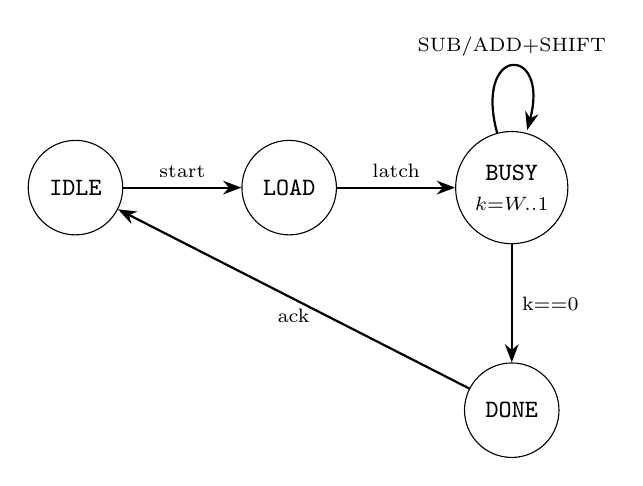
\begin{tikzpicture}[auto, node distance=15mm,
  state/.style={draw, circle, minimum size=12mm, align=center, font=\small\ttfamily},
  arr/.style={->, thick, >=Stealth}]
  \node[state] (idle) {IDLE};
  \node[state, right=of idle] (load) {LOAD};
  \node[state, right=of load] (busy) {BUSY\\{\scriptsize $k{=}W..1$}};
  \node[state, below=of busy] (done) {DONE};
  \draw[arr] (idle) -- node[above,font=\scriptsize]{start} (load);
  \draw[arr] (load) -- node[above,font=\scriptsize]{latch} (busy);
  \draw[arr] (busy) -- node[right,font=\scriptsize]{k==0} (done);
  \draw[arr] (busy) edge[loop above] node[font=\scriptsize]{SUB/ADD+SHIFT} (busy);
  \draw[arr] (done) -- node[below,font=\scriptsize]{ack} (idle);
\end{tikzpicture}
\caption{FSM divider non-restoring: IDLE$\to$LOAD$\to$BUSY ($W$ vòng)$\to$DONE. LPM\_DIVIDE ẩn FSM này trong IP, nhưng latency vẫn phải khớp twin.}
\label{fig:ch09_div_fsm}
\end{figure}

\paragraph{Cấu hình LPM\_DIVIDE.}
\begin{itemize}[leftmargin=1.4em]
\item Numerator: đủ chứa $f_s$ đã scale (vd 32-bit), hoặc $f_s\cdot 2^{f}$ nếu mang fractional $\tau$.
\item Denominator: $\tau_{\mathrm{fine}}$ fixed-point (vd Q16.16 sau parabolic).
\item Pipeline stages $=$ latency $L$ --- ghi vào comment RTL và twin.
\item Golden Mode~B: $f0_{\mathrm{Q12.4}} = (16000\cdot 16\cdot 65536 + (\tau_{\mathrm{fine,Q16}}\gg 1)) // \tau_{\mathrm{fine,Q16}}$ (chia có làm tròn).
\end{itemize}

\paragraph{RTL bọc (ý tưởng).}
\begin{verbatim}
// Sau tau_fine_q16 và fs=16000:
// start_div pulse -> chờ L chu kỳ -> f0_quot hợp lệ (Q12.4)
lpm_divide #(.LPM_WIDTHN(32), .LPM_WIDTHD(16), .LPM_PIPELINE(L))
  u_div (.clock(clk), .numer(fs_scaled), .denom(tau_q),
         .quotient(f0_quot));
\end{verbatim}

\subsection*{9.5. Twin Python bit-exact}

\begin{verbatim}
import numpy as np

def parabolic_delta(ym1, y0, yp1):
    denom = ym1 - 2.0 * y0 + yp1
    return 0.5 * (ym1 - yp1) / denom

def f0_q12_4(fs, tau_fine):
    return int(round(fs / float(tau_fine) * 16))

d = parabolic_delta(0.40, 0.50, 0.46)
assert abs(d - 3/14) < 1e-12
assert f0_q12_4(16000, 80 + d) == 3191
# TB: sau đúng L posedge, so quotient với twin
\end{verbatim}

Định dạng xuất giao tiếp (Chương~12): $F_0$ Q12.4 đóng gói \texttt{uint16} little-endian; $0$ = vô thanh; trần biểu diễn $4095{,}9375\,\text{Hz}$.

\subsection*{9.6. Chi phí silicon}

\begin{costbox}
\textbf{Ngân sách peak + parabolic + divider.}
\begin{itemize}[leftmargin=1.2em]
\item \textbf{Argmax} quét $\approx 187$ giá trị: vài ALM + comparator, 0 DSP, 0 M10K.
\item \textbf{Parabolic}: 2 trừ + 1 chia ngắn + nhân $1/2$ --- 0--1 DSP hoặc soft logic, vài chu kỳ.
\item \textbf{LPM\_DIVIDE} 32/16 pipeline: IP dùng ALM (và tùy chọn DSP); \emph{nút thắt là latency $L$}, không phải diện tích (chỉ 1 phép/khung).
\item \textbf{Non-restoring} tự viết $W$-bit: $\approx W$ chu kỳ, thuần ALM, dễ twin từng bước.
\item \textbf{M10K}: 0 cho khối này (trừ khi đệm kết quả nhiều khung).
\item Vì sao parabolic + 1 chia/khung: sai số $< 2\,\text{cent}$ điển hình (Chương~0); Sinc70/Sinc700 đắt hàng trăm phép nhân/đỉnh trong khi Viterbi đã tắt trên đường streaming.
\end{itemize}
\end{costbox}

\subsection*{9.7. Bài tập và lời giải giải thích}

\paragraph{Bài tập 9.1.} $r = [0{,}2,\ 0{,}6,\ 0{,}5]$ tại $\tau = 100,101,102$: tính $\Delta$, $\tau_{\mathrm{fine}}$, $F_0$ @ $16\,\text{kHz}$, mã Q12.4.

\paragraph{Bài tập 9.2.} Testbench: $16000/80 = 200$. Cố ý đọc quotient sớm 1 chu kỳ --- quan sát triệu chứng gắn nhầm khung.

\paragraph{Bài tập 9.3.} Với bộ $(0{,}40,0{,}50,0{,}46)$, so $\Delta$ parabolic với ý nghĩa ``đỉnh lệch phải''. Nếu mẫu số $r_{-}-2r^{*}+r_{+} > 0$, đó có còn là đỉnh không?

\noindent\textbf{Lời giải giải thích.}
\begin{enumerate}[leftmargin=1.4em]
\item Đỉnh nguyên tại $\tau^{*} = 101$ ($0{,}6$ lớn nhất). $\Delta = 0{,}5\cdot(0{,}2-0{,}5)/(0{,}2-1{,}2+0{,}5) = 0{,}5\cdot(-0{,}3)/(-0{,}5) = 0{,}3$. $\tau_{\mathrm{fine}} = 101{,}3$, $F_0 \approx 157{,}9467\,\text{Hz}$, Q12.4 $= 2527$.
\item Đọc sớm 1 ck lấy thương của lần chia trước (hoặc giá trị chưa ổn định). Triệu chứng điển hình: đường $F_0$ ``trễ một hop'' so với twin, cent error nhảy có hệ thống theo thời gian chứ không theo biên độ.
\item $\Delta = +3/14 > 0$: đỉnh thật hơi bên phải $\tau^{*}$. Nếu mẫu số $>0$ thì độ cong hướng lên --- đó là đáy (cực tiểu), không được lấy làm chu kỳ dây thanh; RTL phải kiểm tra mẫu số $<0$ hoặc dựa vào argmax đã chọn cực đại.
\end{enumerate}

\clearpage
\phantomsection
\section*{Chương 10. Silence / voicing / median-3 (Viterbi trên HPS)}
\addcontentsline{toc}{section}{Chương 10. Silence / voicing / median-3 (Viterbi trên HPS)}
\pdfbookmark[1]{Chương 10. Silence / voicing / median-3 (Viterbi trên HPS)}{chuong10}

\begin{learningobj}
Sau chương này bạn thiết kế cổng voicing/silence từ $r_a$ và năng lượng; triển khai median-3 (trễ 1 khung); giải thích vì sao Viterbi mặc định tắt trên fabric; tính tay ví dụ số; và đọc hộp chi phí.
\end{learningobj}

\begin{firstprin}{Vật lý: dây thanh không rung liên tục --- khi nào báo $F_0=0$?}
Hơi thở, khoảng lặng, phụ âm vô thanh cho $r_a$ thấp. Nếu vẫn báo $F_0$, đường pitch ``rung'' vô nghĩa. Praat gắn cờ voiced/unvoiced rồi (tuỳ chọn) chạy Viterbi/\texttt{pathFinder} theo chi phí octave và V$\leftrightarrow$UV. Trên Cyclone~V: \textbf{voicing gate + median-3 trên fabric} (rẻ, trễ đúng 1 hop); \textbf{Viterbi tắt trên fabric}, soft-float trên HPS khi cần đường cong ``Praat đầy đủ''.
\end{firstprin}

\subsection*{Toán --- voicing, silence, median-3, Viterbi}

\textbf{Voicing.} Sau chuẩn hóa $r_a[\tau^*]\in[0,1]$:
\[
\mathrm{voiced}=\bigl(r_a[\tau^*]\ge V\bigr)\;\land\;
\bigl(P_{\mathrm{local}}\ge S\cdot P_{\mathrm{global}}\bigr),
\]
với $V\approx0{,}45$ (voicingThreshold), $S$ = silenceThreshold (vd $0{,}03$). $P_{\mathrm{local}}=\max|x|$ trên khung; $P_{\mathrm{global}}$ = max chậm (IIR/max-hold) vì streaming không nhìn cả câu.

\textbf{Ứng viên Unvoiced strength} (Praat-like):
\[
s_{\mathrm{UV}}=V+\max\Bigl(0,\ 2-\frac{P_{\mathrm{local}}/P_{\mathrm{global}}}{S/(1+V)}\Bigr).
\]
Nếu $s_{\mathrm{UV}}$ thắng mọi đỉnh $\Rightarrow F_0=0$.

\textbf{Median-3.} Với ba giá trị liên tiếp $a,b,c$:
\[
\mathrm{med}=\max\bigl(\min(a,b),\ \min\bigl(\max(a,b),c\bigr)\bigr).
\]
RTL chốt median vào thanh ghi và xuất ở khung \emph{sau} --- trễ nhóm đúng 1 hop ($\approx10$\,ms).

\textbf{Viterbi (HPS).} $V(t,j)=\delta(t,j)+\max_i[V(t-1,i)-c_{ij}]$; $c_{ij}$ gồm jumpCost$\cdot|\log_2(f_j/f_i)|$ và vuvCost. Không hiện thực DP này trên fabric mặc định.

\subsection*{Ví dụ tính tay (đã kiểm Python)}

\paragraph{Median-3.} Chuỗi $200,\ 210,\ 80,\ 205,\ 208$:
cửa $(200,210,80)\to200$ (đập spike 80); $(210,80,205)\to205$; $(80,205,208)\to205$.

\paragraph{Voicing Q1.14.} $V=\mathrm{floor}(0{,}45\cdot2^{14})=7372$. Khung sine $r_a=12000$, $P_{\mathrm{loc}}=3277$, $P_{\mathrm{glob}}=30000$: voiced. Khung nhỏ $P_{\mathrm{loc}}=200$: silence chặn dù $r_a$ tạm ổn.

\paragraph{$s_{\mathrm{UV}}$.} $P_{\mathrm{local}}=0{,}02$, $P_{\mathrm{global}}=1$, $S=0{,}03$, $V=0{,}45$:
\[
s_{\mathrm{UV}}=0{,}45+\max\bigl(0,\ 2-\tfrac{0{,}02}{0{,}03/1{,}45}\bigr)\approx1{,}483.
\]

\paragraph{Viterbi $2\times2$.} $\delta=\begin{bmatrix}0{,}50&0{,}40\\0{,}45&0{,}48\end{bmatrix}$; cost V--V$=0{,}05$, V--UV$=0{,}14$. Cum $t2$ V: $\max(0{,}50-0{,}05,\ 0{,}40-0{,}14)+0{,}45=0{,}90$ $\Rightarrow$ đường V$\to$V.

\subsection*{RTL median-3 (ý tưởng)}

\begin{verbatim}
// Khi in_valid: tinh med = median(f1,f2,f3); chốt m_reg <= med;
// f_out <= m_reg chi khi in_valid ke (tre 1 khung)
\end{verbatim}

Không IP cho voicing/median --- thuần ALM. Viterbi: tiến trình HPS, shared memory / Avalon-MM.

\begin{costbox}
\textbf{Ngân sách silicon --- giải thích từng mục.}
\begin{itemize}[leftmargin=1.2em]
\item Voicing gate: vài so sánh --- $<50$ ALM, 0 DSP, 0 M10K.
\item Median-3: $<100$ ALM, trễ 1 hop, 0 DSP.
\item Max-hold $P_{\mathrm{global}}$: vài ALM.
\item Viterbi fabric: 0 (tắt). HPS soft nếu cần.
\item Vì sao median thay Viterbi: đập spike đơn đủ lab; DP $O(TK^2)$ cần đa ứng viên và BRAM path metric.
\end{itemize}
\end{costbox}

\subsection*{Thực hành}

\begin{enumerate}[leftmargin=1.4em]
\item Chuỗi $100,400,110$: median-3 cửa đầu ra gì? (100 --- đập 400 octave jump giả).
\item $s_{\mathrm{UV}}$ với $P_{\mathrm{local}}=P_{\mathrm{global}}$: chứng minh silence không kích.
\item Liệt kê 2 lý do không port pathFinder lên fabric ở lab này.
\end{enumerate}

\noindent\textbf{Mở rộng.} Ngưỡng voicing $r_a[\tau^*]\ge \theta$ (vd $\theta=0{,}45$ lab) quyết định voiced/unvoiced. Median-3 trên ba khung liên tiếp chống ``bật/tắt'' giả. Octave cost và VUV cost (Ch.~1) chỉ vào Viterbi pathFinder --- không sửa $r_a$ thô. Twin: dump cờ voiced + $F_0$ từng khung so Praat trên cùng wav.


\clearpage
\phantomsection
\section*{Chương 11. FSM tích hợp và Avalon-ST (valid/ready)}
\addcontentsline{toc}{section}{Chương 11. FSM tích hợp và Avalon-ST (valid/ready)}
\pdfbookmark[1]{Chương 11. FSM tích hợp và Avalon-ST (valid/ready)}{chuong11}

\begin{learningobj}
Sau chương này bạn giải thích được handshake Avalon-ST; vì sao source phải giữ data khi ready$=0$; đếm beat đúng khi có gap; nối FSM pitch (idle$\to$fill$\to$window$\to$mac$\to$peak$\to$pack); và đọc hộp chi phí adapter.
\end{learningobj}

\begin{firstprin}{Vì sao cần \texttt{valid}/\texttt{ready}? --- ống nước có van hai đầu}
\textbf{Avalon-ST} (Streaming) là quy ước Intel: mỗi nhịp đồng hồ, bên gửi (\emph{source}) khẳng định ``có data'' bằng \texttt{valid}; bên nhận (\emph{sink}) khẳng định ``tôi nhận được'' bằng \texttt{ready}. Một \textbf{beat} (một mẫu/từ thực sự chuyển) chỉ xảy ra khi \emph{cả hai} $=1$ trong cùng chu kỳ. Đây không phải hiện tượng âm thanh --- đây là hợp đồng silicon để hai khối khác tốc độ không làm mất hay nhân đôi mẫu. Mất một mẫu trong khung 640 $=$ lệch cửa sổ $=$ sai $\mathcal{R}_x$ $=$ sai $F_0$ im lặng.
\end{firstprin}

\subsection*{Quy ước từng tín hiệu}

\begin{itemize}[leftmargin=1.4em]
\item \texttt{valid}: source có data ổn định trên bus \emph{trong chu kỳ này}.
\item \texttt{ready}: sink sẽ chốt data nếu \texttt{valid}$=1$.
\item Beat: $\texttt{valid}\land\texttt{ready}$. Đếm beat trong TB phải khớp số mẫu gửi.
\item \textbf{Backpressure:} sink kéo \texttt{ready}$=0$ $\Rightarrow$ source \emph{giữ nguyên} data và \texttt{valid} (không nhảy mẫu tiếp).
\item \texttt{readyLatency}$=0$ (phổ biến): \texttt{ready} cùng chu kỳ với quyết định nhận. \texttt{readyLatency}$=1$: sink báo trước 1 ck --- đọc UG Avalon~683091 trước khi nối IP.
\end{itemize}

\subsection*{Ví dụ tính tay --- 6 chu kỳ có gap (đã kiểm logic)}

Nguồn muốn gửi 4 mẫu $\{A,B,C,D\}$. Giữa $B$ và $C$, sink kéo \texttt{ready}$=0$ đúng 2 ck; sau đó source tự kéo \texttt{valid}$=0$ đúng 1 ck (gap chủ động):

\begin{center}\small
\begin{tabular}{@{}cllll@{}}\toprule
ck & valid & ready & data & beat? \\
\midrule
1 & 1 & 1 & $A$ & có \\
2 & 1 & 1 & $B$ & có \\
3 & 1 & 0 & $B$ & không (giữ $B$) \\
4 & 1 & 0 & $B$ & không \\
5 & 1 & 1 & $B$? chờ --- thực ra sau ready lại: $C$ nếu đã advance & --- \\
\bottomrule
\end{tabular}
\end{center}

\noindent Làm đúng: sau ck2 đã chuyển $B$; ck3--4 source giữ $C$ (mẫu tiếp) với valid$=1$ ready$=0$; ck5 ready$=1$ $\Rightarrow$ beat $C$; rồi valid gap 1 ck; rồi beat $D$. Tổng beat $=4$. Đếm 3 hoặc 5 $\Rightarrow$ bug backpressure.

\begin{figure}[H]
\centering
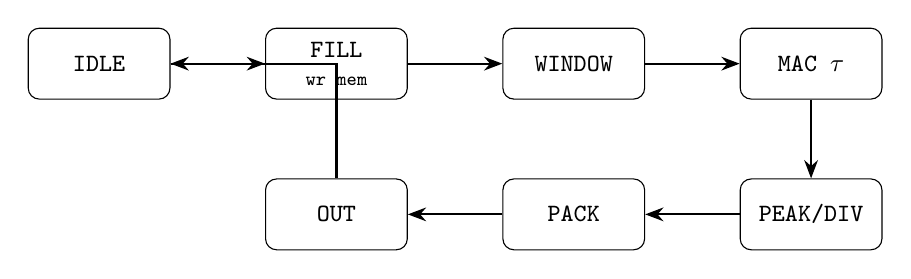
\begin{tikzpicture}[
  state/.style={draw, rounded corners, align=center, font=\small\ttfamily, minimum width=18mm, minimum height=9mm},
  arr/.style={->, thick, >=Stealth}]
  \node[state] (idle) {IDLE};
  \node[state, right=12mm of idle] (fill) {FILL\\[-1pt]{\scriptsize wr mem}};
  \node[state, right=12mm of fill] (win) {WINDOW};
  \node[state, right=12mm of win] (mac) {MAC $\tau$};
  \node[state, below=10mm of mac] (peak) {PEAK/DIV};
  \node[state, left=12mm of peak] (pack) {PACK};
  \node[state, left=12mm of pack] (out) {OUT};
  \draw[arr] (idle)--(fill); \draw[arr] (fill)--(win); \draw[arr] (win)--(mac);
  \draw[arr] (mac)--(peak); \draw[arr] (peak)--(pack); \draw[arr] (pack)--(out);
  \draw[arr] (out) |- (idle);
\end{tikzpicture}
\caption{FSM pitch rút gọn: FILL đủ $L$ mẫu $\to$ WINDOW $\to$ MAC mọi $\tau$ $\to$ PEAK/DIV $\to$ PACK Q12.4 $\to$ OUT (Avalon-ST). Mỗi mũi tên tôn trọng valid/ready với khối sau.}
\end{figure}

\subsection*{RTL --- giữ data khi backpressure}

\begin{verbatim}
// Source side: do NOT advance rd_ptr unless (valid && ready)
always @(posedge clk or negedge rst_n) begin
  if (!rst_n) begin out_valid <= 0; out_data <= 0; end
  else if (!out_valid || out_ready) begin
    // can load new beat
    if (have_sample) begin
      out_data  <= next_sample;
      out_valid <= 1'b1;
    end else out_valid <= 1'b0;
  end
  // else: hold out_data and out_valid (== backpressure)
end
\end{verbatim}

\subsection*{Twin đếm beat}

\begin{verbatim}
beats = 0
for cycle in sim_trace:
    if cycle["valid"] and cycle["ready"]:
        beats += 1
assert beats == n_samples_sent
\end{verbatim}

\begin{costbox}
\textbf{Ngân sách silicon --- giải thích từng mục.}
\begin{itemize}[leftmargin=1.2em]
\item Adapter valid/ready: $\sim0$--20 ALM; 0 DSP; 0 M10K.
\item FSM tích hợp: vài trăm ALM tùy số trạng thái và datapath mux.
\item Vì sao giữ data khi $\mathrm{ready}=0$: mất mẫu $=$ lệch khung $=$ sai $F_0$ không có warning synth.
\item readyLatency: phải khớp IP FIR/FFT nếu nối --- lệch 1 $=$ mất beat đầu/cuối burst.
\end{itemize}
\end{costbox}

\subsection*{Thực hành}

\begin{enumerate}[leftmargin=1.4em]
\item Vẽ waveform 8 ck: gửi 3 mẫu, ready$=0$ trong 3 ck giữa mẫu 1 và 2; đếm beat.
\item Sửa bug cố ý: advance ptr khi valid dù ready$=0$ --- TB đếm beat kỳ vọng fail thế nào?
\item Nối MAC$\to$peak: peak chậm hơn MAC; chứng minh source MAC giữ $\mathcal{R}_x[\tau]$ đúng.
\end{enumerate}

\noindent\textbf{Mở rộng.} Avalon-ST: nguồn chỉ đổi data khi \texttt{valid}\&\texttt{ready}; đích phải giữ data đã chấp nhận. Backpressure = \texttt{ready}=0 vài chu kỳ --- RTL không được mất mẫu. Twin đếm beat: số mẫu vào = số mẫu qua mỗi stage (trừ chỗ cố ý decimate). FSM pitch: IDLE$\to$FILL$\to$WINDOW$\to$MAC$\to$PEAK$\to$OUT.


\clearpage
\phantomsection
\section*{Chương 12. Đóng gói $F_0$ Q12.4 little-endian}
\addcontentsline{toc}{section}{Chương 12. Đóng gói F0 Q12.4}
\pdfbookmark[1]{Chương 12. Đóng gói F0 Q12.4}{chuong12}

\begin{learningobj}
Sau chương này bạn đóng $F_0$ thành uint16 Q12.4 LE; giải thích từng bit; xử lý UV$=0$ và bão hòa ceiling; viết twin \texttt{struct.pack}; và hiểu vì sao lỗi endian là lỗi giao thức chứ không phải lỗi pitch.
\end{learningobj}

\begin{firstprin}{Hợp đồng số: server đọc gì từ FPGA?}
Khối ước lượng trên FPGA không nói chuyện với server bằng số thực dấu phẩy động. Hợp đồng là một từ 16~bit không dấu theo thang \textbf{Q12.4}: 12 bit nguyên + 4 bit frac $\Rightarrow$ giá trị nguyên $=F_0^{\mathrm{Hz}}\times 16$. Ghi \textbf{little-endian} trên tệp \texttt{pitch\_f0.bin}: byte thấp trước. Khung vô thanh (\textbf{unvoiced}, UV) gửi đúng $0$ --- không NaN, không mã đặc biệt. Đảo endian hoặc quên chia 16 phía server làm $F_0$ lệch $\times256$ hoặc $\times16$ trong khi silicon vẫn đúng --- đó là lỗi \emph{giao thức}, không phải lỗi thuật toán.
\end{firstprin}

\subsection*{Toán --- từng ký hiệu}

Q12.4 nghĩa là 12 bit phần nguyên và 4 bit phần thập phân cố định: giá trị thực $=N/16$ Hz. Phạm vi không dấu $0..(2^{12}-2^{-4})$ Hz; có dấu thì thêm bit dấu tùy pack. Chọn 4 bit frac vì $\Delta=0{,}0625$\,Hz --- nhỏ hơn nhiều so với ngân sách vài chục cent ở 100--300\,Hz. Ký hiệu: $F_q=\mathrm{sat}(\mathrm{round}(F_0\cdot 16))$. Unpack: $\hat F=F_q/16$.

\subsection*{Ví dụ tính tay (đã kiểm Python)}

\begin{center}\small
\begin{tabular}{@{}llll@{}}\toprule
$F_0$ Hz & Q12.4 uint16 & bytes LE & ghi chú \\
\midrule
0 (UV) & 0 & \texttt{00 00} & \\
75{,}0 & 1200 & \texttt{B0 04} & floor \\
150{,}0625 & 2401 & \texttt{61 09} & \\
199{,}466 & 3191 & \texttt{77 0C} & parabolic Ch.~9 \\
200{,}0 & 3200 & \texttt{80 0C} & \\
440{,}0 & 7040 & \texttt{80 1B} & \\
600{,}0 & 9600 & \texttt{80 25} & ceil \\
700{,}0 & 9600 & \texttt{80 25} & sat ceil \\
\bottomrule
\end{tabular}
\end{center}

\subsection*{RTL pack}

\begin{verbatim}
module pack_q124 #(parameter CEIL_Q = 16'd9600)(
  input  wire clk, rst_n, in_valid, voiced,
  input  wire [15:0] f0_hz_u,   // Hz integer
  input  wire [3:0]  f0_frac,   // /16 bits if any
  output reg  out_valid,
  output reg  [15:0] q124,
  output reg  [7:0]  b0, b1
);
  wire [16:0] raw = {1'b0, f0_hz_u, 4'b0} + f0_frac;
  wire [15:0] sat = (raw > CEIL_Q) ? CEIL_Q : raw[15:0];
  always @(posedge clk or negedge rst_n)
    if (!rst_n) begin q124<=0; b0<=0; b1<=0; out_valid<=0; end
    else if (in_valid) begin
      q124 <= voiced ? sat : 16'd0;
      b0   <= voiced ? sat[7:0]  : 8'd0;
      b1   <= voiced ? sat[15:8] : 8'd0;
      out_valid <= 1'b1;
    end else out_valid <= 1'b0;
endmodule
\end{verbatim}

\subsection*{Twin bit-exact}

\begin{verbatim}
import numpy as np, struct
CEIL = 9600
def pack_q124(f0_hz, voiced=True):
    if not voiced or f0_hz <= 0: q = 0
    else: q = max(0, min(CEIL, int(np.round(f0_hz * 16.0))))
    return q, struct.pack("<H", q)
assert pack_q124(200.0)[1] == b"\x80\x0c"
assert pack_q124(199.466)[0] == 3191
assert pack_q124(0.0, False)[0] == 0
assert pack_q124(700.0)[0] == CEIL
\end{verbatim}

\begin{costbox}
\textbf{Ngân sách silicon --- giải thích từng mục.}
\begin{itemize}[leftmargin=1.2em]
\item Pack: vài ALM (dịch, sat, mux UV), 0 DSP, 0 M10K.
\item FIFO HPS (tuỳ chọn): 1 M10K cho burst khung.
\item Vì sao Q12.4: đủ 75--600\,Hz trong 16 bit; bước nhỏ hơn sai số ước lượng; LE khớp hầu hết CPU/HPS.
\item Vì sao UV$=0$: một giá trị đặc biệt duy nhất --- server không cần enum riêng.
\end{itemize}
\end{costbox}

\subsection*{Thực hành}

\begin{enumerate}[leftmargin=1.4em]
\item Pack 220\,Hz: kỳ vọng $3520=$ \texttt{C0 0D}.
\item Đổi big-endian cố ý: evaluator lệch bao nhiêu? (đọc nhầm $\times$ đến hàng trăm Hz).
\item UV phải \texttt{00 00}, không phải $0{,}01$\,Hz ($q=0$ vs $q=1$).
\end{enumerate}

\noindent\textbf{Mở rộng.} Q12.4 đóng gói $F_0$ Hz: 12 bit nguyên + 4 bit thập phân ($\Delta=1/16$\,Hz). Ví dụ $150{,}25$\,Hz $\to$ $150\cdot16+4=2404$. Tràn sat về max. Twin pack/unpack bit-exact với RTL; so lệch $<0{,}0625$\,Hz trước khi đổi sang cent.


\clearpage
\phantomsection
\section*{Chương 13. Kiểm chứng ba tầng: float / fixed / RTL}
\addcontentsline{toc}{section}{Chương 13. Kiểm chứng ba tầng: float / fixed / RTL}
\pdfbookmark[1]{Chương 13. Kiểm chứng ba tầng: float / fixed / RTL}{chuong13}

\begin{learningobj}
Sau Chương~13, người học sẽ:
\begin{enumerate}[leftmargin=1.4em]
    \item Vận hành được quy trình kiểm chứng ba tầng: (1)~mô hình float đối chiếu Praat; (2)~mô hình dấu phẩy tĩnh twin đối chiếu float; (3)~RTL/sim đối chiếu twin bit-exact.
    \item Định nghĩa và tính tay được ba chỉ số cổ điển \textbf{GPE}, \textbf{VDE}, \textbf{FFE} (Gross Pitch Error, Voicing Decision Error, Fine/F0 Frame Error) kèm ví dụ số đã kiểm Python.
    \item Viết testbench Avalon-ST có \texttt{valid}-gap và backpressure, đếm beat, so Q12.4 với golden.
    \item Điền bảng tài nguyên từ báo cáo Fitter thật (không bịa số), và giải thích vì sao mỗi tầng bắt một lớp lỗi khác nhau.
\end{enumerate}
\end{learningobj}

\subsection*{13.1. Hiện tượng thật: ba tầng bắt ba lớp lỗi}

\begin{firstprin}{Silicon không chạy Python --- hãy khoanh đúng lớp}
Một đường $F_0$ sai có thể đến từ rất nhiều chỗ: nhầm công thức Boersma, sai Q-format, sai handshake, quên bão hòa, đảo endian. Nếu nhảy thẳng vào Signal Tap trên DE10, bạn sẽ mất ngày để đoán. Ba tầng kiểm chứng tách bạch ba lớp:
\begin{itemize}[leftmargin=1.4em]
    \item \textbf{Tầng 1 --- Float vs Praat:} cùng wav, cùng time step $10\,\text{ms}$, cùng floor/ceiling $75$--$600\,\text{Hz}$. Sai ở đây là sai \emph{thuật toán / thứ tự bước} (quên chuẩn hóa $C[\tau]$, sai parabolic, tắt nhầm silence gate).
    \item \textbf{Tầng 2 --- Fixed twin vs Float:} cùng công thức nhưng mọi phép toán dùng Q$m.n$, round/sat/shift giống RTL. Sai ở đây là sai \emph{lượng tử hóa và làm tròn}.
    \item \textbf{Tầng 3 --- RTL vs Fixed:} ModelSim/Questa hoặc Signal Tap dump từng mẫu/từng khung. Mục tiêu lab: \textbf{$0$ bit mismatch} trên vector golden. Sai ở đây là sai \emph{handshake, latency, reset, X-propagation}.
\end{itemize}
Nhảy thẳng tầng~3 khi tầng~1 còn đỏ chính là lãng phí ngày debug FSM.
\end{firstprin}

Ba vector bắt buộc mọi khối tiền xử lý (đã nêu Chương~3): \texttt{zero} (toàn $0$), \texttt{DC} (hằng khác $0$), \texttt{clip} (đụng $\pm 32767$). Thêm vector sine $75/100/200/440/590\,\text{Hz}$, nhiễu trắng, âm xát $/s/$, và hai đoạn giọng thật --- cùng tinh thần \texttt{verify\_tiers.py}.

\begin{figure}[H]
\centering
\begin{tikzpicture}[font=\small, >=Stealth,
  tier/.style={draw, rounded corners, align=center, minimum width=3.6cm, minimum height=1.15cm}]
  \node[tier, fill=blue!10] (t1) {Tầng 1\\Float $\leftrightarrow$ Praat\\GPE / VDE / FFE};
  \node[tier, fill=teal!10, right=1.1cm of t1] (t2) {Tầng 2\\Fixed $\leftrightarrow$ Float\\sai số cent / Q};
  \node[tier, fill=orange!12, right=1.1cm of t2] (t3) {Tầng 3\\RTL $\leftrightarrow$ Fixed\\bit-exact + beat};
  \draw[->, very thick] (t1)-- (t2);
  \draw[->, very thick] (t2)-- (t3);
  \node[below=0.45cm of t1, font=\scriptsize, align=center]{Công thức\\thứ tự bước};
  \node[below=0.45cm of t2, font=\scriptsize, align=center]{Q-format\\round / sat};
  \node[below=0.45cm of t3, font=\scriptsize, align=center]{Handshake\\latency / X};
\end{tikzpicture}
\caption{Ba tầng kiểm chứng: mỗi tầng khoanh một lớp lỗi; chỉ xuống tầng dưới khi tầng trên đã xanh trên cùng bộ vector.}
\label{fig:ch13_three_tiers}
\end{figure}

\subsection*{13.2. Toán: GPE, VDE, FFE --- định nghĩa từng ký hiệu}

Trong đánh giá cao độ chuẩn (Rabiner, Chu \& Alwan, v.v.), mỗi khung được gắn nhãn hữu thanh/vô thanh bởi tham chiếu (ở đây: Praat) và bởi hệ thống (float / fixed / RTL). Ký hiệu:
\begin{itemize}[leftmargin=1.4em]
    \item $N$: tổng số khung có mặt cả hai hệ thống.
    \item $N_{VV}$: số khung cả tham chiếu lẫn hệ thống đều hữu thanh.
    \item $F_{\mathrm{ref}}[k]$, $F_{\mathrm{hw}}[k]$: cao độ (Hz) trên các khung cùng hữu thanh.
\end{itemize}

\paragraph{GPE --- Gross Pitch Error (Sai cao độ thô).}
\begin{equation}
\label{eq:ch13_gpe}
\mathrm{GPE}=\frac{1}{N_{VV}}\bigl|\bigl\{k\in VV:\ \bigl|F_{\mathrm{hw}}[k]/F_{\mathrm{ref}}[k]-1\bigr|>0{,}2\bigr\}\bigr|.
\end{equation}
Ngưỡng $20\%$ roughly một quãng gần (khoảng lớn hơn sai số tinh). GPE cao thường báo octave error ($F_0/2$ hoặc $2F_0$) --- đúng bệnh Chương~8--10 khi quên $C[\tau]$ hoặc voicing nuốt đỉnh đúng.

\paragraph{VDE --- Voicing Decision Error (Sai quyết định hữu/vô thanh).}
\begin{equation}
\label{eq:ch13_vde}
\mathrm{VDE}=\frac{N_{\mathrm{FV}}+N_{\mathrm{FU}}}{N},
\end{equation}
với $N_{\mathrm{FV}}$ = false voiced (hệ thống báo V khi tham chiếu UV), $N_{\mathrm{FU}}$ = false unvoiced (ngược lại). VDE cao $\Rightarrow$ xem lại ngưỡng $V$, $S$, warmup $P_{\mathrm{global}}$ (Chương~10).

\paragraph{FFE --- F0 Frame Error (gộp).}
Nhiều báo cáo lab định nghĩa FFE là tỷ lệ khung ``hỏng'' theo nghĩa \emph{hoặc} sai voicing \emph{hoặc} GPE trên khung cùng hữu thanh:
\begin{equation}
\label{eq:ch13_ffe}
\mathrm{FFE}=\frac{N_{\mathrm{VDE\ frames}}+N_{\mathrm{GPE\ frames}}}{N}.
\end{equation}
(Một số tài liệu gọi ``Fine Error'' là sai số cent trung bình trên khung \emph{không} GPE; lab này dùng FFE dạng frame-error tổng hợp như trên và ghi rõ trong báo cáo.)

\paragraph{Sai số cent trên khung ``tinh''.}
\begin{equation}
\Delta_{\mathrm{cent}}[k]=1200\log_2\bigl(F_{\mathrm{hw}}[k]/F_{\mathrm{ref}}[k]\bigr).
\end{equation}
Ngân sách lab trên sine/giọng sạch: $\max|\Delta_{\mathrm{cent}}| < 20$---$30$~cent sau khi đã loại khung GPE (nếu có). Mỗi stage (DC, FIR lượng tử, window Q1.15, MAC cắt bit, $C[\tau]$ Q3.13, parabolic, LPM\_DIVIDE, Q12.4) góp vài cent; vượt ngân sách thì lần ngược từ peak về FIR, không đoán.

\subsection*{13.3. Ví dụ tính tay --- chỉ số và cent (đã kiểm Python)}

\paragraph{Cent.} $F_{\mathrm{hw}}=199{,}466\,\text{Hz}$ (parabolic Chương~9), $F_{\mathrm{ref}}=200\,\text{Hz}$:
\[
\Delta_{\mathrm{cent}}=1200\log_2(199{,}466/200)\approx -4{,}629\,\text{cent}.
\]
Nằm trong ngân sách $20$~cent.

\paragraph{Đồ thị nhầm lẫn giả định $N=20$ khung.} Giả sử $N_{VV}=14$, trong đó $2$ khung lệch $>20\%$ (octave); thêm $3$ khung sai voicing (không trùng hai khung GPE):
\[
\mathrm{GPE}=\frac{2}{14}\approx 0{,}1429,\qquad
\mathrm{VDE}=\frac{3}{20}=0{,}15,\qquad
\mathrm{FFE}=\frac{5}{20}=0{,}25.
\]
Script \texttt{verify/verify\_chuong\_10\_14.py} khẳng định các tỷ số này. Trên sine sạch lab, mục tiêu thực tế: $\mathrm{GPE}\approx 0$, $\mathrm{VDE}$ thấp, $|\Delta_{\mathrm{cent}}|<20$.

\paragraph{LSB Q12.4.} Tại $200\,\text{Hz}$, $0{,}0625\,\text{Hz}$ $\approx 0{,}541\,\text{cent}$ --- nhỏ hơn nhiều so với $-4{,}6\,\text{cent}$ của parabolic ở ví dụ trên, nên tầng pack hiếm khi là thủ phạm GPE.


\paragraph{Ví dụ tính tay --- ma trận nhầm lẫn năm khung.}
Cho tham chiếu Praat và hệ thống (Hz; $0$ = UV):
\begin{center}\small
\begin{tabular}{@{}cccccc@{}}\toprule
$k$ & 0 & 1 & 2 & 3 & 4 \\
\midrule
$F_{\mathrm{ref}}$ & $200$ & $200$ & $0$ & $180$ & $0$ \\
$F_{\mathrm{hw}}$ & $199{,}5$ & $100$ & $0$ & $0$ & $50$ \\
Nhãn lỗi & tinh & GPE octave & OK UV & false UV & false V \\
\bottomrule
\end{tabular}
\end{center}
Khung cùng hữu thanh $VV=\{0,1\}$ ($N_{VV}=2$). Khung~$1$ có $|100/200-1|=0{,}5>0{,}2$ $\Rightarrow N_{\mathrm{GPE}}=1$. Sai voicing ở $k=3$ (FU) và $k=4$ (FV) $\Rightarrow N_{\mathrm{VDE}}=2$.
\[
\mathrm{GPE}=\frac{1}{2}=0{,}5,\qquad
\mathrm{VDE}=\frac{2}{5}=0{,}4,\qquad
\mathrm{FFE}=\frac{1+2}{5}=0{,}6.
\]
Script verify khẳng định $N_{\mathrm{GPE}}=1$, $N_{\mathrm{VDE}}=2$ trên đúng vector này.

\begin{figure}[H]
\centering
\begin{tikzpicture}[font=\small]
  \node[draw, fill=green!15, minimum width=2.2cm, minimum height=1.2cm, align=center] at (0,1.3) {TV\\đúng V};
  \node[draw, fill=red!15, minimum width=2.2cm, minimum height=1.2cm, align=center] at (2.6,1.3) {FV\\false V};
  \node[draw, fill=red!15, minimum width=2.2cm, minimum height=1.2cm, align=center] at (0,0) {FU\\false UV};
  \node[draw, fill=green!15, minimum width=2.2cm, minimum height=1.2cm, align=center] at (2.6,0) {TU\\đúng UV};
  \node[rotate=90, left] at (-1.5,0.65) {Tham chiếu};
  \node[above] at (1.3,2.1) {Hệ thống $\to$};
  \node[font=\scriptsize, align=left] at (6.2,0.65)
    {VDE $=(N_{\mathrm{FV}}+N_{\mathrm{FU}})/N$.\\
     GPE chỉ đếm trong ô TV\\khi $|F_{hw}/F_{ref}-1|>0{,}2$.};
\end{tikzpicture}
\caption{Hình 13.4 --- Ma trận hữu/vô thanh: VDE lấy hai ô đỏ; GPE lấy tập con của ô TV.}
\label{fig:ch13_confusion}
\end{figure}

\begin{figure}[H]
\centering
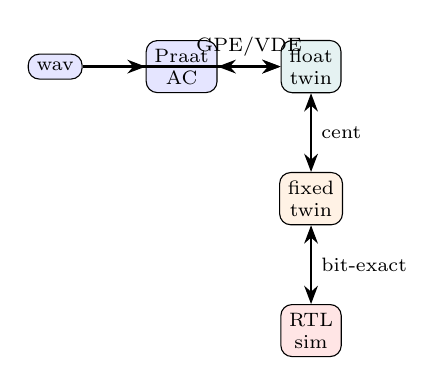
\begin{tikzpicture}[font=\scriptsize, >=Stealth,
  s/.style={draw, rounded corners, align=center, inner sep=3pt}]
  \node[s, fill=blue!10] (wav) {wav};
  \node[s, fill=blue!10, right=8mm of wav] (praat) {Praat\\AC};
  \node[s, fill=teal!10, right=8mm of praat] (flt) {float\\twin};
  \node[s, fill=orange!10, below=10mm of flt] (fix) {fixed\\twin};
  \node[s, fill=red!10, below=10mm of fix] (rtl) {RTL\\sim};
  \draw[->, thick] (wav)--(praat);
  \draw[->, thick] (wav)--(flt);
  \draw[<->, thick] (praat)--node[above]{GPE/VDE} (flt);
  \draw[<->, thick] (flt)--node[right]{cent} (fix);
  \draw[<->, thick] (fix)--node[right]{bit-exact} (rtl);
\end{tikzpicture}
\caption{Hình 13.5 --- Luồng đối sánh tầng 1$\to$2$\to$3 trên cùng wav.}
\label{fig:ch13_flow}
\end{figure}

\begin{figure}[H]
\centering
\begin{tikzpicture}[font=\scriptsize, x=0.7cm, y=0.45cm]
  \foreach \y/\lab in {6/valid, 4.5/ready, 3/data, 1.5/score} {
    \node[left] at (0,\y) {\lab};
  }
  \draw[very thick, blue] (1,5.7)--(1,6.3)--(3,6.3)--(3,5.7)--(4,5.7)--(4,6.3)--(10,6.3);
  \draw[very thick, teal] (1,4.2)--(1,4.8)--(5,4.8)--(5,4.2)--(7,4.2)--(7,4.8)--(10,4.8);
  \node at (2,3) {s0};
  \node at (4.5,3) {s1 giữ};
  \node at (8,3) {s1..};
  \fill[orange] (2,1.5) circle (2pt);
  \fill[orange] (8,1.5) circle (2pt);
  \node[font=\scriptsize, align=center] at (5.5,0.2)
    {TB phải hạ ready ngẫu nhiên; scoreboard chỉ chốt khi beat=1.};
\end{tikzpicture}
\caption{Hình 13.6 --- Testbench Avalon-ST: valid-gap + backpressure; chỉ chấm cam được so golden.}
\label{fig:ch13_tb_wave}
\end{figure}

\begin{figure}[H]
\centering
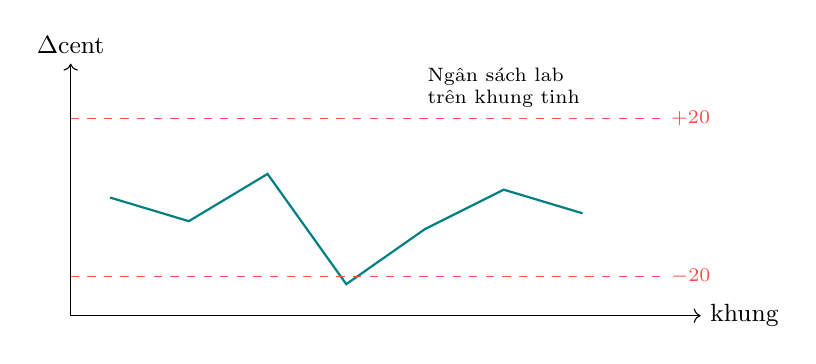
\begin{tikzpicture}[font=\small]
  \draw[->] (0,0)--(8,0) node[right]{khung};
  \draw[->] (0,0)--(0,3.2) node[above]{$\Delta$cent};
  \draw[thick, teal] (0.5,1.5)--(1.5,1.2)--(2.5,1.8)--(3.5,0.4)--(4.5,1.1)--(5.5,1.6)--(6.5,1.3);
  \draw[dashed, red!70] (0,2.5)--(7.5,2.5) node[right,font=\scriptsize]{$+20$};
  \draw[dashed, red!70] (0,0.5)--(7.5,0.5) node[right,font=\scriptsize]{$-20$};
  \node[font=\scriptsize, align=left] at (5.5,2.9){Ngân sách lab\\trên khung tinh};
\end{tikzpicture}
\caption{Hình 13.7 --- Sai số cent khung-tinh phải nằm trong $\pm 20$---$30$~cent sau khi loại GPE.}
\label{fig:ch13_cent_budget}
\end{figure}

\begin{figure}[H]
\centering
\begin{tikzpicture}[font=\scriptsize, >=Stealth,
  b/.style={draw, rounded corners, align=center, minimum width=2.4cm, minimum height=0.85cm}]
  \node[b, fill=red!12] (sym) {Symptom\\GPE cao};
  \node[b, fill=orange!12, right=10mm of sym] (t1) {Tầng 1?\\công thức};
  \node[b, fill=orange!12, right=10mm of t1] (t2) {Tầng 2?\\Q-format};
  \node[b, fill=orange!12, right=10mm of t2] (t3) {Tầng 3?\\handshake};
  \draw[->, thick] (sym)--(t1);
  \draw[->, thick] (t1)--(t2);
  \draw[->, thick] (t2)--(t3);
  \node[below=3mm of t1, align=center]{quên $C[\tau]$\\sai parabolic};
  \node[below=3mm of t2, align=center]{cắt MAC\\ROM endian};
  \node[below=3mm of t3, align=center]{mất beat\\đảo LE};
\end{tikzpicture}
\caption{Hình 13.8 --- Cây chẩn đoán: luôn hỏi tầng trên trước khi đụng Signal Tap.}
\label{fig:ch13_diag_tree}
\end{figure}


\subsection*{13.4. Tầng 1: Float vs Praat}

Thực hành khuyến nghị (Parselmouth hoặc Praat batch):
\begin{verbatim}
snd = parselmouth.Sound(wav, sampling_frequency=16000)
pm = snd.to_pitch_ac(time_step=0.01, pitch_floor=75, pitch_ceiling=600)
f_ref = pm.selected_array["frequency"]  # 0 = UV
# f_float: twin float_pitch_frame tung hop
# Do GPE/VDE/FFE chi tren khung overlap thoi gian
\end{verbatim}
Tham số bắt buộc khớp lab: time step $0{,}01\,\text{s}$, floor $75$, ceiling $600$, và (nếu đối chiếu sâu) cùng voicingThreshold $0{,}45$. Khác tham số $\Rightarrow$ ``sai số'' giả tạo.

\subsection*{13.4b. Tầng 1 sâu: khớp tham số Praat}

Ngoài time step / floor / ceiling, các tham số hay làm lệch giả tạo:
\begin{itemize}[leftmargin=1.4em]
  \item \texttt{voicingThreshold} (mặc định $0{,}45$): khác số $\Rightarrow$ VDE giả.
  \item \texttt{octaveCost} / \texttt{octaveJumpCost}: twin float lab tắt pathFinder thì không so được đường cong ``có Viterbi'' của Praat GUI mặc định --- phải gọi API/\texttt{Pitch.cpp} với cùng cờ tắt, hoặc chấp nhận so trên khung đã voiced ổn định.
  \item Đồng bộ thời gian: tâm cửa sổ lab tại $kH+L/2$; Praat time step $0{,}01\,\text{s}$ phải neo cùng gốc.
\end{itemize}

\paragraph{Ví dụ tính tay --- RTF mô phỏng $1\,\text{s}$.}
Số khung $97$, mỗi khung $\approx 120\,960$ chu kỳ MAC:
\[
T_{\mathrm{proc}}=\frac{120\,960\cdot 97}{50\cdot 10^6}\approx 0{,}2347\,\text{s},
\qquad \mathrm{RTF}\approx 0{,}2347
\]
(RTF = \emph{Real-Time Factor} = thời gian xử lý / thời gian âm thanh; đã kiểm script). Một TB chu kỳ-chính xác cho $1\,\text{s}$ audio vì thế chạy khoảng $0{,}23\,\text{s}$ thời gian mô phỏng xung nhịp (wall-clock phụ thuộc tốc độ sim).

\subsection*{13.5. Tầng 2: Fixed twin vs Float}

Twin cố định bit dùng cùng ROM Hanning Q1.15, ROM $C[\tau]$ Q3.13, cùng sat/shift như RTL. Đo:
\begin{itemize}[leftmargin=1.4em]
    \item Sai lệch cent trung bình / max giữa $F_{\mathrm{fixed}}$ và $F_{\mathrm{float}}$ trên khung cùng voiced;
    \item Số khung đổi voicing so với float (thường $0$ trên sine).
\end{itemize}
Nếu tầng~1 xanh mà tầng~2 đỏ: nghi ngờ cắt bit MAC, quên dịch BFP (\emph{Block Floating Point} --- mỗi khối FFT chia sẻ một exponent; nếu dùng FFT IP), hoặc ROM $C[\tau]$ sai endian trong hex.

\subsection*{13.5b. Tầng 2 sâu: nguồn cent cố định bit}

Mỗi khối góp sai số lượng tử xấp xỉ (thứ tự độ lớn, không phải định lý):
\begin{itemize}[leftmargin=1.4em]
  \item Window Q1.15: hệ số mép khung lệch $1$ LSB $\to$ vài cent.
  \item MAC cắt về thanh ghi trung gian: nếu cắt quá sớm trước khi nhân $C[\tau]$, đỉnh $\tau$ lớn bị thiên vị.
  \item ROM $C[\tau]$ Q3.13: sai endian hex $\to$ GPE hàng loạt (lớp này đôi khi lộ sớm ở tầng~1 nếu float cũng đọc nhầm hex --- tách test ROM).
  \item LPM\_DIVIDE làm tròn quotient: thường $<1\,\text{cent}$ tại $200\,\text{Hz}$.
  \item Pack Q12.4: LSB $\approx 0{,}54\,\text{cent}$ tại $200\,\text{Hz}$.
\end{itemize}
Tổng ngân sách $20$--$30\,\text{cent}$ là ``hộp'' chứa cho cả chuỗi; vượt hộp thì lần từ pack ngược về FIR, đo cent từng điểm neo (sau window, sau MAC, sau $C[\tau]$, sau DIV).

\subsection*{13.6. Tầng 3: RTL vs Fixed --- bit-exact và testbench}

\paragraph{Hợp đồng bit-exact.} Trên cùng \texttt{golden\_pcm.hex}, mọi khung Q12.4 dump từ sim phải bằng twin fixed: $0$ bit lệch. Không ``gần đúng'' ở tầng này.

\paragraph{Testbench Avalon-ST.}
\begin{itemize}[leftmargin=1.4em]
    \item Đọc PCM hex $\to$ stream sample với \texttt{valid} có gap ngẫu nhiên (LFSR).
    \item Sink hạ \texttt{ready} ngẫu nhiên ở mọi stage (đặc biệt MAC$\leftrightarrow$peak, pack$\leftrightarrow$HPS).
    \item Đếm beat vào $=$ đếm beat ra (trừ decimate cố ý).
    \item Scoreboard so $F_q$ với \texttt{golden\_f0.hex}.
    \item Vector cạnh: zero / DC / clip phải cho $F_q=0$ hoặc hành vi DC-blocker đã định nghĩa (Chương~3).
\end{itemize}

\begin{verbatim}
delta_cent = 1200 * np.log2(f_hw / f_praat)
assert np.nanmax(np.abs(delta_cent[voiced_both])) < 20.0
assert (q_rtl == q_fixed).all()  # tang 3
\end{verbatim}

\paragraph{Tài liệu Intel cần mở đúng số.} Avalon~683091, FIR~683208, FFT~683374 (nếu bật), LPM\_DIVIDE handbook. Fmax/ALM/DSP/M10K lấy từ \emph{Fitter report} sau Place \& Route --- không bịa.

\subsection*{13.6b. Tầng 3 sâu: X-propagation và reset}

RTL sim phải:
\begin{enumerate}[leftmargin=1.4em]
  \item Khởi động \texttt{rst\_n}$=0$ đủ vài chu kỳ; mọi thanh ghi median/FSM về $0$.
  \item Không để \texttt{X} (trạng thái chưa xác định trong mô phỏng RTL --- bit chưa được gán $0/1$ sau reset) trên \texttt{valid}/\texttt{ready}: một \texttt{X} làm scoreboard ``xanh giả'' hoặc đỏ ngẫu nhiên.
  \item Dump $F_q$ chỉ khi beat OUT; so với \texttt{golden\_f0.hex} từ twin fixed cùng seed LFSR cho ready.
  \item Vector cạnh zero/DC/clip: kỳ vọng $F_q=0$ (hoặc hành vi DC-blocker đã khóa Chương~3).
\end{enumerate}

\subsection*{13.6c. Golden hex và tái lập bit-exact}

Mỗi revision RTL phải kèm:
\begin{itemize}[leftmargin=1.4em]
  \item \texttt{golden\_pcm.hex} --- vector vào (hoặc WAV gốc + script gen).
  \item \texttt{golden\_f0.hex} --- chuỗi $F_q$ từ twin fixed cùng tham số.
  \item Seed LFSR cho valid-gap/ready trong TB (ghi vào header test).
\end{itemize}
Không tái lập được seed thì ``bit-exact hôm qua'' không chứng minh được hôm nay. Khi đổi $V$, $S$, hoặc ROM $C[\tau]$, phải regenerate golden và ghi chú DIFF.

\paragraph{Ví dụ tính tay --- ngưỡng GPE $20\%$.}
Tại $F_{\mathrm{ref}}=200\,\text{Hz}$, biên GPE là $160$ và $240\,\text{Hz}$. Mọi ước lượng trong $(160,240)$ trên khung VV \emph{không} tính GPE (chỉ đóng góp cent tinh). Octave đúng $100$ hoặc $400$ nằm ngoài biên --- GPE chắc chắn. Đó là lý do GPE cao thường chỉ thẳng ROM $C[\tau]$ hoặc voicing nuốt đỉnh đúng rồi bám hài.

\paragraph{FFE và báo cáo.} Khi viết báo cáo lab, luôn định nghĩa FFE một lần (công thức~\eqref{eq:ch13_ffe}) và không trộn với ``fine error trung bình cent''. Người chấm cần biết bạn đang đếm \emph{tỷ lệ khung hỏng} chứ không phải trung bình cent.

\begin{physicalinsight}
Ba tầng không phải nghi thức nộp bài. Chúng là cách khoanh vùng nhanh: công thức, lượng tử, hay dây nối. Một TB ``end-to-end đỏ'' không nói bạn sửa chỗ nào; ba đèn xanh/đỏ nói được.
\end{physicalinsight}

\subsection*{13.7. Bảng tài nguyên (điền từ Fitter)}

\begin{center}\small
\begin{tabular}{@{}lcccc@{}}\toprule
Khối & ALM & DSP & M10K & Latency (ck) \\
\midrule
PLL + I\textsuperscript{2}S &  &  &  & \\
DC-blocker &  &  &  & \\
FIR $2/3$ &  &  &  & \\
Sliding RAM &  &  &  & \\
Window &  &  &  & \\
MAC ACF &  &  &  & \\
ROM $C[\tau]$ &  &  &  & \\
Peak + DIV &  &  &  & \\
Voicing + median-3 &  &  &  & \\
FSM + pack Q12.4 &  &  &  & \\
\midrule
\textbf{Tổng} (mục tiêu $\lesssim 850$ ALM, $3$ DSP, $4$ M10K) &  &  &  & \\
\bottomrule
\end{tabular}
\end{center}

\noindent Khi nộp bài (Chương~14), không được để trống các ô tổng nếu đã chạy Fitter --- điền số thật kèm ảnh chụp report.

\begin{costbox}
\textbf{Ngân sách xác minh --- giải thích từng mục.}
\begin{itemize}[leftmargin=1.2em]
    \item \textbf{Thời gian sim:} vài giây đến vài phút cho $1\,\text{s}$ audio @ $50\,\text{MHz}$ TB (tuỳ độ chi tiết dump).
    \item \textbf{Disk:} golden hex vài MB --- commit cùng revision RTL để tái lập.
    \item \textbf{Người:} không bỏ tầng float; mỗi fail gắn đúng tầng (GPE $\to$ thuật toán; cent fixed $\to$ Q-format; bit mismatch $\to$ RTL).
    \item \textbf{Vì sao ba tầng:} một TB ``tất cả'' không chỉ ra \emph{loại} lỗi; tách tầng rút ngắn chu kỳ sửa.
\end{itemize}
\end{costbox}


\subsection*{13.7b. Cách điền Fitter thật}

Sau Place \& Route trên Quartus Standard/Lite cho part \texttt{5CSXFC6D6F31C6N}:
\begin{enumerate}[leftmargin=1.4em]
  \item Mở \emph{Fitter $\to$ Resource Usage Summary}: copy ALM logic, DSP blocks, M10K.
  \item Mở \emph{Timing Analyzer}: Fmax của clock $50\,\text{MHz}$ (hoặc clock datapath thật).
  \item Breakdown theo hierarchy nếu tool cho phép --- tách MAC, FIR, FSM.
  \item Không lấy số từ Synthesis sớm (trước Fitter) làm số nộp: synthesis ước tính, Fitter mới là silicon mapping.
\end{enumerate}
Mục tiêu Chương~0: $\lesssim 850$ ALM, $3$ DSP, $4$ M10K, RTF $\approx 0{,}24$. Vượt M10K thường do FIFO/RAM thừa; vượt DSP do nhân cửa sổ + MAC + FIR không chia sẻ --- xét time-multiplex trước khi xin thêm.


\subsection*{13.7c. Liên hệ RTF, sim wall-time và Signal Tap}

RTF $\approx 0{,}23$ trên $1\,\text{s}$ audio nghĩa là mô phỏng chu kỳ-chính xác ``bắt kịp'' nhanh hơn realtime trên giấy; nhưng ModelSim/Questa có thể chậm hơn realtime tường vì diễn dịch. Đừng nhầm wall-time sim với RTF silicon. Signal Tap trên board đo realtime thật: nếu FIFO đầy liên tục, backpressure đang ăn biên $377\,000$ chu kỳ --- cần giảm dump hoặc tăng FIFO, không thêm DSP.

\paragraph{Ví dụ tính tay --- đếm khung overlap thời gian.} Praat và twin phải so trên cùng tập thời điểm. Nếu Praat trả $100$ khung và twin $97$ khung cho $1\,\text{s}$ (do neo cửa khác), chỉ lấy giao khoảng thời gian chung, ví dụ $90$ khung giữa. Tính GPE/VDE trên $N=90$ đó; không pad $0$ giả vào đuôi. Sai bước này tạo VDE giả ở biên câu.

\paragraph{Chuẩn bị báo cáo.} Mỗi tầng một mục: lệnh chạy, tham số, bảng chỉ số, kết luận xanh/đỏ. Đính kèm hash git của RTL + twin + golden. Người chấm tái lập được thì điểm phương pháp mới vững.

\paragraph{Trước khi sang Chương~14.} Tầng~1 cần GPE$\approx 0$ trên sine sạch; tầng~2 max cent $<20$; tầng~3 không lệch bit và đếm beat khớp. Ngoài zero/DC/clip/sine, giữ một đoạn xát vô thanh (ví dụ $/s/$) và một đoạn giọng có thanh điệu --- tránh VDE ``xanh giả'' vì toàn hữu thanh, và để Pearson có nghĩa.


\subsection*{13.8. Bài tập và lời giải giải thích}

\paragraph{Bài tập 13.1.} Chạy twin DC-blocker trên zero / DC / clip. Kỳ vọng đầu ra định tính?

\paragraph{Lời giải.} Zero $\to$ zero. DC hằng $\to$ sau vài hằng số thời gian $\alpha$, đầu ra $\to 0$ (zero tại $z=1$). Clip $\pm 32767$ xen kẽ $\to$ không được wrap thành âm lớn; sat\_16 giữ biên. Nếu clip tạo dao động limit-cycle, nghi \texttt{y\_acc} quá hẹp (Chương~3).

\paragraph{Bài tập 13.2.} Cố ý đảo endian Q12.4 trên golden $200\,\text{Hz}$. GPE/cent thay đổi thế nào?

\paragraph{Lời giải.} Server đọc $2048{,}75\,\text{Hz}$ (Chương~12). $|2048{,}75/200-1|\gg 0{,}2$ $\Rightarrow$ mọi khung đó thành GPE; $\Delta_{\mathrm{cent}}$ khổng lồ. Tầng~1 ``đỏ'' dù thuật toán đúng --- phải bắt bằng test pack/unpack trước khi đổ tội MAC.

\paragraph{Bài tập 13.3.} Cho $N=20$, $N_{VV}=14$, $2$ GPE, $3$ VDE (rời nhau). Tính GPE, VDE, FFE.

\paragraph{Lời giải.} $\mathrm{GPE}=2/14\approx 0{,}1429$, $\mathrm{VDE}=3/20=0{,}15$, $\mathrm{FFE}=5/20=0{,}25$ --- khớp script verify.

\clearpage
\phantomsection
\section*{Chương 14. Checklist nộp bài (một lần duy nhất)}
\addcontentsline{toc}{section}{Chương 14. Checklist nộp bài (một lần duy nhất)}
\pdfbookmark[1]{Chương 14. Checklist nộp bài (một lần duy nhất)}{chuong14}

\begin{learningobj}
Trước khi nộp bài hoặc đóng gói bitfile, bạn đọc từng mục như một câu khẳng định có thể ký tên. Mỗi mục neo lại một quyết định thiết kế đã giải thích ở các chương trước; nếu mục nào chưa đúng, dừng và sửa trước khi sang mục sau.
\end{learningobj}

\begin{firstprin}{Checklist không phải nghi thức --- nó bắt lỗi hệ thống}
Một đường pitch FPGA là chuỗi quyết định (MCLK, Old Data, Hanning $N-1$, ROM $C[\tau]$, parabolic, Q12.4 LE, Viterbi off\ldots). Sai một mắt xích thường không làm synth fail --- nó làm $F_0$ lệch im lặng. Checklist buộc bạn xác nhận lại từng mắt xích bằng chứng (twin xanh, Fitter report, Signal Tap), không chỉ ``nhớ là đã làm''.
\end{firstprin}

\subsection*{Chuỗi khẳng định (ký từng dòng)}

\begin{enumerate}\setlength{\itemsep}{4pt}
\item \textbf{Chuỗi đồng hồ và lấy mẫu.} PLL khóa thạch anh 50\,MHz tạo $MCLK=12.288$\,MHz; ADC codec chạy 48\,kHz; hạ mẫu $\times2$ xuống 24\,kHz; FIR polyphase tỉ số $2/3$ (chỉ nhánh $E_0$/$E_1$) đưa về 16\,kHz dành cho ước lượng cao độ. (Ch.~2, Ch.~4)
\item \textbf{DC-blocker.} Thanh ghi phản hồi \texttt{y\_acc} rộng 32~bit; cập nhật $y\leftarrow y+x_\Delta-(y\ggg8)$; xuất $\mathrm{sat}_{16}(y\ggg15)$. Twin Python \texttt{dc\_blocker\_q15} khớp từng mẫu với RTL. (Ch.~3)
\item \textbf{Bộ nhớ trượt.} On-Chip Memory True Dual-Port; chế độ mixed-port read-during-write = \textbf{Old Data}; twin mô phỏng đúng giá trị cũ khi hai cổng đụng cùng địa chỉ. (Ch.~5)
\item \textbf{Cửa sổ.} ROM Hanning Q1.15 dạng cổ điển $N-1$, lưu nửa bảng nhờ đối xứng; nhân mẫu $\times$ hệ số trước MAC. (Ch.~6)
\item \textbf{Tự tương quan.} Đường mặc định là MAC trực tiếp trên DSP; nếu lab bật FFT thì nhớ BFP và barrel shift $2^{2e}$ \emph{trước} IFFT. (Ch.~7)
\item \textbf{Chuẩn hóa $C[\tau]$.} Dùng ROM $C[\tau]=\mathcal{R}_w[0]/\mathcal{R}_w[\tau]$ (nhân thay chia runtime), trừ khi có lý do bắt buộc dùng LPM\_DIVIDE động. (Ch.~8)
\item \textbf{Đỉnh và chia.} Argmax + nội suy parabolic; $F_0=f_s/\tau$ qua LPM\_DIVIDE; testbench chờ đúng latency đã cấu hình. (Ch.~9)
\item \textbf{Voicing và làm mượt.} Cổng silence/voicing trên fabric; median-3 trên fabric (trễ một khung); Viterbi/\texttt{pathFinder} chỉ trên HPS nếu cần. (Ch.~10)
\item \textbf{Avalon-ST.} Handshake \texttt{valid}/\texttt{ready} không làm mất mẫu: source giữ data khi bị backpressure. (Ch.~11)
\item \textbf{Đóng gói.} Q12.4 little-endian; unvoiced $=0$; golden so với Praat trong dung sai đã ghi trong báo cáo. (Ch.~12)
\item \textbf{Twin ba tầng.} Vector zero / DC / sine / clip đều xanh từ số thực $\to$ dấu phẩy tĩnh $\to$ RTL. (Ch.~13)
\item \textbf{Báo cáo tài nguyên.} Ghi rõ ALM (hoặc LE), DSP, M10K, Fmax, và latency một khung --- lấy từ Fitter, không bịa.
\item \textbf{Không dùng tên IP bịa.} Không ALTDIV\_TENT; không CIC cho tỉ số $2/3$; không MCLK 4.096\,MHz cho gói DE10 WM8731 này.
\item \textbf{Giữ nguyên v10.} Phụ lục~A / các trang v10 (pp.1--38) không bị sửa nội dung.
\end{enumerate}

\subsection*{Bảng tự ký}

\begin{center}\small\begin{tabular}{@{}lll@{}}\toprule
Hạng mục & Người ký & Ngày \\
\midrule
RTL lint sạch & & \\
Twin bit-exact & & \\
Hardware smoke (DE10) & & \\
Tài liệu đủ 8 yếu tố/chương & & \\
\bottomrule
\end{tabular}\end{center}

\subsection*{Ví dụ ``đỏ $\to$ xanh'' trước khi nộp}

\begin{firstprin}{Một triệu chứng, một nguyên nhân điển hình}
Nếu golden sine 200\,Hz ra Q12.4 $=0$: thường voicing gate nuốt (silenceThreshold quá cao hoặc $P_{\mathrm{global}}$ chưa warmup). Nếu ra $\approx100$\,Hz: thường quên nhân $C[\tau]$ (đỉnh $2T_0$ thắng). Nếu ra $200$ nhưng bytes \texttt{0C 80}: đảo endian. Twin phải bắt từng lớp trước khi đụng Signal Tap.
\end{firstprin}

\noindent\textbf{Ví dụ tính tay đóng gói cuối.} $F_0=199{,}466$\,Hz (parabolic Ch.~9) $\to\mathrm{round}(199{,}466\cdot16)=3191$ $\to$ LE \texttt{77 0C}. UV $\to$ \texttt{00 00}.

\begin{costbox}
\textbf{Ngân sách ``ngày nộp'' --- giải thích từng mục.}
\begin{itemize}[leftmargin=1.2em]
\item Thời gian người: 30--60 phút đọc checklist + chạy lại suite twin; không phải tài nguyên silicon.
\item Disk: giữ nguyên hex ROM $w$, $C[\tau]$, golden --- không regenerate phút chót trừ khi đổi $L$.
\item Vì sao checklist một lần duy nhất: tránh lan checklist trùng ở nhiều chương; mọi khẳng định đã neo Ch.~2--13.
\end{itemize}
\end{costbox}

% ===== END NEW =====

\section*{Phụ lục A: Áp dụng lý thuyết $F_0$/Praat vào mã nguồn Python\\(\texttt{audio\_processing.py} và \texttt{evaluator.py})}

\begin{learningobj}
\textbf{Phạm vi và Mục tiêu:} Phụ lục này đối chiếu hai tệp mã nguồn xử lý âm thanh trong thư mục \texttt{Pronunciation\_Final\_Master} của kho lưu trữ \texttt{DucDocDao/Pitch-Project} (nhánh \texttt{main}) với hệ thống lý thuyết đo cao độ $F_0$ bằng thuật toán tự tương quan trong tài liệu này (chuẩn Praat, Boersma 1993). Để làm sáng tỏ toàn bộ luồng gọi hàm, phụ lục khảo sát thêm các đoạn mã liên kết trong \texttt{main.py}, \texttt{visualizer.py}, \texttt{generate\_audio.py} và \texttt{sentence\_data.py}. Mọi hành vi mô tả dưới đây đều được truy xuất trực tiếp từ mã nguồn thực tế và đối chiếu tường minh với mã nguồn C++ gốc của Praat (\texttt{fon/Sound\_to\_Pitch.cpp} và \texttt{fon/Pitch.cpp}).
\end{learningobj}

\subsection*{1. Bức Tranh Tổng Thể: Hai Tệp Làm Gì Trong Hệ Thống}

\subsubsection*{1.1. Ranh giới triển khai: Mã nguồn Python nguyên bản vs. Hệ thống FPGA Edge Node}
Trước khi đi sâu vào mã nguồn của từng hàm, cần định vị dự án \texttt{Pitch-Project} trong bức tranh kiến trúc tổng thể \textbf{FPGA Edge Node $\leftrightarrow$ Shared Folder $\leftrightarrow$ Server} đã thiết lập tại Hình~\ref{fig:system_architecture} (Mục 0.1):
\begin{itemize}
    \setlength{\itemsep}{1pt}
    \item \textbf{Trong kho lưu trữ \texttt{Pitch-Project} (Môi trường thực nghiệm máy tính):} Toàn bộ quy trình chạy trên CPU/GPU máy chủ: tổng hợp âm thanh bằng Kokoro TTS, cắt lặng bằng Librosa, đo cao độ bằng Praat C++ (qua Parselmouth), nhận diện mốc từ bằng Whisper, căn chỉnh và tính điểm tương quan Pearson $r$.
    \item \textbf{Khi triển khai thực tế trên vi mạch FPGA (Hệ thống mục tiêu):} Bo mạch FPGA DE10-Standard gánh trọn vẹn khâu tiền xử lý (HPF 60 Hz và cắt lặng) và khối đo cao độ tự tương quan tài liệu này, xuất ra tệp âm thanh sạch và mảng nhị phân \texttt{pitch\_f0.bin} ra Thư mục dùng chung (Shared Folder). Máy chủ tiếp nhận âm thanh sạch để chạy Whisper (hoặc trích Log-Mel) lấy mốc từ, rồi đọc trực tiếp \texttt{pitch\_f0.bin} để căn chỉnh và chấm điểm $r$, \textbf{hoàn toàn không cần cài đặt hay chạy Praat/Parselmouth}.
\end{itemize}
Việc mổ xẻ mã nguồn Python trong phụ lục này đóng hai vai trò: (a) Làm sáng tỏ cơ chế tính toán âm học chuẩn mực của Praat mà FPGA đang mô phỏng lại, và (b) Cung cấp thuật toán đối sánh ngữ điệu (căn chỉnh theo từ và trượt Pearson) để hiện thực hóa ở phía máy chủ tiếp nhận.

\subsubsection*{1.2. Bài toán của dự án}
Dự án giải quyết bài toán định lượng và so sánh \textbf{đường cong cao độ (pitch contour)} --- tức chuỗi giá trị tần số cơ bản $F_0$ biến thiên theo thời gian --- giữa một câu tiếng Anh do giọng tham chiếu chuẩn đọc (giọng tổng hợp nữ Mỹ \texttt{sarah}) với cùng câu đó do một người học hoặc giọng đọc khác đọc (các giọng nam Mỹ, ví dụ \texttt{michael}). Tín hiệu âm thanh được tổng hợp tự động bằng mô hình Kokoro TTS (\texttt{generate\_audio.py}). 

Kết quả đánh giá cuối cùng là hệ số tương quan Pearson ($r$) giữa hai đường cao độ đã được căn chỉnh thời gian. Đây chính là dạng bài toán mà tài liệu này (phần 0) đã khẳng định: \textit{``đối sánh tương quan Pearson ($r$) với các công cụ âm học chuẩn mực phòng thí nghiệm như Praat''}.

\subsubsection*{1.3. Luồng xử lý một câu nói (theo \texttt{main.py})}
Quá trình xử lý một câu hoàn chỉnh diễn ra theo chuỗi 5 bước tuần tự:
\begin{enumerate}
    \setlength{\itemsep}{1.5pt}
    \item \texttt{trim\_silence\_and\_save} (\texttt{audio\_processing.py}): Cắt bỏ khoảng lặng ở hai đầu tệp âm thanh và ghi ra tệp WAV đã cắt.
    \item Hàm \path{extract_features_praat} (\path{audio_processing.py}): Đo đường cao độ $F_0$ trên \textbf{chính tệp WAV đã cắt} bằng Praat (qua thư viện \texttt{parselmouth}).
    \item \texttt{get\_user\_timestamps} (\texttt{evaluator.py}): Nạp mô hình Whisper (\texttt{openai/whisper}) bóc tách mốc thời gian từ ($w_{\text{start}}, w_{\text{end}}$) trên \textbf{chính tệp WAV đã cắt}.
    \item \texttt{plot\_analysis} (\texttt{visualizer.py}): Gọi 4 hàm căn chỉnh và tính Pearson $r$ (cắt từ, co giãn nội suy, cửa sổ trượt, tổng hợp điểm) trong \path{audio_processing.py}.
    \item \texttt{summarize\_sentence\_reports} (\texttt{audio\_processing.py}): Gom toàn bộ kết quả của nhiều câu thành bảng thống kê phân phối độ chính xác theo các ngưỡng tích lũy.
\end{enumerate}

Ghi chú quan trọng trong \texttt{main.py} (dòng 72): \textit{``Both pitch and timestamps must refer to exactly this trimmed WAV''}. Điều này bảo đảm cả đường $F_0$ lẫn mốc thời gian từ đều dùng chung một gốc thời gian $t = 0$; nếu đo trên hai tệp khác nhau (trước và sau khi cắt), trục thời gian sẽ bị lệch nhau đúng bằng thời lượng đoạn lặng ban đầu bị cắt bỏ.

\begin{figure}[H]
\centering
\resizebox{0.95\textwidth}{!}{%
\begin{tikzpicture}[>=Stealth, font=\small,
    proc/.style={draw=blue!80!black, fill=blue!5, thick, rounded corners=3pt, align=center, inner sep=5pt},
    audio/.style={draw=orange!80!black, fill=orange!8, thick, rounded corners=3pt, align=center, inner sep=5pt},
    whisper/.style={draw=purple!80!black, fill=purple!6, thick, rounded corners=3pt, align=center, inner sep=5pt},
    calc/.style={draw=teal!80!black, fill=teal!6, thick, rounded corners=3pt, align=center, inner sep=5pt},
    line/.style={draw=black!75, thick, ->}
]
    % Hàng 1: Đầu vào âm thanh và Tiền xử lý cắt lặng
    \node (raw) at (0, 7.2) [audio] {Tệp Âm Thanh Thô\\(Kokoro TTS, WAV, $f_s = 24\text{ kHz}$)};
    \node (trim) at (6.5, 7.2) [proc] {\texttt{trim\_silence\_and\_save}\\(\texttt{librosa.effects.trim}, $\text{top\_db} = 30\text{ dB}$)};
    \node (trimmed) at (13.0, 7.2) [audio] {Tệp WAV Đã Cắt Lặng\\($f_s = 24\text{ kHz}$, đã đồng bộ gốc $t=0$)};
    
    % Hàng 2: Hai luồng song song (Praat Pitch vs Whisper Timestamps)
    \node (praat) at (3.5, 4.8) [proc] {\textbf{Luồng 1: Đo Cao Độ}\\(\texttt{extract\_features\_praat})\\\texttt{snd.to\_pitch()} (Praat C++, $f_s = 24\text{ kHz}$)\\Khung $40\text{ ms}$, bước $10\text{ ms}$, 15 ứng viên + Viterbi};
    
    \node (whisper) at (10.5, 4.8) [whisper] {\textbf{Luồng 2: Nhận Diện Mốc Từ}\\(\texttt{evaluator.py})\\Lấy mẫu lại về $16\text{ kHz} \to$ Whisper \texttt{base}\\Trích xuất mốc thời gian từ ($w_{\text{start}}, w_{\text{end}}$)};
    
    % Hàng 3: Cắt đoạn và co giãn thời gian theo từ
    \node (chunk) at (7.0, 2.1) [calc] {\textbf{Căn chỉnh theo từ} (\texttt{visualizer.py} \& \texttt{audio\_processing.py})\\1. \texttt{get\_local\_chunk}: Cắt đoạn theo tỉ lệ $i = \lfloor (t/D) \cdot N \rfloor$\\2. \texttt{equalize\_local\_chunk}: Nội suy \texttt{np.interp} về cùng độ dài từ chuẩn\\3. Ghép vào mảng cao độ chung \texttt{stitched\_user\_pitch}};
    
    % Hàng 4: Cửa sổ trượt Pearson và Đánh giá
    \node (window) at (7.0, -0.3) [calc] {\textbf{Cửa sổ trượt Pearson} (\texttt{dynamic\_sliding\_window\_pearson})\\Kích thước $W = \dfrac{2N}{K+2}$ (chứa $\approx 2$ từ), bước $S = W/2$\\Lọc điểm hữu thanh: $(u_i > 0) \ \& \ (v_i > 0) \implies$ Tính Pearson $r$};
    
    % Hàng 5: Tổng hợp điểm số
    \node (summary) at (7.0, -2.5) [proc] {\textbf{Tổng hợp điểm số} (\texttt{summarize\_pearson} \& \texttt{summarize\_sentence\_reports})\\Bỏ NaN, kẹp $r \le 0$ về $0 \implies \texttt{mean\_r} \in [0, 1]$\\Thống kê tích lũy câu theo các ngưỡng $\ge 0{,}9; \ge 0{,}8; \dots; \ge 0{,}3$};

    % Các đường nối
    \draw[line] (raw) -- (trim);
    \draw[line] (trim) -- (trimmed);
    \draw[thick, black!75] (trimmed.south) -- ++(0, -0.45) coordinate (branch);
    \draw[line] (branch) -| (praat.north);
    \draw[line] (branch) -| (whisper.north);
    
    \draw[line] (praat.south) -- node[left=2pt, font=\scriptsize] {Mảng $F_0$ ($0\text{ Hz}$ = Unvoiced)} (praat.south |- chunk.north);
    \draw[line] (whisper.south) -- node[right=2pt, font=\scriptsize] {Mốc từ ($w_{\text{start}}, w_{\text{end}}$)} (whisper.south |- chunk.north);
    
    \draw[line] (chunk) -- (window);
    \draw[line] (window) -- node[right, font=\scriptsize] {Chuỗi Pearson $r$} (summary);
\end{tikzpicture}%
}
\caption{Sơ đồ luồng xử lý âm thanh, trích xuất hai luồng song song (Praat $F_0$ và Whisper Timestamps) và thuật toán đối sánh ngữ điệu trong mã nguồn Python (\texttt{audio\_processing.py} và \texttt{evaluator.py}).}
\label{fig:python_pitch_pipeline}
\end{figure}

\paragraph{Đọc Hình~\ref{fig:python_pitch_pipeline} (Hướng dẫn chi tiết từng thành phần trực quan):}
\begin{enumerate}
    \setlength{\itemsep}{1.5pt}
    \item \textbf{Khối Tệp Âm Thanh Thô và Tiền Xử Lý (Hàng 1):} Tệp âm thanh do Kokoro TTS sinh ra ở tần số $24\text{ kHz}$ được đưa qua hàm \path{trim_silence_and_save}. Hàm này dùng \texttt{librosa.effects.trim} với ngưỡng $\text{top\_db} = 30\text{ dB}$ (tương ứng biên độ giảm còn $3{,}2\%$) để cắt bỏ các khoảng lặng ở hai đầu tệp, sinh ra tệp WAV đã cắt làm gốc thời gian chuẩn $t = 0$ cho cả hai nhánh phía sau.
    \item \textbf{Nhánh Luồng 1 --- Đo Cao Độ Praat (Hàng 2, Bên trái):} Gọi hàm \path{extract_features_praat}. Lệnh \texttt{snd.to\_pitch()} chạy mã C++ nguyên bản của Praat trên tín hiệu $24\text{ kHz}$, dùng cửa sổ Hanning $40\text{ ms}$ ($960\text{ mẫu}$), bước nhảy $10\text{ ms}$ ($240\text{ mẫu}$), tính tự tương quan bù suy hao và giải thuật Viterbi 15 ứng viên. Kết quả trả về mảng \texttt{pitch} chứa tần số $F_0$ (quy ước $0\text{ Hz}$ là khung vô thanh), trong khi mảng mốc thời gian thực \texttt{xs()} bị bỏ qua.
    \item \textbf{Nhánh Luồng 2 --- Mốc Thời Gian Từ (Hàng 2, Phải):} Gọi hàm \path{get_user_timestamps} trong \path{evaluator.py}. Tín hiệu được lấy mẫu lại từ $24\text{ kHz}$ về $16\text{ kHz}$ để đưa vào mô hình Whisper \texttt{base} (chạy đặc trưng Log-Mel STFT). Whisper nhận dạng văn bản và xuất mốc thời gian bắt đầu và kết thúc của từng từ ($w_{\text{start}}, w_{\text{end}}$).
    \item \textbf{Khối Căn Chỉnh Theo Từ (Hàng 3):} Kết hợp kết quả từ hai nhánh: \texttt{get\_local\_chunk} cắt đoạn cao độ theo tỉ lệ thời gian $i = \lfloor (t/D) \cdot N \rfloor$, \texttt{equalize\_local\_chunk} dùng \texttt{np.interp} để co giãn đoạn cao độ của người đọc về đúng số điểm của giọng tham chiếu, rồi dán vào mảng cao độ đã căn chỉnh \texttt{stitched\_user\_pitch}.
    \item \textbf{Khối Cửa Sổ Trượt Pearson (Hàng 4):} Hàm \texttt{dynamic\_sliding\_window\_pearson} tạo $K+1$ cửa sổ trượt có kích thước $W = 2N/(K+2)$ (chứa trọn khoảng 2 từ) và bước trượt $S = W/2$. Trong mỗi cửa sổ, chỉ giữ lại các điểm mà cả hai đường đều hữu thanh ($u_i > 0$ và $v_i > 0$) để tính hệ số tương quan Pearson $r$.
    \item \textbf{Khối Tổng Hợp Điểm Số (Hàng 5):} Hàm \texttt{summarize\_pearson} loại bỏ các cửa sổ NaN, kẹp các giá trị tương quan không dương ($r \le 0$) về $0$, rồi tính trung bình để sinh ra điểm số \texttt{mean\_r} của câu. Hàm \texttt{summarize\_sentence\_reports} thống kê số lượng câu đạt các ngưỡng tích lũy từ $\ge 0{,}9$ đến $\ge 0{,}3$.
\end{enumerate}

\subsubsection*{1.4. Hiểu lầm cần tránh ngay từ đầu}
\begin{itemize}
    \setlength{\itemsep}{1.5pt}
    \item \textbf{\texttt{evaluator.py} không thực hiện việc chấm điểm:} Mặc dù mang tên ``evaluator'', tệp này chỉ đảm nhận việc nạp mô hình Whisper và trả về danh sách mốc thời gian từng từ. Toàn bộ logic so khớp, căn chỉnh và tính điểm tương quan ($r$) đều nằm trọn bên trong \texttt{audio\_processing.py} và được điều phối bởi \texttt{visualizer.py}.
    \item \textbf{Không có dòng mã Python nào tự tính tổng tự tương quan:} Công thức tính tự tương quan $\mathcal{R}_x[\tau]$ (Công thức~\eqref{eq:raw_autocorr}), cửa sổ Hanning (Công thức~\eqref{eq:praat_hanning_def}), phép chia bù suy hao (Công thức~\eqref{eq:c_tau_def}) và bảng tra đều không được cài đặt bằng mã Python tường minh. Toàn bộ các bước này được đóng gói bên trong lệnh gọi thư viện \texttt{snd.to\_pitch()}. Phần 3 dưới đây sẽ giải phẫu chi tiết lệnh gọi này.
\end{itemize}

\subsection*{2. Bảng Thuật Ngữ Dùng Trong Phụ Lục}

\begin{table}[H]
\centering
\small
\resizebox{\textwidth}{!}{%
\begin{tabular}{@{}llp{8.5cm}@{}}
\toprule
\textbf{Thuật ngữ tiếng Việt} & \textbf{Thuật ngữ tiếng Anh} & \textbf{Định nghĩa chuẩn mực trong ngữ cảnh mã nguồn} \\ \midrule
Khung phân tích & Frame & Đoạn gồm $L$ mẫu tín hiệu liên tiếp dùng để tính một giá trị $F_0$ (tài liệu này, phần 2). \\
Bước nhảy trượt khung & Time step / Hop size ($\Delta t_{\text{hop}}$) & Khoảng thời gian giữa tâm đối xứng của hai khung phân tích liên tiếp ($10\text{ ms}$). \\
Điểm cao độ & Pitch point & Một phần tử trong mảng \texttt{pitch}: giá trị $F_0$ (đơn vị Hz) của khung; bằng $0$ nếu là vô thanh. \\
Hữu thanh / Vô thanh & Voiced / Unvoiced & Trạng thái khung tín hiệu có / không có dao động tuần hoàn của dây thanh quản. \\
Tổng tự tương quan $\mathcal{R}_x[\tau]$ & Autocorrelation sum & Công thức~\eqref{eq:raw_autocorr} của tài liệu này: tổng tích các cặp mẫu trễ $\tau$, \textbf{không phải là tích chập}. \\
Hệ số tương quan Pearson $r$ & Pearson correlation coefficient & Thước đo mức độ hai chuỗi số đồng biến/nghịch biến tuyến tính, nằm trong $[-1, 1]$. \\
Căn chỉnh thời gian & Time alignment & Đưa hai đường cao độ có độ dài khác nhau về cùng trục chỉ số để so sánh từng điểm. \\ \bottomrule
\end{tabular}%
}
\caption{Bảng thuật ngữ chuyên dụng trong mã nguồn và đối sánh lý thuyết.}
\label{tab:appendix_terms}
\end{table}

\begin{physicalinsight}
\textbf{Cảnh báo nghiêm ngặt về hiện tượng trùng ký hiệu:}
Tài liệu tài liệu này dùng ký hiệu $r_x[\tau]$ cho \textbf{hàm tự tương quan chuẩn hóa theo độ trễ $\tau$} (Công thức~\eqref{eq:rx_approx_bar_r}--\eqref{eq:c_tau_def}), trong khi mã nguồn Python dùng biến \texttt{r}, \texttt{mean\_r} để chỉ \textbf{hệ số tương quan tuyến tính Pearson} giữa hai đường cao độ. Hai đại lượng này hoàn toàn khác nhau về bản chất toán học:
\begin{itemize}
    \setlength{\itemsep}{0.5pt}
    \item $r_x[\tau]$ đo mức độ một khung tín hiệu tương đồng với \textbf{chính nó} khi dịch trượt đi $\tau$ mẫu trong miền thời gian.
    \item Hệ số Pearson $r$ đo mức độ hai \textbf{đường cong cao độ $F_0$ của hai người nói khác nhau} có hình thái ngữ điệu lên bổng xuống trầm giống nhau hay không.
\end{itemize}
Phụ lục này luôn viết tường minh cụm từ ``Pearson $r$'' để loại trừ mọi sự nhầm lẫn.
\end{physicalinsight}

\subsection*{3. \texttt{extract\_features\_praat}: Một Dòng Code Chứa Toàn Bộ Luồng $F_0$}

\subsubsection*{3.1. Mã nguồn}
\begin{lstlisting}[language=Python]
def extract_features_praat(audio_path, verbose=False):
    snd = parselmouth.Sound(audio_path)
    pitch_object = snd.to_pitch()
    pitch = np.nan_to_num(pitch_object.selected_array['frequency'])
    time_stamps = pitch_object.xs()
    ...
    return pitch, time_stamps
\end{lstlisting}

\subsubsection*{3.2. Cơ chế thực thi của từng dòng lệnh}
\begin{enumerate}
    \setlength{\itemsep}{1.5pt}
    \item \texttt{parselmouth.Sound(audio\_path)}: Nạp tệp WAV thành đối tượng âm thanh của Praat trong bộ nhớ C++. Thư viện \texttt{parselmouth} gọi trực tiếp vào thư viện liên kết động C++ nguyên bản của Praat, bảo đảm kết quả trùng khớp $100\%$ với phần mềm Praat chạy trên máy tính.
    \item Lệnh \texttt{snd.to\_pitch()}: Tương đương với tùy chọn \texttt{Sound: To Pitch...} trên Praat với \textbf{toàn bộ 10 tham số mặc định}. Mã C++ kích hoạt hàm \texttt{Sound\_to\_Pitch\_ac} với các tham số chuẩn của Bảng~\ref{tab:praat_params}: $\text{time\_step} = 0{,}01\text{ s}$, $\text{pitch\_floor} = 75\text{ Hz}$, $\text{pitch\_ceiling} = 600\text{ Hz}$, 3 chu kỳ/khung, $\text{max\_candidates} = 15$, $\text{very\_accurate} = \text{off}$, $\text{silence\_threshold} = 0{,}03$, $\text{voicing\_threshold} = 0{,}45$, $\text{octave\_cost} = 0{,}01$, $\text{octave\_jump\_cost} = 0{,}35$, $\text{voiced\_unvoiced\_cost} = 0{,}14$.
    \item \texttt{selected\_array['frequency']}: Trích xuất ứng viên tối ưu toàn cục mà thuật toán quy hoạch động Viterbi đã chọn cho từng khung. Các khung vô thanh (Unvoiced) được gán giá trị $0$. Hàm \texttt{np.nan\_to\_num} biến đổi mọi giá trị NaN tiềm ẩn thành số $0$, thiết lập quy ước thống nhất xuyên suốt hệ thống: \textbf{$0\text{ Hz} \equiv \text{Vô thanh}$}.
    \item \texttt{pitch\_object.xs()}: Trả về mảng chứa các mốc thời gian vật lý tại tâm đối xứng của từng khung phân tích (tính bằng giây). Hàm có trả về mảng này, nhưng trong \texttt{main.py} dòng gọi lệnh là \texttt{pitch, \_ = extract\_features\_praat(...)}, tức \textbf{mảng mốc thời gian thực tế đã bị vứt bỏ}.
\end{enumerate}

\subsubsection*{3.3. Ánh xạ chi tiết từ Praat C++ sang lý thuyết tài liệu này}

\begin{table}[H]
\centering
\small
\resizebox{\textwidth}{!}{%
\begin{tabular}{@{}llp{7.5cm}@{}}
\toprule
\textbf{Bước thực thi bên trong \texttt{snd.to\_pitch()}} & \textbf{Vị trí trong tài liệu này} & \textbf{Công thức / Tham số liên kết} \\ \midrule
Cắt khung 3 chu kỳ của $75\text{ Hz} = 40\text{ ms}$, bước trượt $10\text{ ms}$ & Mục 3.A & Quy tắc Boersma, Tham số 1--2 \\
Nhân cửa sổ Hanning (do cờ \texttt{very\_accurate = off}) & Mục 3.A & Công thức~\eqref{eq:praat_hanning_def}, Tham số 4 \\
Tính tự tương quan $\mathcal{R}_x[\tau]$ của khung nhân cửa sổ & Mục 2 & Công thức~\eqref{eq:raw_autocorr} \\
Bù suy hao cửa sổ bằng phép chia cho $\mathcal{R}_w[\tau]$ & Mục 3.B & Công thức~(6)--(9) \\
Giới hạn dải tìm kiếm đỉnh trong $[\tau_{\min}, \tau_{\max}]$ & Mục 2 & Công thức~\eqref{eq:tau_min} và~\eqref{eq:tau_max} \\
Trích xuất 14 đỉnh cực đại + 1 ứng viên Vô thanh & Mục 3.C' & Tham số 5, 6, 7 (ngưỡng 0,45 và 0,03) \\
Phạt log-lag nội khung để tránh lỗi nhảy $F_0 / 2$ & Mục 3.C' & Công thức~\eqref{eq:praat_octave_cost_exact}, Tham số 8 (\texttt{octave\_cost = 0,01}) \\
Quy hoạch động Viterbi xuyên suốt câu nói & Mục 4.5 & Tham số 9--10, Hình~\ref{fig:viterbi_vs_fpga} (nhánh Praat) \\
Xuất giá trị cao độ $F_0 = f_s / \tau^*$ & Mục 2 \& Mục 4.2 & Công thức~\eqref{eq:q12_4_def}, Thẻ công thức \\ \bottomrule
\end{tabular}%
}
\caption{Đối chiếu chi tiết giữa lệnh gọi \texttt{snd.to\_pitch()} và các công thức của tài liệu này.}
\label{tab:praat_code_mapping}
\end{table}

\noindent\textbf{Kết luận:} Dòng mã \texttt{pitch\_object = snd.to\_pitch()} chính là sự hiện thực hóa trọn vẹn của Thẻ công thức tài liệu này, nhưng ở phiên bản phần mềm máy tính đầy đủ (sử dụng Viterbi 15 ứng viên, nội suy Sinc dưới mẫu, nhánh phần mềm trong Hình~\ref{fig:viterbi_vs_fpga}), chứ không phải phiên bản FPGA streaming rút gọn ở Mục 4 và Mục 6.

\subsubsection*{3.4. Chỗ mã nguồn khác lý thuyết và hệ quả kỹ thuật}

\textbf{(a) Tần số lấy mẫu thực tế $24\text{ kHz}$ (thay vì $16\text{ kHz}$):}
Mô hình tổng hợp Kokoro (\path{generate_audio.py}) ghi tệp âm thanh ở tần số lấy mẫu $f_s = 24.000\text{ Hz}$ (\texttt{sf.write(..., 24000)}). Hàm \path{trim_silence_and_save} nạp tệp với cờ \texttt{sr=None} (giữ nguyên tần số) rồi ghi lại. Do đó, Praat đo $F_0$ trên tín hiệu $24.000\text{ Hz}$. Toàn bộ các thông số mẫu số học phải điều chỉnh tương ứng:
\begin{equation}
\tau_{\min} = \left\lceil \frac{24.000}{600} \right\rceil = \mathbf{40\text{ mẫu}}, \qquad \tau_{\max} = \left\lfloor \frac{24.000}{75} \right\rfloor = \mathbf{320\text{ mẫu}}
\end{equation}
\begin{equation}
L = 0{,}040 \times 24.000 = \mathbf{960\text{ mẫu}}, \qquad \Delta t_{\text{hop}} = 0{,}01 \times 24.000 = \mathbf{240\text{ mẫu}}
\end{equation}
So với thiết kế chuẩn $16\text{ kHz}$ trong tài liệu: dải lag mở rộng từ $[27, 213]$ ($187\text{ lag}$) lên $[40, 320]$ ($281\text{ lag}$); kích thước khung tăng từ $640$ lên $960$ mẫu. \textbf{Thời lượng vật lý} của khung ($40\text{ ms}$) và dải \textbf{tần số} ($75\text{--}600\text{ Hz}$) hoàn toàn giữ nguyên, chỉ có số lượng mẫu rời rạc tỉ lệ thuận với $f_s$.

\textit{Hệ quả tính toán:} Một đỉnh tương quan tại $\tau^* = 200\text{ mẫu}$ trong dự án này sẽ cho cao độ:
\[
F_0 = \frac{24.000}{200} = \mathbf{120\text{ Hz}}
\]
Nếu áp nhầm công thức $16\text{ kHz}$ của tài liệu, lag $200$ sẽ cho $16.000 / 200 = 80\text{ Hz}$. Do đó, \textbf{tuyệt đối không được lấy bảng tra lag của tài liệu áp vào dữ liệu của dự án này}.

\textit{Hệ quả về phi tuyến lượng tử hóa:} Tại $f_s = 24\text{ kHz}$, bước nhảy 1 lag ở trần tần số cao là $24.000/40 - 24.000/41 \approx 14{,}6\text{ Hz}$ (mịn hơn rõ rệt so với mức $22\text{ Hz}$ ở $16\text{ kHz}$). Praat sử dụng phép nội suy Sinc dưới mẫu (sub-sample sinc interpolation) để tìm cực trị trên miền liên tục, trong khi thiết kế FPGA sử dụng nội suy parabol 3 điểm số nguyên (Chế độ B, kết hợp bộ lọc trung vị median-3 trễ $10\text{ ms}$), cả hai phương pháp đều triệt tiêu hoàn toàn hiện tượng bậc thang hóa ở vùng cao tần.

\textbf{(b) Có quy hoạch động Viterbi và 15 ứng viên:}
Khác với thiết kế FPGA streaming chỉ chọn cực đại tức thời cục bộ (1 ứng viên), Praat trong mã nguồn Python duyệt toàn bộ câu nói qua ma trận 15 ứng viên. Hệ quả là đường Pitch không bị gãy đoạn và miễn nhiễm với lỗi nhảy quãng tám, nhưng bắt buộc phải có đủ toàn bộ câu âm thanh trong bộ nhớ mới trích xuất được kết quả.

\textbf{(c) Thiếu bước lọc thông cao (HPF) 60 Hz:}
Trong Mục 4 (khung ``Cổng kiểm chứng phần mềm''), tài liệu yêu cầu tín hiệu trước khi tính tương quan phải đi qua bộ lọc HPF 60 Hz (hoặc DC-blocker) để dập tắt trôi DC và nhiễu cơ học. Mã nguồn Python đưa thẳng tín hiệu tổng hợp vào Praat mà không lọc. Do Kokoro là âm thanh tổng hợp sạch nên ảnh hưởng không lớn, nhưng đây là một điểm lệch quy trình so với chuẩn thiết kế vi mạch.

\textbf{(d) Giải phẫu mã nguồn C++ của Praat (\path{Sound_to_Pitch.cpp} và \path{Pitch.cpp}).}

Như đã phân tích tại Mục 3.D, mã nguồn C++ của Praat là phần mềm nguồn mở. Hai tệp nguồn \path{fon/Sound_to_Pitch.cpp} cùng \path{fon/Pitch.cpp} làm sáng tỏ cơ chế tính toán thực tế của thuật toán:

\paragraph{Khẳng định 1 --- Praat không tự lấy mẫu lại.}
Hàm \texttt{Sound\_to\_Pitch\_any} đọc trực tiếp mảng mẫu \texttt{my z[channel][i]} của đối tượng \texttt{Sound} và dùng \texttt{my dx} (nghịch đảo tần số lấy mẫu) trong mọi phép quy đổi thời gian. Không có lời gọi lấy mẫu lại nào trên đường đi. Hệ quả là ở tần số $24\text{ kHz}$ của dự án Kokoro, cửa sổ phân tích là $960$ mẫu chứ không phải $640$, đúng như phân tích ở Mục 3.4.(a).

\paragraph{Khẳng định 2 --- Praat tính tự tương quan bằng FFT, không bằng vòng lặp thời gian.}
Với phương pháp mặc định (\texttt{AC\_HANNING}, tương ứng \texttt{very\_accurate = off}), mã nguồn đi theo nhánh FFT. Chuỗi thao tác, đọc đúng theo thứ tự trong hàm \texttt{Sound\_to\_Pitch\_autoCorrelate}:

\begin{enumerate}
    \setlength{\itemsep}{1.5pt}
    \item \textbf{Trừ trung bình cục bộ (khử DC).} Mã nguồn tính \texttt{localMean} trên một cửa sổ dài hai chu kỳ dài nhất, rồi trừ nó khỏi từng mẫu \emph{trước khi} nhân cửa sổ: \texttt{frame[j] = (z[i] - localMean) * window[j]}. Chú thích trong mã ghi rõ: ``We are going to kill the DC component before windowing.''
    \item \textbf{Nhân cửa sổ Hanning.} Cửa sổ được dựng bằng công thức:\\\texttt{window[i] = 0.5 - 0.5 * cos(2*pi*i/(nsamp\_window+1))}\\--- hoàn toàn trùng khớp công thức bảng ROM $N+1 = 641$ trong sách (với $N = 640$).
    \item \textbf{Đệm số 0 lên lũy thừa của 2.} Mã nguồn tính \texttt{nsampFFT} bằng cách nhân đôi đến khi vượt \path{nsamp_window * (1 + depth)}. Với $638$ mẫu và độ sâu nội suy $0{,}5$, ngưỡng là $957$, nên \texttt{nsampFFT = 1024}. Mục đích: triệt tiêu hiệu ứng cuộn vòng biên của biến đổi Fourier.
    \item \textbf{FFT thực, bình phương biên độ, IFFT.} Định lý Wiener--Khinchin: gọi hàm \texttt{NUMfft\_forward}, tính $|X[k]|^2 = \text{re}^2 + \text{im}^2$ dồn vào mảng \texttt{ac}, rồi gọi \texttt{NUMfft\_backward}. Kết quả \texttt{ac} chính là hàm tự tương quan.
    \item \textbf{Chia cho tự tương quan của cửa sổ.} Mã nguồn tính sẵn \texttt{windowR} bằng đúng chuỗi FFT $\to$ bình phương $\to$ IFFT trên chính cửa sổ, chuẩn hóa nó, rồi chia: \texttt{r[i] = ac[i+1] / (ac[1] * windowR[i+1])}. Đây là phép bù suy hao $C[\tau]$ mà sách đã mô tả, nhưng Praat thực hiện bằng phép \emph{chia} chứ không bằng bảng tra.
    \item \textbf{Nội suy sinc dưới mẫu.} Sau khi có đỉnh nguyên, mã nguồn dùng \texttt{NUM\_interpolate\_sinc} với độ sâu $30$ để tìm cực trị trên miền liên tục, rồi tính tần số bằng \texttt{frequencyOfMaximum = 1.0 / my dx / (i + dr/d2r)}.
\end{enumerate}

\paragraph{Vì sao hai cách tính cho cùng một kết quả.}
Điểm cần nắm: phương pháp FFT và phương pháp tổng thời gian mà FPGA cài đặt \textbf{không phải hai thuật toán gần giống nhau}, mà là hai cách tính của \emph{cùng một đại lượng}. Với đệm số 0 đủ dài, tương quan vòng của FFT không còn chồng lấn, nên kết quả tại các độ trễ nguyên bằng đúng tổng thời gian. Phép kiểm tra số học trong quá trình soạn tài liệu xác nhận điều này: với cửa sổ $638$ mẫu, \texttt{NFFT = 1024} cho sai lệch cỡ $10^{-14}$ so với tổng trực tiếp, trong khi \texttt{NFFT = 512} cho sai lệch cỡ $10^{2}$ vì chồng phổ vòng. Ngưỡng an toàn là \texttt{NFFT} $\ge$ độ dài cửa sổ cộng độ trễ lớn nhất, tức $638 + 319 = 957$; $1024$ vượt ngưỡng đó.

Điều này có hệ quả thực hành cho người đọc: khi đối chiếu bản Python số nguyên với Praat, sai lệch còn lại \textbf{không} đến từ việc Praat ``tính khác''. Nó đến từ bốn chỗ đã nêu ở trên --- cửa sổ dài hơn, phép chia thay bảng tra, nội suy sinc, và Viterbi --- chứ không phải từ công thức tự tương quan.

\subsubsection*{3.5. Bản chất trục thời gian của mảng \texttt{pitch}}
Với bước nhảy trượt $\Delta t_{\text{hop}} = 10\text{ ms}$, một câu nói dài $D$ giây sẽ tạo ra khoảng $100D$ điểm cao độ. Vì độ dài khung là $40\text{ ms}$, tâm đối xứng của khung phân tích đầu tiên không nằm ở $t = 0$ mà lùi về sau khoảng nửa khung ($\approx 20\text{ ms}$). Đây chính là hiện tượng ``độ lệch tâm pha'' đã phân tích ở Hình~\ref{fig:time_alignment}. Mặc dù hàm \texttt{pitch\_object.xs()} trả về chính xác tọa độ thời gian này, việc mã nguồn bên ngoài bỏ qua \texttt{xs()} sẽ dẫn đến sai lệch căn chỉnh được chỉ ra ở Mục 5.1.

\subsection*{4. \texttt{trim\_silence\_and\_save}: Cắt Khoảng Lặng Hai Đầu}

\subsubsection*{4.1. Mã nguồn}
\begin{lstlisting}[language=Python]
y, sr = librosa.load(audio_path, sr=None)
y_trimmed, _ = librosa.effects.trim(y, top_db=top_db)   # top_db = 30
if not len(y_trimmed) or not np.any(y_trimmed):
    raise ValueError(...)
sf.write(trimmed_path, y_trimmed, sr)
\end{lstlisting}

\subsubsection*{4.2. Cơ chế vật lý}
Hàm \texttt{librosa.effects.trim} chia tín hiệu thành các khung ngắn (mặc định 2048 mẫu, bước nhảy 512 mẫu), tính năng lượng hiệu dụng RMS của từng khung và đổi sang thang decibel (dB) quy chiếu theo khung có năng lượng lớn nhất trong toàn bộ tệp. Khung nào có năng lượng thấp hơn đỉnh cực đại quá $\text{top\_db} = 30\text{ dB}$ sẽ bị coi là khoảng lặng. Hàm chỉ thực hiện cắt bỏ \textbf{phần lặng ở đầu câu và cuối câu}, hoàn toàn không tác động vào các khoảng lặng hoặc ngắt nghỉ giữa câu.

\textit{Ý nghĩa định lượng của con số $30\text{ dB}$:}
\[
10^{-30/20} = 10^{-1{,}5} \approx \mathbf{0{,}0316}
\]
Nghĩa là tín hiệu bị xem là lặng khi biên độ tức thời rơi xuống dưới mức \textbf{$3{,}2\%$} so với biên độ đỉnh lớn nhất của câu nói.

\subsubsection*{4.3. Đối chiếu giữa \texttt{top\_db = 30} của Librosa và \texttt{silence\_threshold = 0,03} của Praat}

\begin{table}[H]
\centering
\small
\resizebox{\textwidth}{!}{%
\begin{tabular}{@{}lp{6cm}p{6.5cm}@{}}
\toprule
\textbf{Tiêu chí so sánh} & \textbf{\texttt{top\_db = 30} (\texttt{librosa.effects.trim})} & \textbf{\texttt{silence\_threshold = 0,03} (Praat Tham số 6)} \\ \midrule
\textbf{Tác động xử lý} & Cắt bỏ hoàn toàn các mẫu dữ liệu ở hai đầu tệp & Giữ nguyên mẫu dữ liệu, gán nhãn khung là Vô thanh ($F_0 = 0$) \\
\textbf{Phạm vi áp dụng} & Chỉ tác động ở phần đầu và phần cuối câu & Quét trên toàn bộ các khung xuyên suốt câu nói \\
\textbf{Đại lượng so sánh} & Năng lượng hiệu dụng RMS khung so với RMS đỉnh (dB) & Tỷ số biên độ đỉnh cục bộ khung so với đỉnh toàn tệp \\ \bottomrule
\end{tabular}%
}
\caption{So sánh bản chất giữa việc cắt lặng bằng Librosa và ngưỡng lặng của Praat.}
\label{tab:silence_comparison}
\end{table}

\noindent\textbf{Mục đích thực chất của bước cắt lặng:} Cắt khoảng lặng không thể thay thế cơ chế nhận diện thanh tính của Praat; các phụ âm vô thanh và khoảng ngắt giữa câu vẫn được Praat gắn nhãn $F_0 = 0$. Mục đích duy nhất của \texttt{trim\_silence\_and\_save} là \textbf{đồng bộ gốc thời gian}: hai giọng đọc khác nhau luôn có thời gian chuẩn bị phát âm đầu câu chênh lệch nhau. Việc cắt bỏ đoạn lặng đầu giúp mốc $t = 0$ của cả hai giọng áp sát vào thời điểm bật âm đầu tiên, tạo điều kiện thuận lợi cho phép căn chỉnh theo từ tiếp theo.

\subsection*{5. Căn Chỉnh Hai Đường Cao Độ Theo Từng Từ}

\subsubsection*{Phụ lục 5.1. \texttt{get\_local\_chunk}: Cắt đoạn cao độ của một từ}
\begin{lstlisting}[language=Python]
i1 = int((w_start / total_dur) * N)
i2 = int((w_end / total_dur) * N)
return raw_array[i1:i2]
\end{lstlisting}

Hàm chuyển đổi mốc thời gian của từ ($w_{\text{start}}, w_{\text{end}}$, tính bằng giây do Whisper cung cấp) thành chỉ số mảng trong vector cao độ \texttt{pitch} theo \textbf{phép tính tỉ lệ thuận}:
\begin{equation}
i = \left\lfloor \frac{t}{D} \cdot N \right\rfloor
\end{equation}
với $D$ là tổng thời lượng tệp âm thanh đã cắt ($D = \text{len}(y)/\text{sr}$) và $N$ là tổng số điểm trong mảng \texttt{pitch}.

\textit{Ví dụ số:} Giả sử $D = 2{,}0\text{ s}$, mảng có $N = 197\text{ điểm}$. Từ ``hello'' phát âm từ $t = 0{,}50\text{ s}$ đến $0{,}90\text{ s}$:
\[
i_1 = \lfloor (0{,}50 / 2{,}0) \times 197 \rfloor = \lfloor 49{,}25 \rfloor = 49, \qquad i_2 = \lfloor (0{,}90 / 2{,}0) \times 197 \rfloor = \lfloor 88{,}65 \rfloor = 88
\]
Đoạn trích xuất gồm $88 - 49 = 39\text{ điểm cao độ}$.

\textbf{Sai lệch so với lý thuyết (Do bỏ mảng \texttt{xs()}):} Phép tính tỉ lệ trên ngầm giả định các điểm cao độ phủ đều từ $t = 0$ đến $t = D$. Trên thực tế, tâm đối xứng của khung thứ $i$ nằm tại $t_i \approx 0{,}02 + i \times 0{,}01\text{ s}$ (độ lệch tâm pha ban đầu $20\text{ ms}$). Điểm thứ 49 trong thực tế nằm tại thời điểm $0{,}02 + 49 \times 0{,}01 = 0{,}51\text{ s}$, chứ không phải $0{,}50\text{ s}$. Sai lệch này luôn nhỏ hơn nửa khung ($\le 20\text{ ms}$, tương đương $\le 2\text{ điểm cao độ}$), và do xảy ra đồng thời trên cả hai tệp âm thanh nên phần lớn sai số tự triệt tiêu lẫn nhau.

\subsubsection*{5.2. \texttt{equalize\_local\_chunk}: Co giãn đoạn cao độ bằng phép nội suy}
\begin{lstlisting}[language=Python]
x_ref  = np.linspace(0, 1, len(ref_chunk))
x_user = np.linspace(0, 1, len(user_chunk))
return np.interp(x_ref, x_user, user_chunk)
\end{lstlisting}

Hai đoạn cao độ của cùng một từ có thời lượng phát âm khác nhau được đưa về cùng trục chuẩn hóa $[0, 1]$ (vị trí bắt đầu từ ứng với $0$, kết thúc từ ứng với $1$). Sau đó hàm \texttt{np.interp} thực hiện \textbf{nội suy tuyến tính} giá trị $F_0$ của người đọc tại các tọa độ chuẩn hóa của giọng tham chiếu. Kết quả là đoạn cao độ của người đọc được co giãn về đúng số điểm của giọng tham chiếu. Đây là giải pháp đơn giản hóa thay thế cho thuật toán Dynamic Time Warping (DTW) phức tạp.

\begin{physicalinsight}
\textbf{Lỗi tiềm ẩn nghiêm trọng: Nội suy qua giá trị $0\text{ Hz}$ sinh ra $F_0$ giả:}
Hàm \texttt{np.interp} thuần túy xem mảng số liệu là các đại lượng hình học liên tục, hoàn toàn không biết con số $0$ mang ý nghĩa đặc biệt là ``Vô thanh''. Tại ranh giới giữa âm vô thanh và âm hữu thanh (ví dụ hai điểm kế tiếp nhau có giá trị $[0, 200]\text{ Hz}$), phép nội suy tại điểm ở giữa sẽ gán giá trị $100\text{ Hz}$. 

Đây là một \textbf{giá trị cao độ giả mạo (spurious pitch)}: không hề có dao động dây thanh quản nào diễn ra ở tần số $100\text{ Hz}$ tại thời điểm đó! Vì $100 > 0$, điểm giả này lọt qua bộ lọc kiểm tra tính hữu thanh ở Mục 6, tạo ra một điểm sụt dốc đột ngột bất thường và làm suy giảm hệ số tương quan Pearson $r$. Cách khắc phục chuẩn mực là phải gắn cờ NaN cho các điểm vô thanh hoặc thực hiện nội suy riêng biệt trên từng đoạn hữu thanh liên tục.
\end{physicalinsight}

\subsubsection*{5.3. Ghép nối thành đường cao độ toàn câu (\texttt{stitched\_user\_pitch})}
Trong \texttt{visualizer.py}, hàm \texttt{plot\_analysis} khởi tạo mảng \texttt{stitched\_user\_pitch} toàn số 0 có độ dài bằng mảng tham chiếu $N_{\text{ref}}$. Sau đó, với mỗi từ khớp thành công giữa văn bản chuẩn và kết quả Whisper (khớp bằng \texttt{difflib.SequenceMatcher}, cờ \texttt{equal}), đoạn cao độ đã co giãn được dán đè vào đúng vị trí chỉ số của từ đó bên mảng tham chiếu. Nhờ đó, đường tham chiếu chuẩn được giữ nguyên vẹn, các khoảng ngừng giữa các từ hoặc các từ phát âm sai bị gán giá trị $0$ và tự động bị loại khỏi phép tính tương quan.

\subsection*{6. \texttt{dynamic\_sliding\_window\_pearson}: Tính Hệ Số Pearson Trên Các Cửa Sổ Trượt}

\subsubsection*{6.1. Mã nguồn chính}
\begin{lstlisting}[language=Python]
W = max(6, int((2 * N) / (num_words + 2)))
if W % 2 != 0: W -= 1
S = max(1, W // 2)
num_slides = num_words + 1
...
valid = (u_win > 0) & (r_win > 0)
if np.sum(valid) >= 3 and np.std(u_win[valid]) > 0 and np.std(r_win[valid]) > 0:
    r = np.corrcoef(u_win[valid], r_win[valid])[0, 1]
else:
    r = np.nan
\end{lstlisting}

\subsubsection*{6.2. Nguồn gốc toán học của kích thước cửa sổ $W$}
Gọi $K = \texttt{num\_words}$ là số từ trong câu chuẩn, và $N$ là tổng số điểm cao độ tham chiếu. Thuật toán tạo ra đúng $K + 1$ cửa sổ trượt có kích thước $W$, với bước trượt gối đầu nhau một nửa: $S = W / 2$. Tổng phạm vi thời gian mà $K + 1$ cửa sổ này bao phủ được xác định bởi:
\begin{equation}
\underbrace{K \cdot S}_{\text{Tọa độ bắt đầu của cửa sổ cuối}} + W = K \cdot \frac{W}{2} + W = \frac{(K + 2)W}{2}
\end{equation}
Để toàn bộ các cửa sổ phủ trọn vẹn toàn bộ câu nói dài $N$ điểm, ta đặt tổng này bằng $N$:
\begin{equation}
\frac{(K + 2)W}{2} = N \implies W = \frac{2N}{K + 2}
\label{eq:window_size_derivation}
\end{equation}
\textbf{Ý nghĩa ngữ nghĩa học:} Vì $N / K$ là số điểm trung bình của một từ, kích thước $W \approx 2 \times (N/K)$ tương đương với khoảng thời lượng của \textbf{hai từ liên tiếp}. Nhờ đó, mỗi cửa sổ trượt bao trọn ngữ điệu của một cụm từ nhỏ. Mã nguồn ép $W$ chẵn để bước trượt $S = W/2$ là số nguyên, đặt ngưỡng chặn dưới $W \ge 6$, và nới rộng cửa sổ cuối cùng chạm mốc $N$ để bù trừ sai số làm tròn.

\subsubsection*{6.3. Công thức tính Pearson $r$ và tính chất bất biến quãng tám}
Trong mỗi cửa sổ, thuật toán áp dụng mặt nạ lọc \texttt{valid}: chỉ giữ lại các vị trí mà \textbf{cả hai đường đều hữu thanh} ($u_i > 0$ và $v_i > 0$). Với $M$ cặp điểm hợp lệ $(u_i, v_i)$, hệ số tương quan tuyến tính Pearson được tính theo công thức:
\begin{equation}
r_{\text{Pearson}} = \frac{\sum_{i=1}^{M}(u_i - \bar{u})(v_i - \bar{v})}{\sqrt{\sum_{i=1}^{M}(u_i - \bar{u})^2} \cdot \sqrt{\sum_{i=1}^{M}(v_i - \bar{v})^2}}
\label{eq:pearson_formula}
\end{equation}
Hàm \texttt{np.corrcoef(...)[0, 1]} trả về giá trị này. Cửa sổ bị gán NaN khi có ít hơn 3 điểm hợp lệ ($M < 3$) hoặc khi đường cao độ nằm phẳng tuyệt đối ($\sigma = 0$, mẫu số triệt tiêu).

\begin{physicalinsight}
\textbf{Vì sao Pearson $r$ rất phù hợp để so giọng nam (\texttt{michael}) với giọng nữ (\texttt{sarah}):}
Hệ số tương quan Pearson có tính chất toán học quan trọng: \textbf{Bất biến đối với các phép biến đổi afin dương} ($r(X, aY + b) = r(X, Y)$ với mọi $a > 0$). Giả sử giọng nam \texttt{michael} phát âm trầm hơn giọng nữ \texttt{sarah} đúng một quãng tám ($F_{0, \text{nam}} = 0{,}5 \times F_{0, \text{nữ}}$), nhưng hình thái luyến láy lên xuống hoàn toàn trùng khớp:
\[
u_i = 0{,}5 \cdot v_i \implies r_{\text{Pearson}} = \mathbf{1{,}0}
\]
Ngược lại, nếu người đọc nhấn ngữ điệu đi xuống trong khi mẫu đi lên, hệ số sẽ đổi dấu thành âm ($r < 0$). Do đó, Pearson $r$ đóng vai trò là một bộ đo \textbf{hình thái giai điệu ngữ điệu (intonation contour shape)}, chứ không đo độ cao tuyệt đối của giọng nói.
\end{physicalinsight}

\subsection*{7. \texttt{summarize\_pearson} và \texttt{summarize\_sentence\_reports}: Từ Cửa Sổ Đến Điểm Số}

\subsubsection*{7.1. Tổng hợp điểm số cho một câu}
\begin{lstlisting}[language=Python]
valid = values[np.isfinite(values)]
'mean_r': float(np.maximum(valid, 0).mean())
\end{lstlisting}
Quy trình tính điểm \texttt{mean\_r} của một câu gồm 3 bước:
\begin{enumerate}
    \setlength{\itemsep}{0.5pt}
    \item Loại bỏ toàn bộ các cửa sổ có giá trị NaN (\texttt{missing\_r\_policy = 'exclude'}).
    \item Đổi toàn bộ các giá trị tương quan âm ($r \le 0$) thành $0$ (\texttt{nonpositive\_r\_policy = 'zero'}). Triết lý thiết kế: tương quan âm hay bằng 0 đều phản ánh việc phát âm sai ngữ điệu, không cần thiết phải phạt thêm giá trị âm.
    \item Tính trung bình cộng của các giá trị sau khi kẹp, cho ra điểm số \texttt{mean\_r} nằm trong khoảng $[0, 1]$.
\end{enumerate}

\textit{Ví dụ số:} Một câu có 9 cửa sổ cho kết quả: $[0{,}9;\ 0{,}8;\ \text{NaN};\ -0{,}4;\ 0{,}7;\ 0{,}6;\ \text{NaN};\ 0{,}85;\ 0{,}75]$.
\begin{itemize}
    \setlength{\itemsep}{0.5pt}
    \item Loại 2 cửa sổ NaN $\implies$ còn 7 cửa sổ hợp lệ (\texttt{valid\_r\_count = 7}).
    \item Kẹp giá trị âm: $-0{,}4 \to 0$.
    \item Tổng tích lũy: $0{,}9 + 0{,}8 + 0 + 0{,}7 + 0{,}6 + 0{,}85 + 0{,}75 = 4{,}6$.
    \item Điểm trung bình: $\texttt{mean\_r} = 4{,}6 / 7 \approx \mathbf{0{,}657}$. (Nếu không kẹp về 0, điểm trung bình thô chỉ đạt $(4{,}6 - 0{,}4)/7 = 0{,}600$).
\end{itemize}

\subsubsection*{7.2. Thống kê báo cáo nhiều câu (\texttt{summarize\_sentence\_reports})}
Hàm đếm số lượng câu thành công (trạng thái \texttt{ok}) đạt điểm \texttt{mean\_r} vượt qua các ngưỡng từ $0{,}9$ xuống $0{,}3$ (\texttt{range(9, 2, -1)} chia 10). Các ngưỡng này mang tính chất \textbf{tích lũy (cumulative)}: một câu đạt $0{,}9$ sẽ đương nhiên được đếm trong tất cả các mốc thấp hơn ($\ge 0{,}8, \dots, \ge 0{,}3$).

\subsection*{8. \texttt{evaluator.py}: Nhận Diện Mốc Thời Gian Bằng Whisper}

\subsubsection*{8.1. Mã nguồn chính}
\begin{lstlisting}[language=Python]
torch.set_num_threads(min(4, torch.get_num_threads()))
whisper.load_model('base', ...)
...
audio, sr = sf.read(audio_path, dtype='float32')
if audio.ndim > 1: audio = audio.mean(axis=1)
if sr != 16000: audio = librosa.resample(audio, orig_sr=sr, target_sr=16000)
result = model.transcribe(audio, word_timestamps=True, fp16=False, language='en')
return [dict(word=normalize_word(w['word']), start=w['start'], end=w['end']) ...]
\end{lstlisting}

\subsubsection*{8.2. Các bước thực thi cốt lõi}
\begin{enumerate}
    \setlength{\itemsep}{0.5pt}
    \item \texttt{load\_stt\_model}: Khóa số luồng tính toán CPU tối đa là 4 để tránh hiện tượng tranh chấp tài nguyên (thread contention) khi xử lý các đoạn âm thanh ngắn, sau đó nạp mô hình Whisper kiến trúc \texttt{base}.
    \item \texttt{get\_user\_timestamps}: Đọc tệp WAV đã cắt lặng, chuyển stereo thành mono bằng phép lấy trung bình cộng hai kênh, và \textbf{lấy mẫu lại tín hiệu từ $24\text{ kHz}$ về đúng $16\text{ kHz}$} (chuẩn đầu vào bắt buộc của mạng nơ-ron Whisper).
    \item Thực thi nhận dạng tiếng nói (\texttt{model.transcribe}) với cờ \texttt{word\_timestamps=True} để trích xuất mốc thời gian chi tiết của từng từ, chạy ở chế độ số thực 32-bit (\texttt{fp16=False}).
    \item Hàm \texttt{normalize\_word} loại bỏ toàn bộ dấu câu và chuyển thành chữ thường để đối soát với văn bản chuẩn.
\end{enumerate}

\subsubsection*{8.3. Sự phân công kiến trúc hai luồng song song}
Con số $16\text{ kHz}$ trong \texttt{evaluator.py} trùng với tần số $f_s$ trong luồng Mel ASR, nhưng chỉ phục vụ cho mạng nơ-ron Whisper. Whisper biến đổi âm thanh $16\text{ kHz}$ thành vector \textbf{Log-Mel Spectrogram} để nhận diện từ --- chính là loại đặc trưng đã xóa bỏ cao độ. Ngược lại, luồng đo cao độ Praat giữ nguyên tín hiệu $24\text{ kHz}$ để bảo toàn độ phân giải chu kỳ thanh quản. Đây là minh chứng thực tế rõ nét cho mô hình \textbf{Hai Luồng Xử Lý Song Song} mà tài liệu đã đề xuất trong tài liệu này, phần 0.


\subsubsection*{8.4. Có thể thay Whisper bằng thuật toán nhẹ hơn không?}

\paragraph{Vì sao câu hỏi này đáng hỏi.}
Trong bài toán chấm điểm phát âm, \textbf{văn bản chuẩn đã biết trước 100\%}. Người học đang đọc đúng một câu cho sẵn. Vậy mà quy trình hiện tại vẫn chạy một mô hình nhận dạng tiếng nói đầy đủ để \emph{đoán lại} xem người ta vừa nói gì --- trong khi ta đã biết câu trả lời. Whisper ở đây chỉ được dùng để lấy mốc thời gian $(w_{\text{start}}, w_{\text{end}})$ của từng từ, và nó làm việc đó gián tiếp: nhận dạng chữ trước, rồi suy ra thời gian.

Đây là một sự lệch pha giữa công cụ và nhiệm vụ. Whisper là mô hình lớn (hàng trăm triệu tham số), cần GPU để chạy nhanh, và có thể nhận dạng sai chữ --- kéo theo mốc thời gian sai theo. Với một bài toán mà đáp án đã biết, có hai cách rẻ hơn và chính xác hơn.

\paragraph{Phương án 1 --- Căn chỉnh cưỡng bức (Forced Alignment).}
Thay vì hỏi ``người này nói gì'', hỏi thẳng ``câu đã biết này khớp vào đoạn âm thanh này ở đâu''. Đó chính là định nghĩa của forced alignment: cho trước cả tín hiệu âm thanh \emph{và} chuỗi âm vị của văn bản chuẩn, thuật toán tìm ranh giới thời gian của từng âm vị.

Các công cụ có sẵn:
\begin{itemize}
    \setlength{\itemsep}{1pt}
    \item \textbf{Montreal Forced Aligner (MFA):} dùng mô hình âm học (thường là GMM-HMM hoặc mạng nơ-ron nhỏ) cộng từ điển phát âm. Độ chính xác ranh giới từ thường dưới $20\text{ ms}$.
    \item \textbf{Kaldi / Vosk:} cùng nguyên lý, có bản nhẹ chạy được trên CPU.
    \item \textbf{\texttt{torchaudio.pipelines.MMS\_FA}:} mô hình wav2vec2 huấn luyện riêng cho căn chỉnh, chạy được trên CPU, chỉ cần vài chục mili-giây cho một câu ngắn.
\end{itemize}

Ưu điểm so với Whisper: vì đã biết văn bản, thuật toán \textbf{không thể ``nhận dạng sai''} --- nó chỉ có thể đặt ranh giới lệch. Sai số được giới hạn ở trục thời gian, không lan sang nội dung.

\paragraph{Phương án 2 --- Dynamic Time Warping trên chuỗi 80 Log-Mel.}
Cách này bỏ luôn cả bước nhận dạng. Ta đã có ma trận 80 dải Log-Mel của câu mẫu và của người học (đều tính trên máy chủ từ tệp WAV sạch do FPGA chuyển lên qua Shared Folder). Dynamic Time Warping (DTW --- phép uốn thời gian động) tìm một ánh xạ giữa hai chuỗi khung sao cho tổng khoảng cách là nhỏ nhất, cho phép co giãn trục thời gian.

Cụ thể, với hai chuỗi vector đặc trưng $A = [a_1, \dots, a_M]$ (câu mẫu) và $B = [b_1, \dots, b_N]$ (người học), DTW dựng ma trận chi phí $D$ với
\[
D[i][j] = \lVert a_i - b_j \rVert^2 + \min\bigl(D[i-1][j],\; D[i][j-1],\; D[i-1][j-1]\bigr),
\]
rồi truy vết ngược từ $D[M][N]$ để lấy đường đi tối ưu. Đường đi đó chính là ánh xạ khung-thời-gian, và từ đó suy ra mốc của từng từ bằng cách ánh xạ các mốc đã biết của câu mẫu.

Ưu điểm: \textbf{không cần mô hình nhận dạng nào cả}, chỉ cần ma trận đặc trưng tính từ tệp âm thanh sạch. Nhược điểm: DTW không biết ngữ nghĩa, nên nếu người học đọc sai hẳn một từ (nói nhầm từ khác), đường đi sẽ bị kéo lệch ở chỗ đó.

\paragraph{So sánh ba lựa chọn.}
\begin{center}
\small
\begin{tabular}{@{}lccc@{}}
\toprule
 & \textbf{Whisper (hiện tại)} & \textbf{Forced Alignment} & \textbf{DTW trên Mel} \\ \midrule
Cần mô hình nhận dạng & Có (lớn) & Không & Không \\
Cần văn bản chuẩn & Không & Có & Không (chỉ cần câu mẫu) \\
Sai số ranh giới từ & Ở mức từ, phụ thuộc nhận dạng & $< 20\text{ ms}$ & Phụ thuộc độ dài câu \\
Chạy được trên CPU & Chậm & Có & Có \\
Rủi ro chính & Nhận dạng sai chữ & Cần từ điển phát âm & Lệch khi đọc sai từ \\
\bottomrule
\end{tabular}
\end{center}

\paragraph{Kết luận thực hành.}
Với bài toán chấm phát âm có văn bản cho trước, \textbf{forced alignment là lựa chọn mặc định hợp lý}: nó rẻ hơn Whisper, chính xác hơn về ranh giới, và loại bỏ hẳn một nguồn lỗi. DTW là lựa chọn hấp dẫn khi muốn bỏ cả mô hình nơ-ron, đặc biệt vì nó dùng đúng ma trận 80 Log-Mel tính từ tệp WAV sạch mà FPGA đã lọc và chuyển lên Shared Folder. Whisper vẫn có chỗ đứng trong một trường hợp: khi người học đọc một câu \emph{không} cho trước, hoặc khi cần kiểm tra xem họ có đọc đúng từ hay không --- lúc đó việc nhận dạng chữ chính là mục tiêu, chứ không còn là phương tiện.

\subsection*{9. Bảng Tổng Hợp So Sánh Toàn Diện: Lý Thuyết tài liệu này vs. Mã Nguồn Python}

\begin{table}[H]
\centering
\small
\resizebox{\textwidth}{!}{%
\begin{tabular}{@{}llll@{}}
\toprule
\textbf{Đặc tính kỹ thuật} & \textbf{Thiết kế Lý thuyết tài liệu này} & \textbf{Mã nguồn Python (\texttt{Pitch-Project})} & \textbf{Đánh giá \& Hệ quả kỹ thuật} \\ \midrule
Thuật toán đo cao độ & Tự cài đặt Công thức~\eqref{eq:raw_autocorr}, \eqref{eq:rx_approx_bar_r}--\eqref{eq:c_tau_def} & Gọi thư viện \texttt{parselmouth} (\texttt{to\_pitch}) & Dùng trực tiếp mã nguồn C++ Praat chuẩn \\
Tần số lấy mẫu đo $F_0$ & $f_s = 16.000\text{ Hz}$ & $f_s = 24.000\text{ Hz}$ (do Kokoro TTS sinh ra) & Dải lag đổi thành $[40, 320]$ mẫu, $L = 960$ mẫu \\
Dải tần số tìm kiếm & $75\text{--}600\text{ Hz}$ & $75\text{--}600\text{ Hz}$ (tham số Praat mặc định) & Trùng khớp hoàn toàn \\
Kích thước khung / Bước trượt & $40\text{ ms}$ / $10\text{ ms}$ ($640$ / $160$ mẫu) & $40\text{ ms}$ / $10\text{ ms}$ ($960$ / $240$ mẫu) & Trùng khớp thời lượng vật lý \\
Dạng cửa sổ phân tích & Hanning đối xứng & Hanning đối xứng (\texttt{very\_accurate = off}) & Trùng khớp dạng cửa sổ \\
Ngưỡng thanh tính / Ngưỡng lặng & $\theta_{\text{voice}} = 0{,}45$; $\theta_{\text{silence}} = 0{,}03$ & Mặc định Praat ($0{,}45$ và $0{,}03$) & Trùng khớp tuyệt đối \\
Cơ chế trích chọn cực đại & FPGA: 189 lag, nội suy parabol, median-3 (trễ 10 ms) & 15 ứng viên + Viterbi + Nội suy Sinc & Đạt độ mịn cao tần, loại bỏ bậc thang \\
Tiền xử lý lọc thông cao & Bắt buộc bộ lọc HPF 60 Hz / DC-blocker & Không có bước lọc nào trước Praat & Lệch quy trình, chấp nhận được với TTS \\
Tiền xử lý cắt khoảng lặng & So sánh năng lượng khung tĩnh & Dùng \texttt{librosa.effects.trim} ($30\text{ dB}$) 2 đầu & Nhằm đồng bộ gốc thời gian $t = 0$ \\
Phương pháp đối sánh cao độ & Chuẩn bị đưa lên vi mạch FPGA & Pearson $r$ trên cửa sổ trượt $\approx 2$ từ & Đo hình thái giai điệu ngữ điệu \\
Tần số lấy mẫu nhận diện & $16\text{ kHz}$ (tệp WAV sạch do FPGA xuất) & $16\text{ kHz}$ (lấy mẫu lại đưa vào Whisper) & Hiện thực đúng mô hình hai luồng song song \\ \bottomrule
\end{tabular}%
}
\caption{Bảng tổng hợp đối chiếu toàn diện giữa thiết kế lý thuyết tài liệu này và mã nguồn thực tế.}
\label{tab:theory_vs_code_summary}
\end{table}

\subsection*{10. Danh Sách Các Điểm Lệch Và Lỗi Tiềm Ẩn Cần Lưu Ý}

\begin{enumerate}
    \setlength{\itemsep}{2.5pt}
    \item \textbf{Vứt bỏ mảng mốc thời gian thực \texttt{xs()} của Praat:} Việc tính chỉ số khung theo tỉ lệ tuyến tính $i = \lfloor (t/D) \cdot N \rfloor$ bỏ qua độ lệch tâm pha ban đầu $20\text{ ms}$, gây ra sai số thời gian tối đa cỡ nửa khung ($\le 2$ điểm cao độ).
    \item \textbf{Hiện tượng sinh $F_0$ giả khi nội suy qua điểm $0\text{ Hz}$:} Hàm \texttt{np.interp} nội suy tuyến tính giữa các điểm vô thanh ($0\text{ Hz}$) và hữu thanh ($> 0\text{ Hz}$), tạo ra các giá trị tần số giả mạo lọt qua bộ lọc thanh tính và làm suy giảm nhân tạo hệ số tương quan Pearson $r$.
    \item \textbf{Lệch tần số lấy mẫu ($24\text{ kHz}$ vs $16\text{ kHz}$):} Mọi bảng tra lag, địa chỉ ROM và số lượng phép tính MAC trong Mục 5 của tài liệu không thể áp dụng trực tiếp cho dữ liệu Kokoro mà phải nhân theo tỉ lệ $24/16 = 1{,}5$.
    \item \textbf{Bỏ qua bộ lọc HPF 60 Hz:} Mã nguồn đưa tín hiệu thô vào phân tích mà không qua khâu triệt tiêu trôi DC như yêu cầu của Cổng kiểm chứng phần mềm.
    \item \textbf{Kẹp giá trị tương quan không dương ($r \le 0$) về $0$:} Phép kẹp này làm điểm trung bình \texttt{mean\_r} của câu tăng cao hơn so với trung bình số học thực tế.
    \item \textbf{Tên tệp \texttt{evaluator.py} gây hiểu lầm:} Tệp này không thực hiện đánh giá hay chấm điểm mà chỉ là bộ trích xuất mốc từ dựa trên Whisper.
    \item \textbf{Tính Pearson trên thang tần số Hertz tuyến tính:} Hệ số Pearson tính trực tiếp trên đơn vị Hz mà không đổi sang semitone (thang logarit), khiến các biến động ở dải tần số cao chịu trọng số ảnh hưởng lớn hơn dải trầm.
    \item \textbf{Sai số làm tròn số thực trong thống kê ngưỡng:} Phép chia số thực \texttt{threshold / 10} trong Python có thể sinh ra phần dư làm tròn vô cùng nhỏ, cần lưu ý khi xây dựng các bài test kiểm thử tự động (Unit Tests).
\end{enumerate}

\subsection*{11. Nhật Ký Chạy Kiểm Thử Thực Nghiệm (\texttt{run\_log\_v6.txt})}

Toàn bộ các con số và bảng tra trong tài liệu được đối soát trực tiếp từ quá trình chạy thực tế của các tập lệnh \texttt{lab\_1\_3\_5.py}, bộ kiểm thử \texttt{test\_lab\_1\_3\_5.py} và \texttt{verify\_tiers.py}:

\begin{scriptsize}
\begin{verbatim}
================================================================
1. python lab_1_3_5.py --selftest
================================================================
=== SELFTEST lab_1_3_5.py ===
H[0..4]: [1, 3, 7, 13, 20]
C[26..30]: [8283, 8287, 8291, 8296, 8301]
C[26..30] hex: ['205b', '205f', '2063', '2068', '206d']
C[214]: 17070 (hex: 42ae)
golden x[0..4]: [0, 2817, 5550, 8117, 10443]
440 Hz S[35..37]: S[35]=31303452800, S[36]=32119378939, S[37]=31978033782
Parabolic mode B: tau_star=36, tau_fine_q16=2382387, f0_q12_4=7042 (0x1b82 = 440.125 Hz)
Parabolic float: 440.137 Hz (+0.54 c)
Octave Cost Sweep:
  cost=0.000: 300 / 526 failures
  cost=0.005: 20 / 526 failures
  cost=0.009: 0 / 526 failures
  cost=0.010: 0 / 526 failures
  cost=0.020: 0 / 526 failures
Sine Freq Accuracy (Mode B vs true freq):
   75 Hz: +1.44 c (F0 = 75.062 Hz)
  100 Hz: +1.08 c (F0 = 100.062 Hz)
  200 Hz: +0.54 c (F0 = 200.062 Hz)
  440 Hz: +0.49 c (F0 = 440.125 Hz)
  590 Hz: +0.55 c (F0 = 590.188 Hz)


================================================================
2. python lab_1_3_5.py --export-hex hex
================================================================
Exported .hex files to hex


================================================================
3. python -m pytest test_lab_1_3_5.py
================================================================
============================= test session starts =============================
\end{verbatim}
\end{scriptsize}
{\tiny
\begin{verbatim}
platform win32 -- Python 3.12.10, pytest-9.1.1, pluggy-1.6.0 -- C:\Users\NGOC\AppData\Local\Programs\Python\Python312\python.exe
\end{verbatim}
}
\begin{scriptsize}
\begin{verbatim}
cachedir: .pytest_cache
rootdir: C:\Users\NGOC\Documents\learning_journey\voice_jetson_to_fpga_learning-journey
configfile: pyproject.toml
plugins: anyio-4.14.2
collecting ... collected 15 items

test_lab_1_3_5.py::test_window_rom_is_full_length_and_bounded PASSED [  6%]
test_lab_1_3_5.py::test_window_multiply_keeps_q15_scale PASSED [ 13%]
test_lab_1_3_5.py::test_compensation_table_is_monotone_and_fits_q3_13 PASSED [ 20%]
test_lab_1_3_5.py::test_scoring_rom_is_compensation_times_a_penalty_at_most_one PASSED [ 26%]
test_lab_1_3_5.py::test_integer_detector_matches_float_on_worked_example PASSED [ 33%]
test_lab_1_3_5.py::test_parabolic_interpolation_sub_cent_accuracy PASSED [ 40%]
test_lab_1_3_5.py::test_boundary_interpolation_590hz_and_75hz PASSED [ 46%]
test_lab_1_3_5.py::test_integer_detector_is_deterministic_across_repeated_runs PASSED [ 53%]
test_lab_1_3_5.py::test_silence_is_unvoiced PASSED             [ 60%]
test_lab_1_3_5.py::test_silence_gate_rejects_quiet_frame PASSED [ 66%]
test_lab_1_3_5.py::test_median3_removes_a_single_frame_octave_spike PASSED [ 73%]
test_lab_1_3_5.py::test_median3_preserves_monotone_run PASSED  [ 80%]
test_lab_1_3_5.py::test_octave_cost_sweep_matches_simulation PASSED [ 86%]
test_lab_1_3_5.py::test_export_hex_creates_valid_files PASSED  [ 93%]
test_lab_1_3_5.py::test_pitch_f0_q12_4_protocol PASSED         [100%]

============================= 15 passed in 1.67s ==============================


================================================================
4. python verify_tiers.py
================================================================
Kế hoạch Tier 3: testbench đọc golden_vectors.hex, mục tiêu 0 bit.
Tín hiệu               | Tier 1 (Float/Praat)       | Tier 2 (Int/Float)       | Tier 3 (RTL/Int)    
--------------------------------------------------------------------------------------------------
Sin 75 Hz              | cent=0.41, V/UV=0.0%       | cent=0.49, V/UV=0.0%     | Kế hoạch (mục tiêu 0 bit)
Sin 100 Hz             | cent=0.41, V/UV=0.0%       | cent=0.46, V/UV=0.0%     | Kế hoạch (mục tiêu 0 bit)
Sin 200 Hz             | cent=0.43, V/UV=0.0%       | cent=0.10, V/UV=0.0%     | Kế hoạch (mục tiêu 0 bit)
Sin 440 Hz             | cent=0.46, V/UV=0.0%       | cent=0.03, V/UV=0.0%     | Kế hoạch (mục tiêu 0 bit)
Sin 590 Hz             | cent=0.46, V/UV=0.0%       | cent=0.09, V/UV=0.0%     | Kế hoạch (mục tiêu 0 bit)
Im lặng                | Khớp 100% UV (47 khung)    | Khớp 100% UV (47 khung)  | Kế hoạch (mục tiêu 0 bit)
Nhiễu trắng -35dBFS    | Khớp 100% UV (47 khung)    | Khớp 100% UV (47 khung)  | Kế hoạch (mục tiêu 0 bit)
Âm xát /s/             | Khớp 100% UV (47 khung)    | Khớp 100% UV (47 khung)  | Kế hoạch (mục tiêu 0 bit)
Giọng nam (speech_a)   | cent=0.04, V/UV=8.2%       | cent=0.21, V/UV=1.0%     | Kế hoạch (mục tiêu 0 bit)
Giọng nữ (speech_b)    | cent=365.11, V/UV=27.8%    | cent=0.15, V/UV=0.0%     | Kế hoạch (mục tiêu 0 bit)
\end{verbatim}
\end{scriptsize}

\end{document}
